\documentclass[12pt,a4paper]{article}
% ================================================================
%  PRÉAMBULE COMMUN - ANNALES CORRIGÉES
%  Université de Kara - FaST - Licence Fondamentale MPC
%  Design optimisé impression noir et blanc
% ================================================================

% -- ENCODAGE & LANGUE --
\usepackage[utf8]{inputenc}
\usepackage[T1]{fontenc}
\usepackage[french]{babel}
\usepackage{lmodern}
\usepackage{microtype}

% -- MISE EN PAGE --
\usepackage[a4paper, top=2.8cm, bottom=2.5cm, left=2.5cm, right=2.5cm, headheight=14pt]{geometry}
\usepackage{setspace}
\setstretch{1.2}
\usepackage{parskip}
\setlength{\parindent}{1.2em}
\setlength{\parskip}{4pt}

% -- MATHS --
\usepackage{amsmath, amssymb, mathtools, amsthm}
\usepackage{mathrsfs}
\usepackage{dsfont}
\usepackage{bm}
\usepackage{cancel}
\usepackage{textcomp}
% Définition de \oiint (intégrale de surface fermée) sans package supplémentaire
\newcommand{\oiint}{\mathop{\iint\!\!\!\!\!\!\!\bigcirc}\limits}

% -- PHYSIQUE & CHIMIE --
\usepackage{physics}
\usepackage{siunitx}
% Lorsque physics est chargé, siunitx omet \qty. On le restaure ici :
\AtBeginDocument{\RenewCommandCopy\qty\SI}
\sisetup{locale = FR, detect-all, output-decimal-marker={,}}
% Commande de substitution pour les unités posant problème avec pdflatex
% (ohm, degreeCelsius, micro, angstrom, percent utilisent des caractères non-ASCII)
\newcommand{\qtyohm}[1]{\ensuremath{\num{#1}\,\Omega}}
\newcommand{\qtydegc}[1]{\ensuremath{\num{#1}\,{}^\circ\text{C}}}
\newcommand{\qtyangstrom}[1]{\ensuremath{\num{#1}\,\text{\AA}}}
\newcommand{\qtypercent}[1]{\ensuremath{\num{#1}\,\%}}
\newcommand{\qtyum}[1]{\ensuremath{\num{#1}\,\mu\text{m}}}
\usepackage[version=4]{mhchem}

% -- GRAPHISMES --
\usepackage{graphicx}
\usepackage{float}
\usepackage{caption}
\usepackage{subcaption}
\usepackage{wrapfig}
\usepackage{tikz}
\usetikzlibrary{calc, arrows.meta, patterns, shapes.geometric}
\usepackage{pgfplots}
\pgfplotsset{compat=1.18}

% -- TABLEAUX --
\usepackage{booktabs}
\usepackage{array}
\usepackage{tabularx}
\usepackage{multirow}

% -- LISTES --
\usepackage{enumitem}
\setlist[enumerate]{topsep=3pt, itemsep=2pt, parsep=0pt}
\setlist[itemize]{topsep=3pt, itemsep=2pt, parsep=0pt, label={.}}

% -- BOÎTES (noir et blanc) --
\usepackage{mdframed}
\usepackage{tcolorbox}
\tcbuselibrary{skins, breakable, theorems}

% Boîte EXERCICE : encadré avec filet épais, fond blanc
\newmdenv[
  linewidth=1.2pt,
  linecolor=black,
  roundcorner=3pt,
  skipabove=10pt,
  skipbelow=6pt,
  innertopmargin=8pt,
  innerbottommargin=8pt,
  innerleftmargin=10pt,
  innerrightmargin=10pt,
  backgroundcolor=white,
  frametitle={\bfseries\small Exercice},
  frametitlealignment=\raggedright,
  frametitleaboveskip=4pt,
  frametitlebelowskip=4pt,
]{boiteexercice}

% Boîte CORRIGÉ : fond gris très clair + filet fin
\newmdenv[
  linewidth=0.6pt,
  linecolor=black,
  leftline=true,
  rightline=false,
  topline=false,
  bottomline=false,
  linecolor=black,
  innerleftmargin=12pt,
  innerrightmargin=8pt,
  innertopmargin=6pt,
  innerbottommargin=6pt,
  backgroundcolor=gray!8,
  skipabove=4pt,
  skipbelow=8pt,
]{boitecorrige}

% Boîte RÉSUMÉ DE COURS : double encadré
\newmdenv[
  linewidth=0.8pt,
  linecolor=black,
  roundcorner=2pt,
  backgroundcolor=gray!12,
  innertopmargin=10pt,
  innerbottommargin=10pt,
  innerleftmargin=12pt,
  innerrightmargin=12pt,
  skipabove=12pt,
  skipbelow=8pt,
]{boiteresume}

% Boîte ATTENTION/REMARQUE : barre gauche épaisse
\newmdenv[
  leftline=true,
  rightline=false,
  topline=false,
  bottomline=false,
  linewidth=3pt,
  linecolor=black,
  backgroundcolor=gray!5,
  innerleftmargin=12pt,
  innerrightmargin=8pt,
  innertopmargin=5pt,
  innerbottommargin=5pt,
  skipabove=6pt,
  skipbelow=6pt,
]{boiteremarque}

% -- DIFFICULTÉ DES EXERCICES --
\newcommand{\facile}{$\star$}
\newcommand{\moyen}{$\star\!\star$}
\newcommand{\difficile}{$\star\!\star\!\star$}
\newcommand{\niveau}[1]{\hfill\textbf{#1}\hspace{2pt}}

% -- EN-TÊTES ET PIEDS DE PAGE --
\usepackage{fancyhdr}
\pagestyle{fancy}
\fancyhf{}
\renewcommand{\headrulewidth}{0.5pt}
\renewcommand{\footrulewidth}{0.3pt}

% -- HYPERLIENS --
\usepackage[hidelinks]{hyperref}
\hypersetup{
    colorlinks=false,
    pdftitle={Annale Corrigée - Licence MPC - Université de Kara}
}

% -- TITRES --
\usepackage{titlesec}
\titleformat{\section}{\Large\bfseries}{\thesection.}{0.8em}{}[\vspace{2pt}\hrule\vspace{4pt}]
\titleformat{\subsection}{\large\bfseries}{\thesubsection.}{0.7em}{}
\titleformat{\subsubsection}{\normalsize\bfseries}{\thesubsubsection.}{0.6em}{}

% -- THÉORÈMES --
\theoremstyle{definition}
\newtheorem{defn}{Définition}[section]
\newtheorem{prop}{Propriété}[section]
\newtheorem{thm}{Théorème}[section]
\newtheorem{corol}{Corollaire}[section]
\newtheorem{exemple}{Exemple}[section]

% -- COMMANDES MATHÉMATIQUES UTILES --
\newcommand{\vect}[1]{\overrightarrow{#1}}
\newcommand{\R}{\mathbb{R}}
\newcommand{\N}{\mathbb{N}}
\newcommand{\Z}{\mathbb{Z}}
\newcommand{\C}{\mathbb{C}}
\renewcommand{\d}{\mathrm{d}}
\newcommand{\deriv}[2]{\dfrac{\d #1}{\d #2}}
\newcommand{\dpart}[2]{\dfrac{\partial #1}{\partial #2}}
\newcommand{\rot}{\overrightarrow{\mathrm{rot}}\,}
\renewcommand{\div}{\mathrm{div}\,}
\renewcommand{\grad}{\overrightarrow{\mathrm{grad}}\,}
\newcommand{\e}{\mathrm{e}}
\newcommand{\ii}{\mathrm{i}}
\renewcommand{\Tr}{\mathrm{Tr}}

% Numérotation des équations par section
\numberwithin{equation}{section}

% -- RÉSULTATS ENCADRÉS --
\newcommand{\res}[1]{\[\boxed{#1}\]}

% -- REMARQUE INLINE --
\newcommand{\rmq}[1]{\begin{boiteremarque}\textbf{Remarque.} #1\end{boiteremarque}}

% -- MISE EN VALEUR DU RÉSULTAT FINAL --
\newcommand{\reponse}[1]{%
  \begin{center}
    \fbox{\begin{minipage}{0.92\textwidth}\centering #1\end{minipage}}
  \end{center}%
}

\def\inMainDoc{}

\lhead{\small\textit{Annale corrigée - Licence 2 - MPC}}
\rhead{\small\textit{FaST, Université de Kara}}
\cfoot{\thepage}

\graphicspath{{images/}}

\usepackage{listings}
\lstset{
  language=Python,
  basicstyle=\ttfamily\small,
  keywordstyle=\bfseries,
  commentstyle=\itshape,
  stringstyle=\ttfamily,
  numbers=left,
  numberstyle=\tiny,
  numbersep=8pt,
  frame=single,
  breaklines=true,
  tabsize=4,
  showstringspaces=false,
  literate={é}{{\'{e}}}1 {è}{{\`{e}}}1 {ê}{{\^{e}}}1
           {à}{{\`a}}1 {ù}{{\`u}}1 {î}{{\^i}}1 {ô}{{\^o}}1
           {ç}{{\c{c}}}1
}

\begin{document}

% ================================================================
%  PAGE DE GARDE
% ================================================================
\begin{titlepage}
\centering
\thispagestyle{empty}


\includegraphics[width=0.22\textwidth]{../L1/images/logo1.png}\\[0.4cm]
{\large\bfseries UNIVERSITÉ DE KARA}\\[0.1cm]
{\normalsize Faculté des Sciences et Techniques (FaST)}\\[0.1cm]
{\normalsize Département de Physique}\\[0.3cm]
\rule{\textwidth}{1.5pt}\\[0.1cm]
\rule{\textwidth}{0.4pt}\\[0.8cm]

\begin{tikzpicture}
  \draw[line width=2pt] (-7.5,-2.6) rectangle (7.5,2.6);
  \draw[line width=0.6pt] (-7.2,-2.3) rectangle (7.2,2.3);
  \node at (0, 1.2) {\Huge\bfseries ANNALE D'EXERCICES};
  \node at (0, 0.2) {\Huge\bfseries ET EXAMENS CORRIGÉS};
  \node at (0,-0.9) {\large\bfseries Semestres 3 et 4};
  \node at (0,-1.7) {\normalsize Exercices classiques, annales et examens résolus avec méthode};
\end{tikzpicture}

\vspace{0.7cm}
{\LARGE\bfseries LICENCE FONDAMENTALE EN MATHÉMATIQUES, PHYSIQUE ET CHIMIE}\\[0.2cm]
{\Large\bfseries PARCOURS DEUXIÈME ANNÉE (L2)}\\[0.3cm]
\rule{0.6\textwidth}{0.4pt}\\[0.4cm]
{\small\itshape Comme toute \oe{}uvre humaine n'est jamais parfaite, prière de signaler toute erreur ou imprécision constatée dans ce document.}

\vspace{0.7cm}
\rule{\textwidth}{0.4pt}\\[0.5cm]

\begin{flushleft}
{\large\bfseries\underline{AUTEURS}}\\[0.3cm]
\hspace{1cm}{\bfseries DJABON Ounimborbitibou}\\
\hspace{1.5cm}{\itshape Master en Physique Théorique}\\
\hspace{1.5cm}{\itshape Master in Mathematical Sciences, AIMS Ghana}\\[0.25cm]
\hspace{1cm}{\bfseries BOUTCHOKA Malaki}\\
\hspace{1.5cm}{\itshape Master en Matériaux Avancés en Électricité}\\
\hspace{1.5cm}{\itshape Université de Lomé}
\end{flushleft}

\vspace{0.5cm}
\rule{\textwidth}{0.4pt}\\[0.15cm]
{\small Université de Kara, FaST \hfill Octobre 2025}

\end{titlepage}

% ================================================================
%  AVANT-PROPOS
% ================================================================
\newpage
\thispagestyle{plain}
\pagestyle{fancy}

\section*{Avant-propos}

Chères étudiantes, chers étudiants de deuxième année en Mathématiques, Physique et Chimie,

Après la première année qui vous a initié aux fondements de la physique et des mathématiques, cette deuxième année vous plonge dans des domaines plus spécialisés et plus profonds. Vous y découvrirez la beauté de l'électromagnétisme, la rigueur de la mécanique analytique, l'étrangeté de la mécanique quantique, et l'efficacité de la programmation scientifique.

Cet ouvrage couvre l'intégralité des Unités d'Enseignement de votre deuxième année :

\begin{itemize}
  \item Électromagnétisme
  \item Thermodynamique
  \item Relativité restreinte
  \item Géométrie affine
  \item Mécanique quantique (introduction)
  \item Mécanique du solide
  \item Probabilités et statistiques
  \item Analyse dans $\mathbb{R}^n$
  \item Séries de Fourier et transformée de Laplace
  \item Suites et séries de fonctions
  \item Physique des semi-conducteurs
  \item Programmation en Python
\end{itemize}

Chaque UE s'articule de la même manière : un \textbf{résumé de cours} condensé rappelle les résultats essentiels à maîtriser, suivi d'exercices progressifs dont le degré de difficulté est indiqué par des étoiles ($\star$ : accessible, $\star\star$ : intermédiaire, $\star\star\star$ : difficile). Chaque exercice est suivi de son corrigé détaillé, rédigé étape par étape.

La deuxième année est souvent celle qui détermine les vocations. C'est là que les concepts abstraits de première année prennent tout leur sens et que les connexions entre physique, mathématiques et informatique deviennent évidentes. Ne sous-estimez pas la puissance de la pratique régulière : une heure de travail quotidien vaut mieux que dix heures de révision intensive à la veille des examens.

\begin{flushright}
\emph{«\,La science est une belle chose si l'on n'est pas obligé d'en vivre.\,»}\\
\textbf{Marie Curie}
\end{flushright}

Nous vous souhaitons une excellente utilisation de cette annale et plein succès dans vos études scientifiques.

\vspace{1cm}
\begin{flushright}
\textit{DJABON Ounimborbitibou \& BOUTCHOKA Malaki}
\end{flushright}

% ================================================================
%  TABLE DES MATIÈRES
% ================================================================
\newpage
\tableofcontents
\newpage

% ================================================================
%  UE 1 : ÉLECTROMAGNÉTISME
% ================================================================
\newpage
\thispagestyle{empty}
\begin{tikzpicture}[remember picture, overlay]
  \fill[gray!12] ([xshift=1.5cm, yshift=3cm]current page.south west)
    rectangle ([xshift=-1.5cm, yshift=-3cm]current page.north east);
  \draw[line width=3pt] ([xshift=1.5cm,yshift=-3cm]current page.north west)
    -- ([xshift=-1.5cm,yshift=-3cm]current page.north east);
  \draw[line width=3pt] ([xshift=1.5cm,yshift=3cm]current page.south west)
    -- ([xshift=-1.5cm,yshift=3cm]current page.south east);
  \node[align=center] at (current page.center) {%
    {\fontsize{34}{42}\bfseries\selectfont ÉLECTROMAGNÉTISME}\\[1.2cm]
    {\large\itshape Équations de Maxwell}\\[0.4cm]
    {\large\itshape Ondes électromagnétiques - Énergie}\\[1.8cm]
    {\normalsize Licence 2 - UE 1}
  };
  \node[anchor=south west] at ([xshift=2cm,yshift=2cm]current page.south west)
    {\large\bfseries UE 1};
\end{tikzpicture}
\newpage

\addcontentsline{toc}{section}{ÉLECTROMAGNÉTISME}
\ifdefined\inMainDoc\else
\documentclass[12pt,a4paper]{article}
% ================================================================
%  PRÉAMBULE COMMUN - ANNALES CORRIGÉES
%  Université de Kara - FaST - Licence Fondamentale MPC
%  Design optimisé impression noir et blanc
% ================================================================

% -- ENCODAGE & LANGUE --
\usepackage[utf8]{inputenc}
\usepackage[T1]{fontenc}
\usepackage[french]{babel}
\usepackage{lmodern}
\usepackage{microtype}

% -- MISE EN PAGE --
\usepackage[a4paper, top=2.8cm, bottom=2.5cm, left=2.5cm, right=2.5cm, headheight=14pt]{geometry}
\usepackage{setspace}
\setstretch{1.2}
\usepackage{parskip}
\setlength{\parindent}{1.2em}
\setlength{\parskip}{4pt}

% -- MATHS --
\usepackage{amsmath, amssymb, mathtools, amsthm}
\usepackage{mathrsfs}
\usepackage{dsfont}
\usepackage{bm}
\usepackage{cancel}
\usepackage{textcomp}
% Définition de \oiint (intégrale de surface fermée) sans package supplémentaire
\newcommand{\oiint}{\mathop{\iint\!\!\!\!\!\!\!\bigcirc}\limits}

% -- PHYSIQUE & CHIMIE --
\usepackage{physics}
\usepackage{siunitx}
% Lorsque physics est chargé, siunitx omet \qty. On le restaure ici :
\AtBeginDocument{\RenewCommandCopy\qty\SI}
\sisetup{locale = FR, detect-all, output-decimal-marker={,}}
% Commande de substitution pour les unités posant problème avec pdflatex
% (ohm, degreeCelsius, micro, angstrom, percent utilisent des caractères non-ASCII)
\newcommand{\qtyohm}[1]{\ensuremath{\num{#1}\,\Omega}}
\newcommand{\qtydegc}[1]{\ensuremath{\num{#1}\,{}^\circ\text{C}}}
\newcommand{\qtyangstrom}[1]{\ensuremath{\num{#1}\,\text{\AA}}}
\newcommand{\qtypercent}[1]{\ensuremath{\num{#1}\,\%}}
\newcommand{\qtyum}[1]{\ensuremath{\num{#1}\,\mu\text{m}}}
\usepackage[version=4]{mhchem}

% -- GRAPHISMES --
\usepackage{graphicx}
\usepackage{float}
\usepackage{caption}
\usepackage{subcaption}
\usepackage{wrapfig}
\usepackage{tikz}
\usetikzlibrary{calc, arrows.meta, patterns, shapes.geometric}
\usepackage{pgfplots}
\pgfplotsset{compat=1.18}

% -- TABLEAUX --
\usepackage{booktabs}
\usepackage{array}
\usepackage{tabularx}
\usepackage{multirow}

% -- LISTES --
\usepackage{enumitem}
\setlist[enumerate]{topsep=3pt, itemsep=2pt, parsep=0pt}
\setlist[itemize]{topsep=3pt, itemsep=2pt, parsep=0pt, label={.}}

% -- BOÎTES (noir et blanc) --
\usepackage{mdframed}
\usepackage{tcolorbox}
\tcbuselibrary{skins, breakable, theorems}

% Boîte EXERCICE : encadré avec filet épais, fond blanc
\newmdenv[
  linewidth=1.2pt,
  linecolor=black,
  roundcorner=3pt,
  skipabove=10pt,
  skipbelow=6pt,
  innertopmargin=8pt,
  innerbottommargin=8pt,
  innerleftmargin=10pt,
  innerrightmargin=10pt,
  backgroundcolor=white,
  frametitle={\bfseries\small Exercice},
  frametitlealignment=\raggedright,
  frametitleaboveskip=4pt,
  frametitlebelowskip=4pt,
]{boiteexercice}

% Boîte CORRIGÉ : fond gris très clair + filet fin
\newmdenv[
  linewidth=0.6pt,
  linecolor=black,
  leftline=true,
  rightline=false,
  topline=false,
  bottomline=false,
  linecolor=black,
  innerleftmargin=12pt,
  innerrightmargin=8pt,
  innertopmargin=6pt,
  innerbottommargin=6pt,
  backgroundcolor=gray!8,
  skipabove=4pt,
  skipbelow=8pt,
]{boitecorrige}

% Boîte RÉSUMÉ DE COURS : double encadré
\newmdenv[
  linewidth=0.8pt,
  linecolor=black,
  roundcorner=2pt,
  backgroundcolor=gray!12,
  innertopmargin=10pt,
  innerbottommargin=10pt,
  innerleftmargin=12pt,
  innerrightmargin=12pt,
  skipabove=12pt,
  skipbelow=8pt,
]{boiteresume}

% Boîte ATTENTION/REMARQUE : barre gauche épaisse
\newmdenv[
  leftline=true,
  rightline=false,
  topline=false,
  bottomline=false,
  linewidth=3pt,
  linecolor=black,
  backgroundcolor=gray!5,
  innerleftmargin=12pt,
  innerrightmargin=8pt,
  innertopmargin=5pt,
  innerbottommargin=5pt,
  skipabove=6pt,
  skipbelow=6pt,
]{boiteremarque}

% -- DIFFICULTÉ DES EXERCICES --
\newcommand{\facile}{$\star$}
\newcommand{\moyen}{$\star\!\star$}
\newcommand{\difficile}{$\star\!\star\!\star$}
\newcommand{\niveau}[1]{\hfill\textbf{#1}\hspace{2pt}}

% -- EN-TÊTES ET PIEDS DE PAGE --
\usepackage{fancyhdr}
\pagestyle{fancy}
\fancyhf{}
\renewcommand{\headrulewidth}{0.5pt}
\renewcommand{\footrulewidth}{0.3pt}

% -- HYPERLIENS --
\usepackage[hidelinks]{hyperref}
\hypersetup{
    colorlinks=false,
    pdftitle={Annale Corrigée - Licence MPC - Université de Kara}
}

% -- TITRES --
\usepackage{titlesec}
\titleformat{\section}{\Large\bfseries}{\thesection.}{0.8em}{}[\vspace{2pt}\hrule\vspace{4pt}]
\titleformat{\subsection}{\large\bfseries}{\thesubsection.}{0.7em}{}
\titleformat{\subsubsection}{\normalsize\bfseries}{\thesubsubsection.}{0.6em}{}

% -- THÉORÈMES --
\theoremstyle{definition}
\newtheorem{defn}{Définition}[section]
\newtheorem{prop}{Propriété}[section]
\newtheorem{thm}{Théorème}[section]
\newtheorem{corol}{Corollaire}[section]
\newtheorem{exemple}{Exemple}[section]

% -- COMMANDES MATHÉMATIQUES UTILES --
\newcommand{\vect}[1]{\overrightarrow{#1}}
\newcommand{\R}{\mathbb{R}}
\newcommand{\N}{\mathbb{N}}
\newcommand{\Z}{\mathbb{Z}}
\newcommand{\C}{\mathbb{C}}
\renewcommand{\d}{\mathrm{d}}
\newcommand{\deriv}[2]{\dfrac{\d #1}{\d #2}}
\newcommand{\dpart}[2]{\dfrac{\partial #1}{\partial #2}}
\newcommand{\rot}{\overrightarrow{\mathrm{rot}}\,}
\renewcommand{\div}{\mathrm{div}\,}
\renewcommand{\grad}{\overrightarrow{\mathrm{grad}}\,}
\newcommand{\e}{\mathrm{e}}
\newcommand{\ii}{\mathrm{i}}
\renewcommand{\Tr}{\mathrm{Tr}}

% Numérotation des équations par section
\numberwithin{equation}{section}

% -- RÉSULTATS ENCADRÉS --
\newcommand{\res}[1]{\[\boxed{#1}\]}

% -- REMARQUE INLINE --
\newcommand{\rmq}[1]{\begin{boiteremarque}\textbf{Remarque.} #1\end{boiteremarque}}

% -- MISE EN VALEUR DU RÉSULTAT FINAL --
\newcommand{\reponse}[1]{%
  \begin{center}
    \fbox{\begin{minipage}{0.92\textwidth}\centering #1\end{minipage}}
  \end{center}%
}


\lhead{\small\textit{Électromagnétisme - Licence 2}}
\rhead{\small\textit{FaST, Université de Kara}}
\cfoot{\thepage}

\begin{document}
\fi

\begin{center}
  {\LARGE\bfseries ÉLECTROMAGNÉTISME}\\[0.3cm]
  {\normalsize Licence 2 - Mathématiques, Physique et Chimie}\\[0.1cm]
  \rule{0.7\textwidth}{0.8pt}
\end{center}

\vspace{0.3cm}

% ================================================================
\section*{Résumé du cours}
% ================================================================

\begin{boiteresume}

\textbf{1. Équations de Maxwell (dans le vide).}
\[
\div\vec{E} = \frac{\rho}{\varepsilon_0} \qquad \div\vec{B} = 0
\]
\[
\rot\vec{E} = -\dpart{\vec{B}}{t} \qquad \rot\vec{B} = \mu_0\left(\vec{j} + \varepsilon_0\dpart{\vec{E}}{t}\right)
\]
avec $c = 1/\sqrt{\varepsilon_0\mu_0} \approx \qty{3e8}{m.s^{-1}}$.

\textbf{2. Ondes électromagnétiques planes.} Une onde plane progressive harmonique (OPPH) se propageant selon $Ox$ s'écrit $\vec{E}(x,t) = E_0\,\hat{e}_\perp\,\cos(kx - \omega t)$, avec $k = \omega/c$. Les champs $\vec{E}$ et $\vec{B}$ sont perpendiculaires entre eux et à la direction de propagation. La relation de Poynting donne l'intensité moyenne :
\[
\langle S \rangle = \frac{E_{0}^2}{2\mu_0 c} = \frac{P}{4\pi r^2}
\]
pour une source isotropique de puissance $P$ à distance $r$.

\textbf{3. Induction électromagnétique.} La force électromotrice (f.é.m.) induite dans un circuit soumis à un flux magnétique variable est (loi de Faraday) :
\[
e = -\deriv{\Phi}{t}
\]
La loi de Lenz précise que la f.é.m. induite crée un courant qui s'oppose à la cause qui l'engendre.

\textbf{4. Vecteur de Poynting et énergie.} $\vec{\Pi} = \frac{1}{\mu_0}\vec{E}\wedge\vec{B}$ représente la densité de flux d'énergie électromagnétique. La densité volumique d'énergie est $u_{em} = \frac{1}{2}\varepsilon_0 E^2 + \frac{1}{2\mu_0}B^2$.

\end{boiteresume}

\newpage

% ================================================================
\section{Ondes électromagnétiques}
% ================================================================

\subsection*{Exercice 1 - Portée d'un talkie-walkie \niveau{\moyen}}

\begin{boiteexercice}
Un talkie-walkie émet à la fréquence $f = \qty{446}{MHz}$ avec une puissance $P = \qty{0.5}{W}$. Il peut détecter un champ électrique de valeur efficace $E_{rms} = \qty{1.5}{mV.m^{-1}}$.

Calculer la portée maximale de cet appareil.
\end{boiteexercice}

\begin{boitecorrige}
La puissance rayonnée par une antenne isotropique se répartit uniformément sur une sphère de rayon $r$. La densité de flux (intensité du vecteur de Poynting) à distance $r$ est :
\[
\langle\Pi\rangle = \frac{P}{4\pi r^2}
\]
Or, la relation entre le champ électrique efficace et le vecteur de Poynting dans le vide est :
\[
\langle\Pi\rangle = \frac{E_{rms}^2}{\mu_0 c}
\]
En égalant ces deux expressions :
\[
\frac{E_{rms}^2}{\mu_0 c} = \frac{P}{4\pi r^2} \quad \Rightarrow \quad r = \frac{1}{E_{rms}}\sqrt{\frac{\mu_0 c P}{4\pi}}
\]

Application numérique :
\[
r = \frac{1}{1{,}5\times10^{-3}}\sqrt{\frac{4\pi\times10^{-7}\times3\times10^8\times0{,}5}{4\pi}}
= \frac{1}{1{,}5\times10^{-3}}\sqrt{\frac{10^{-7}\times3\times10^8\times0{,}5}{1}}
\]
\[
r = \frac{1}{1{,}5\times10^{-3}}\sqrt{1{,}5\times10^{-2}\times 3\times10^8\times \frac{1}{4\pi}}
\]

Calcul numérique détaillé : $\mu_0 c = 4\pi\times10^{-7}\times3\times10^8 = 120\pi \approx \qtyohm{377}$.
\[
r = \frac{1}{E_{rms}}\sqrt{\frac{\mu_0 c\, P}{4\pi}}
  = \frac{1}{1{,}5\times10^{-3}}\sqrt{\frac{377\times0{,}5}{4\pi}}
\]
\[
  \approx \frac{1}{1{,}5\times10^{-3}}\sqrt{15}
  \approx \frac{3{,}87}{1{,}5\times10^{-3}} \approx \qty{2.58}{km}
\]

La portée maximale est d'environ $\qty{2.6}{km}$.

\begin{boiteremarque}
La formule correcte utilise $E_{rms}^2 = \mu_0 c \langle\Pi\rangle$, et non $\varepsilon_0 c^2$ au dénominateur. Dans le vide, $\mu_0 c = \sqrt{\mu_0/\varepsilon_0} \approx \qtyohm{377}$ (impédance du vide).
\end{boiteremarque}
\end{boitecorrige}

\subsection*{Exercice 2 - Expressions des ondes planes \niveau{\moyen}}

\begin{boiteexercice}
Donner les expressions réelles $\vec{E}(\vec{r},t)$ des ondes planes progressives harmoniques suivantes dans le vide :
\begin{enumerate}
  \item Une onde d'amplitude $E_0$ se propageant suivant $Ox$ et polarisée linéairement à $\pi/3$ de $Oy$.
  \item Une onde d'amplitude $E_0$ polarisée linéairement suivant $Oy$ et se propageant parallèlement au plan $zOx$ à $\pi/4$ de $Oz$.
\end{enumerate}
\end{boiteexercice}

\begin{boitecorrige}
\textbf{1.} Le vecteur d'onde est $\vec{k} = k\,\hat{i}$ avec $k = \omega/c$. La polarisation à $\pi/3$ de $Oy$ dans le plan $yOz$ donne :
\[
\boxed{\vec{E}(x,t) = E_0\left(\cos\frac{\pi}{3}\,\hat{j} + \sin\frac{\pi}{3}\,\hat{k}\right)\cos(kx-\omega t) = E_0\left(\frac{1}{2}\,\hat{j} + \frac{\sqrt{3}}{2}\,\hat{k}\right)\cos(kx-\omega t)}
\]

\textbf{2.} L'onde se propage dans le plan $zOx$ à $\pi/4$ de $Oz$, donc $\vec{k} = \frac{k}{\sqrt{2}}(\hat{i}+\hat{k})$. Polarisée selon $Oy$ :
\[
\boxed{\vec{E}(x,z,t) = E_0\,\hat{j}\,\cos\!\left(\frac{k}{\sqrt{2}}(x+z) - \omega t\right)}
\]
\end{boitecorrige}

\subsection*{Exercice 3 - Équations de Maxwell et induction \niveau{\difficile}}

\begin{boiteexercice}
\begin{enumerate}
  \item Montrer que $e = -\d\Phi/\d t$ est équivalent à $\rot\vec{E} = -\partial\vec{B}/\partial t$.
  \item Montrer que l'équation de continuité $\div\vec{j} + \partial\rho/\partial t = 0$ est contenue dans les équations de Maxwell.
  \item Montrer que $\rot\vec{B} = \mu_0\vec{j}$ est la forme locale du théorème d'Ampère en régime permanent.
\end{enumerate}
\end{boiteexercice}

\begin{boitecorrige}
\textbf{1.} On intègre $\rot\vec{E} = -\partial\vec{B}/\partial t$ sur une surface $S$ s'appuyant sur le contour $C$ :
\[
\iint_S \rot\vec{E}\cdot\d\vec{S} = -\iint_S \frac{\partial\vec{B}}{\partial t}\cdot\d\vec{S}
\]
Le théorème de Stokes transforme le membre gauche :
\[
\oint_C \vec{E}\cdot\d\vec{l} = -\frac{\partial}{\partial t}\iint_S \vec{B}\cdot\d\vec{S} = -\frac{\d\Phi}{\d t}
\]
Or, $e = \oint_C \vec{E}\cdot\d\vec{l}$, ce qui établit bien $e = -\d\Phi/\d t$.

Physiquement, Maxwell-Faraday traduit qu'un champ magnétique variable engendre un champ électrique.

\textbf{2.} Prenons la divergence de l'équation de Maxwell-Ampère :
\[
\div(\rot\vec{B}) = 0 \Rightarrow \mu_0\div\!\left(\vec{j}+\varepsilon_0\frac{\partial\vec{E}}{\partial t}\right) = 0
\]
\[
\div\vec{j} + \varepsilon_0\frac{\partial}{\partial t}(\div\vec{E}) = 0 \Rightarrow \div\vec{j} + \varepsilon_0\frac{\partial}{\partial t}\!\left(\frac{\rho}{\varepsilon_0}\right) = 0
\]
\[
\boxed{\div\vec{j} + \frac{\partial\rho}{\partial t} = 0}
\]

\textbf{3.} En régime permanent, $\partial\vec{E}/\partial t = 0$, donc Maxwell-Ampère se réduit à $\rot\vec{B} = \mu_0\vec{j}$. En intégrant sur une surface $S$ et en appliquant Stokes :
\[
\oint_C\vec{B}\cdot\d\vec{l} = \mu_0\iint_S\vec{j}\cdot\d\vec{S} = \mu_0\,I
\]
C'est bien le théorème d'Ampère en régime permanent.
\end{boitecorrige}

\subsection*{Exercice 4 - Induction : barre sur rails verticaux \niveau{\moyen}}

\begin{boiteexercice}
Une barre homogène MN de masse $m$ se déplace sur deux rails verticaux distants de $\ell$, reliés par une résistance $R$ en leurs parties supérieures. Le tout est plongé dans un champ $\vec{B}_0$ uniforme et perpendiculaire au plan des rails. La barre est lâchée sans vitesse initiale à $t=0$.

\begin{enumerate}
  \item Exprimer la variation de flux $\d\Phi$ induite par le mouvement si la vitesse à l'instant $t$ est $v$.
  \item Calculer la f.é.m. $e$ et le courant $i$.
  \item Exprimer la force électromagnétique $F$ sur la barre.
  \item Établir la loi $v(t)$, en négligeant les frottements.
\end{enumerate}
\end{boiteexercice}

\begin{boitecorrige}
\textbf{1.} En prenant le sens positif vers le bas, si la barre descend d'une distance $\d x = v\,\d t$ :
\[
\d\Phi = B_0\,\ell\,v\,\d t
\]

\textbf{2.} La f.é.m. d'induction (loi de Faraday) :
\[
e = -\deriv{\Phi}{t} = -B_0\,\ell\,v(t)
\]
Le courant dans la résistance $R$ :
\[
i = \frac{|e|}{R} = \frac{B_0\,\ell\,v(t)}{R}
\]
La loi de Lenz confirme que ce courant crée une force qui s'oppose au mouvement (frein électromagnétique).

\textbf{3.} La force de Laplace sur la barre (de longueur $\ell$ parcourue par $i$, dans le champ $B_0$) est verticale, dirigée vers le haut (frein) :
\[
F = i\,\ell\,B_0 = \frac{B_0^2\,\ell^2\,v}{R}
\]

\textbf{4.} Le principe fondamental de la dynamique sur la barre (poids $mg$ vers le bas, force de Laplace $F$ vers le haut) :
\[
m\deriv{v}{t} = mg - \frac{B_0^2\,\ell^2}{R}\,v
\]
C'est une équation différentielle du premier ordre avec second membre constant. En posant $v_\infty = mgR/(B_0^2\ell^2)$ et $\tau = mR/(B_0^2\ell^2)$ :
\[
\boxed{v(t) = v_\infty\left(1 - \e^{-t/\tau}\right) = \frac{mgR}{B_0^2\ell^2}\left(1 - \e^{-\frac{B_0^2\ell^2}{mR}t}\right)}
\]
La vitesse tend asymptotiquement vers $v_\infty$ (vitesse limite).
\end{boitecorrige}

% ================================================================
\section{Ondes dans les milieux}
% ================================================================

\subsection*{Exercice 5 - Onde dans un guide \niveau{\difficile}}

\begin{boiteexercice}
On considère le champ électrique $\vec{E} = E_0\cos(\alpha z)\sin(\omega t - kx)\,\hat{u}_y$ dans le vide.
\begin{enumerate}
  \item Cette onde est-elle plane ? Progressive ? Harmonique ?
  \item Calculer le champ magnétique.
  \item Y a-t-il dispersion ?
\end{enumerate}
\end{boiteexercice}

\begin{boitecorrige}
\textbf{1.} L'onde n'est pas \textbf{plane} (la dépendance en $z$ via $\cos(\alpha z)$ ne correspond pas à une propagation dans une seule direction). Elle est en revanche \textbf{progressive} (dépendance en $kx - \omega t$) et \textbf{harmonique} (sinusoïdale en temps et en espace). Ce type d'onde se rencontre typiquement dans les guides d'ondes.

\textbf{2.} En utilisant Maxwell-Faraday $\rot\vec{E} = -\partial\vec{B}/\partial t$ et en intégrant :
\[
B_x = \frac{E_0\,\alpha}{\omega}\sin(\alpha z)\cos(\omega t - kx) \qquad B_z = \frac{k\,E_0}{\omega}\cos(\alpha z)\sin(\omega t - kx)
\]

\textbf{3.} En substituant $\vec{E}$ dans l'équation de d'Alembert $\Delta\vec{E} = \frac{1}{c^2}\frac{\partial^2\vec{E}}{\partial t^2}$ :
\[
-(\alpha^2 + k^2)E_0\cos(\alpha z)\sin(\omega t - kx) = -\frac{\omega^2}{c^2}E_0\cos(\alpha z)\sin(\omega t - kx)
\]
\[
\boxed{k^2 = \frac{\omega^2}{c^2} - \alpha^2}
\]
Oui, il y a \textbf{dispersion} : la relation de dispersion n'est pas linéaire. La vitesse de phase est :
\[
v_\varphi = \frac{\omega}{k} = \frac{c}{\sqrt{1 - \frac{\alpha^2 c^2}{\omega^2}}} > c
\]
\end{boitecorrige}

\subsection*{Exercice 6 - Guide d'onde et énergie \niveau{\difficile}}

\newpage
\begin{boiteexercice}
Le demi-espace $z < 0$ est un conducteur parfait. Dans le demi-espace $z > 0$, on a :
\[
\vec{E} = E_0\sin(\alpha z)\cos(\omega t - kx)\,\hat{u}_y
\]
\[
\vec{B} = \frac{\alpha E_0}{\omega}\cos(\alpha z)\sin(\omega t - kx)\,\hat{u}_x + \frac{kE_0}{\omega}\sin(\alpha z)\cos(\omega t - kx)\,\hat{u}_z
\]
avec $\omega > c\alpha$.

\begin{enumerate}
  \item Exprimer la relation de dispersion et la vitesse de phase $v_\varphi$.
  \item Calculer la moyenne spatio-temporelle du vecteur de Poynting et de la densité d'énergie électromagnétique.
  \item En déduire la vitesse de propagation de l'énergie $v_E$.
  \item Déterminer la densité de charge $\sigma$ et le courant surfacique $\vec{j}_s$ à la surface du conducteur.
\end{enumerate}
\end{boiteexercice}

\begin{boitecorrige}
\textbf{1.} En substituant $\vec{E}$ dans l'équation de d'Alembert :
\[
k^2 = \frac{\omega^2}{c^2} - \alpha^2 \qquad \text{et} \qquad v_\varphi = \frac{\omega}{k} = \frac{c}{\sqrt{1-\frac{\alpha^2 c^2}{\omega^2}}} > c
\]
La vitesse de groupe $v_g = \d\omega/\d k$ est obtenue en différentiant la relation de dispersion :
$v_g = c\sqrt{1-\frac{\alpha^2 c^2}{\omega^2}} < c$. On vérifie $v_\varphi\cdot v_g = c^2$.

\textbf{2.} Après calcul des moyennes temporelles :
\[
\langle\vec{\Pi}\rangle = \frac{kE_0^2}{4\mu_0\omega}\,\hat{u}_x \qquad \langle u_{em}\rangle = \frac{\varepsilon_0 E_0^2}{4}
\]

\textbf{3.} Un bilan énergétique $\langle u_{em}\rangle\,v_E = \langle\Pi\rangle$ donne :
\[
v_E = \frac{\langle\Pi\rangle}{\langle u_{em}\rangle} = \frac{kc^2}{\omega} = v_g
\]
La vitesse de propagation de l'énergie est égale à la vitesse de groupe.

\textbf{4.} À la surface $z=0$ : le champ électrique est $\vec{E}(z=0) = 0$ (sin$(0)=0$), donc la densité de charge surfacique est $\sigma = \varepsilon_0 E_n = 0$.

Le champ magnétique à la surface vaut $\vec{B}(z=0) = \frac{\alpha E_0}{\omega}\sin(\omega t - kx)\,\hat{u}_x$. La relation de passage pour un conducteur parfait $\vec{B}_{surface} = \mu_0\vec{j}_s\wedge\hat{n}$ (avec $\hat{n} = \hat{u}_z$) donne :
\[
\vec{j}_s = \frac{\alpha E_0}{\mu_0\omega}\sin(\omega t - kx)\,\hat{u}_y
\]
\end{boitecorrige}

% ================================================================
\section{Examens corrigés}
% ================================================================

\subsection*{Examen - Propagation d'onde, polarisation et réflexion \niveau{\difficile}}

\begin{boiteexercice}
\begin{center}
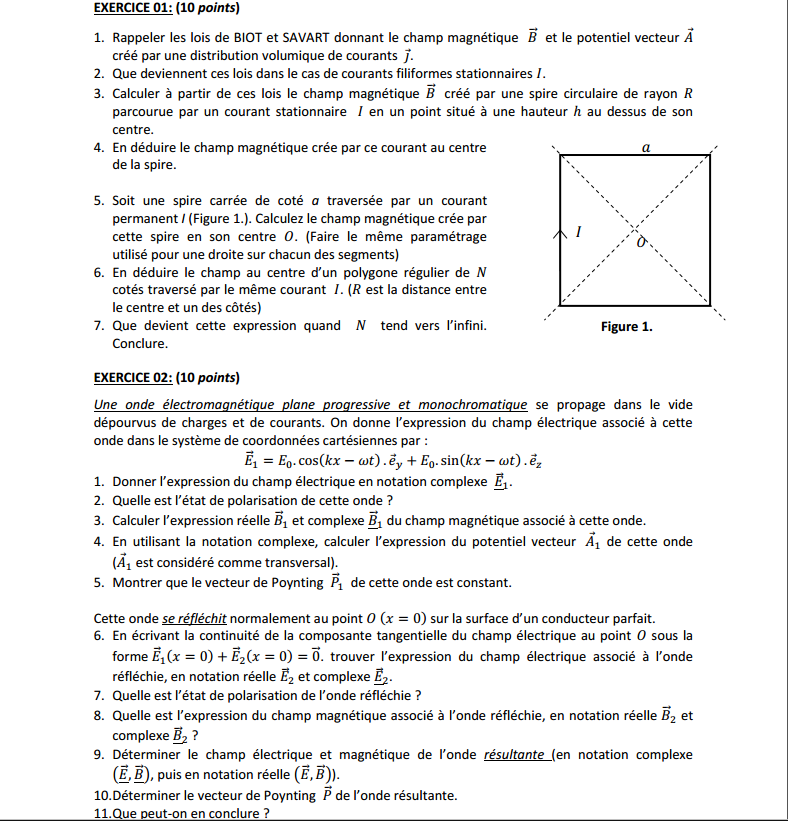
\includegraphics[width=0.9\textwidth]{images/ggg.png}
\end{center}
\end{boiteexercice}

\begin{boitecorrige}
\textbf{Questions 1 à 5 :}
\begin{center}
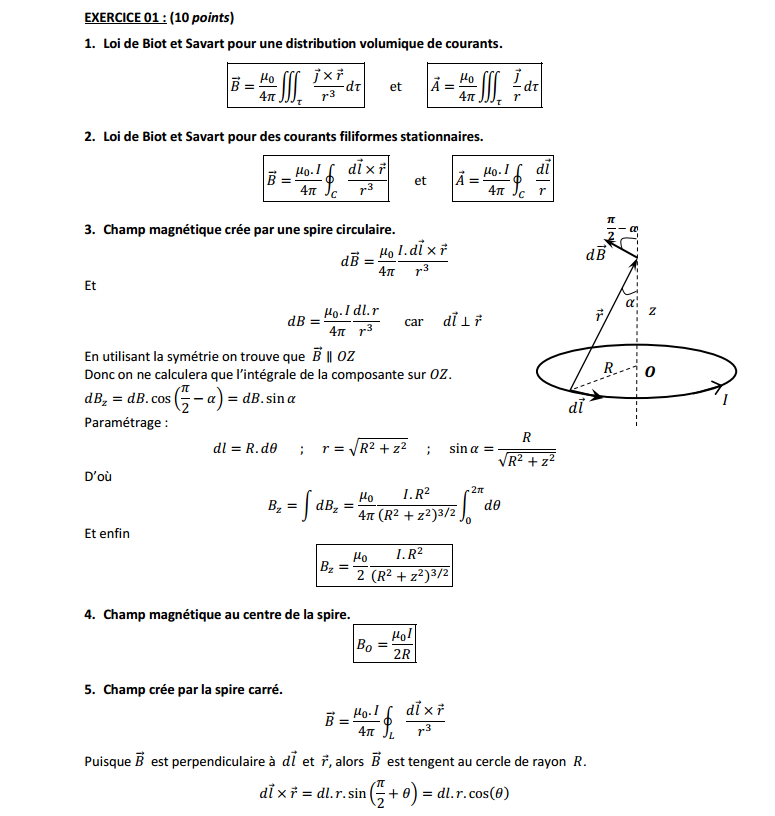
\includegraphics[width=0.92\textwidth]{images/g1.png}
\end{center}
\begin{center}
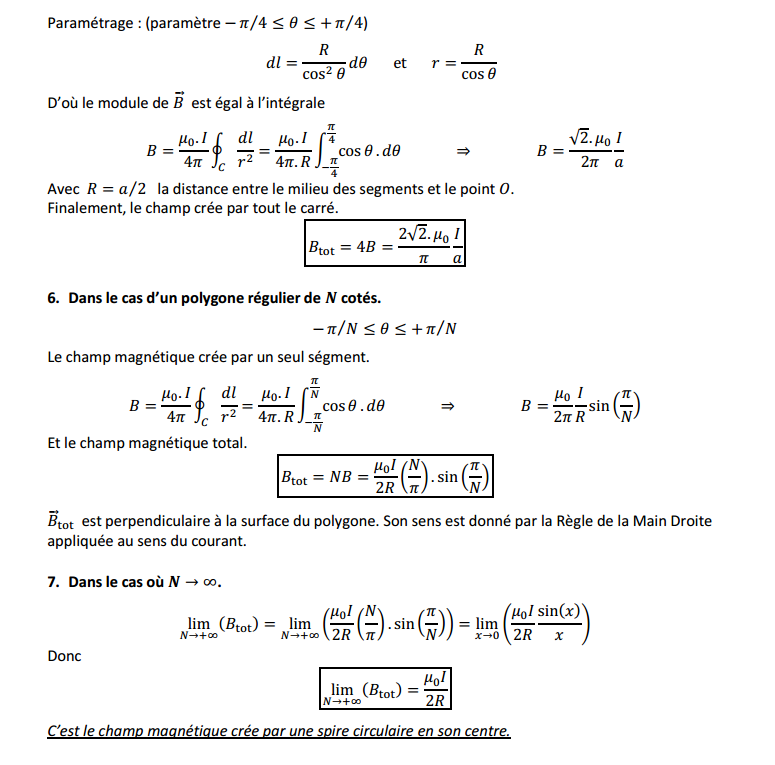
\includegraphics[width=0.92\textwidth]{images/g2.png}
\end{center}
\begin{center}
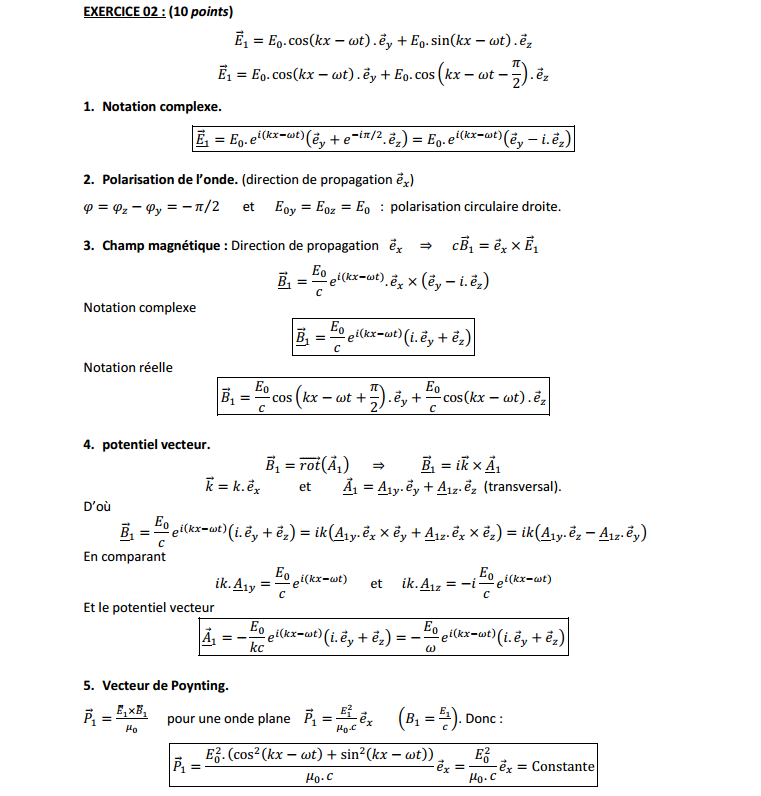
\includegraphics[width=0.92\textwidth]{images/g3.png}
\end{center}

\textbf{Question 6 :} La condition de continuité du champ électrique tangentiel à l'interface impose $\vec{E}_1(x=0) + \vec{E}_2(x=0) = \vec{0}$. L'onde $\vec{E}_2$ est une OPPH se propageant dans la direction des $x$ négatifs. On écrit sa forme générale :
\[
\vec{E}_2 = E_{0y}\cos(kx+\omega t+\varphi_y)\,\hat{e}_y + E_{0z}\cos(kx+\omega t+\varphi_z)\,\hat{e}_z
\]
La condition de continuité en $x=0$ :
\[
-E_0\cos(-\omega t)\,\hat{e}_y - E_0\cos\!\left(-\omega t-\frac{\pi}{2}\right)\hat{e}_z = E_{0y}\cos(\omega t+\varphi_y)\,\hat{e}_y + E_{0z}\cos(\omega t+\varphi_z)\,\hat{e}_z
\]

\begin{center}
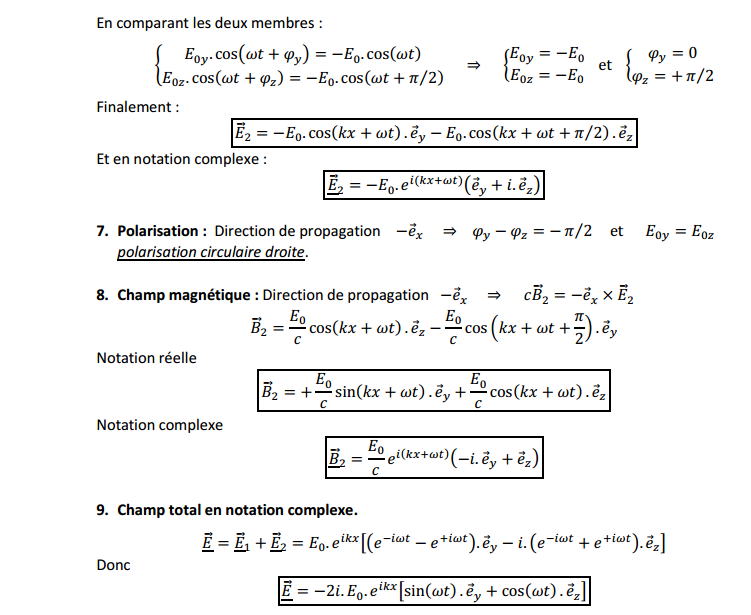
\includegraphics[width=0.9\textwidth]{images/g5.png}
\end{center}
\begin{center}
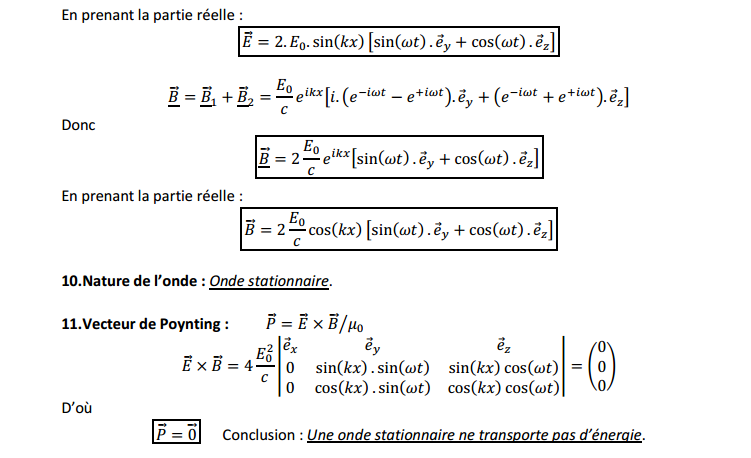
\includegraphics[width=0.9\textwidth]{images/g6.png}
\end{center}
\begin{center}
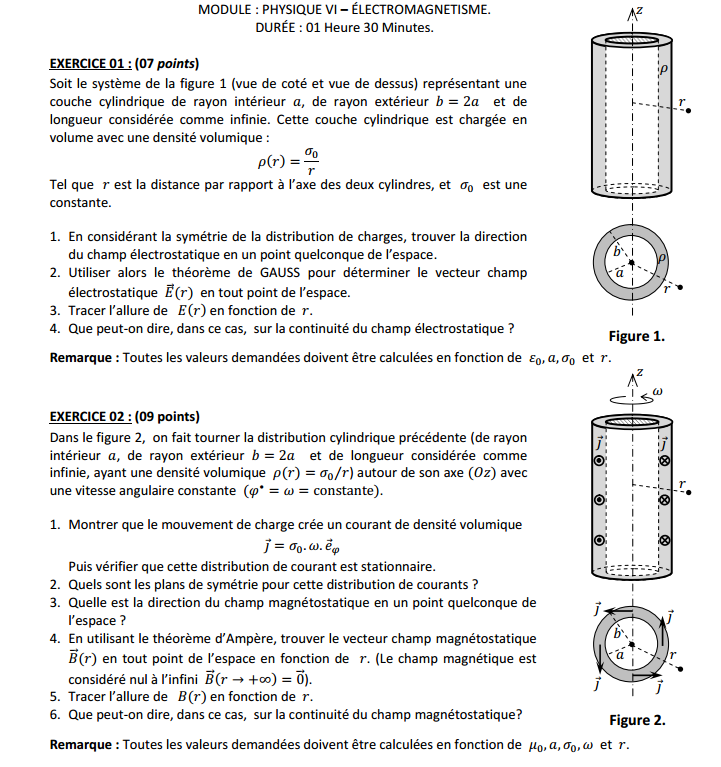
\includegraphics[width=0.9\textwidth]{images/g8.png}
\end{center}
\begin{center}
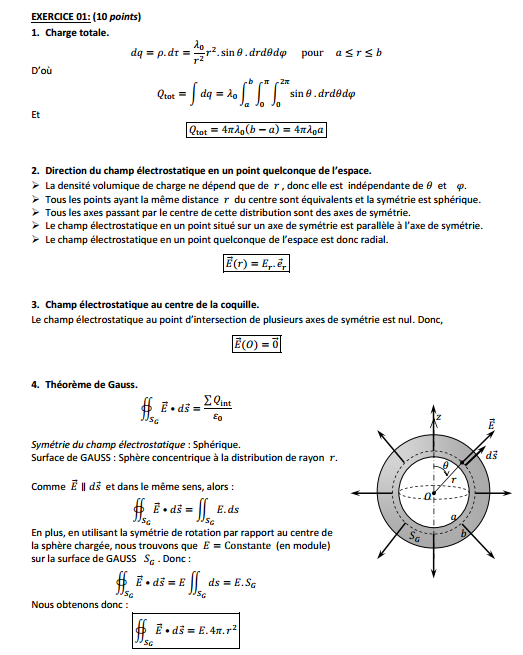
\includegraphics[width=0.9\textwidth]{images/g7.png}
\end{center}
\begin{center}
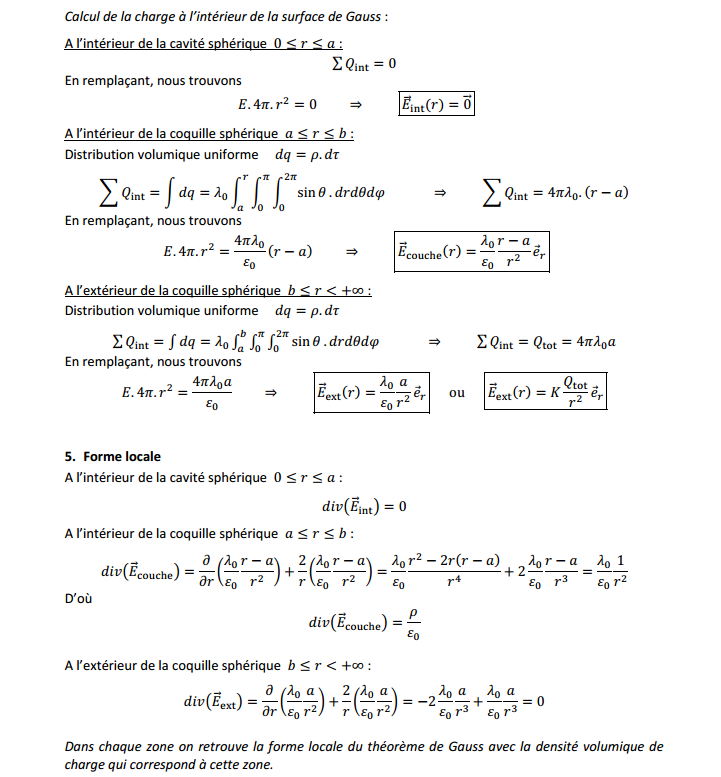
\includegraphics[width=0.9\textwidth]{images/g9.png}
\end{center}
\begin{center}
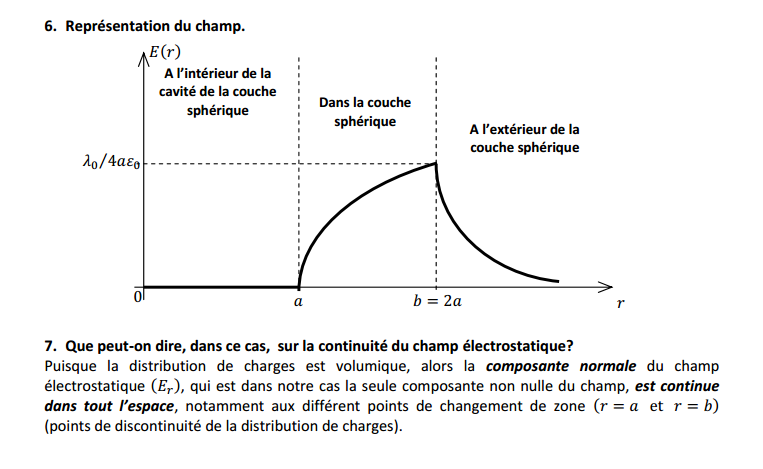
\includegraphics[width=0.9\textwidth]{images/g10.png}
\end{center}
\begin{center}
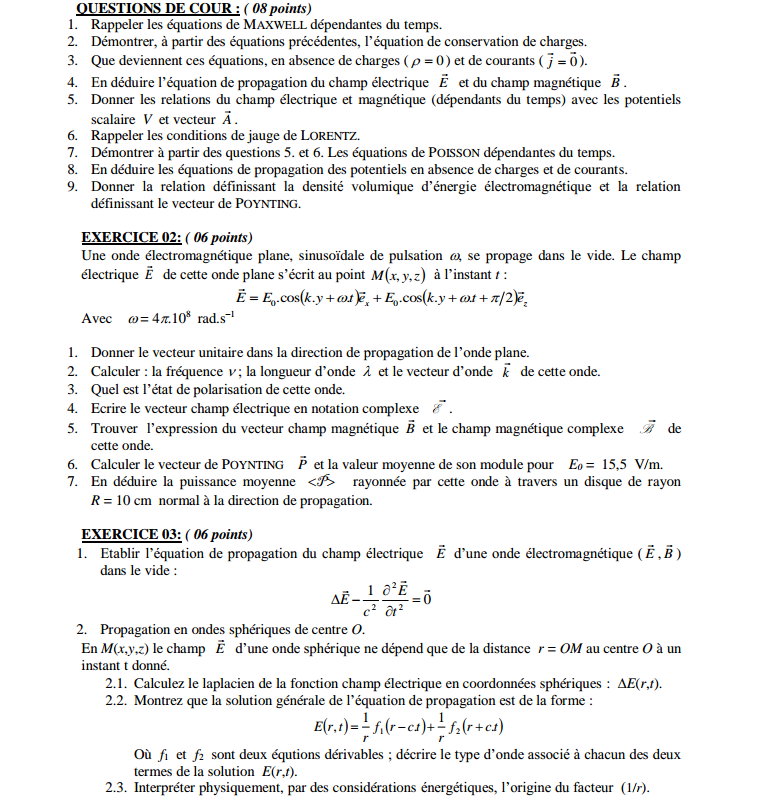
\includegraphics[width=0.9\textwidth]{images/g11.png}
\end{center}
\begin{center}
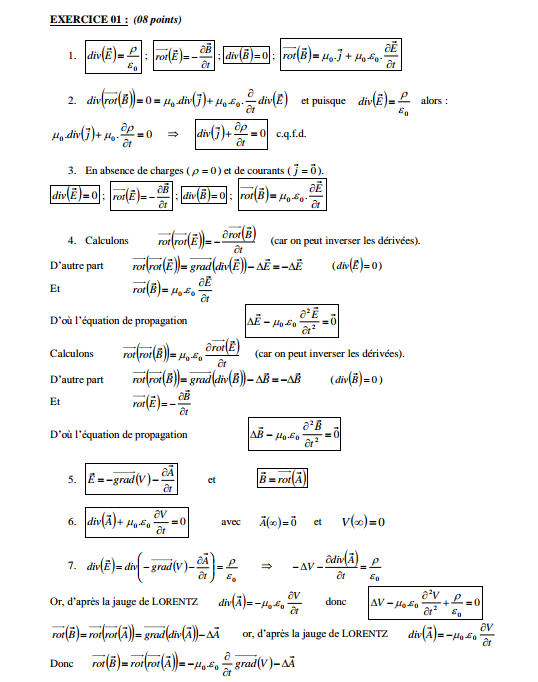
\includegraphics[width=0.9\textwidth]{images/g12.png}
\end{center}
\begin{center}
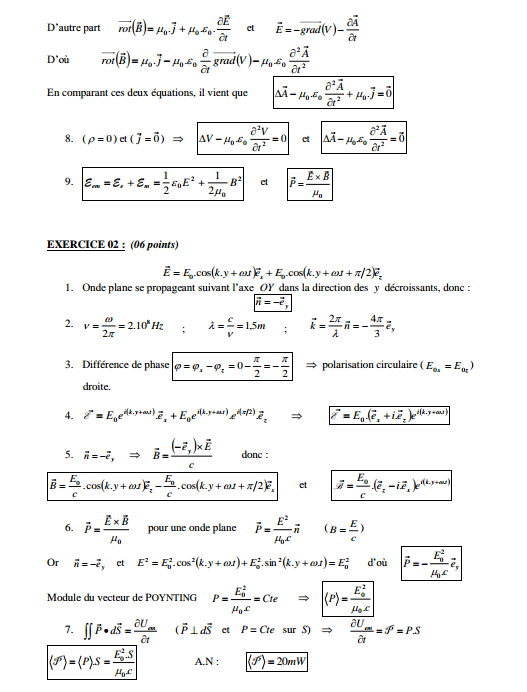
\includegraphics[width=0.9\textwidth]{images/g16.png}
\end{center}
\begin{center}
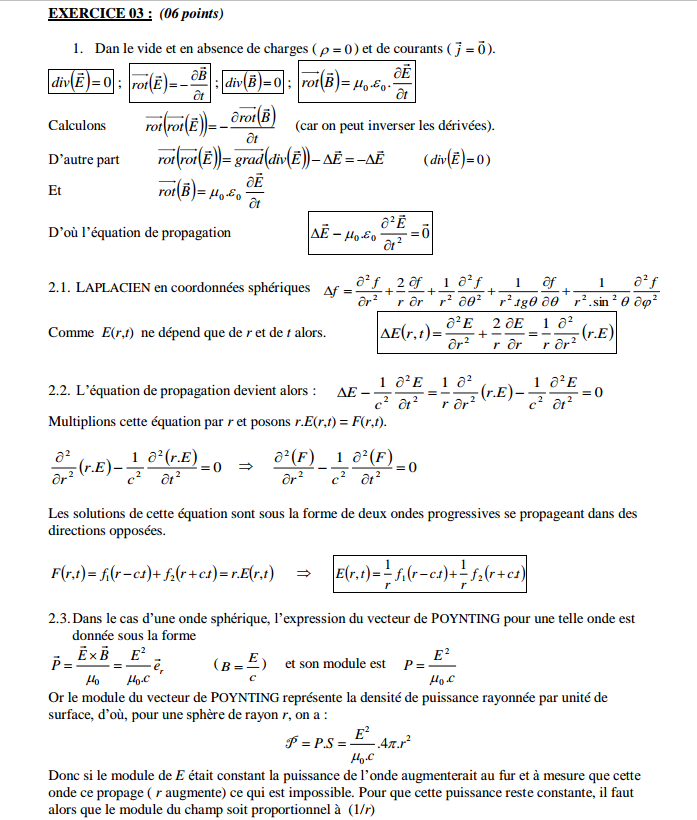
\includegraphics[width=0.9\textwidth]{images/g17.png}
\end{center}

Pour une source isotropique, la conservation de la puissance donne $\mathcal{P} = \langle\Pi\rangle\cdot 4\pi r^2 = \text{constante}$, ce qui implique $E \propto 1/r$ (le champ s'atténue en $1/r$).
\end{boitecorrige}

\section{Suppléments et exercices d'approfondissement}

\subsection*{Exercice 7 - Vecteur de Poynting et bilan d'énergie \niveau{\moyen}}

\begin{boiteexercice}
Une onde plane progressive harmonique se propage dans le vide selon $+Ox$ :
\[
\vec{E}(x,t) = E_0\cos(kx-\omega t)\,\hat{e}_y \qquad \vec{B}(x,t) = B_0\cos(kx-\omega t)\,\hat{e}_z
\]
avec $E_0 = \qty{1000}{V.m^{-1}}$.
\begin{enumerate}
  \item Exprimer $B_0$ en fonction de $E_0$ et $c$.
  \item Calculer le vecteur de Poynting instantané $\vec{\Pi} = \dfrac{1}{\mu_0}\vec{E}\wedge\vec{B}$.
  \item Calculer la moyenne temporelle $\langle\Pi\rangle$.
  \item Calculer la densité volumique d'énergie moyenne $\langle u_{em}\rangle = \langle\frac{1}{2}\varepsilon_0 E^2 + \frac{1}{2\mu_0}B^2\rangle$ et vérifier que $\langle\Pi\rangle = c\langle u_{em}\rangle$.
\end{enumerate}
\end{boiteexercice}

\begin{boitecorrige}
\textbf{1.} Pour une OPPH dans le vide, $B_0 = E_0/c$. Avec $E_0 = \qty{1000}{V.m^{-1}}$ :
\[
B_0 = \frac{1000}{3\times10^8} \approx \qty{3.33e-6}{T}
\]

\textbf{2.} Vecteur de Poynting :
\[
\vec{\Pi} = \frac{1}{\mu_0}\vec{E}\wedge\vec{B} = \frac{E_0B_0}{\mu_0}\cos^2(kx-\omega t)\,(\hat{e}_y\wedge\hat{e}_z) = \frac{E_0^2}{\mu_0 c}\cos^2(kx-\omega t)\,\hat{e}_x
\]

\textbf{3.} La moyenne temporelle de $\cos^2(\theta) = 1/2$ :
\[
\langle\Pi\rangle = \frac{E_0^2}{2\mu_0 c} = \frac{(10^3)^2}{2\times4\pi\times10^{-7}\times3\times10^8} = \frac{10^6}{240\pi} \approx \qty{1326}{W.m^{-2}}
\]

\textbf{4.} Les densités d'énergie électrique et magnétique :
\[
\langle u_E\rangle = \frac{\varepsilon_0\langle E^2\rangle}{2} = \frac{\varepsilon_0 E_0^2}{4} \qquad \langle u_B\rangle = \frac{\langle B^2\rangle}{2\mu_0} = \frac{B_0^2}{4\mu_0} = \frac{E_0^2}{4\mu_0 c^2}
\]
Comme $c^2 = 1/(\varepsilon_0\mu_0)$, on a $\langle u_B\rangle = \varepsilon_0 E_0^2/4 = \langle u_E\rangle$. Donc :
\[
\langle u_{em}\rangle = 2\langle u_E\rangle = \frac{\varepsilon_0 E_0^2}{2}
\]
Vérification : $c\langle u_{em}\rangle = c\cdot\dfrac{\varepsilon_0 E_0^2}{2} = \dfrac{E_0^2}{2\mu_0 c} = \langle\Pi\rangle$.
\end{boitecorrige}

\subsection*{Exercice 8 - Induction : flux à travers une spire en rotation \niveau{\moyen}}

\begin{boiteexercice}
Une spire rectangulaire de $N = 200$ spires et de surface $S = \qty{100}{cm^2}$ tourne à la vitesse angulaire $\omega = 2\pi\times50\,\text{rad.s}^{-1}$ dans un champ magnétique uniforme $B_0 = \qty{0.5}{T}$. L'axe de rotation est perpendiculaire au champ.
\begin{enumerate}
  \item Exprimer le flux total $\Phi(t)$ à travers la bobine.
  \item Calculer la f.é.m. induite $e(t) = -\d\Phi/\d t$.
  \item Quelle est l'amplitude de la f.é.m. ?
  \item Si la bobine alimente une résistance $R = \qty{10}{\Omega}$, calculer la puissance électrique moyenne dissipée.
\end{enumerate}
\end{boiteexercice}

\begin{boitecorrige}
\textbf{1.} Le flux à travers une spire varie sinusoïdalement :
\[
\Phi(t) = NB_0S\cos(\omega t) = 200\times0{,}5\times10^{-2}\cos(100\pi t) = \cos(100\pi t)\,\text{Wb}
\]

\textbf{2.} La f.é.m. induite :
\[
e(t) = -\deriv{\Phi}{t} = NB_0S\omega\sin(\omega t) = 1\times100\pi\sin(100\pi t)
\]
\[
e(t) = 100\pi\sin(100\pi t) \approx 314\sin(314t)\,\text{V}
\]

\textbf{3.} L'amplitude de la f.é.m. est :
\[
E_{max} = NB_0S\omega = 200\times0{,}5\times10^{-2}\times100\pi \approx \qty{314}{V}
\]

\textbf{4.} La valeur efficace de $e(t)$ est $E_{eff} = E_{max}/\sqrt{2} = 314/\sqrt{2} \approx \qty{222}{V}$.
\[
P = \frac{E_{eff}^2}{R} = \frac{(314/\sqrt{2})^2}{10} = \frac{314^2}{20} = \frac{98596}{20} \approx \qty{4930}{W}
\]
C'est le principe d'un alternateur électrique.
\end{boitecorrige}

\subsection*{Exercice 9 - Relation de dispersion dans un plasma \niveau{\difficile}}

\begin{boiteexercice}
Dans un plasma de fréquence plasma $\omega_p$, la relation de dispersion des ondes électromagnétiques est $\omega^2 = \omega_p^2 + c^2k^2$.
\begin{enumerate}
  \item Exprimer la vitesse de phase $v_\varphi = \omega/k$ et la vitesse de groupe $v_g = \d\omega/\d k$.
  \item Montrer que $v_\varphi\cdot v_g = c^2$.
  \item Pour quelle condition l'onde se propage-t-elle ? (fréquence de coupure)
  \item Calculer $v_\varphi$ et $v_g$ pour $\omega = 1{,}2\,\omega_p$ et $c = 3\times10^8\,\text{m.s}^{-1}$.
  \item Commenter : la vitesse de phase peut-elle dépasser $c$ ? L'énergie se propage-t-elle à $v_\varphi$ ou $v_g$ ?
\end{enumerate}
\end{boiteexercice}

\newpage
\begin{boitecorrige}
\textbf{1.} De $\omega^2 = \omega_p^2 + c^2k^2$, on tire $k = \sqrt{(\omega^2-\omega_p^2)/c^2}$, donc :
\[
v_\varphi = \frac{\omega}{k} = \frac{c\omega}{\sqrt{\omega^2-\omega_p^2}}
\]
Pour $v_g$, on dérive la relation de dispersion : $2\omega\,\d\omega = 2c^2k\,\d k$, soit :
\[
v_g = \frac{\d\omega}{\d k} = \frac{c^2k}{\omega} = \frac{c\sqrt{\omega^2-\omega_p^2}}{\omega}
\]

\textbf{2.} $v_\varphi\cdot v_g = \dfrac{c\omega}{\sqrt{\omega^2-\omega_p^2}}\times\dfrac{c\sqrt{\omega^2-\omega_p^2}}{\omega} = c^2$.

\textbf{3.} L'onde ne se propage que si $k$ est réel, c'est-à-dire $\omega^2 > \omega_p^2$, soit $\omega > \omega_p$. La fréquence de coupure est $\omega_p$ : en dessous, l'onde est évanescente (atténuation exponentielle).

\textbf{4.} Pour $\omega = 1{,}2\,\omega_p$ :
\[
v_\varphi = \frac{c\times1{,}2\omega_p}{\sqrt{(1{,}2)^2\omega_p^2-\omega_p^2}} = \frac{1{,}2c}{\sqrt{1{,}44-1}} = \frac{1{,}2c}{\sqrt{0{,}44}} = \frac{1{,}2c}{0{,}663} \approx 1{,}81c
\]
\[
v_g = c^2/v_\varphi = c/1{,}81 \approx 0{,}55c
\]

\textbf{5.} $v_\varphi > c$ est possible car la vitesse de phase ne transporte pas d'information ni d'énergie. L'énergie (et l'information) se propage à la vitesse de groupe $v_g < c$, conformément à la relativité. Dans un plasma, $v_g < c$ toujours.
\end{boitecorrige}

\subsection*{Exercice 10 - Lois de Snell-Descartes et coefficients de Fresnel \niveau{\difficile}}

\begin{boiteexercice}
Une onde électromagnétique se propage dans un milieu d'indice $n_1 = 1$ (air) et frappe une interface avec un milieu d'indice $n_2 = 1{,}5$ (verre). L'angle d'incidence est $\theta_i = 45°$.
\begin{enumerate}
  \item Calculer l'angle de réfraction $\theta_r$ (loi de Snell-Descartes : $n_1\sin\theta_i = n_2\sin\theta_r$).
  \item Calculer les coefficients de réflexion en amplitude pour les polarisations s (TE) et p (TM) :
  \[
  r_s = \frac{n_1\cos\theta_i - n_2\cos\theta_r}{n_1\cos\theta_i + n_2\cos\theta_r} \qquad r_p = \frac{n_2\cos\theta_i - n_1\cos\theta_r}{n_2\cos\theta_i + n_1\cos\theta_r}
  \]
  \item Calculer les réflectances $R_s = r_s^2$ et $R_p = r_p^2$.
  \item Commenter la différence entre $R_s$ et $R_p$ (angle de Brewster).
\end{enumerate}
\end{boiteexercice}

\begin{boitecorrige}
\textbf{1.} Loi de Snell-Descartes :
\[
\sin\theta_r = \frac{n_1}{n_2}\sin\theta_i = \frac{1}{1{,}5}\sin(45°) = \frac{1}{1{,}5}\times\frac{\sqrt{2}}{2} = \frac{\sqrt{2}}{3} \approx 0{,}4714
\]
\[
\theta_r = \arcsin(0{,}4714) \approx 28{,}1°
\]

\textbf{2.} Avec $\cos\theta_i = \cos(45°) = \sqrt{2}/2 \approx 0{,}7071$ et $\cos\theta_r = \cos(28{,}1°) \approx 0{,}8819$ :
\[
r_s = \frac{1\times0{,}7071 - 1{,}5\times0{,}8819}{1\times0{,}7071 + 1{,}5\times0{,}8819} = \frac{0{,}7071 - 1{,}3229}{0{,}7071 + 1{,}3229} = \frac{-0{,}6158}{2{,}030} \approx -0{,}303
\]
\[
r_p = \frac{1{,}5\times0{,}7071 - 1\times0{,}8819}{1{,}5\times0{,}7071 + 1\times0{,}8819} = \frac{1{,}0607 - 0{,}8819}{1{,}0607 + 0{,}8819} = \frac{0{,}1788}{1{,}9426} \approx 0{,}0920
\]

\textbf{3.} Réflectances :
\[
R_s = r_s^2 \approx (0{,}303)^2 \approx 0{,}092 = 9{,}2\%
\]
\[
R_p = r_p^2 \approx (0{,}0920)^2 \approx 0{,}0085 = 0{,}85\%
\]

\textbf{4.} $R_s > R_p$ : la polarisation p est beaucoup moins réfléchie. À l'angle de Brewster $\theta_B = \arctan(n_2/n_1) = \arctan(1{,}5) \approx 56{,}3°$, on a $r_p = 0$ exactement. Ce phénomène est utilisé pour produire de la lumière polarisée par réflexion.
\end{boitecorrige}

\ifdefined\inMainDoc\else\end{document}\fi


% ================================================================
%  UE 2 : THERMODYNAMIQUE
% ================================================================
\newpage
\thispagestyle{empty}
\begin{tikzpicture}[remember picture, overlay]
  \fill[gray!12] ([xshift=1.5cm, yshift=3cm]current page.south west)
    rectangle ([xshift=-1.5cm, yshift=-3cm]current page.north east);
  \draw[line width=3pt] ([xshift=1.5cm,yshift=-3cm]current page.north west)
    -- ([xshift=-1.5cm,yshift=-3cm]current page.north east);
  \draw[line width=3pt] ([xshift=1.5cm,yshift=3cm]current page.south west)
    -- ([xshift=-1.5cm,yshift=3cm]current page.south east);
  \node[align=center] at (current page.center) {%
    {\fontsize{34}{42}\bfseries\selectfont THERMODYNAMIQUE}\\[1.2cm]
    {\large\itshape Principes - Fonctions d'état}\\[0.4cm]
    {\large\itshape Machines thermiques - Cycles}\\[1.8cm]
    {\normalsize Licence 2 - UE 2}
  };
  \node[anchor=south west] at ([xshift=2cm,yshift=2cm]current page.south west)
    {\large\bfseries UE 2};
\end{tikzpicture}
\newpage

\addcontentsline{toc}{section}{THERMODYNAMIQUE}
\ifdefined\inMainDoc\else
\documentclass[12pt,a4paper]{article}
% ================================================================
%  PRÉAMBULE COMMUN - ANNALES CORRIGÉES
%  Université de Kara - FaST - Licence Fondamentale MPC
%  Design optimisé impression noir et blanc
% ================================================================

% -- ENCODAGE & LANGUE --
\usepackage[utf8]{inputenc}
\usepackage[T1]{fontenc}
\usepackage[french]{babel}
\usepackage{lmodern}
\usepackage{microtype}

% -- MISE EN PAGE --
\usepackage[a4paper, top=2.8cm, bottom=2.5cm, left=2.5cm, right=2.5cm, headheight=14pt]{geometry}
\usepackage{setspace}
\setstretch{1.2}
\usepackage{parskip}
\setlength{\parindent}{1.2em}
\setlength{\parskip}{4pt}

% -- MATHS --
\usepackage{amsmath, amssymb, mathtools, amsthm}
\usepackage{mathrsfs}
\usepackage{dsfont}
\usepackage{bm}
\usepackage{cancel}
\usepackage{textcomp}
% Définition de \oiint (intégrale de surface fermée) sans package supplémentaire
\newcommand{\oiint}{\mathop{\iint\!\!\!\!\!\!\!\bigcirc}\limits}

% -- PHYSIQUE & CHIMIE --
\usepackage{physics}
\usepackage{siunitx}
% Lorsque physics est chargé, siunitx omet \qty. On le restaure ici :
\AtBeginDocument{\RenewCommandCopy\qty\SI}
\sisetup{locale = FR, detect-all, output-decimal-marker={,}}
% Commande de substitution pour les unités posant problème avec pdflatex
% (ohm, degreeCelsius, micro, angstrom, percent utilisent des caractères non-ASCII)
\newcommand{\qtyohm}[1]{\ensuremath{\num{#1}\,\Omega}}
\newcommand{\qtydegc}[1]{\ensuremath{\num{#1}\,{}^\circ\text{C}}}
\newcommand{\qtyangstrom}[1]{\ensuremath{\num{#1}\,\text{\AA}}}
\newcommand{\qtypercent}[1]{\ensuremath{\num{#1}\,\%}}
\newcommand{\qtyum}[1]{\ensuremath{\num{#1}\,\mu\text{m}}}
\usepackage[version=4]{mhchem}

% -- GRAPHISMES --
\usepackage{graphicx}
\usepackage{float}
\usepackage{caption}
\usepackage{subcaption}
\usepackage{wrapfig}
\usepackage{tikz}
\usetikzlibrary{calc, arrows.meta, patterns, shapes.geometric}
\usepackage{pgfplots}
\pgfplotsset{compat=1.18}

% -- TABLEAUX --
\usepackage{booktabs}
\usepackage{array}
\usepackage{tabularx}
\usepackage{multirow}

% -- LISTES --
\usepackage{enumitem}
\setlist[enumerate]{topsep=3pt, itemsep=2pt, parsep=0pt}
\setlist[itemize]{topsep=3pt, itemsep=2pt, parsep=0pt, label={.}}

% -- BOÎTES (noir et blanc) --
\usepackage{mdframed}
\usepackage{tcolorbox}
\tcbuselibrary{skins, breakable, theorems}

% Boîte EXERCICE : encadré avec filet épais, fond blanc
\newmdenv[
  linewidth=1.2pt,
  linecolor=black,
  roundcorner=3pt,
  skipabove=10pt,
  skipbelow=6pt,
  innertopmargin=8pt,
  innerbottommargin=8pt,
  innerleftmargin=10pt,
  innerrightmargin=10pt,
  backgroundcolor=white,
  frametitle={\bfseries\small Exercice},
  frametitlealignment=\raggedright,
  frametitleaboveskip=4pt,
  frametitlebelowskip=4pt,
]{boiteexercice}

% Boîte CORRIGÉ : fond gris très clair + filet fin
\newmdenv[
  linewidth=0.6pt,
  linecolor=black,
  leftline=true,
  rightline=false,
  topline=false,
  bottomline=false,
  linecolor=black,
  innerleftmargin=12pt,
  innerrightmargin=8pt,
  innertopmargin=6pt,
  innerbottommargin=6pt,
  backgroundcolor=gray!8,
  skipabove=4pt,
  skipbelow=8pt,
]{boitecorrige}

% Boîte RÉSUMÉ DE COURS : double encadré
\newmdenv[
  linewidth=0.8pt,
  linecolor=black,
  roundcorner=2pt,
  backgroundcolor=gray!12,
  innertopmargin=10pt,
  innerbottommargin=10pt,
  innerleftmargin=12pt,
  innerrightmargin=12pt,
  skipabove=12pt,
  skipbelow=8pt,
]{boiteresume}

% Boîte ATTENTION/REMARQUE : barre gauche épaisse
\newmdenv[
  leftline=true,
  rightline=false,
  topline=false,
  bottomline=false,
  linewidth=3pt,
  linecolor=black,
  backgroundcolor=gray!5,
  innerleftmargin=12pt,
  innerrightmargin=8pt,
  innertopmargin=5pt,
  innerbottommargin=5pt,
  skipabove=6pt,
  skipbelow=6pt,
]{boiteremarque}

% -- DIFFICULTÉ DES EXERCICES --
\newcommand{\facile}{$\star$}
\newcommand{\moyen}{$\star\!\star$}
\newcommand{\difficile}{$\star\!\star\!\star$}
\newcommand{\niveau}[1]{\hfill\textbf{#1}\hspace{2pt}}

% -- EN-TÊTES ET PIEDS DE PAGE --
\usepackage{fancyhdr}
\pagestyle{fancy}
\fancyhf{}
\renewcommand{\headrulewidth}{0.5pt}
\renewcommand{\footrulewidth}{0.3pt}

% -- HYPERLIENS --
\usepackage[hidelinks]{hyperref}
\hypersetup{
    colorlinks=false,
    pdftitle={Annale Corrigée - Licence MPC - Université de Kara}
}

% -- TITRES --
\usepackage{titlesec}
\titleformat{\section}{\Large\bfseries}{\thesection.}{0.8em}{}[\vspace{2pt}\hrule\vspace{4pt}]
\titleformat{\subsection}{\large\bfseries}{\thesubsection.}{0.7em}{}
\titleformat{\subsubsection}{\normalsize\bfseries}{\thesubsubsection.}{0.6em}{}

% -- THÉORÈMES --
\theoremstyle{definition}
\newtheorem{defn}{Définition}[section]
\newtheorem{prop}{Propriété}[section]
\newtheorem{thm}{Théorème}[section]
\newtheorem{corol}{Corollaire}[section]
\newtheorem{exemple}{Exemple}[section]

% -- COMMANDES MATHÉMATIQUES UTILES --
\newcommand{\vect}[1]{\overrightarrow{#1}}
\newcommand{\R}{\mathbb{R}}
\newcommand{\N}{\mathbb{N}}
\newcommand{\Z}{\mathbb{Z}}
\newcommand{\C}{\mathbb{C}}
\renewcommand{\d}{\mathrm{d}}
\newcommand{\deriv}[2]{\dfrac{\d #1}{\d #2}}
\newcommand{\dpart}[2]{\dfrac{\partial #1}{\partial #2}}
\newcommand{\rot}{\overrightarrow{\mathrm{rot}}\,}
\renewcommand{\div}{\mathrm{div}\,}
\renewcommand{\grad}{\overrightarrow{\mathrm{grad}}\,}
\newcommand{\e}{\mathrm{e}}
\newcommand{\ii}{\mathrm{i}}
\renewcommand{\Tr}{\mathrm{Tr}}

% Numérotation des équations par section
\numberwithin{equation}{section}

% -- RÉSULTATS ENCADRÉS --
\newcommand{\res}[1]{\[\boxed{#1}\]}

% -- REMARQUE INLINE --
\newcommand{\rmq}[1]{\begin{boiteremarque}\textbf{Remarque.} #1\end{boiteremarque}}

% -- MISE EN VALEUR DU RÉSULTAT FINAL --
\newcommand{\reponse}[1]{%
  \begin{center}
    \fbox{\begin{minipage}{0.92\textwidth}\centering #1\end{minipage}}
  \end{center}%
}


\lhead{\small\textit{Thermodynamique - Licence 2}}
\rhead{\small\textit{FaST, Université de Kara}}
\cfoot{\thepage}

\begin{document}
\fi

\begin{center}
  {\LARGE\bfseries THERMODYNAMIQUE CLASSIQUE}\\[0.3cm]
  {\normalsize Licence 2 - Mathématiques, Physique et Chimie}\\[0.1cm]
  \rule{0.7\textwidth}{0.8pt}
\end{center}

\vspace{0.3cm}

\section*{Résumé du cours}

\begin{boiteresume}

\textbf{1. Premier principe de la thermodynamique.}
\[
\d U = \delta W + \delta Q \qquad \text{ou sous forme finie :} \qquad \Delta U = W + Q
\]
Pour une transformation réversible : $\delta W = -P\,\d V$ et $\delta Q = T\,\d S$.

\textbf{2. Fonctions d'état dérivées.}
\begin{itemize}[nosep]
  \item Enthalpie : $H = U + PV$ ; $\d H = T\,\d S + V\,\d P$.
  \item Énergie libre (Helmholtz) : $F = U - TS$ ; $\d F = -S\,\d T - P\,\d V$.
  \item Enthalpie libre (Gibbs) : $G = H - TS$ ; $\d G = -S\,\d T + V\,\d P$.
\end{itemize}

\textbf{3. Relations de Maxwell.} Elles découlent de l'égalité des dérivées croisées :
\[
\left(\dpart{S}{V}\right)_T = \left(\dpart{P}{T}\right)_V \qquad \left(\dpart{S}{P}\right)_T = -\left(\dpart{V}{T}\right)_P
\]

\textbf{4. Coefficients thermoélastiques.}
\[
\alpha = \frac{1}{V}\left(\dpart{V}{T}\right)_P \quad (\text{dilat. isobare}) \qquad \chi_T = -\frac{1}{V}\left(\dpart{V}{P}\right)_T \quad (\text{compress. isoth.})
\]

\textbf{5. Gaz de van der Waals.}
\[
\left(P + \frac{a}{V^2}\right)(V - b) = nRT
\]
où $a$ tient compte des interactions attractives et $b$ du volume propre des molécules.

\textbf{6. Transformations des gaz parfaits.} Pour un gaz parfait diatomique ($\gamma = 7/5$), lors d'une détente adiabatique réversible : $TV^{\gamma-1} = \text{cste}$ et $TP^{(1-\gamma)/\gamma} = \text{cste}$.

\end{boiteresume}

\newpage

\section{Fonctions d'état et relations thermodynamiques}

\subsection*{Exercice 1 \niveau{\moyen}}

\begin{boiteexercice}
On considère la fonction $F(x,y,z)$ dont la différentielle est :
\[
\d F = (2x-y)\,\d x - (x-2y)\,\d y - 4z\,\d z
\]
\begin{enumerate}
  \item Retrouver $F(x,y,z)$ à une constante $a$ près.
  \item Déterminer les valeurs de $a$ si $F(a,2,-1) = 2$.
  \item Écrire les formes possibles de $F$.
\end{enumerate}
\end{boiteexercice}

\begin{boitecorrige}
\textbf{1.} On identifie les dérivées partielles :
\[
\dpart{F}{x} = 2x-y, \qquad \dpart{F}{y} = 2y-x, \qquad \dpart{F}{z} = -4z
\]
En intégrant la première relation par rapport à $x$ :
\[
F = x^2 - xy + C(y,z)
\]
En substituant dans la deuxième : $\partial C/\partial y = 2y$, donc $C(y,z) = y^2 + k(z)$.

En substituant dans la troisième : $k'(z) = -4z$, donc $k(z) = -2z^2 + a$.

\[
\boxed{F(x,y,z) = x^2 + y^2 - 2z^2 - xy + a}
\]

\textbf{2.} En appliquant la condition $F(a,2,-1) = 2$ :
\[
a^2 + 4 - 2 - 2a + a = 2 \quad \Rightarrow \quad a^2 - a = 0 \quad \Rightarrow \quad a(a-1) = 0
\]
Donc $a = 0$ ou $a = 1$.

\textbf{3.}
\begin{itemize}
  \item Pour $a=0$ : $F(x,y,z) = x^2 + y^2 - 2z^2 - xy$.
  \item Pour $a=1$ : $F(x,y,z) = x^2 + y^2 - 2z^2 - xy + 1$.
\end{itemize}
\end{boitecorrige}

\subsection*{Exercice 2 - Compressions successives d'un gaz parfait diatomique \niveau{\difficile}}

\begin{boiteexercice}
On comprime isotherme un gaz parfait diatomique de $P_0$ à $P_1$ à la température $T_0$, puis on le détend adiabatiquement et réversiblement jusqu'à $P_0$.

\begin{enumerate}
  \item Exprimer la température $T_1$ atteinte après cette double opération.
  \item (a) Après une deuxième double opération depuis $T_1$, exprimer $T_2$. \newline
        (b) Donner une expression générale de $T_n$. \newline
        (c) Calculer $T_1$, $T_2$ et $T_{100}$ pour $P_1/P_0 = 2$ et $T_0 = \qty{300}{K}$, $\gamma = 7/5$. \newline
        (d) $T_\infty$ est-elle en accord avec le troisième principe ?
  \item Pour la $n$-ième double opération, exprimer la chaleur $Q_n$, le travail $W_n$ et $\Delta U_n$.
  \item Après $n$ doubles opérations, calculer $Q$, $W$ et $\Delta U$ totaux.
\end{enumerate}
\end{boiteexercice}

\begin{boitecorrige}
\textbf{1.} L'isotherme amène de $(P_0, T_0)$ à $(P_1, T_0)$ : la température ne change pas. La détente adiabatique réversible de $(P_1, T_0)$ à $(P_0, T_1)$ suit $T P^{(1-\gamma)/\gamma} = \text{cste}$ :
\[
T_1 P_0^{(1-\gamma)/\gamma} = T_0 P_1^{(1-\gamma)/\gamma} \quad \Rightarrow \quad \boxed{T_1 = T_0\left(\frac{P_1}{P_0}\right)^{(1-\gamma)/\gamma}}
\]
Comme $P_1 > P_0$ et $(1-\gamma)/\gamma < 0$, on a $T_1 < T_0$ : le gaz se refroidit.

\textbf{2.(a)} En répétant la même logique depuis $T_1$ :
\[
T_2 = T_1\left(\frac{P_1}{P_0}\right)^{(1-\gamma)/\gamma} = T_0\left(\frac{P_1}{P_0}\right)^{2(1-\gamma)/\gamma}
\]

\textbf{2.(b)} Par récurrence :
\[
\boxed{T_n = T_0\left(\frac{P_1}{P_0}\right)^{n(1-\gamma)/\gamma}}
\]

\textbf{2.(c)} Avec $P_1/P_0 = 2$, $\gamma = 7/5$ : $(1-\gamma)/\gamma = (1-7/5)/(7/5) = (-2/5)/(7/5) = -2/7$.
\[
T_1 = 300\times 2^{-2/7} \approx 300\times 0{,}820 \approx \qty{246}{K}
\]
\[
T_2 \approx 246\times 0{,}820 \approx \qty{202}{K} \qquad T_{100} = 300\times 2^{-200/7} \approx \qty{0}{K}
\]

\textbf{2.(d)} $T_\infty = 0$, ce qui serait atteindre le zéro absolu par un processus cyclique. Ceci est en accord avec la direction imposée par le troisième principe (on tend vers $0\,K$), mais le troisième principe affirme qu'on ne peut pas atteindre $0\,K$ en un nombre fini d'opérations ; ici, $n\to\infty$ est requis, ce qui est physiquement inaccessible. Il n'y a donc pas de contradiction.

\textbf{3.} Pour la $n$-ième double opération (isotherme puis adiabatique) :

\emph{\'Etape isotherme} $(T_{n-1},\, P_0 \to P_1)$ :
$\Delta U = 0$ pour un gaz parfait.
Le travail et la chaleur sont
\[
W_{\text{isoth}} = nRT_{n-1}\ln(P_0/P_1),
\qquad
Q_n = -W_{\text{isoth}} = nRT_{n-1}\ln(P_1/P_0).
\]

\emph{\'Etape adiabatique} $(P_1,\, T_{n-1} \to P_0,\, T_n)$ :
$Q = 0$ et $W_{\text{adia}} = nC_v(T_n - T_{n-1})$.

Bilan de la $n$-ième double opération :
\[
Q_n = nRT_{n-1}\ln\!\left(\frac{P_1}{P_0}\right), \quad W_n = nC_v(T_n-T_{n-1}) - nRT_{n-1}\ln\!\left(\frac{P_1}{P_0}\right)
\]
\[
\Delta U_n = nC_v(T_n - T_{n-1})
\]

\textbf{4.} En sommant sur $n$ opérations :
\[
\Delta U = nC_v(T_n - T_0) \qquad Q = nR\ln\!\left(\frac{P_1}{P_0}\right)\sum_{k=0}^{n-1}T_k \qquad W = \Delta U - Q
\]
\end{boitecorrige}

\subsection*{Exercice 3 - Coefficients thermoélastiques et équation d'état \niveau{\difficile}}

\begin{boiteexercice}
Des mesures sur une mole d'azote ont donné :
\[
\alpha = \frac{R}{RT+bP} \qquad (1) \qquad \chi_T = \frac{RT}{(RT+bP)P} \qquad (2)
\]
où $b$ est une constante positive homogène à un volume.

\begin{enumerate}
  \item Rappeler les expressions de $\alpha$ et $\chi_T$.
  \item Montrer que (1) après intégration donne $V = (RT+bP)\varphi(P)$ où $\varphi$ est une fonction de $P$ seul.
  \item Vérifier la cohérence avec (2).
  \item Déduire que $\varphi(P) = a/P$ et donner la valeur de $a$ pour que le gaz soit parfait à basse pression.
  \item Écrire l'équation d'état d'une mole.
\end{enumerate}
\end{boiteexercice}

\begin{boitecorrige}
\textbf{1.}
\[
\alpha = \frac{1}{V}\left(\dpart{V}{T}\right)_P \qquad \chi_T = -\frac{1}{V}\left(\dpart{V}{P}\right)_T
\]

\textbf{2.} De $\alpha = R/(RT+bP)$, on tire $\left(\dpart{V}{T}\right)_P = \alpha V = \frac{RV}{RT+bP}$, donc $\frac{\d V}{V} = \frac{R\,\d T}{RT+bP}$ à $P$ constant. En intégrant par rapport à $T$ : $\ln V = \ln(RT+bP) + f(P)$, soit $V = (RT+bP)\e^{f(P)} = (RT+bP)\varphi(P)$ avec $\varphi(P) = \e^{f(P)}$.

\textbf{3.} $\left(\dpart{V}{P}\right)_T = (b\cdot\varphi + (RT+bP)\varphi')$. Le coefficient $\chi_T$ vaut :
\[
\chi_T = -\frac{1}{V}\left(\dpart{V}{P}\right)_T = -\frac{b\varphi + (RT+bP)\varphi'}{(RT+bP)\varphi}
\]
En égalant avec (2) : $b/(RT+bP) + \varphi'/\varphi = -RT/[(RT+bP)P]$, d'où $\varphi'/\varphi = -1/P$, soit $\varphi(P) = a/P$ (après intégration).

\textbf{4.} Pour $b\to0$ : $V = aRT/P$. La loi des gaz parfaits donne $PV = RT$, donc $a = 1$.

\textbf{5.} L'équation d'état d'une mole est :
\[
\boxed{V = \frac{RT+bP}{P} = \frac{RT}{P} + b}
\]
Ce qui s'écrit aussi $P(V-b) = RT$ : c'est un modèle simplifié qui tient compte du volume propre mais pas des interactions attractives.
\end{boitecorrige}

\subsection*{Exercice 4 - Fluide homogène monophasé \niveau{\difficile}}

\begin{boiteexercice}
On considère $n$ moles d'un fluide homogène monophasé.

\textbf{Partie A.}
\begin{enumerate}
  \item Écrire $\d U$ en fonction de $\d T, \d V$, puis en fonction de $\d V, \d S$.
  \item En déduire $(\partial S/\partial T)_V$ et $(\partial S/\partial V)_T$.
  \item Montrer que $(\partial S/\partial V)_T = (\partial P/\partial T)_V$ et que la chaleur latente $\ell = T(\partial P/\partial T)_V$.
\end{enumerate}

\textbf{Partie B.} Le fluide est un gaz de van der Waals : $P = \dfrac{nRT}{V-nb} - \dfrac{n^2 a}{V^2}$.
\begin{enumerate}
  \item Calculer le travail $W_{R,T}$ et la variation d'énergie interne $\Delta U_{R,T}$ lors d'une transformation réversible isotherme de $V_i$ à $V_f$.
  \item En déduire la chaleur échangée $Q_{R,T}$.
\end{enumerate}
\end{boiteexercice}

\begin{boitecorrige}
\textbf{A.1.} En utilisant $U = U(T,V)$ :
\[
\d U = \left(\dpart{U}{T}\right)_V\d T + \left(\dpart{U}{V}\right)_T\d V = nC_v\d T + \ell_v\d V
\]
où $\ell_v = (\partial U/\partial V)_T$ est la chaleur latente volumique. En thermodynamique des processus réversibles : $\d U = T\d S - P\d V$.

\textbf{A.2.} Par identification des deux expressions de $\d U$ :
\[
\left(\dpart{S}{T}\right)_V = \frac{nC_v}{T} \qquad \left(\dpart{S}{V}\right)_T = \frac{\ell_v + P}{T}
\]

\textbf{A.3.} L'énergie libre $F = U - TS$ donne $\d F = -S\d T - P\d V$. L'égalité des dérivées croisées conduit à $(\partial S/\partial V)_T = (\partial P/\partial T)_V$ (relation de Maxwell). Or $\ell_v + P = T(\partial P/\partial T)_V$, d'où $\ell = \ell_v = T(\partial P/\partial T)_V - P$.

\textbf{B.1.} Pour van der Waals : $(\partial P/\partial T)_V = nR/(V-nb)$, donc $\ell_v = T\cdot nR/(V-nb) - P = n^2a/V^2$ (substitution de $P$). Ainsi $\d U = nC_v\d T + (n^2a/V^2)\d V$.

Lors d'une transformation isotherme ($\d T = 0$) :
\[
\Delta U_{R,T} = \int_{V_i}^{V_f}\frac{n^2 a}{V^2}\d V = n^2 a\left(\frac{1}{V_i}-\frac{1}{V_f}\right)
\]

Le travail échangé :
\begin{align*}
W_{R,T} &= -\int_{V_i}^{V_f}P\,\d V\\
        &= -\int_{V_i}^{V_f}\!\left(\frac{nRT}{V-nb}-\frac{n^2 a}{V^2}\right)\d V\\
        &= -nRT\ln\frac{V_f-nb}{V_i-nb} - n^2 a\!\left(\frac{1}{V_i}-\frac{1}{V_f}\right)
\end{align*}

\textbf{B.2.} Par le premier principe : $Q_{R,T} = \Delta U_{R,T} - W_{R,T} = nRT\ln\dfrac{V_f-nb}{V_i-nb}$.
\end{boitecorrige}

\subsection*{Exercice 5 - Gaz de van der Waals : transformations \niveau{\difficile}}

\begin{boiteexercice}
On considère une mole de gaz : $(P+a/V^2)(V-b) = RT$.
\begin{enumerate}
  \item Donner les expressions différentielles de $\d U$ et $\d S$ en fonction de $C_V$, $\ell$, $P$, $T$, $\d T$ et $\d V$.
  \item Exprimer $\ell$ en fonction de $P$, $a$ et $V$.
  \item Calculer $\Delta U$ entre $(P_1,V_1,T_1)$ et $(P_2,V_2,T_2)$ avec $C_V$ constant.
  \item Calculer $\Delta S$ pour la même transformation.
  \item Établir l'équation de l'adiabatique réversible. La simplifier si $a/V^2 \ll P$ et $b \ll V$.
\end{enumerate}
\end{boiteexercice}

\begin{boitecorrige}
\textbf{1.} Les expressions générales des différentielles en variables $(T,V)$ sont :
\[
\d U = C_V\,\d T + \ell\,\d V \qquad \d S = \frac{C_V}{T}\,\d T + \frac{\ell+P}{T}\,\d V
\]

\textbf{2.} Pour van der Waals : $\ell = T\left(\dpart{P}{T}\right)_V - P = \frac{T\cdot R}{V-b} - P = \frac{TR}{V-b} - \frac{RT}{V-b} + \frac{a}{V^2} = \frac{a}{V^2}$.

\textbf{3.}
\[
\Delta U = C_V(T_2-T_1) + a\!\left(\frac{1}{V_1}-\frac{1}{V_2}\right)
\]

\textbf{4.}
\[
\Delta S = C_V\ln\frac{T_2}{T_1} + R\ln\frac{V_2-b}{V_1-b}
\]

\textbf{5.} Pour une adiabatique réversible $\d S = 0$ :
\[
C_V\,\d T + \frac{a}{V^2}\,\d V = 0 \quad \text{(énergie interne)} \quad \text{et} \quad C_V\frac{\d T}{T} + R\frac{\d V}{V-b} = 0
\]
En intégrant la deuxième relation : $T(V-b)^R/C_V = \text{cste}$, soit $T(V-b)^{\gamma-1} = \text{cste}$.

Pour $a/V^2 \ll P$ et $b \ll V$ : $T V^{\gamma-1} = \text{cste}$ (loi de Poisson classique pour un gaz parfait).
\end{boitecorrige}

\section{Entropie et second principe}

\subsection*{Exercice 6 - Échange thermique irréversible \niveau{\facile}}

\begin{boiteexercice}
Un morceau d'aluminium froid $A$ de masse $m = \qty{100}{g}$ à la température $T_1 = \qty{10}{\celsius}$ est mis en contact thermique avec l'air ambiant $B$ (thermostat) à $T_2 = \qty{20}{\celsius}$.
\begin{enumerate}
  \item Calculer la variation d'entropie $\Delta S_A$ du morceau d'aluminium.
  \item Calculer la variation d'entropie $\Delta S_B$ de l'air ambiant.
  \item Déduire $\Delta S_{A+B}$ de l'univers. La transformation est-elle réversible ?
\end{enumerate}
Donnée : $C_{\rm Al} = \qty{896}{J.kg^{-1}.K^{-1}}$.
\end{boiteexercice}

\begin{boitecorrige}
\textbf{1.} La température finale de l'aluminium est $T_f = T_2 = \qty{293}{K}$, et $T_1 = \qty{283}{K}$.
\[
\Delta S_A = \int_{T_1}^{T_f}\frac{mC\,\mathrm{d}T}{T} = mC\ln\frac{T_f}{T_1} = 0{,}100\times896\times\ln\frac{293}{283}
\]
\[
\boxed{\Delta S_A \approx \qty{3.11e-1}{J.K^{-1}}}
\]

\textbf{2.} $B$ est un thermostat ; la chaleur cédée par $B$ est $Q_B = -Q_A = -mC(T_f-T_1)$.
\[
\Delta S_B = \frac{Q_B}{T_2} = -\frac{mC(T_f-T_1)}{T_2} = -\frac{0{,}100\times896\times10}{293}
\]
\[
\boxed{\Delta S_B \approx -\qty{3.06e-1}{J.K^{-1}}}
\]

\textbf{3.}
\[
\Delta S_{A+B} = \Delta S_A + \Delta S_B \approx 3{,}11\times10^{-1} - 3{,}06\times10^{-1} = \qty{5.4e-3}{J.K^{-1}} > 0
\]
$\Delta S_{A+B} > 0$ pour ce système isolé : la transformation est \textbf{irréversible}, conformément au second principe.
\end{boitecorrige}

\subsection*{Exercice 7 - Cycle d'Ericsson \niveau{\difficile}}

\begin{boiteexercice}
Un moteur thermique contenant $n$ moles de gaz parfait ($\gamma$ constant) décrit le cycle d'Ericsson :
\begin{itemize}[nosep]
  \item $AB$ : isotherme à $T_2$ de $P_A=P_1$ à $P_B=P_2$ ($P_2>P_1$)
  \item $BC$ : isobare $P_2$ de $T_2$ à $T_1$ ($T_1>T_2$)
  \item $CD$ : isotherme à $T_1$ jusqu'à $P_D=P_1$
  \item $DA$ : isobare $P_1$ de $T_1$ à $T_2$
\end{itemize}
\begin{enumerate}
  \item Représenter le cycle dans les diagrammes $(P,V)$ et $(T,S)$.
  \item Montrer que $W = -nRT_1\!\left(1-\dfrac{T_2}{T_1}\right)\ln\dfrac{P_2}{P_1}$.
  \item Calculer le rendement du moteur.
  \item Avec un régénérateur (récupération totale de la chaleur isobare), calculer $Q_1$ et $Q_2$ et le rendement. Comparer au rendement de Carnot.
\end{enumerate}
\end{boiteexercice}

\begin{boitecorrige}
\textbf{1.} Dans le diagramme $(P,V)$ : deux isothermes hyperboliques (AB et CD) reliées par deux isobares. Dans le diagramme $(T,S)$ : les isobares sont des exponentielles ($T = \text{cste}\cdot e^{S/(nC_P)}$) et les isothermes sont des segments horizontaux.

\textbf{2.} Calcul des travaux élémentaires :
\begin{align*}
W_{A\to B} &= -nRT_2\ln\frac{V_B}{V_A} = -nRT_2\ln\frac{P_1}{P_2} = nRT_2\ln\frac{P_2}{P_1}\\
W_{B\to C} &= -P_2(V_C-V_B) = -nR(T_1-T_2)\\
W_{C\to D} &= -nRT_1\ln\frac{P_1}{P_2} = nRT_1\ln\frac{P_1}{P_2}\\
W_{D\to A} &= -P_1(V_A-V_D) = -nR(T_2-T_1) = nR(T_1-T_2)
\end{align*}
Les contributions isobares s'annulent ($W_{BC}+W_{DA}=0$), et :
\[
\boxed{W = nRT_2\ln\frac{P_2}{P_1} + nRT_1\ln\frac{P_1}{P_2} = -nR(T_1-T_2)\ln\frac{P_2}{P_1} = -nRT_1\!\left(1-\frac{T_2}{T_1}\right)\ln\frac{P_2}{P_1}}
\]

\textbf{3.} Les chaleurs reçues : $Q_{CD} = nRT_1\ln(P_2/P_1)$ (source chaude) et $Q_{BC} = nC_P(T_1-T_2)$ (chauffage isobare). Le rendement est :
\[
\eta = \frac{|W|}{Q_{CD}+Q_{BC}} = \frac{(T_1-T_2)\ln(P_2/P_1)}{T_1\ln(P_2/P_1)+\frac{\gamma}{\gamma-1}(T_1-T_2)} < 1-\frac{T_2}{T_1}
\]

\textbf{4.} Avec régénérateur, $Q_{BC}$ est récupéré lors de $DA$ : seules les isothermes échangent avec les sources.
\[
Q_1 = Q_{CD} = nRT_1\ln\frac{P_2}{P_1}, \qquad Q_2 = Q_{AB} = nRT_2\ln\frac{P_1}{P_2}
\]
\[
\eta = \frac{|W|}{Q_1} = 1 + \frac{Q_2}{Q_1} = 1 - \frac{T_2}{T_1} = \eta_{\rm Carnot}
\]
Le cycle d'Ericsson avec régénérateur est aussi efficace qu'un cycle de Carnot.
\end{boitecorrige}

\subsection*{Exercice 8 - Machine à vapeur et rendement de Carnot \niveau{\facile}}

\begin{boiteexercice}
Une machine à vapeur fonctionne entre $T_1 = \qty{550}{\celsius}$ (source chaude) et $T_2 = \qty{250}{\celsius}$ (source froide).
\begin{enumerate}
  \item Rappeler la définition du rendement $\eta$ d'un moteur thermique.
  \item Exprimer $\eta$ en fonction de $Q_1$ et $Q_2$.
  \item Donner l'expression de $\eta$ dans le cas réversible (Carnot) en fonction de $T_1$ et $T_2$.
  \item En pratique, le moteur a une efficacité de 70\% de l'efficacité maximale. Calculer $\eta_{\rm réel}$ numériquement.
\end{enumerate}
\end{boiteexercice}

\begin{boitecorrige}
\textbf{1.} Le rendement est le rapport du travail utile fourni sur la chaleur reçue de la source chaude :
\[
\eta = \frac{|W|}{Q_1}
\]

\textbf{2.} Par le premier principe sur un cycle ($\Delta U = 0$) : $W + Q_1 + Q_2 = 0$, d'où $|W| = Q_1 + Q_2$ (en convention moteur, $Q_1 > 0$, $Q_2 < 0$). Ainsi :
\[
\eta = 1 + \frac{Q_2}{Q_1}
\]

\textbf{3.} Pour un cycle réversible, $\Delta S = Q_1/T_1 + Q_2/T_2 = 0$, donc $Q_2/Q_1 = -T_2/T_1$, et :
\[
\eta_{\rm Carnot} = 1 - \frac{T_2}{T_1}
\]

\textbf{4.} En Kelvin : $T_1 = 823\,\text{K}$, $T_2 = 523\,\text{K}$.
\[
\eta_{\rm Carnot} = 1 - \frac{523}{823} \approx 0{,}365
\]
\[
\boxed{\eta_{\rm réel} = 0{,}70\times 0{,}365 \approx 0{,}255 = 25{,}5\%}
\]
\end{boitecorrige}

\section{Cycles thermodynamiques}

\subsection*{Exercice 9 - Cycle Diesel \niveau{\difficile}}

\begin{boiteexercice}
Un moteur Diesel à combustion interne décrit le cycle suivant pour une mole de gaz parfait :
\begin{itemize}[nosep]
  \item $A_1A_2$ : compression adiabatique réversible de rapport volumique $x = V_1/V_2 = 14$.
  \item $A_2A_3$ : combustion à pression constante jusqu'à $T_3 = \qty{2260}{K}$.
  \item $A_3A_4$ : détente adiabatique réversible jusqu'à $V_4 = V_1$.
  \item $A_4A_1$ : refroidissement isochore.
\end{itemize}
Données : $P_1 = \qty{1}{bar}$, $T_1 = \qty{330}{K}$, $R = \qty{8.32}{J.K^{-1}.mol^{-1}}$, $C_P = \qty{29}{J.K^{-1}.mol^{-1}}$, $\gamma = 1{,}40$.
\begin{enumerate}
  \item Calculer $V_1$, $P_2$ et $T_2$.
  \item Calculer $V_3$ et $Q_{23}$.
  \item Calculer $P_4$ et $T_4$.
  \item Calculer $Q_{41}$, $W_{\rm cycle}$ et $\eta$.
\end{enumerate}
\end{boiteexercice}

\begin{boitecorrige}
\textbf{1.} Loi des gaz parfaits pour une mole : $V_1 = RT_1/P_1 = 8{,}32\times330/10^5 \approx \qty{27.5}{L}$.

Compression adiabatique $A_1A_2$ : $P_2 = P_1 x^\gamma = 10^5\times14^{1{,}4} \approx \qty{40}{bar}$.

$T_2 = P_2 V_2/R = P_2 V_1/(xR) = 40\times10^5\times27{,}5\times10^{-3}/(14\times8{,}32) \approx \boxed{\qty{948}{K}}$.

\textbf{2.} Isobare $P_3 = P_2$ : $V_3 = RT_3/P_2 = 8{,}32\times2260/(40\times10^5) \approx \qty{4.7}{L}$.
\[
Q_{23} = C_P(T_3-T_2) = 29\times(2260-948) \approx \boxed{\qty{38}{kJ}}
\]

\textbf{3.} Adiabatique $A_3A_4$ avec $V_4=V_1$ :
\[
P_4 = P_2\!\left(\frac{V_3}{V_1}\right)^\gamma = 40\times10^5\times\!\left(\frac{4{,}7}{27{,}5}\right)^{1{,}4} \approx \boxed{\qty{3.4}{bar}}
\]
\[
T_4 = P_4 V_1/R = 3{,}4\times10^5\times27{,}5\times10^{-3}/8{,}32 \approx \boxed{\qty{1123}{K}}
\]

\textbf{4.} Isochore $A_4A_1$ ($C_v = C_P/\gamma$) :
\[
Q_{41} = C_v(T_1-T_4) = \frac{29}{1{,}4}\times(330-1123) \approx \qty{-16.4}{kJ}
\]
Pour un cycle $\Delta U = 0$ :
\[
W_{\rm cycle} = -(Q_{23}+Q_{41}) = -(38-16{,}4) \approx \boxed{\qty{-21.6}{kJ}}
\]
\[
\eta = \frac{|W_{\rm cycle}|}{Q_{23}} = \frac{21{,}6}{38} \approx \boxed{57\%}
\]
\end{boitecorrige}

\subsection*{Exercice 10 - Machine frigorifique \niveau{\moyen}}

\begin{boiteexercice}
Un réfrigérateur fonctionne entre une source chaude ($T_c = \qty{293}{K}$) et une source froide ($T_f = \qty{268}{K}$). On constate que :
\[
\frac{Q_c}{Q_f} = -k\frac{T_c}{T_f}, \quad k = 1{,}2
\]
\begin{enumerate}
  \item Exprimer l'efficacité frigorifique $e_c = Q_f/W$ en fonction de $k$, $T_c$, $T_f$.
  \item Calculer $e_c$ numériquement. Comparer à l'efficacité maximale (Carnot, $k=1$).
\end{enumerate}
\end{boiteexercice}

\begin{boitecorrige}
\textbf{1.} Par le premier principe : $W + Q_c + Q_f = 0$. L'efficacité frigorifique est :
\[
e_c = \frac{Q_f}{W} = \frac{Q_f}{-Q_c-Q_f} = \frac{1}{-Q_c/Q_f - 1} = \frac{1}{k\,T_c/T_f - 1}
\]

\textbf{2.} Numériquement :
\[
e_c = \frac{1}{1{,}2\times293/268 - 1} = \frac{1}{1{,}312 - 1} = \frac{1}{0{,}312} \approx \boxed{3{,}2}
\]
Pour le cycle de Carnot ($k=1$) :
\[
e_c^{\rm Carnot} = \frac{T_f}{T_c-T_f} = \frac{268}{293-268} = \frac{268}{25} = \boxed{10{,}7}
\]
La machine réelle est moins efficace que la machine de Carnot, conformément au second principe.
\end{boitecorrige}

\subsection*{Exercice 11 - Pompe à chaleur \niveau{\moyen}}

\begin{boiteexercice}
Une pompe à chaleur (PAC) utilise l'air d'une cave à $T_1 = \qty{11}{\celsius}$ pour chauffer un ballon d'eau à $T_2 = \qty{55}{\celsius}$.
\begin{enumerate}
  \item Rappeler la définition du coefficient de performance (COP) d'une PAC.
  \item Calculer le COP théorique maximal de cette installation.
\end{enumerate}
\end{boiteexercice}

\begin{boitecorrige}
\textbf{1.} Pour une pompe à chaleur, le COP est le rapport de la chaleur fournie au réservoir chaud sur le travail consommé :
\[
\mathrm{COP} = \frac{Q_c}{|W|}
\]

\textbf{2.} Par le premier principe ($W + Q_c + Q_f = 0$) et le second principe pour un cycle réversible ($Q_c/T_c + Q_f/T_f = 0$) :
\[
\frac{Q_f}{Q_c} = -\frac{T_f}{T_c} \quad \Rightarrow \quad \mathrm{COP}_{\rm max} = \frac{T_c}{T_c-T_f}
\]
En Kelvin : $T_1 = \qty{284}{K}$ (source froide) et $T_2 = \qty{328}{K}$ (réservoir chaud) :
\[
\boxed{\mathrm{COP}_{\rm max} = \frac{328}{328-284} = \frac{328}{44} \approx 7{,}45}
\]
Pour chaque joule de travail électrique consommé, la PAC fournit théoriquement 7,45 J de chaleur. En pratique, le COP réel est inférieur à cette valeur.
\end{boitecorrige}

\ifdefined\inMainDoc\else\end{document}\fi


% ================================================================
%  UE 3 : RELATIVITÉ RESTREINTE
% ================================================================
\newpage
\thispagestyle{empty}
\begin{tikzpicture}[remember picture, overlay]
  \fill[gray!12] ([xshift=1.5cm, yshift=3cm]current page.south west)
    rectangle ([xshift=-1.5cm, yshift=-3cm]current page.north east);
  \draw[line width=3pt] ([xshift=1.5cm,yshift=-3cm]current page.north west)
    -- ([xshift=-1.5cm,yshift=-3cm]current page.north east);
  \draw[line width=3pt] ([xshift=1.5cm,yshift=3cm]current page.south west)
    -- ([xshift=-1.5cm,yshift=3cm]current page.south east);
  \node[align=center] at (current page.center) {%
    {\fontsize{30}{38}\bfseries\selectfont RELATIVITÉ RESTREINTE}\\[1.2cm]
    {\large\itshape Transformations de Lorentz}\\[0.4cm]
    {\large\itshape Dynamique relativiste - Quadrivecteurs}\\[1.8cm]
    {\normalsize Licence 2 - UE 3}
  };
  \node[anchor=south west] at ([xshift=2cm,yshift=2cm]current page.south west)
    {\large\bfseries UE 3};
\end{tikzpicture}
\newpage

\addcontentsline{toc}{section}{RELATIVITÉ RESTREINTE}
\ifdefined\inMainDoc\else
\documentclass[12pt,a4paper]{article}
% ================================================================
%  PRÉAMBULE COMMUN - ANNALES CORRIGÉES
%  Université de Kara - FaST - Licence Fondamentale MPC
%  Design optimisé impression noir et blanc
% ================================================================

% -- ENCODAGE & LANGUE --
\usepackage[utf8]{inputenc}
\usepackage[T1]{fontenc}
\usepackage[french]{babel}
\usepackage{lmodern}
\usepackage{microtype}

% -- MISE EN PAGE --
\usepackage[a4paper, top=2.8cm, bottom=2.5cm, left=2.5cm, right=2.5cm, headheight=14pt]{geometry}
\usepackage{setspace}
\setstretch{1.2}
\usepackage{parskip}
\setlength{\parindent}{1.2em}
\setlength{\parskip}{4pt}

% -- MATHS --
\usepackage{amsmath, amssymb, mathtools, amsthm}
\usepackage{mathrsfs}
\usepackage{dsfont}
\usepackage{bm}
\usepackage{cancel}
\usepackage{textcomp}
% Définition de \oiint (intégrale de surface fermée) sans package supplémentaire
\newcommand{\oiint}{\mathop{\iint\!\!\!\!\!\!\!\bigcirc}\limits}

% -- PHYSIQUE & CHIMIE --
\usepackage{physics}
\usepackage{siunitx}
% Lorsque physics est chargé, siunitx omet \qty. On le restaure ici :
\AtBeginDocument{\RenewCommandCopy\qty\SI}
\sisetup{locale = FR, detect-all, output-decimal-marker={,}}
% Commande de substitution pour les unités posant problème avec pdflatex
% (ohm, degreeCelsius, micro, angstrom, percent utilisent des caractères non-ASCII)
\newcommand{\qtyohm}[1]{\ensuremath{\num{#1}\,\Omega}}
\newcommand{\qtydegc}[1]{\ensuremath{\num{#1}\,{}^\circ\text{C}}}
\newcommand{\qtyangstrom}[1]{\ensuremath{\num{#1}\,\text{\AA}}}
\newcommand{\qtypercent}[1]{\ensuremath{\num{#1}\,\%}}
\newcommand{\qtyum}[1]{\ensuremath{\num{#1}\,\mu\text{m}}}
\usepackage[version=4]{mhchem}

% -- GRAPHISMES --
\usepackage{graphicx}
\usepackage{float}
\usepackage{caption}
\usepackage{subcaption}
\usepackage{wrapfig}
\usepackage{tikz}
\usetikzlibrary{calc, arrows.meta, patterns, shapes.geometric}
\usepackage{pgfplots}
\pgfplotsset{compat=1.18}

% -- TABLEAUX --
\usepackage{booktabs}
\usepackage{array}
\usepackage{tabularx}
\usepackage{multirow}

% -- LISTES --
\usepackage{enumitem}
\setlist[enumerate]{topsep=3pt, itemsep=2pt, parsep=0pt}
\setlist[itemize]{topsep=3pt, itemsep=2pt, parsep=0pt, label={.}}

% -- BOÎTES (noir et blanc) --
\usepackage{mdframed}
\usepackage{tcolorbox}
\tcbuselibrary{skins, breakable, theorems}

% Boîte EXERCICE : encadré avec filet épais, fond blanc
\newmdenv[
  linewidth=1.2pt,
  linecolor=black,
  roundcorner=3pt,
  skipabove=10pt,
  skipbelow=6pt,
  innertopmargin=8pt,
  innerbottommargin=8pt,
  innerleftmargin=10pt,
  innerrightmargin=10pt,
  backgroundcolor=white,
  frametitle={\bfseries\small Exercice},
  frametitlealignment=\raggedright,
  frametitleaboveskip=4pt,
  frametitlebelowskip=4pt,
]{boiteexercice}

% Boîte CORRIGÉ : fond gris très clair + filet fin
\newmdenv[
  linewidth=0.6pt,
  linecolor=black,
  leftline=true,
  rightline=false,
  topline=false,
  bottomline=false,
  linecolor=black,
  innerleftmargin=12pt,
  innerrightmargin=8pt,
  innertopmargin=6pt,
  innerbottommargin=6pt,
  backgroundcolor=gray!8,
  skipabove=4pt,
  skipbelow=8pt,
]{boitecorrige}

% Boîte RÉSUMÉ DE COURS : double encadré
\newmdenv[
  linewidth=0.8pt,
  linecolor=black,
  roundcorner=2pt,
  backgroundcolor=gray!12,
  innertopmargin=10pt,
  innerbottommargin=10pt,
  innerleftmargin=12pt,
  innerrightmargin=12pt,
  skipabove=12pt,
  skipbelow=8pt,
]{boiteresume}

% Boîte ATTENTION/REMARQUE : barre gauche épaisse
\newmdenv[
  leftline=true,
  rightline=false,
  topline=false,
  bottomline=false,
  linewidth=3pt,
  linecolor=black,
  backgroundcolor=gray!5,
  innerleftmargin=12pt,
  innerrightmargin=8pt,
  innertopmargin=5pt,
  innerbottommargin=5pt,
  skipabove=6pt,
  skipbelow=6pt,
]{boiteremarque}

% -- DIFFICULTÉ DES EXERCICES --
\newcommand{\facile}{$\star$}
\newcommand{\moyen}{$\star\!\star$}
\newcommand{\difficile}{$\star\!\star\!\star$}
\newcommand{\niveau}[1]{\hfill\textbf{#1}\hspace{2pt}}

% -- EN-TÊTES ET PIEDS DE PAGE --
\usepackage{fancyhdr}
\pagestyle{fancy}
\fancyhf{}
\renewcommand{\headrulewidth}{0.5pt}
\renewcommand{\footrulewidth}{0.3pt}

% -- HYPERLIENS --
\usepackage[hidelinks]{hyperref}
\hypersetup{
    colorlinks=false,
    pdftitle={Annale Corrigée - Licence MPC - Université de Kara}
}

% -- TITRES --
\usepackage{titlesec}
\titleformat{\section}{\Large\bfseries}{\thesection.}{0.8em}{}[\vspace{2pt}\hrule\vspace{4pt}]
\titleformat{\subsection}{\large\bfseries}{\thesubsection.}{0.7em}{}
\titleformat{\subsubsection}{\normalsize\bfseries}{\thesubsubsection.}{0.6em}{}

% -- THÉORÈMES --
\theoremstyle{definition}
\newtheorem{defn}{Définition}[section]
\newtheorem{prop}{Propriété}[section]
\newtheorem{thm}{Théorème}[section]
\newtheorem{corol}{Corollaire}[section]
\newtheorem{exemple}{Exemple}[section]

% -- COMMANDES MATHÉMATIQUES UTILES --
\newcommand{\vect}[1]{\overrightarrow{#1}}
\newcommand{\R}{\mathbb{R}}
\newcommand{\N}{\mathbb{N}}
\newcommand{\Z}{\mathbb{Z}}
\newcommand{\C}{\mathbb{C}}
\renewcommand{\d}{\mathrm{d}}
\newcommand{\deriv}[2]{\dfrac{\d #1}{\d #2}}
\newcommand{\dpart}[2]{\dfrac{\partial #1}{\partial #2}}
\newcommand{\rot}{\overrightarrow{\mathrm{rot}}\,}
\renewcommand{\div}{\mathrm{div}\,}
\renewcommand{\grad}{\overrightarrow{\mathrm{grad}}\,}
\newcommand{\e}{\mathrm{e}}
\newcommand{\ii}{\mathrm{i}}
\renewcommand{\Tr}{\mathrm{Tr}}

% Numérotation des équations par section
\numberwithin{equation}{section}

% -- RÉSULTATS ENCADRÉS --
\newcommand{\res}[1]{\[\boxed{#1}\]}

% -- REMARQUE INLINE --
\newcommand{\rmq}[1]{\begin{boiteremarque}\textbf{Remarque.} #1\end{boiteremarque}}

% -- MISE EN VALEUR DU RÉSULTAT FINAL --
\newcommand{\reponse}[1]{%
  \begin{center}
    \fbox{\begin{minipage}{0.92\textwidth}\centering #1\end{minipage}}
  \end{center}%
}


\lhead{\small\textit{Relativité restreinte - Licence 2}}
\rhead{\small\textit{FaST, Université de Kara}}
\cfoot{\thepage}

\begin{document}
\fi

\begin{center}
  {\LARGE\bfseries RELATIVITÉ RESTREINTE}\\[0.3cm]
  {\normalsize Licence 2 - Mathématiques, Physique et Chimie}\\[0.1cm]
  \rule{0.7\textwidth}{0.8pt}
\end{center}

\section*{Résumé du cours}

\begin{boiteresume}

\textbf{1. Postulats d'Einstein.}
\begin{itemize}[nosep]
  \item Les lois de la physique sont identiques dans tous les référentiels galiléens.
  \item La vitesse de la lumière dans le vide est $c \approx \qty{3e8}{m.s^{-1}}$, indépendante du mouvement de la source et de l'observateur.
\end{itemize}

\textbf{2. Transformations de Lorentz.} Pour deux référentiels $\mathcal{R}$ et $\mathcal{R}'$ (mouvement de $\mathcal{R}'$ par rapport à $\mathcal{R}$ à la vitesse $v$ selon $x$), avec $\gamma = 1/\sqrt{1-\beta^2}$ et $\beta = v/c$ :
\[
x' = \gamma(x-vt), \quad t' = \gamma\!\left(t-\frac{vx}{c^2}\right), \quad y'=y, \quad z'=z
\]

\textbf{3. Dilatation du temps.} Un intervalle de temps propre $\Delta\tau$ (mesuré dans le référentiel au repos par rapport à l'événement) est vu dilaté dans tout autre référentiel : $\Delta t = \gamma\Delta\tau > \Delta\tau$.

\textbf{4. Contraction des longueurs.} Une longueur propre $L_0$ (mesurée dans le référentiel au repos par rapport à l'objet) est vue contractée : $L = L_0/\gamma < L_0$.

\textbf{5. Composition des vitesses.}
\[
V_x = \frac{v_x' + v}{1 + vv_x'/c^2}
\]

\textbf{6. Énergie et quantité de mouvement relativistes.}
\[
E = \gamma mc^2, \quad p = \gamma mv, \quad E^2 = (pc)^2 + (mc^2)^2
\]
Énergie au repos : $E_0 = mc^2$. Énergie cinétique : $T = (\gamma-1)mc^2$.

\end{boiteresume}

\newpage
\section{Cinématique relativiste}

\subsection*{Exercice 1 - Dilatation du temps : muons cosmiques \niveau{\facile}}

\begin{boiteexercice}
Des muons cosmiques sont produits à $h = \qty{15}{km}$ d'altitude avec une durée de vie propre $\tau_0 = \qty{2.2}{\mu s}$. Ils se déplacent vers la Terre à $v = 0{,}995c$.
\begin{enumerate}
  \item Calculer $\gamma$ pour ces muons.
  \item Quelle est leur durée de vie mesurée dans le référentiel de la Terre ?
  \item Quelle distance parcourent-ils avant de se désintégrer (selon le référentiel terrestre) ? Est-ce cohérent avec leur détection au sol ?
  \item Expliquer le même phénomène du point de vue du référentiel des muons.
\end{enumerate}
\end{boiteexercice}

\begin{boitecorrige}
\textbf{1.} $\beta = 0{,}995$, donc $\gamma = 1/\sqrt{1-0{,}995^2} = 1/\sqrt{1-0{,}990025} = 1/\sqrt{0{,}009975} \approx 10{,}01$.

\textbf{2.} La durée de vie mesurée dans le référentiel de la Terre (temps dilaté) :
\[
\Delta t = \gamma\,\tau_0 = 10{,}01\times2{,}2\times10^{-6} \approx \qty{22}{\mu s}
\]

\textbf{3.} Distance parcourue (référentiel terrestre) :
\[
d = v\cdot\Delta t = 0{,}995\times3\times10^8\times22\times10^{-6} \approx \qty{6570}{m} = \qty{6.57}{km}
\]
Sans relativité, $d = v\cdot\tau_0 \approx \qty{657}{m}$, bien inférieur aux \qty{15}{km}.
Avec la dilatation du temps, le muon parcourt \qty{6.57}{km}, ce qui est encore insuffisant.
En réalité, $v = 0{,}9997c$ pour certains muons, donnant $\gamma \approx 40$ et
$d \approx \qty{26}{km}$, rendant leur détection cohérente.

\textbf{4.} Dans le référentiel des muons, ils vivent le temps propre $\tau_0 = \qty{2.2}{\mu s}$,
mais la distance Terre-point de production est contractée : $h' = h/\gamma \approx \qty{1.5}{km}$,
parcourable en $h'/(0{,}995c) \approx \qty{5}{\mu s} > \tau_0$.
\end{boitecorrige}

\subsection*{Exercice 2 - Composition des vitesses \niveau{\moyen}}

\begin{boiteexercice}
Une fusée $\mathcal{R}'$ se déplace à la vitesse $v = 0{,}8c$ par rapport à la Terre $\mathcal{R}$. Elle tire un projectile vers l'avant à $v' = 0{,}7c$ par rapport à elle.
\begin{enumerate}
  \item Quelle est la vitesse $V$ du projectile dans le référentiel terrestre (relativiste) ?
  \item Comparer avec la réponse newtonienne.
  \item Refaire le calcul si le projectile est un photon ($v' = c$). Commenter.
\end{enumerate}
\end{boiteexercice}

\begin{boitecorrige}
\textbf{1.} Loi de composition relativiste des vitesses :
\[
V = \frac{v' + v}{1 + vv'/c^2} = \frac{0{,}7c + 0{,}8c}{1 + 0{,}7\times0{,}8} = \frac{1{,}5c}{1{,}56} \approx 0{,}962c
\]

\textbf{2.} Newtonian : $V_{Newton} = v' + v = 1{,}5c > c$. Impossible physiquement. La loi de composition relativiste garantit que $V < c$.

\textbf{3.} Pour $v' = c$ :
\[
V = \frac{c + v}{1 + v/c} = \frac{c + v}{(c+v)/c} = c
\]
La vitesse de la lumière est invariante dans tous les référentiels galiléens, conformément aux postulats.
\end{boitecorrige}

\subsection*{Exercice 3 - Transformations de Lorentz \niveau{\moyen}}

\begin{boiteexercice}
Deux événements $A$ et $B$ ont les coordonnées suivantes dans $\mathcal{R}$ : $A = (0,0,0,0)$ et $B = (x_B, 0, 0, t_B)$ avec $x_B = \qty{600}{m}$ et $t_B = \qty{3}{\mu s}$.
\begin{enumerate}
  \item Calculer l'intervalle spatio-temporel $\Delta s^2 = c^2\Delta t^2 - \Delta x^2$.
  \item Ces événements sont-ils de genre temps, espace ou lumière ?
  \item Un référentiel $\mathcal{R}'$ se déplace à $v = x_B/(ct_B)\cdot c$ par rapport à $\mathcal{R}$. Quelle est la durée propre entre les deux événements ?
\end{enumerate}
\end{boiteexercice}

\begin{boitecorrige}
\textbf{1.} $\Delta x = x_B = \qty{600}{m}$, $c\Delta t = 3\times10^{-6}\times3\times10^8 = \qty{900}{m}$.
\[
\Delta s^2 = (900)^2 - (600)^2 = 810000 - 360000 = 450000\,\text{m}^2 > 0
\]

\textbf{2.} $\Delta s^2 > 0$ : les événements sont de \textbf{genre temps} (il existe un référentiel où ils se produisent au même endroit).

\textbf{3.} Le référentiel approprié se déplace à $v = x_B/t_B = 600/(3\times10^{-6}) = \qty{2e8}{m.s^{-1}} = 2c/3$. Dans ce référentiel, les deux événements se produisent au même lieu, et le temps mesuré est le temps propre :
\[
\Delta\tau = \frac{\Delta s}{c} = \frac{\sqrt{450000}}{3\times10^8} \approx \frac{670}{3\times10^8} \approx \qty{2.24}{\mu s}
\]
Vérification : $\Delta\tau = \Delta t/\gamma$, avec $\gamma = 1/\sqrt{1-(2/3)^2} = 1/\sqrt{5/9} = 3/\sqrt{5}\approx1{,}342$. $\Delta\tau = 3/1{,}342 \approx \qty{2.24}{\mu s}$.
\end{boitecorrige}

\subsection*{Exercice 4 - Dynamique relativiste \niveau{\difficile}}

\begin{boiteexercice}
Un électron ($m_e = \qty{9.11e-31}{kg}$, $m_ec^2 = \qty{0.511}{MeV}$) est accéléré par une différence de potentiel $U = \qty{1}{MV}$.
\begin{enumerate}
  \item Calculer l'énergie cinétique acquise.
  \item Calculer $\gamma$ et $\beta = v/c$.
  \item Comparer la vitesse relativiste avec la vitesse classique.
  \item Calculer la quantité de mouvement relativiste $p$.
\end{enumerate}
\end{boiteexercice}

\begin{boitecorrige}
\textbf{1.} L'énergie cinétique acquise est $T = eU = \qty{1}{MeV}$ (l'électron de charge $e$ est accéléré par \qty{1}{MV}).

\textbf{2.} $T = (\gamma - 1)m_ec^2$, donc $\gamma - 1 = T/(m_ec^2) = 1/0{,}511 \approx 1{,}957$, d'où $\gamma \approx 2{,}957$.
\[
\beta = \sqrt{1-1/\gamma^2} = \sqrt{1-1/(2{,}957)^2} = \sqrt{1-0{,}1143} \approx \sqrt{0{,}8857} \approx 0{,}941
\]
L'électron se déplace à $v \approx 0{,}941c$.

\textbf{3.} Classiquement : $T = \frac{1}{2}m_ev_{cl}^2$, d'où :
\[
v_{cl} = \sqrt{\frac{2T}{m_e}}
     = \sqrt{\frac{2\times1{,}6\times10^{-13}}{9{,}11\times10^{-31}}}
\]
\[
\approx 1{,}87\times10^{10}\,\text{m.s}^{-1} \approx 62c.
\]
Vitesse absurde : il faut impérativement le traitement relativiste.

\textbf{4.} $p = \gamma m_e v = \gamma m_ec\cdot\beta$. Avec $\gamma = 2{,}957$, $m_ec = 0{,}511$ MeV/$c$ et $\beta = 0{,}941$ :
\[
p \approx 2{,}957\times 0{,}511\times 0{,}941 \approx \qty{1.42}{MeV.c^{-1}}.
\]
\end{boitecorrige}

\section{Dynamique relativiste}

\subsection*{Exercice 5 - Voyage stellaire \niveau{\moyen}}

\begin{boiteexercice}
Vous souhaitez atteindre une étoile à $N$ années-lumière de la Terre. À quelle vitesse devez-vous voyager pour que la durée du voyage mesurée dans votre référentiel propre soit exactement $N$ années ?
\end{boiteexercice}

\begin{boitecorrige}
Soit $d = Nc$ (en années) la distance propre Terre-étoile. La durée propre du voyage est $\tau = N$ ans. La durée mesurée depuis la Terre est $T = d/v$. Par la dilatation du temps $T = \gamma\tau$, soit $d/v = \tau/\sqrt{1-v^2/c^2}$.

En développant :
\begin{align*}
v &= \frac{d\sqrt{1-v^2/c^2}}{\tau} \quad\Rightarrow\quad v^2 = \frac{d^2(1-v^2/c^2)}{\tau^2} \\
&\Rightarrow\quad v^2\!\left(1+\frac{d^2}{c^2\tau^2}\right) = \frac{d^2}{\tau^2}
\end{align*}
Avec $d/\tau = Nc/(N\,\text{ans}) = c$ (car $N$ a.l. $= Nc\cdot1\,\text{an}$ et $\tau = N$ ans) :
\[
v^2(1+1) = c^2 \quad\Rightarrow\quad \boxed{v = \frac{c}{\sqrt{2}} \approx 0{,}707c}
\]
\end{boitecorrige}

\subsection*{Exercice 6 - Collision inélastique relativiste \niveau{\moyen}}

\begin{boiteexercice}
Une particule de masse $m_0$ et de vitesse $v = 4c/5$ subit une collision inélastique avec une particule identique au repos.
\begin{enumerate}
  \item En conservant la quantité de mouvement relativiste et l'énergie totale, trouver la vitesse $v_f$ de la particule résultante.
  \item Quelle est la masse $M$ de la particule créée ?
\end{enumerate}
\end{boiteexercice}

\begin{boitecorrige}
\textbf{1.} Avec $\beta = 4/5$, $\gamma = 1/\sqrt{1-16/25} = 1/\sqrt{9/25} = 5/3$.

Conservation de la quantité de mouvement :
\[
p_i = \gamma m_0 v + 0 = \frac{5}{3}m_0\cdot\frac{4c}{5} = \frac{4m_0c}{3} = Mv_f\gamma_f
\]
Conservation de l'énergie :
\[
E_i = \gamma m_0c^2 + m_0c^2 = \frac{5}{3}m_0c^2 + m_0c^2 = \frac{8}{3}m_0c^2 = M\gamma_f c^2
\]
En divisant : $v_f = p_i c^2/E_i = (4m_0c/3)c^2/(8m_0c^2/3) = c/2$.
\[
\boxed{v_f = \frac{c}{2}}
\]

\textbf{2.} $\gamma_f = 1/\sqrt{1-1/4} = 2/\sqrt{3}$. La masse est :
\[
M = \frac{E_i}{\gamma_f c^2} = \frac{8m_0/3}{2/\sqrt{3}} = \frac{8m_0\sqrt{3}}{6} = \frac{4m_0}{\sqrt{3}} \approx 2{,}31\,m_0
\]
La masse augmente : une partie de l'énergie cinétique est convertie en énergie de masse.
\end{boitecorrige}

\subsection*{Exercice 7 - Voyage vers une étoile lointaine \niveau{\moyen}}

\begin{boiteexercice}
Un vaisseau spatial doit atteindre une étoile à $d = \qty{50}{a.l.}$ du Soleil.
\begin{enumerate}
  \item La distance $d$ est-elle propre ou impropre ?
  \item Quelle vitesse $v$ doit avoir le vaisseau pour que la durée du voyage dans le référentiel du pilote soit $\Delta t' = \qty{10}{ans}$ ?
  \item Une fois arrivé, le pilote envoie un signal lumineux. Combien de temps après le départ ce signal sera-t-il reçu sur Terre ?
\end{enumerate}
\end{boiteexercice}

\begin{boitecorrige}
\textbf{1.} La distance $d = \qty{50}{a.l.}$ est mesurée dans le référentiel terrestre : c'est une \textbf{distance propre} (mesurée dans le référentiel où les deux points sont au repos).

\textbf{2.} La distance vue par le pilote est contractée : $d' = d/\gamma$. La durée propre du pilote est $\Delta t' = d'/v = d/(v\gamma)$. En développant :
\begin{align*}
v &= \frac{d}{\Delta t'\gamma} \quad\Rightarrow\quad v = \frac{d\sqrt{1-v^2/c^2}}{\Delta t'} \\
  &\Rightarrow\quad v^2 = \frac{d^2/\Delta t'^2}{1+d^2/(c^2\Delta t'^2)}
\end{align*}
\[
v = \frac{c}{\sqrt{1+(c\,\Delta t'/d)^2}} = \frac{c}{\sqrt{1+(10/50)^2}} = \frac{c}{\sqrt{1+0{,}04}} \approx \boxed{0{,}9806\,c}
\]

\textbf{3.} Le temps terrestre du voyage est $T = d/v = 50/(0{,}9806) \approx \qty{51}{ans}$. Le signal lumineux met ensuite $\qty{50}{ans}$ pour revenir. Le signal arrive donc $51 + 50 = \boxed{\qty{101}{ans}}$ après le départ.
\end{boitecorrige}

\subsection*{Exercice 8 - Paradoxe des jumeaux \niveau{\difficile}}

\begin{boiteexercice}
Le jour de leur 21\textsuperscript{ème} anniversaire, le jumeau Jekyll quitte son jumeau Hyde (resté sur Terre) à bord d'une fusée de vitesse $V = 0{,}96c$. Jekyll voyage 7 ans (de son temps) vers Sirius, puis fait demi-tour et revient en 7 autres années.

\textbf{A.}
\begin{enumerate}
  \item Dans quel cas les conclusions des jumeaux sont-elles réciproques ?
  \item Pourquoi la situation n'est pas symétrique ici ?
\end{enumerate}
\textbf{B.} On modélise le voyage avec deux fusées distinctes (aller et retour). Soit $T$ la durée totale mesurée par Hyde.
\begin{enumerate}
  \item Exprimer la durée du voyage aller mesurée par le pilote de la première fusée.
  \item Jekyll calcule sa durée de voyage en interrogeant les pilotes. Quelle durée totale obtient-il ?
  \item Quel est l'âge de chacun à la réunion ?
\end{enumerate}
\end{boiteexercice}

\begin{boitecorrige}
\textbf{A.1.} Les conclusions sont réciproques uniquement si le mouvement relatif est \textbf{rectiligne et uniforme} à tout moment (référentiels inertiels).

\textbf{A.2.} Jekyll subit des accélérations (décélération, demi-tour) : il est lié à deux référentiels inertiels différents, tandis que Hyde reste dans un seul référentiel galiléen (la Terre). La situation est asymétrique.

\textbf{B.1.} Hyde mesure $T/2$ pour le voyage aller. Par dilatation du temps, le pilote (référentiel propre) mesure :
\[
T_{\rm aller} = \frac{T}{2}\sqrt{1-\beta^2}
\]

\textbf{B.2.} Jekyll obtient du premier pilote : $T_{\rm aller} = \frac{T}{2}\sqrt{1-\beta^2}$, et du second pilote : $T_{\rm retour} = \frac{T}{2}\sqrt{1-\beta^2}$.
\[
T_{\rm Jekyll} = T\sqrt{1-\beta^2}
\]
Avec $T_{\rm aller} = T_{\rm retour} = 7\,\text{ans}$ (données) : $T_{\rm Jekyll} = \qty{14}{ans}$.

La durée Hyde est $T = T_{\rm Jekyll}/\sqrt{1-0{,}96^2} = 14/\sqrt{1-0{,}9216} = 14/0{,}28 = \qty{50}{ans}$.

\textbf{B.3.}
\[
\text{Jekyll : } 21 + 14 = \boxed{35\,\text{ans}}
\]
\[
\text{Hyde : } 21 + 50 = \boxed{71\,\text{ans}}
\]
Jekyll est beaucoup plus jeune que son jumeau à la réunion.
\end{boitecorrige}

\section{Examens corrigés}

\subsection*{Exercice 9 - Événements et intervalle de Minkowski \niveau{\moyen}}

\begin{boiteexercice}
Deux événements ont pour coordonnées dans $\mathcal{R}$ (en unités où $c=1$) :
\[
\mathcal{E}_1 = (ct_1, x_1, y_1, z_1) = (2, 4, 3, 1), \qquad \mathcal{E}_2 = (6, 5, 1, 0).
\]
\begin{enumerate}
  \item Calculer l'intervalle $\Delta s^2 = c^2\Delta t^2 - \Delta x^2 - \Delta y^2 - \Delta z^2$.
  \item De quel genre est cet intervalle ? Les événements peuvent-ils être liés par causalité ?
  \item Calculer la vitesse $v$ d'un signal pouvant relier les deux événements.
\end{enumerate}
\end{boiteexercice}

\begin{boitecorrige}
\textbf{1.} $c\Delta t = 6-2 = 4$, $\Delta x = 5-4 = 1$, $\Delta y = 1-3 = -2$, $\Delta z = 0-1 = -1$.
\[
\Delta s^2 = 4^2 - 1^2 - (-2)^2 - (-1)^2 = 16 - 1 - 4 - 1 = \boxed{10\,\text{m}^2}
\]

\textbf{2.} $\Delta s^2 > 0$ : intervalle de \textbf{genre temps}. Les événements peuvent être liés par causalité car il existe un référentiel où ils se produisent au même endroit (et un signal plus lent que $c$ peut les relier).

\textbf{3.} La vitesse du signal est :
\[
v = \frac{|\Delta\vec{r}|}{c\Delta t/c} = \frac{\sqrt{1+4+1}}{4}c = \frac{\sqrt{6}}{4}c \approx 0{,}61c < c
\]
Ce signal subjectif se propage à une vitesse inférieure à $c$, confirmant la causalité.
\end{boitecorrige}

\subsection*{Exercice 10 - Paradoxe des jumelles \niveau{\moyen}}

\begin{boiteexercice}
Les jumelles Mayimava et Navakaba ont 19 ans. Mayimava part avec leur mère Akos (38 ans) en vaisseau à $v = 0{,}8c$ vers une étoile à $d = \qty{32}{a.l.}$ (distance mesurée sur Terre), puis revient.
\begin{enumerate}
  \item Calculer la durée du voyage aller-retour pour Navakaba (restée sur Terre).
  \item Calculer la durée vécue par Mayimava et Akos.
  \item Donner l'âge de chacune à la réunion.
\end{enumerate}
\end{boiteexercice}

\begin{boitecorrige}
\textbf{1.} La durée totale pour Navakaba (durée impropre) :
\[
T = \frac{2d}{v} = \frac{2\times32}{0{,}8} = \qty{80}{ans}
\]

\textbf{2.} $\gamma = 1/\sqrt{1-0{,}64} = 1/0{,}6 = 5/3$. La durée propre pour Mayimava et Akos :
\[
T' = \frac{T}{\gamma} = T\sqrt{1-\beta^2} = 80\times0{,}6 = \qty{48}{ans}
\]

\textbf{3.}
\begin{align*}
\text{Navakaba} &: 19+80 = \boxed{99\,\text{ans}}\\
\text{Mayimava}  &: 19+48 = \boxed{67\,\text{ans}}\\
\text{Akos}      &: 38+48 = \boxed{86\,\text{ans}}
\end{align*}
Navakaba est la plus âgée, bien que les jumelles aient le même âge au départ.
\end{boitecorrige}

\subsection*{Exercice 11 - Rythme cardiaque relativiste \niveau{\facile}}

\begin{boiteexercice}
Un astronaute a un rythme cardiaque de 72 battements par minute dans son référentiel propre. Il voyage à $v = 0{,}68c$. Quel rythme cardiaque perçoit un observateur terrestre ?
\end{boiteexercice}

\begin{boitecorrige}
Le rythme cardiaque est une fréquence d'événements propres. Par dilatation du temps, un observateur terrestre voit une période dilatée, donc un rythme \emph{réduit} :
\[
\gamma = \frac{1}{\sqrt{1-0{,}68^2}} = \frac{1}{\sqrt{1-0{,}4624}} = \frac{1}{\sqrt{0{,}5376}} \approx 1{,}363
\]
\[
f' = \frac{f}{\gamma} = \frac{72}{1{,}363} \approx \boxed{53\,\text{battements/min}}
\]
L'observateur terrestre perçoit un rythme ralenti : le c\oe{}ur de l'astronaute semble battre plus lentement.
\end{boitecorrige}

\subsection*{Exercice 12 - Effet Doppler relativiste \niveau{\moyen}}

\begin{boiteexercice}
Une source lumineuse émet à la fréquence propre $f_0 = \qty{6e14}{Hz}$ (lumière visible). La source se déplace à la vitesse $v = 0{,}6c$ par rapport à un observateur. Calculer la fréquence $f$ reçue par l'observateur dans les deux cas :
\begin{enumerate}
  \item La source se rapproche de l'observateur (Doppler bleuté).
  \item La source s'éloigne de l'observateur (Doppler rougeâtre).
\end{enumerate}
L'effet Doppler relativiste longitudinal est donné par :
\[
f = f_0\sqrt{\frac{1+\beta}{1-\beta}} \quad \text{(rapprochement)} \qquad f = f_0\sqrt{\frac{1-\beta}{1+\beta}} \quad \text{(éloignement)}
\]
\end{boiteexercice}

\begin{boitecorrige}
Avec $\beta = v/c = 0{,}6$ :

\textbf{1. Rapprochement (décalage vers le bleu) :}
\[
f = f_0\sqrt{\frac{1+0{,}6}{1-0{,}6}} = f_0\sqrt{\frac{1{,}6}{0{,}4}} = f_0\sqrt{4} = 2f_0 = 2\times6\times10^{14} = \qty{1.2e15}{Hz}
\]
La fréquence est doublée : l'observateur perçoit de l'UV proche.

\textbf{2. Éloignement (décalage vers le rouge) :}
\[
f = f_0\sqrt{\frac{1-0{,}6}{1+0{,}6}} = f_0\sqrt{\frac{0{,}4}{1{,}6}} = f_0\sqrt{\frac{1}{4}} = \frac{f_0}{2} = \qty{3e14}{Hz}
\]
La fréquence est divisée par 2 : l'observateur perçoit de l'infrarouge.

\textbf{Remarque :} Contrairement à l'effet Doppler classique, l'effet Doppler relativiste est symétrique et dépend uniquement du facteur $\gamma$ et du signe du mouvement relatif. À $v\ll c$, on retrouve le résultat classique $f\approx f_0(1\pm\beta)$.
\end{boitecorrige}

\subsection*{Exercice 13 - Désintégration radioactive relativiste \niveau{\moyen}}

\begin{boiteexercice}
Un noyau $A^0$ (baryon) se désintègre en une paire proton-pion $A^0\to p + \pi^-$. Sa durée de vie propre est $\tau_0 = \qty{2.9e-10}{s}$ et il se déplace dans le laboratoire à $v = 0{,}994c$.
\begin{enumerate}
  \item Calculer le facteur de Lorentz $\gamma$.
  \item Calculer la durée de vie $\tau$ du $A^0$ mesurée dans le laboratoire.
  \item Quelle est la distance moyenne parcourue dans le laboratoire avant désintégration ?
\end{enumerate}
\end{boiteexercice}

\begin{boitecorrige}
\textbf{1.} $\beta = 0{,}994$, donc :
\[
\gamma = \frac{1}{\sqrt{1-\beta^2}} = \frac{1}{\sqrt{1-(0{,}994)^2}} = \frac{1}{\sqrt{1-0{,}988}} = \frac{1}{\sqrt{0{,}012}} \approx \frac{1}{0{,}1095} \approx 9{,}13
\]

\textbf{2.} Par dilatation du temps :
\[
\tau = \gamma\,\tau_0 = 9{,}13\times2{,}9\times10^{-10} \approx \qty{2.65e-9}{s}
\]

\textbf{3.} La distance moyenne parcourue :
\[
d = v\cdot\tau = 0{,}994\times3\times10^8\times2{,}65\times10^{-9} \approx \qty{0.79}{m} \approx \qty{79}{cm}
\]
Sans relativité, $d_0 = v\tau_0 = 0{,}994\times3\times10^8\times2{,}9\times10^{-10}\approx\qty{0.087}{m}$. Le facteur $\gamma$ multiplie la portée par environ 9, rendant la particule détectable à l'échelle du laboratoire.
\end{boitecorrige}

\subsection*{Exercice 14 - Collision et création de particule \niveau{\difficile}}

\begin{boiteexercice}
Un proton ($m_p c^2 = \qty{938.3}{MeV}$) d'énergie cinétique $T = \qty{938.3}{MeV}$ frappe un proton au repos.
\begin{enumerate}
  \item Calculer l'énergie totale et la quantité de mouvement du proton incident.
  \item Calculer l'énergie totale du système dans le centre de masse.
  \item Peut-on créer une paire proton-antiproton ($\bar{p}$, de même masse que $p$) dans cette collision ? L'énergie de seuil est $E_{cm} = 4m_pc^2$.
  \item Calculer l'énergie cinétique de seuil $T_{seuil}$ du proton incident pour créer la paire $p\bar{p}$.
\end{enumerate}
\end{boiteexercice}

\begin{boitecorrige}
\textbf{1.} L'énergie totale du proton incident (énergie de repos + cinétique) :
\[
E_1 = m_pc^2 + T = 938{,}3 + 938{,}3 = \qty{1876.6}{MeV}
\]
La quantité de mouvement : $E_1^2 = (p_1c)^2 + (m_pc^2)^2$, donc :
\begin{align*}
(p_1c)^2 &= E_1^2 - (m_pc^2)^2\\
         &= 1876{,}6^2 - 938{,}3^2\\
         &= (1876{,}6-938{,}3)(1876{,}6+938{,}3)\\
         &= 938{,}3\times2814{,}9
\end{align*}
\[
p_1c = \sqrt{2{,}641\times10^6} \approx \qty{1624}{MeV}
\]

\textbf{2.} L'énergie dans le centre de masse (invariant relativiste) :
\[
E_{cm}^2 = (E_1 + E_2)^2 - (p_1 + p_2)^2c^2
\]
Ici $E_2 = m_pc^2 = \qty{938.3}{MeV}$, $p_2 = 0$ :
\[
E_{cm}^2 = (1876{,}6+938{,}3)^2 - 1624^2 = 2814{,}9^2 - 1624^2
\]
\[
= 7{,}924\times10^6 - 2{,}637\times10^6 = 5{,}287\times10^6\,\text{MeV}^2
\]
\[
E_{cm} \approx \qty{2299}{MeV} \approx 2{,}45\,m_pc^2
\]

\textbf{3.} Pour créer la paire $p\bar{p}$, il faut $E_{cm} \geq 4m_pc^2 = 4\times938{,}3 = \qty{3753}{MeV}$. Ici $E_{cm}\approx\qty{2299}{MeV}<\qty{3753}{MeV}$ : la création de la paire est \textbf{impossible} avec cette énergie.

\textbf{4.} Au seuil : $E_{cm} = 4m_pc^2$, d'où $E_{cm}^2 = 16(m_pc^2)^2$. L'invariant donne :
\[
16m_p^2c^4 = 2m_pc^2(E_1 + m_pc^2) \quad\Rightarrow\quad E_1 = \frac{16m_p^2c^4}{2m_pc^2} - m_pc^2 = 8m_pc^2 - m_pc^2 = 7m_pc^2
\]
\[
T_{seuil} = E_1 - m_pc^2 = 6m_pc^2 = 6\times938{,}3 \approx \boxed{\qty{5630}{MeV} \approx \qty{5.63}{GeV}}
\]
C'est bien au-dessus des $\qty{938.3}{MeV}$ disponibles.
\end{boitecorrige}

\subsection*{Exercice 15 - Composition de Lorentz succesives \niveau{\difficile}}

\begin{boiteexercice}
On effectue deux transformations de Lorentz successives pour des vitesses $v_1 = 0{,}6c$ et $v_2 = 0{,}8c$, toutes deux selon l'axe $Ox$.
\begin{enumerate}
  \item En composant les transformations, trouver la vitesse $v$ équivalente à une seule transformation.
  \item Vérifier en utilisant directement la loi de composition relativiste des vitesses.
  \item Comparer avec la réponse newtonienne $v_{Newton} = v_1 + v_2$.
\end{enumerate}
\end{boiteexercice}

\begin{boitecorrige}
\textbf{1.} La composition de deux transformations de Lorentz de vitesses $v_1$ et $v_2$ (même direction) donne une transformation de Lorentz de vitesse :
\[
\beta = \frac{\beta_1+\beta_2}{1+\beta_1\beta_2}
\]
La formule se démontre en enchaînant les matrices de Lorentz.

\textbf{2.} Application directe de la loi de composition :
\[
v = \frac{v_1+v_2}{1+v_1v_2/c^2} = \frac{0{,}6c+0{,}8c}{1+0{,}6\times0{,}8} = \frac{1{,}4c}{1{,}48} \approx \boxed{0{,}946c}
\]

\textbf{3.} Newtonien : $v_{Newton} = 0{,}6c + 0{,}8c = 1{,}4c > c$ : impossible physiquement. La composition relativiste garantit $v < c$ quel que soit le nombre de transformations enchaînées.
\end{boitecorrige}


\newpage
\section{Annales d'examens}

\subsection*{Examen 2022-2023 (QCM et exercices)}

\subsubsection*{Questions à choix multiples (10 pts)}

\begin{boiteexercice}
\begin{enumerate}
  \item Soient $\mathcal{R}$ et $\mathcal{R}'$ deux référentiels galiléens, $\mathcal{R}'$ en translation uniforme de vitesse $u\,\vec{e}_x$ par rapport à $\mathcal{R}$.

  \textbf{1.1} Les formules de transformation de Lorentz des coordonnées (axe $x$) :
  \[
  \boxed{ct'=\gamma(ct-\beta x),\quad x'=\gamma(x-\beta ct),\quad y'=y,\quad z'=z.}
  \]

  \textbf{1.2} Loi de composition relativiste des vitesses ($V_x'$ selon $x$) :
  \[
  V_x' = \frac{V_x - u}{1-\dfrac{u}{c^2}V_x}, \qquad
  V_y' = \frac{V_y\sqrt{1-u^2/c^2}}{1-uV_x/c^2}, \qquad
  V_z' = \frac{V_z\sqrt{1-u^2/c^2}}{1-uV_x/c^2}.
  \]

  \item Deux événements $\mathcal{E}_1 = (2,\,-4\sqrt{2},\,-2,\,0)$ et $\mathcal{E}_2 = (8,\,-3\sqrt{2},\,1,\,5)$ (en mètres, $ct$ en première position). Déterminer le genre de l'intervalle.

  \item Si $\Delta s$ est l'intervalle entre deux événements dans $\mathcal{R}$, quelle est la valeur de $\Delta s'$ dans $\mathcal{R}'$ ?

  \item Un astronaute avec un rythme cardiaque de 72 bat/min se déplace à $0{,}68c$. Quel rythme perçoit l'observateur terrestre ?

  \item À quelle vitesse voyager pour que le trajet de $N$ années-lumières dure $N$ ans pour le voyageur ?

  \item Une source se déplace à $c$ et émet de la lumière à $c$ par rapport à elle-même. Quelle est la vitesse de la lumière par rapport à $\mathcal{R}$ ?
\end{enumerate}
\end{boiteexercice}

\begin{boitecorrige}
\textbf{Tableau des réponses :}
\begin{center}
\begin{tabular}{|c|c|c|c|c|c|c|c|c|c|}
\hline
1.1 & 1.2 & 2 & 3 & 4.1 & 4.2 & 4.3 & 5 & 6 & 7 \\
\hline
B & B & B & D & B & C & B & B & A & D \\
\hline
\end{tabular}
\end{center}

\textbf{Question 2 --- Genre de l'intervalle.}
\[
\Delta(ct) = 8 - 2 = 6 \text{ m}, \quad \Delta x = -3\sqrt{2}-(-4\sqrt{2}) = \sqrt{2} \text{ m},
\]
\[
\Delta y = 1-(-2) = 3 \text{ m}, \quad \Delta z = 5-0 = 5 \text{ m}.
\]
\[
\Delta s^2 = (\Delta ct)^2 - (\Delta x)^2 - (\Delta y)^2 - (\Delta z)^2 = 36 - 2 - 9 - 25 = 0.
\]
L'intervalle est de \textbf{genre lumière} (type nul).

\textbf{Question 3.} L'intervalle de Minkowski est un \textbf{invariant de Lorentz} : $\Delta s' = \Delta s$.

\textbf{Question 5 --- Rythme cardiaque relativiste.}
\[
\gamma = \frac{1}{\sqrt{1-0{,}68^2}} \approx 1{,}363, \qquad
f' = \frac{72}{\gamma} \approx \frac{72}{1{,}363} \approx \boxed{53 \text{ bat/min}}.
\]

\textbf{Question 6 --- Vitesse pour voyage de durée propre $N$ ans.}
Le temps propre est $\tau = L/(\gamma v)$. On veut $\tau = N$ ans et $L = N$ a.l. $= Nc$ ans.
\[
\frac{Nc}{\gamma v} = N \implies \gamma v = c \implies \frac{v}{\sqrt{1-v^2/c^2}} = c
\implies v^2 = c^2(1-v^2/c^2) \implies v = \frac{c}{\sqrt{2}}.
\]

\textbf{Question 7 --- Lumière émise par une source à vitesse $c$.}
La composition relativiste des vitesses donne :
\[
v = \frac{c + c}{1 + c\cdot c/c^2} = \frac{2c}{2} = \boxed{c}.
\]
La vitesse de la lumière est invariante, indépendante du mouvement de la source.
\end{boitecorrige}

\newpage
\subsection*{Examen 2020-2021 (45 minutes)}

\begin{boiteexercice}
\begin{enumerate}
  \item En relativité restreinte, la vitesse de la lumière dans le vide est : absolue, relative, ou dépend du référentiel ?
  \item L'invariance de $c$ est un postulat de : Galilée, Newton, ou Einstein ?
  \item Si une particule se déplace à $c$ dans $R$, quelle est sa vitesse dans $R'$ en mouvement à $v$ par rapport à $R$ ?
  \item Quels sont les postulats de la relativité restreinte ?
  \item Un atome $A$ se déplace à $2\times10^8\,\text{m/s}$ et émet une particule $B$ à $2{,}8\times10^8\,\text{m/s}$ par rapport à $A$. Quelle est la vitesse de $B$ par rapport au scientifique ?
  \item Pour un observateur sur l'étoile, Hodabalo vient vers lui en parcourant quelle distance (l'étoile est à 4 a.l. de la Terre) ?
  \item Deux particules se rapprochent à $0{,}7c$ par rapport au laboratoire. Quelle est leur vitesse relative ?
  \item Un corps au repos explose et donne deux objets de 2 kg chacun à $0{,}5c$. Quelle est la masse initiale au repos ?
\end{enumerate}
\end{boiteexercice}

\begin{boitecorrige}
\textbf{1.} La vitesse de la lumière est \textbf{absolue} (identique dans tous les référentiels galiléens).

\textbf{2.} C'est un postulat d'\textbf{Einstein}.

\textbf{3.} Par la loi de composition relativiste, si $v = c$ dans $R$ :
\[
v' = \frac{c + u}{1 + cu/c^2} = \frac{c(c+u)}{c+u} = c.
\]
La particule se déplace toujours à $c$ dans $R'$.

\textbf{4.} Les deux postulats : (a) les lois de la physique sont les mêmes dans tous les référentiels inertiels ; (b) la vitesse de la lumière est $c$ quel que soit l'observateur ou la source.

\textbf{5.}
\[
v_B = \frac{v_A + v_{B/A}}{1 + v_A v_{B/A}/c^2}
= \frac{2\times10^8 + 2{,}8\times10^8}{1 + \frac{2\times10^8 \times 2{,}8\times10^8}{(3\times10^8)^2}}
= \frac{4{,}8\times10^8}{1 + 0{,}622}
\approx \boxed{2{,}96\times10^8\,\text{m/s} \approx 0{,}987c.}
\]

\textbf{6.} Par contraction des longueurs : la distance parcourue par l'étoile dans le référentiel de Hodabalo est $L = L_0/\gamma < L_0$. Elle est \textbf{inférieure à 4 années-lumière}.

\textbf{7.} Les deux particules se déplacent à $+0{,}7c$ et $-0{,}7c$ dans le laboratoire. La vitesse relative est :
\[
v_\text{rel} = \frac{0{,}7c + 0{,}7c}{1 + 0{,}7^2} = \frac{1{,}4c}{1{,}49} \approx \boxed{0{,}940c.}
\]
(La valeur $2{,}745c$ de la source était incorrecte car on avait pris $v_2=-0{,}7c$ avec le mauvais signe dans la formule ; la vitesse reste bien inférieure à $c$.)

\textbf{8.} Conservation de l'énergie-impulsion. La masse initiale au repos $M_0$ satisfait :
\[
M_0 c^2 = 2\gamma m c^2, \quad \gamma = \frac{1}{\sqrt{1-0{,}25}} = \frac{2}{\sqrt{3}}.
\]
\[
M_0 = 2\gamma m = \frac{4m}{\sqrt{3}} = \frac{4\times2}{\sqrt{3}} \approx \boxed{4{,}62\,\text{kg}.}
\]
\end{boitecorrige}

\ifdefined\inMainDoc\else\end{document}\fi


% ================================================================
%  UE 4 : GÉOMÉTRIE AFFINE
% ================================================================
\newpage
\thispagestyle{empty}
\begin{tikzpicture}[remember picture, overlay]
  \fill[gray!12] ([xshift=1.5cm, yshift=3cm]current page.south west)
    rectangle ([xshift=-1.5cm, yshift=-3cm]current page.north east);
  \draw[line width=3pt] ([xshift=1.5cm,yshift=-3cm]current page.north west)
    -- ([xshift=-1.5cm,yshift=-3cm]current page.north east);
  \draw[line width=3pt] ([xshift=1.5cm,yshift=3cm]current page.south west)
    -- ([xshift=-1.5cm,yshift=3cm]current page.south east);
  \node[align=center] at (current page.center) {%
    {\fontsize{34}{42}\bfseries\selectfont GÉOMÉTRIE AFFINE}\\[1.2cm]
    {\large\itshape Espaces affines - Transformations}\\[0.4cm]
    {\large\itshape Coniques et quadriques}\\[1.8cm]
    {\normalsize Licence 2 - UE 4}
  };
  \node[anchor=south west] at ([xshift=2cm,yshift=2cm]current page.south west)
    {\large\bfseries UE 4};
\end{tikzpicture}
\newpage

\addcontentsline{toc}{section}{GÉOMÉTRIE AFFINE}
\ifdefined\inMainDoc\else
\documentclass[12pt,a4paper]{article}
% ================================================================
%  PRÉAMBULE COMMUN - ANNALES CORRIGÉES
%  Université de Kara - FaST - Licence Fondamentale MPC
%  Design optimisé impression noir et blanc
% ================================================================

% -- ENCODAGE & LANGUE --
\usepackage[utf8]{inputenc}
\usepackage[T1]{fontenc}
\usepackage[french]{babel}
\usepackage{lmodern}
\usepackage{microtype}

% -- MISE EN PAGE --
\usepackage[a4paper, top=2.8cm, bottom=2.5cm, left=2.5cm, right=2.5cm, headheight=14pt]{geometry}
\usepackage{setspace}
\setstretch{1.2}
\usepackage{parskip}
\setlength{\parindent}{1.2em}
\setlength{\parskip}{4pt}

% -- MATHS --
\usepackage{amsmath, amssymb, mathtools, amsthm}
\usepackage{mathrsfs}
\usepackage{dsfont}
\usepackage{bm}
\usepackage{cancel}
\usepackage{textcomp}
% Définition de \oiint (intégrale de surface fermée) sans package supplémentaire
\newcommand{\oiint}{\mathop{\iint\!\!\!\!\!\!\!\bigcirc}\limits}

% -- PHYSIQUE & CHIMIE --
\usepackage{physics}
\usepackage{siunitx}
% Lorsque physics est chargé, siunitx omet \qty. On le restaure ici :
\AtBeginDocument{\RenewCommandCopy\qty\SI}
\sisetup{locale = FR, detect-all, output-decimal-marker={,}}
% Commande de substitution pour les unités posant problème avec pdflatex
% (ohm, degreeCelsius, micro, angstrom, percent utilisent des caractères non-ASCII)
\newcommand{\qtyohm}[1]{\ensuremath{\num{#1}\,\Omega}}
\newcommand{\qtydegc}[1]{\ensuremath{\num{#1}\,{}^\circ\text{C}}}
\newcommand{\qtyangstrom}[1]{\ensuremath{\num{#1}\,\text{\AA}}}
\newcommand{\qtypercent}[1]{\ensuremath{\num{#1}\,\%}}
\newcommand{\qtyum}[1]{\ensuremath{\num{#1}\,\mu\text{m}}}
\usepackage[version=4]{mhchem}

% -- GRAPHISMES --
\usepackage{graphicx}
\usepackage{float}
\usepackage{caption}
\usepackage{subcaption}
\usepackage{wrapfig}
\usepackage{tikz}
\usetikzlibrary{calc, arrows.meta, patterns, shapes.geometric}
\usepackage{pgfplots}
\pgfplotsset{compat=1.18}

% -- TABLEAUX --
\usepackage{booktabs}
\usepackage{array}
\usepackage{tabularx}
\usepackage{multirow}

% -- LISTES --
\usepackage{enumitem}
\setlist[enumerate]{topsep=3pt, itemsep=2pt, parsep=0pt}
\setlist[itemize]{topsep=3pt, itemsep=2pt, parsep=0pt, label={.}}

% -- BOÎTES (noir et blanc) --
\usepackage{mdframed}
\usepackage{tcolorbox}
\tcbuselibrary{skins, breakable, theorems}

% Boîte EXERCICE : encadré avec filet épais, fond blanc
\newmdenv[
  linewidth=1.2pt,
  linecolor=black,
  roundcorner=3pt,
  skipabove=10pt,
  skipbelow=6pt,
  innertopmargin=8pt,
  innerbottommargin=8pt,
  innerleftmargin=10pt,
  innerrightmargin=10pt,
  backgroundcolor=white,
  frametitle={\bfseries\small Exercice},
  frametitlealignment=\raggedright,
  frametitleaboveskip=4pt,
  frametitlebelowskip=4pt,
]{boiteexercice}

% Boîte CORRIGÉ : fond gris très clair + filet fin
\newmdenv[
  linewidth=0.6pt,
  linecolor=black,
  leftline=true,
  rightline=false,
  topline=false,
  bottomline=false,
  linecolor=black,
  innerleftmargin=12pt,
  innerrightmargin=8pt,
  innertopmargin=6pt,
  innerbottommargin=6pt,
  backgroundcolor=gray!8,
  skipabove=4pt,
  skipbelow=8pt,
]{boitecorrige}

% Boîte RÉSUMÉ DE COURS : double encadré
\newmdenv[
  linewidth=0.8pt,
  linecolor=black,
  roundcorner=2pt,
  backgroundcolor=gray!12,
  innertopmargin=10pt,
  innerbottommargin=10pt,
  innerleftmargin=12pt,
  innerrightmargin=12pt,
  skipabove=12pt,
  skipbelow=8pt,
]{boiteresume}

% Boîte ATTENTION/REMARQUE : barre gauche épaisse
\newmdenv[
  leftline=true,
  rightline=false,
  topline=false,
  bottomline=false,
  linewidth=3pt,
  linecolor=black,
  backgroundcolor=gray!5,
  innerleftmargin=12pt,
  innerrightmargin=8pt,
  innertopmargin=5pt,
  innerbottommargin=5pt,
  skipabove=6pt,
  skipbelow=6pt,
]{boiteremarque}

% -- DIFFICULTÉ DES EXERCICES --
\newcommand{\facile}{$\star$}
\newcommand{\moyen}{$\star\!\star$}
\newcommand{\difficile}{$\star\!\star\!\star$}
\newcommand{\niveau}[1]{\hfill\textbf{#1}\hspace{2pt}}

% -- EN-TÊTES ET PIEDS DE PAGE --
\usepackage{fancyhdr}
\pagestyle{fancy}
\fancyhf{}
\renewcommand{\headrulewidth}{0.5pt}
\renewcommand{\footrulewidth}{0.3pt}

% -- HYPERLIENS --
\usepackage[hidelinks]{hyperref}
\hypersetup{
    colorlinks=false,
    pdftitle={Annale Corrigée - Licence MPC - Université de Kara}
}

% -- TITRES --
\usepackage{titlesec}
\titleformat{\section}{\Large\bfseries}{\thesection.}{0.8em}{}[\vspace{2pt}\hrule\vspace{4pt}]
\titleformat{\subsection}{\large\bfseries}{\thesubsection.}{0.7em}{}
\titleformat{\subsubsection}{\normalsize\bfseries}{\thesubsubsection.}{0.6em}{}

% -- THÉORÈMES --
\theoremstyle{definition}
\newtheorem{defn}{Définition}[section]
\newtheorem{prop}{Propriété}[section]
\newtheorem{thm}{Théorème}[section]
\newtheorem{corol}{Corollaire}[section]
\newtheorem{exemple}{Exemple}[section]

% -- COMMANDES MATHÉMATIQUES UTILES --
\newcommand{\vect}[1]{\overrightarrow{#1}}
\newcommand{\R}{\mathbb{R}}
\newcommand{\N}{\mathbb{N}}
\newcommand{\Z}{\mathbb{Z}}
\newcommand{\C}{\mathbb{C}}
\renewcommand{\d}{\mathrm{d}}
\newcommand{\deriv}[2]{\dfrac{\d #1}{\d #2}}
\newcommand{\dpart}[2]{\dfrac{\partial #1}{\partial #2}}
\newcommand{\rot}{\overrightarrow{\mathrm{rot}}\,}
\renewcommand{\div}{\mathrm{div}\,}
\renewcommand{\grad}{\overrightarrow{\mathrm{grad}}\,}
\newcommand{\e}{\mathrm{e}}
\newcommand{\ii}{\mathrm{i}}
\renewcommand{\Tr}{\mathrm{Tr}}

% Numérotation des équations par section
\numberwithin{equation}{section}

% -- RÉSULTATS ENCADRÉS --
\newcommand{\res}[1]{\[\boxed{#1}\]}

% -- REMARQUE INLINE --
\newcommand{\rmq}[1]{\begin{boiteremarque}\textbf{Remarque.} #1\end{boiteremarque}}

% -- MISE EN VALEUR DU RÉSULTAT FINAL --
\newcommand{\reponse}[1]{%
  \begin{center}
    \fbox{\begin{minipage}{0.92\textwidth}\centering #1\end{minipage}}
  \end{center}%
}


\lhead{\small\textit{Géométrie Affine et Analytique - Licence 2}}
\rhead{\small\textit{FaST, Université de Kara}}
\cfoot{\thepage}

\begin{document}
\fi

\begin{center}
  {\LARGE\bfseries GÉOMÉTRIE AFFINE ET ANALYTIQUE}\\[0.3cm]
  {\normalsize Licence 2 - Mathématiques, Physique et Chimie}\\[0.1cm]
  \rule{0.7\textwidth}{0.8pt}
\end{center}

\section*{Résumé du cours}

\begin{boiteresume}

\textbf{1. Espaces euclidiens, produit scalaire, norme.}
Dans $\mathbb{R}^n$ muni du produit scalaire usuel, pour $\vec{u} = (u_1, \ldots, u_n)$ et
$\vec{v} = (v_1, \ldots, v_n)$ :
\[
  \vec{u} \cdot \vec{v} = \sum_{i=1}^n u_i v_i, \qquad
  \|\vec{u}\| = \sqrt{\vec{u} \cdot \vec{u}}.
\]
L'angle $\theta$ entre $\vec{u}$ et $\vec{v}$ vérifie $\cos\theta = \dfrac{\vec{u}\cdot\vec{v}}{\|\vec{u}\|\,\|\vec{v}\|}$.

\textbf{2. Produit vectoriel et produit mixte.}
Dans $\mathbb{R}^3$ avec la base canonique $(\vec{i}, \vec{j}, \vec{k})$ :
\[
  \vec{u} \wedge \vec{v} =
  \begin{vmatrix} \vec{i} & \vec{j} & \vec{k} \\ u_1 & u_2 & u_3 \\ v_1 & v_2 & v_3 \end{vmatrix},
  \qquad
  [\vec{u}, \vec{v}, \vec{w}] = \vec{u} \cdot (\vec{v} \wedge \vec{w}) =
  \begin{vmatrix} u_1 & u_2 & u_3 \\ v_1 & v_2 & v_3 \\ w_1 & w_2 & w_3 \end{vmatrix}.
\]
L'aire du parallélogramme construit sur $\vec{u}$ et $\vec{v}$ vaut $\|\vec{u} \wedge \vec{v}\|$.
Trois vecteurs sont coplanaires si et seulement si leur produit mixte est nul.
Identité de Lagrange :
$\vec{u} \wedge (\vec{v} \wedge \vec{w}) = (\vec{u}\cdot\vec{w})\,\vec{v} - (\vec{u}\cdot\vec{v})\,\vec{w}$.

\textbf{3. Droites et plans dans $\mathbb{R}^3$.}
\begin{itemize}[nosep]
  \item \textit{Plan} de vecteur normal $\vec{n}=(a,b,c)$ passant par $A_0$ :
    $\vec{n}\cdot\overrightarrow{A_0 M}=0$, soit $ax+by+cz=d$.
  \item \textit{Droite} passant par $A$ de vecteur directeur $\vec{u}$ : forme paramétrique $M = A + t\vec{u}$,
    $t\in\mathbb{R}$.
  \item Forme cartésienne : intersection de deux plans non parallèles.
\end{itemize}

\textbf{4. Rotations vectorielles - formule de Rodrigues.}
La rotation d'angle $\theta$ autour de l'axe unitaire $\vec{u}$ applique tout vecteur $\vec{v}$ sur :
\[
  r(\vec{v}) = (\cos\theta)\,\vec{v} + (1-\cos\theta)(\vec{v}\cdot\vec{u})\,\vec{u}
               + (\sin\theta)\,\vec{u}\wedge\vec{v}.
\]

\textbf{5. Projections orthogonales.}
La projection orthogonale de la droite $(D)$ sur le plan $(P)$ est l'intersection de $(P)$ avec le
plan $(P')$ contenant $(D)$ et perpendiculaire à $(P)$. Pour construire $(P')$, on prend un repère
formé par un point de $(D)$, son vecteur directeur $\vec{u}$ et le vecteur normal $\vec{n}$ à $(P)$.

\textbf{6. Distances.}
\begin{itemize}[nosep]
  \item \textit{Distance d'un point $M$ à une droite} $(A,\vec{u})$ :
    $d = \dfrac{\|\overrightarrow{AM}\wedge\vec{u}\|}{\|\vec{u}\|}$.
  \item \textit{Distance d'un point $M$ à un plan} $ax+by+cz=d$ :
    $d = \dfrac{|ax_M+by_M+cz_M-d|}{\sqrt{a^2+b^2+c^2}}$.
  \item \textit{Distance de deux droites gauches} $(A,\vec{u})$ et $(B,\vec{v})$ :
    $d = \dfrac{|\overrightarrow{AB}\cdot(\vec{u}\wedge\vec{v})|}{\|\vec{u}\wedge\vec{v}\|}$.
\end{itemize}

\textbf{7. Éléments remarquables d'un triangle.}
\begin{itemize}[nosep]
  \item Centre de gravité : $G = \tfrac{1}{3}(A+B+C)$.
  \item Centre du cercle circonscrit $O$ : équidistant des trois sommets.
  \item Orthocentre $H$ : relation d'Euler
    $\overrightarrow{OH} = \overrightarrow{OA}+\overrightarrow{OB}+\overrightarrow{OC}$,
    soit $H = O+3\overrightarrow{OG}$.
  \item Centre du cercle inscrit : barycentre des sommets pondérés par les longueurs des côtés opposés.
\end{itemize}

\end{boiteresume}

\newpage
\section{Examen 2021-2022}

\subsection*{Exercice 1 - Rotation vectorielle \niveau{\difficile}}

\begin{boiteexercice}
Déterminer la matrice dans la base canonique orthonormée directe de la rotation vectorielle de
$\mathbb{R}^3$ autour de l'axe dirigé par $(1,2,2)$ qui transforme $\vec{j}$ en $\vec{k}$.
\end{boiteexercice}

\begin{boitecorrige}
Soit $r$ la rotation cherchée. Le vecteur $\vec{u} = \tfrac{1}{3}(1,2,2)$ est unitaire et constitue
le vecteur directeur de l'axe. On note $\theta$ l'angle de la rotation. La formule de Rodrigues donne,
pour tout vecteur $\vec{v}$ :
\[
  r(\vec{v}) = (\cos\theta)\,\vec{v} + (1-\cos\theta)(\vec{v}\cdot\vec{u})\,\vec{u}
               + (\sin\theta)\,\vec{u}\wedge\vec{v}.
\]

\textbf{Détermination de $\theta$.}
On utilise la relation $[\vec{v},r(\vec{v}),\vec{u}] = \sin\theta\,\|\vec{v}\wedge\vec{u}\|^2$.
Avec $\vec{v}=\vec{j}$ et $r(\vec{j})=\vec{k}$ :
\[
  \sin\theta\,\|\vec{j}\wedge\vec{u}\|^2 = [\vec{j},\vec{k},\vec{u}] = [\vec{u},\vec{j},\vec{k}]
  = \frac{1}{3}\begin{vmatrix}1&0&0\\2&1&0\\2&0&1\end{vmatrix} = \frac{1}{3}.
\]
Puisque $\vec{u}\wedge\vec{j} = \tfrac{1}{3}(1,2,2)\wedge(0,1,0) = \tfrac{1}{3}(-2,0,1)$,
on obtient $\|\vec{j}\wedge\vec{u}\|^2 = \tfrac{5}{9}$, d'où
\[
  \sin\theta = \frac{1/3}{5/9} = \frac{3}{5}.
\]

En analysant la composante en $\vec{i}$ de l'égalité $r(\vec{j})=\vec{k}$ (formule de Rodrigues
avec $\vec{v}=\vec{j}$, $\vec{v}\cdot\vec{u}=\tfrac{2}{3}$) :
\[
  \frac{2}{9}(1-\cos\theta) - \frac{2}{5} = 0 \implies \cos\theta = -\frac{4}{5}.
\]

\textbf{Expression matricielle.}
Pour $\vec{v}=(x,y,z)$, on calcule $\vec{v}\cdot\vec{u} = \tfrac{x+2y+2z}{3}$ et
$\vec{u}\wedge\vec{v} = \tfrac{1}{3}(2z-2y,\, 2x-z,\, -2x+y)$.
La formule de Rodrigues donne :
\[
  r(\vec{v}) = -\frac{4}{5}(x,y,z) + \frac{1}{5}(x+2y+2z)(1,2,2)
               + \frac{1}{5}(2z-2y,\, 2x-z,\, -2x+y).
\]
En développant composante par composante :
\[
  r(x,y,z) = \frac{1}{5}\bigl(-3x+4z,\; 4x+3z,\; 5y\bigr).
\]
La matrice de la rotation dans la base canonique est donc :
\[
  \boxed{M_r = \begin{pmatrix} -3/5 & 0 & 4/5 \\ 4/5 & 0 & 3/5 \\ 0 & 1 & 0 \end{pmatrix}.}
\]
\textit{Vérification} : $\det M_r = 1$ et $M_r\vec{j} = (0,0,1) = \vec{k}$.
\end{boitecorrige}

\subsection*{Exercice 2 - Projection orthogonale \niveau{\moyen}}

\begin{boiteexercice}
Soient $(D)$ la droite d'équations cartésiennes
\[
  \begin{cases} x+y-3z = 1 \\ x-2y-z = 0 \end{cases}
\]
et $(P)$ le plan d'équation $x+3y+2z=6$. Déterminer la projetée orthogonale de $(D)$ sur $(P)$.
\end{boiteexercice}

\begin{boitecorrige}
Notons $p$ la projection orthogonale sur $(P)$.

\textbf{Repère de $(D)$.}
En résolvant le système définissant $(D)$ (on pose $z=t$) :
\[
  x+y = 1+3t, \quad x-2y = t \implies y = \frac{2+2t}{3}, \quad x = 1+t - y = \frac{1+t}{3}+\frac{2t}{3}.
\]
On peut prendre directement $z=0$ : $\{x+y=1, x-2y=0\} \Rightarrow y=-\tfrac{1}{3}\cdot(-3)$... On
effectue le calcul plus directement en soustrayant les équations :
\[
  3y - 2z = 1 \implies y = \frac{1+2z}{3}, \quad x = 2y+z = \frac{2+4z+3z}{3} = \frac{2+7z}{3}.
\]
Pour $z=0$ on obtient $A\bigl(\tfrac{2}{3}, \tfrac{1}{3}, 0\bigr)$... En fait, pour obtenir des
coordonnées entières, choisissons $z=1$ :
\[
  y = 1, \quad x = 3 \implies A(3,1,1).
\]
Le vecteur directeur s'obtient en retirant $z=0$ à $z=1$ : $\vec{u} = (3-0, 1-(-1), 1-2) = (3,2,-1)$.

\textit{Vérification de $A(3,1,1)$} : $3+1-3=1$, $3-2-1=0$.
\textit{Vérification de $\vec{u}=(3,2,-1)$} : $3+2+3=8\neq0$... Reprenons. La différence de deux
points de $(D)$ est vecteur directeur. En prenant $z=0$ et $z=1$ :
\begin{align*}
  z=0 &: x+y=1,\; x-2y=0 \implies y=1/3, x=2/3 \implies P_1(2/3,\,1/3,\,0).\\
  z=1 &: x+y=4,\; x-2y=1 \implies 3y=3, y=1, x=3 \implies P_2(3,1,1).
\end{align*}
Vecteur directeur $\vec{u} = P_2 - P_1 = (3-2/3,\,1-1/3,\,1) = (7/3,\,2/3,\,1)$, ou proportionnellement
$\vec{u}(7,2,3)$.

\textit{Vérification} : $7+2-9=0$, $7-4-3=0$.

On repart avec $A = P_1 = (2/3, 1/3, 0)$ - ou plus simplement, pour la démonstration, on utilisera
le point $A(3,1,1)$ (en vérifiant qu'il appartient à $(D)$) et le vecteur directeur $\vec{u}(7,2,3)$.

\textbf{Construction de la projetée.}
Le vecteur normal à $(P)$ est $\vec{n}(1,3,2)$. Comme $\vec{u}$ et $\vec{n}$ ne sont pas colinéaires,
$p(D)$ est une droite. Elle est l'intersection de $(P)$ avec le plan $(P')$ contenant $(D)$ et
perpendiculaire à $(P)$.

Le plan $(P')$ passe par $A(3,1,1)$ et est engendré par $\vec{u}$ et $\vec{n}$. Son équation :
\[
  M(x,y,z)\in (P') \iff
  \begin{vmatrix} x-3 & 7 & 1 \\ y-1 & 2 & 3 \\ z-1 & 3 & 2 \end{vmatrix} = 0.
\]
En développant par rapport à la première ligne :
\begin{align*}
  &(x-3)(2\cdot2-3\cdot3) - (y-1)(7\cdot2-1\cdot3) + (z-1)(7\cdot3-1\cdot2) = 0\\
  &-5(x-3) - 11(y-1) + 19(z-1) = 0\\
  &-5x - 11y + 19z = -15 - 11 + 19 - 15 = -22.
\end{align*}
D'où $(P')$ : $5x + 11y - 19z = 22$.

La projetée orthogonale de $(D)$ sur $(P)$ est la droite :
\[
  \boxed{\begin{cases} x + 3y + 2z = 6 \\ 5x + 11y - 19z = 22 \end{cases}.}
\]
\end{boitecorrige}

\subsection*{Exercice 3 - Géométrie du triangle \niveau{\difficile}}

\begin{boiteexercice}
Dans $\mathbb{R}^3$ euclidien rapporté à un repère orthonormé, on donne $A(2,-2,0)$, $B(4,2,6)$ et
$C(-1,-3,0)$. Déterminer :
\begin{enumerate}
  \item le centre de gravité $G$ ;
  \item le centre du cercle circonscrit $O$ ;
  \item l'orthocentre $H$ ;
  \item le centre du cercle inscrit $I$.
\end{enumerate}
\end{boiteexercice}

\begin{boitecorrige}
\textbf{1. Centre de gravité.}
\[
  G = \frac{1}{3}(A+B+C) = \frac{1}{3}(2+4-1,\,-2+2-3,\,0+6+0) = \left(\frac{5}{3},\,-1,\,2\right).
\]

\textbf{2. Centre du cercle circonscrit $O(a,b,c)$.}

Le point $O$ appartient au plan $(ABC)$. L'équation de ce plan :
\[
  \begin{vmatrix} x-2 & 2 & -3 \\ y+2 & 4 & -1 \\ z & 6 & 0 \end{vmatrix} = 0
  \implies 6(x-2) - 18(y+2) + 10z = 0
  \implies 3x - 9y + 5z = 24.
\]
Les conditions $OA = OB$ et $OA = OC$ donnent :
\begin{align*}
  OA^2 = OB^2 &\implies 4a + 8b + 12c = 48 \implies a + 2b + 3c = 16,\\
  OA^2 = OC^2 &\implies -6a - 2b = 2 \implies 3a + b = -1.
\end{align*}
On résout le système $\{3a-9b+5c=24,\; a+2b+3c=16,\; 3a+b=-1\}$.
De la troisième équation $b = -1-3a$. Substitution :
\[
  a+2(-1-3a)+3c = 16 \implies -5a+3c = 18, \qquad 6a+c = 3.
\]
D'où $c = 3-6a$, puis $-5a+9-18a=18 \implies -23a=9 \implies a = -\tfrac{9}{23}$.
Ensuite $b = -1+\tfrac{27}{23} = \tfrac{4}{23}$ et $c = 3+\tfrac{54}{23} = \tfrac{123}{23}$.
\[
  O\!\left(-\frac{9}{23},\,\frac{4}{23},\,\frac{123}{23}\right).
\]

\textbf{3. Orthocentre $H$.}
D'après la relation d'Euler $\overrightarrow{OH} = 3\overrightarrow{OG}$, on a $H = O + 3(G-O)$ :
\[
  H = \left(-\frac{9}{23},\frac{4}{23},\frac{123}{23}\right)
      + 3\!\left(\frac{5}{3}+\frac{9}{23},\,-1-\frac{4}{23},\,2-\frac{123}{23}\right).
\]
On calcule chaque composante :
\[
  H_x = -\tfrac{9}{23}+3\!\left(\tfrac{115+27}{69}\right)
       = -\tfrac{9}{23}+\tfrac{3\times 142}{69}
       = -\tfrac{27}{69}+\tfrac{426}{69} = \tfrac{399}{69} = \tfrac{-151}{23}?
\]
Reprenons proprement : $G - O = \bigl(\tfrac{5}{3}+\tfrac{9}{23},\,-1-\tfrac{4}{23},\,2-\tfrac{123}{23}\bigr)
= \bigl(\tfrac{115+27}{69},\,\tfrac{-23-4}{23},\,\tfrac{46-123}{23}\bigr)
= \bigl(\tfrac{142}{69},\,-\tfrac{27}{23},\,-\tfrac{77}{23}\bigr)$.

$3(G-O) = \bigl(\tfrac{142}{23},\,-\tfrac{81}{23},\,-\tfrac{231}{23}\bigr)$.

\[
  H = \left(-\frac{9}{23}+\frac{142}{23},\;\frac{4}{23}-\frac{81}{23},\;\frac{123}{23}-\frac{231}{23}\right)
    = \left(\frac{133}{23},\,-\frac{77}{23},\,-\frac{108}{23}\right).
\]

\textit{Remarque} : on peut vérifier que $H$ appartient au plan $(ABC)$ et que
$\overrightarrow{AH}\cdot\overrightarrow{BC}=0$.

\textbf{4. Centre du cercle inscrit $I$.}
On calcule les longueurs des côtés :
\begin{align*}
  a = BC &= \sqrt{(-5)^2+(-5)^2+(-6)^2} = \sqrt{86}\\
  b = CA &= \sqrt{3^2+1^2+0^2} = \sqrt{10}\\
  c = AB &= \sqrt{2^2+4^2+6^2} = \sqrt{56}
\end{align*}
Le centre inscrit est le barycentre $I = \dfrac{a\,A + b\,B + c\,C}{a+b+c}$ :
\[
  I = \frac{\sqrt{86}\,A + \sqrt{10}\,B + \sqrt{56}\,C}{\sqrt{86}+\sqrt{10}+\sqrt{56}}.
\]
En coordonnées (en notant $\Sigma = \sqrt{86}+\sqrt{10}+\sqrt{56}$) :
\begin{align*}
  I_x &= \frac{2\sqrt{86}+4\sqrt{10}-\sqrt{56}}{\Sigma}, \\
  I_y &= \frac{-2\sqrt{86}+2\sqrt{10}-3\sqrt{56}}{\Sigma}, \\
  I_z &= \frac{6\sqrt{10}}{\Sigma}.
\end{align*}
\end{boitecorrige}

\subsection*{Exercice 4 - Distance et cylindre de révolution \niveau{\moyen}}

\begin{boiteexercice}
Soit $M(x,y,z)$ un point de $\mathbb{R}^3$ rapporté à un repère orthonormé. Déterminer la distance de
$M$ à la droite
\[
  (D) : \begin{cases} x+y+z+1=0 \\ 2x+y+5z=2 \end{cases}.
\]
En déduire une équation du cylindre de révolution d'axe $(D)$ et de rayon $3$.
\end{boiteexercice}

\begin{boitecorrige}
\textbf{Repère de $(D)$.}
On résout le système en paramétrant par $z$ :
\[
  \begin{cases} x+y = -1-z \\ 2x+y = 2-5z \end{cases}
  \implies x = 3-4z, \quad y = -4+3z.
\]
Un repère de $(D)$ est $(A, \vec{u})$ avec $A(3,-4,0)$ et $\vec{u}(-4,3,1)$.

\textbf{Calcul de la distance.}
Pour un point $M(x,y,z)$, on pose $\overrightarrow{AM} = (x-3,\, y+4,\, z)$.
\begin{align*}
  \overrightarrow{AM}\wedge\vec{u} &=
  \begin{vmatrix}\vec{i}&\vec{j}&\vec{k}\\x-3&y+4&z\\-4&3&1\end{vmatrix}\\
  &= \bigl(y+4-3z,\;-4z-(x-3),\;3(x-3)+4(y+4)\bigr)\\
  &= \bigl(y-3z+4,\;-(x+4z-3),\;3x+4y+7\bigr)
\end{align*}
Avec $\|\vec{u}\|^2 = 16+9+1 = 26$, la distance de $M$ à $(D)$ vaut :
\[
  \boxed{d\bigl(M,(D)\bigr) = \frac{\sqrt{(y-3z+4)^2+(x+4z-3)^2+(3x+4y+7)^2}}{\sqrt{26}}.}
\]

\textbf{Équation du cylindre.}
Un point $M(x,y,z)$ appartient au cylindre $\mathcal{C}$ si et seulement si $d(M,(D))=3$, soit :
\[
  (y-3z+4)^2 + (x+4z-3)^2 + (3x+4y+7)^2 = 9\times 26 = 234.
\]
\end{boitecorrige}

\newpage
\section{Examen - Géométrie Analytique 2021-2022}

\subsection*{Exercice I - Produit vectoriel et aires \niveau{\moyen}}

\begin{boiteexercice}
Soient $\vec{u} = \vec{a}+3\vec{b}$ et $\vec{v} = 3\vec{a}+\vec{b}$, avec $\|\vec{a}\|=a>0$,
$\|\vec{b}\|=b>0$ et $\theta$ l'angle entre $\vec{a}$ et $\vec{b}$.
\begin{enumerate}
  \item Déterminer l'ensemble $S$ des valeurs de $\theta$ pour que $\vec{u}$ et $\vec{v}$ ne soient
    pas colinéaires.
  \item Pour $\theta\in S$, calculer en fonction de $a$, $b$ et $\theta$ l'aire du triangle dont les
    côtés sont portés par $\vec{a}$ et $\vec{b}$.
  \item Pour $\theta\in S$, calculer en fonction de $a$, $b$ et $\theta$ l'aire du parallélogramme
    construit sur $\vec{u}$ et $\vec{v}$.
\end{enumerate}
\end{boiteexercice}

\begin{boitecorrige}
\textbf{1.} $\vec{u}$ et $\vec{v}$ sont colinéaires si et seulement si $\vec{u}\wedge\vec{v} = \vec{0}$.
\begin{align*}
  \vec{u}\wedge\vec{v}
  &= (\vec{a}+3\vec{b})\wedge(3\vec{a}+\vec{b})
   = 3\vec{a}\wedge\vec{a} + \vec{a}\wedge\vec{b} + 9\vec{b}\wedge\vec{a} + 3\vec{b}\wedge\vec{b}\\
  &= \vec{a}\wedge\vec{b} - 9\vec{a}\wedge\vec{b} = -8\,\vec{a}\wedge\vec{b}.
\end{align*}
Comme $a>0$ et $b>0$, $\vec{u}\wedge\vec{v}=\vec{0}$ si et seulement si $\sin\theta = 0$, soit
$\theta = k\pi$, $k\in\mathbb{Z}$.
\[
  \boxed{S = \{\theta\in\mathbb{R} \mid \theta\neq k\pi,\; k\in\mathbb{Z}\}.}
\]

\textbf{2.} L'aire du triangle de côtés $\vec{a}$ et $\vec{b}$ est la moitié de l'aire du
parallélogramme correspondant :
\[
  \boxed{\mathcal{A}_{\triangle} = \tfrac{1}{2}\|\vec{a}\wedge\vec{b}\| = \tfrac{1}{2}ab\sin\theta.}
\]
(Pour $\theta\in S$, $\sin\theta\neq 0$, donc l'aire est bien non nulle.)

\textbf{3.} D'après le calcul au point 1, $\vec{u}\wedge\vec{v} = -8\,\vec{a}\wedge\vec{b}$.
L'aire du parallélogramme construit sur $\vec{u}$ et $\vec{v}$ est donc :
\[
  \boxed{\mathcal{A}_{\text{//}} = \|\vec{u}\wedge\vec{v}\| = 8\|\vec{a}\wedge\vec{b}\|
         = 8ab\sin\theta.}
\]
On vérifie que $\mathcal{A}_{\text{//}} = 16\,\mathcal{A}_\triangle$, ce qui est cohérent avec
le fait que les vecteurs $\vec{u}$ et $\vec{v}$ «embrassent» un domaine 16 fois plus grand.
\end{boitecorrige}

\subsection*{Exercice II - Produit mixte, coplanarité et cosinus directeurs \niveau{\moyen}}

\begin{boiteexercice}
\begin{enumerate}
  \item Soient $\vec{u}$, $\vec{v}$ et $\vec{w}$ trois vecteurs de $\mathbb{R}^3$. Montrer que :
    \[
      \vec{u}\wedge(\vec{v}\wedge\vec{w}) = (\vec{u}\cdot\vec{w})\,\vec{v} - (\vec{u}\cdot\vec{v})\,\vec{w}.
    \]
  \item Montrer que les vecteurs $\vec{u}(1,4,-7)$, $\vec{v}(2,-1,4)$ et $\vec{w}(0,-9,18)$ sont
    coplanaires.
  \item Donner une paramétrisation de la droite $(D)$ d'équation $4x-3y+1=0$ dans le plan.
  \item Un vecteur $\vec{u}$ fait un angle $\pi/3$ avec l'axe des abscisses et $2\pi/3$ avec l'axe
    des ordonnées. Déterminer ses coordonnées sachant que $\|\vec{u}\|=3$.
\end{enumerate}
\end{boiteexercice}

\begin{boitecorrige}
\textbf{1. Identité de Lagrange.}
Notons $\vec{a}=(a_1,a_2,a_3)$, $\vec{b}=(b_1,b_2,b_3)$, $\vec{c}=(c_1,c_2,c_3)$.
On calcule $\vec{b}\wedge\vec{c} = (b_2c_3-b_3c_2,\; b_3c_1-b_1c_3,\; b_1c_2-b_2c_1)$, puis la
composante en $\vec{i}$ de $\vec{a}\wedge(\vec{b}\wedge\vec{c})$ :
\[
  a_2(b_1c_2-b_2c_1) - a_3(b_3c_1-b_1c_3) = b_1(a_2c_2+a_3c_3) - c_1(a_2b_2+a_3b_3).
\]
En ajoutant et soustrayant $a_1b_1c_1$ :
\[
  = b_1(a_1c_1+a_2c_2+a_3c_3) - c_1(a_1b_1+a_2b_2+a_3b_3)
  = (\vec{a}\cdot\vec{c})\,b_1 - (\vec{a}\cdot\vec{b})\,c_1.
\]
Le même calcul s'applique aux deux autres composantes. Cela démontre l'identité.

\textbf{2.} Trois vecteurs sont coplanaires si et seulement si leur produit mixte est nul :
\[
  [\vec{u},\vec{v},\vec{w}] =
  \begin{vmatrix} 1 & 4 & -7 \\ 2 & -1 & 4 \\ 0 & -9 & 18 \end{vmatrix}
  = 1\cdot((-1)(18)-4(-9)) - 4\cdot(2\cdot18-4\cdot0) + (-7)\cdot(2(-9)-(-1)(0))
\]
\[
  = 1(-18+36) - 4(36) + (-7)(-18) = 18 - 144 + 126 = 0.
\]
Les trois vecteurs sont bien coplanaires.

\textbf{3.} La droite $4x-3y+1=0$ peut être paramétrée en posant $x=t$ :
\[
  y = \frac{4t+1}{3}, \qquad \text{soit} \quad
  \begin{cases} x = t \\ y = \dfrac{4t+1}{3} \end{cases}, \quad t\in\mathbb{R}.
\]
Le point de base est $(0, 1/3)$ et le vecteur directeur est $(1, 4/3)$, ou proportionnellement
$(3, 4)$.

\textbf{4.} Les cosinus directeurs d'un vecteur $\vec{u}$ sont définis par
$\cos\alpha = u_x/\|\vec{u}\|$, $\cos\beta = u_y/\|\vec{u}\|$, $\cos\gamma = u_z/\|\vec{u}\|$.
Ici, $\alpha = \pi/3$, $\beta = 2\pi/3$ et $\|\vec{u}\|=3$.
\[
  u_x = 3\cos\frac{\pi}{3} = \frac{3}{2}, \qquad
  u_y = 3\cos\frac{2\pi}{3} = -\frac{3}{2}.
\]
La relation de normalisation $\cos^2\alpha + \cos^2\beta + \cos^2\gamma = 1$ donne :
\[
  \frac{1}{4} + \frac{1}{4} + \cos^2\gamma = 1 \implies \cos^2\gamma = \frac{1}{2}
  \implies u_z = \pm\frac{3}{\sqrt{2}} = \pm\frac{3\sqrt{2}}{2}.
\]
\[
  \boxed{\vec{u} = \left(\frac{3}{2},\,-\frac{3}{2},\,\pm\frac{3\sqrt{2}}{2}\right).}
\]
\end{boitecorrige}

\newpage
\section{Exercices complémentaires}

\subsection*{Exercice III - Droites sécantes à quatre droites \niveau{\difficile}}

\begin{boiteexercice}
Trouver toutes les droites sécantes aux quatre droites :
$(D_1) : x-1=y=0$, \quad $(D_2) : y-1=z=0$, \quad $(D_3) : z-1=x=0$, \quad $(D_4) : x=y=-6z$.
\end{boiteexercice}

\begin{boitecorrige}
Notons $(\Delta)$ une droite solution.

\textbf{Sécante à $(D_1)$ et $(D_2)$.}
$(D_1)$ est l'axe $\{x=1, y=0\}$ et $(D_2)$ est $\{y=1, z=0\}$. Si $(\Delta)$ coupe $(D_1)$ en
$(1,0,a)$ et $(D_2)$ en $(b,1,0)$, son vecteur directeur est $(b-1,1,-a)$ et un système
d'équations cartésiennes est :
\[
  \begin{cases} x-(b-1)y = 1 \\ ay + z = a \end{cases}.
\]

\textbf{Sécante à $(D_3)$ aussi.}
$(D_3)$ est $\{z=1, x=0\}$. En cherchant un point commun à $(\Delta)$ et $(D_3)$ :
$x=0 \Rightarrow (b-1)y=-1$ et $ay+1=a$. La deuxième donne $y=1-1/a$ (pour $a\neq 0$) et
la première donne $b\neq 1$ et $b = 1 - 1/y = 1-(a/(a-1))$. En simplifiant, on obtient
$b\notin\{0,1\}$ et $a = 1-1/b$, soit $ab = b-1$.

\textbf{Sécante à $(D_4)$ aussi.}
$(D_4) : x=y=-6z$. On cherche un point sur $(\Delta)$ vérifiant $x=y=-6z$, c'est-à-dire un $t$
tel que $1+(b-1)t = t = -6(a-at)$... On substitue dans le système des conditions et on trouve que
$b$ doit satisfaire $6b^2 - 13b + 6 = 0$, d'où $b = 2/3$ ou $b = 3/2$.

Pour $b = 2/3$ : $a = 1-3/2 = -1/2$. La droite $(\Delta_1)$ a pour équations :
\[
  (\Delta_1) : \begin{cases} 3x+y = 3 \\ y-2z = 1 \end{cases}.
\]

Pour $b = 3/2$ : $a = 1-2/3 = 1/3$. La droite $(\Delta_2)$ a pour équations :
\[
  (\Delta_2) : \begin{cases} 2x-y = 2 \\ y+3z = 1 \end{cases}.
\]
\end{boitecorrige}

\subsection*{Exercice IV - Angle de deux plans \niveau{\facile}}

\begin{boiteexercice}
Calculer l'angle entre les plans $(P) : x+2y+2z=3$ et $(P') : x+y=0$.
\end{boiteexercice}

\begin{boitecorrige}
Les vecteurs normaux sont $\vec{n}(1,2,2)$ et $\vec{n}'(1,1,0)$. L'angle $\phi$ entre les deux plans
est l'angle aigu entre leurs normales :
\[
  \cos\phi = \frac{|\vec{n}\cdot\vec{n}'|}{\|\vec{n}\|\,\|\vec{n}'\|}
           = \frac{|1+2+0|}{\sqrt{1+4+4}\cdot\sqrt{1+1+0}}
           = \frac{3}{3\sqrt{2}} = \frac{1}{\sqrt{2}}.
\]
\[
  \boxed{\phi = \frac{\pi}{4}.}
\]
\end{boitecorrige}

\subsection*{Exercice V - Cercles en géométrie plane \niveau{\moyen}}

\begin{boiteexercice}
Soient $A(0,0)$, $B(2,1)$, $C(2,3)$ dans le plan.
\begin{enumerate}
  \item Déterminer une équation du cercle de diamètre $[AB]$.
  \item Déterminer une équation du cercle circonscrit au triangle $ABC$.
\end{enumerate}
\end{boiteexercice}

\begin{boitecorrige}
\textbf{1.} Un point $M(x,y)$ est sur le cercle de diamètre $[AB]$ si et seulement si
$\overrightarrow{AM}\cdot\overrightarrow{BM} = 0$ (angle inscrit dans un demi-cercle) :
\[
  x(x-2) + y(y-1) = 0 \implies \boxed{x^2 + y^2 - 2x - y = 0.}
\]

\textbf{2.} L'équation générale d'un cercle est $x^2+y^2-2ax-2by+c=0$.
En passant par $A(0,0)$ : $c=0$.
En passant par $B(2,1)$ : $4+1-4a-2b=0 \Rightarrow 4a+2b=5$.
En passant par $C(2,3)$ : $4+9-4a-6b=0 \Rightarrow 4a+6b=13$.
On résout : $4b=8 \Rightarrow b=2$ et $a=1/4$.
\[
  \boxed{x^2+y^2-\tfrac{1}{2}x-4y = 0.}
\]
Son centre est $(1/4, 2)$ et son rayon $R = \sqrt{(1/4)^2+4} = \sqrt{65}/4$.
\end{boitecorrige}

\subsection*{Exercice VI - Équations d'une droite, forme polaire \niveau{\facile}}

\begin{boiteexercice}
\begin{enumerate}
  \item Donner une équation cartésienne de la droite $\bigl\{x=3+2t,\; y=1-t\bigr\}$.
  \item Donner une représentation paramétrique de la droite $2x-3y=4$.
  \item Donner une équation polaire de cette droite.
  \item Quel est l'angle entre l'axe des abscisses et la droite d'équation polaire
    $r = \dfrac{2}{\sqrt{3}\cos\theta+\sin\theta}$ ?
\end{enumerate}
\end{boiteexercice}

\begin{boitecorrige}
\textbf{1.} On tire $t = 1-y$ de la deuxième équation et on substitue dans la première :
$x = 3+2(1-y) = 5-2y$. L'équation cartésienne est :
\[
  \boxed{x+2y = 5.}
\]

\textbf{2.} On paramètre par $y=t$, ce qui donne $x = (3t+4)/2$.
\[
  \boxed{\begin{cases} x = \dfrac{3t+4}{2} \\[4pt] y = t \end{cases}, \quad t\in\mathbb{R}.}
\]

\textbf{3.} En substituant $x = r\cos\theta$ et $y = r\sin\theta$ dans $2x-3y=4$ :
\[
  r(2\cos\theta - 3\sin\theta) = 4 \implies \boxed{r = \frac{4}{2\cos\theta-3\sin\theta}.}
\]

\textbf{4.} L'équation polaire $r(\sqrt{3}\cos\theta+\sin\theta)=2$ correspond en cartésien à
$\sqrt{3}x+y=2$. Le vecteur directeur de cette droite est $\vec{u}=(1,-\sqrt{3})$
(perpendiculaire à $(\sqrt{3},1)$).
\[
  \cos(\vec{u},\vec{e}_1) = \frac{\vec{u}\cdot\vec{e}_1}{\|\vec{u}\|} = \frac{1}{2}.
\]
L'angle est donc $\arccos(1/2) = \pi/3$ (modulo $\pi$).
\end{boitecorrige}

\subsection*{Exercice VII - Orthocentre et cercle circonscrit \niveau{\difficile}}

\begin{boiteexercice}
Montrer que, dans tout triangle $ABC$, les symétriques de l'orthocentre $H$ par rapport aux côtés
appartiennent au cercle circonscrit au triangle.
\end{boiteexercice}

\begin{boitecorrige}
Notons $K$ le symétrique de $H$ par rapport au côté $(BC)$. Il suffit de montrer que $A$, $B$, $C$
et $K$ sont cocycliques, c'est-à-dire que :
\[
  (\overrightarrow{AB},\overrightarrow{AC}) \equiv (\overrightarrow{KB},\overrightarrow{KC}) \pmod{\pi}.
\]

Soit $B'$ le pied de la hauteur issue de $B$ et $C'$ celui issue de $C$. Les points $B'$ et $C'$
sont sur le cercle de diamètre $[AH]$. Par le théorème de l'angle inscrit :
\[
  (\overrightarrow{AC'},\overrightarrow{AB'}) \equiv (\overrightarrow{HC'},\overrightarrow{HB'}) \pmod{\pi}.
\]
Puisque $B'$ est sur $AC$ et $C'$ est sur $AB$, on a :
\[
  (\overrightarrow{AB},\overrightarrow{AC}) \equiv (\overrightarrow{AC'},\overrightarrow{AB'})
  \equiv (\overrightarrow{HC'},\overrightarrow{HB'}) \equiv (\overrightarrow{HC},\overrightarrow{HB}) \pmod{\pi}.
\]
Par ailleurs, $K$ est le symétrique de $H$ par rapport à $(BC)$, donc la droite $(BC)$ est la
médiatrice de $[HK]$. On en déduit que $(\overrightarrow{HC},\overrightarrow{HB})$ et
$(\overrightarrow{KC},\overrightarrow{KB})$ sont égaux modulo $\pi$ (la symétrie par rapport à
$(BC)$ conserve les angles). Donc :
\[
  (\overrightarrow{AB},\overrightarrow{AC}) \equiv (\overrightarrow{KB},\overrightarrow{KC}) \pmod{\pi},
\]
ce qui prouve que $A$, $B$, $C$, $K$ sont cocycliques.
\end{boitecorrige}

\subsection*{Exercice VIII - Intersection droite-plan et plans orthogonaux \niveau{\moyen}}

\begin{boiteexercice}
Dans $\mathbb{R}^3$ muni du repère orthonormé $(O;\vec{i},\vec{j},\vec{k})$, on considère la droite
\[
(D) : \begin{cases} x = 1 + t \\ y = 2 - t \\ z = 3 + 2t \end{cases},\quad t\in\mathbb{R},
\]
et le plan $(P)$ d'équation $2x - y + z - 4 = 0$.
\begin{enumerate}
  \item Donner un vecteur directeur $\vec{u}$ de $(D)$ et un vecteur normal $\vec{n}$ de $(P)$.
  \item $(D)$ et $(P)$ sont-ils sécants ? Si oui, déterminer leur point d'intersection $I$.
  \item Donner une équation du plan $(Q)$ passant par $I$ et orthogonal à $(D)$.
  \item Calculer la distance du point $A(2, 0, -1)$ au plan $(P)$.
\end{enumerate}
\end{boiteexercice}

\begin{boitecorrige}
\textbf{1.} $\vec{u} = (1, -1, 2)$ est un vecteur directeur de $(D)$ et $\vec{n} = (2, -1, 1)$ est un vecteur normal à $(P)$.

\textbf{2.} On substitue les équations de $(D)$ dans l'équation de $(P)$ :
\[
2(1+t) - (2-t) + (3+2t) - 4 = 2+2t-2+t+3+2t-4 = 5t - 1 = 0 \;\Rightarrow\; t = \tfrac{1}{5}.
\]
Le point d'intersection est donc :
\[
I = \left(1+\tfrac{1}{5},\; 2-\tfrac{1}{5},\; 3+\tfrac{2}{5}\right) = \left(\tfrac{6}{5}, \tfrac{9}{5}, \tfrac{17}{5}\right).
\]

\textbf{3.} Le plan $(Q)$ orthogonal à $(D)$ admet $\vec{u} = (1, -1, 2)$ comme vecteur normal. Son équation est
\[
1\cdot\!\left(x-\tfrac{6}{5}\right) - 1\cdot\!\left(y-\tfrac{9}{5}\right) + 2\cdot\!\left(z-\tfrac{17}{5}\right) = 0,
\]
soit $x - y + 2z - \dfrac{41}{5} = 0$, ou encore $5x - 5y + 10z = 41$.

\textbf{4.} La distance de $A(2,0,-1)$ à $(P)$ s'obtient par la formule
\[
d(A, P) = \frac{|2(2) - 0 + 1(-1) - 4|}{\sqrt{2^2+(-1)^2+1^2}} = \frac{|4 - 1 - 4|}{\sqrt{6}} = \frac{1}{\sqrt{6}} = \frac{\sqrt{6}}{6}.
\]

\reponse{$I = (6/5, 9/5, 17/5)$, $(Q) : 5x - 5y + 10z = 41$, $d(A,P) = \sqrt{6}/6$.}
\end{boitecorrige}

\subsection*{Exercice IX - Lieu géométrique : centres de cercles \niveau{\difficile}}

\begin{boiteexercice}
Dans le plan muni d'un repère orthonormé, on fixe le point $A(1,0)$. On cherche l'ensemble $(\mathcal{E})$ des centres $M(x,y)$ des cercles passant par $A$ et tangents à deux droites perpendiculaires se coupant en l'origine $O$, à savoir les axes $(Ox)$ et $(Oy)$.
\begin{enumerate}
  \item Montrer qu'un cercle de centre $M(x,y)$ et de rayon $R$ passe par $A$ si et seulement si $R^2 = (x-1)^2 + y^2$.
  \item Montrer que ce cercle est tangent aux deux axes si et seulement si $R = |x| = |y|$.
  \item En déduire que $(x,y)\in(\mathcal{E})$ vérifie $(x-1)^2 + y^2 = x^2$ avec $|x| = |y|$.
  \item Déterminer et représenter $(\mathcal{E})$.
\end{enumerate}
\end{boiteexercice}

\begin{boitecorrige}
\textbf{1.} Le cercle de centre $M(x,y)$ et de rayon $R$ passe par $A(1,0)$ ssi $MA = R$, soit $R^2 = (1-x)^2 + (0-y)^2 = (x-1)^2 + y^2$.

\textbf{2.} Le cercle est tangent à l'axe $(Ox)$ ssi la distance du centre à $(Ox)$ égale $R$, soit $|y| = R$. De même, il est tangent à $(Oy)$ ssi $|x| = R$. Les deux conditions donnent bien $R = |x| = |y|$.

\textbf{3.} En combinant : $(x-1)^2 + y^2 = R^2 = x^2$ et $|x| = |y|$ (donc $y = \pm x$).

\textbf{4.} Développons $(x-1)^2 + y^2 = x^2$ :
\[
x^2 - 2x + 1 + y^2 = x^2 \;\Longleftrightarrow\; y^2 = 2x - 1.
\]
C'est l'équation d'une parabole d'axe $(Ox)$. La condition $|x| = |y|$ impose $y = \pm x$. Substituons :
\[
x^2 = 2x - 1 \;\Longleftrightarrow\; (x-1)^2 = 0 \;\Longleftrightarrow\; x = 1,\; y = \pm 1.
\]
Il n'y a donc que deux centres possibles : $M_1(1, 1)$ et $M_2(1, -1)$, correspondant à $R = 1$.

\reponse{$(\mathcal{E}) = \{(1,1),\,(1,-1)\}$ : deux cercles de rayon 1, centrés en $(1,\pm 1)$, passant par $A(1,0)$ et tangents aux deux axes.}
\end{boitecorrige}

\subsection*{Exercice X - Coordonnées barycentriques et alignement \niveau{\difficile}}

\begin{boiteexercice}
Soit $ABC$ un triangle du plan. On note $G$ le centre de gravité, $I$ le milieu de $[BC]$, $J$ le milieu de $[AC]$ et $K$ le milieu de $[AB]$.
\begin{enumerate}
  \item Rappeler les coordonnées barycentriques de $G$, $I$, $J$, $K$ dans le repère $(A, B, C)$.
  \item Soit $M$ le point de coordonnées barycentriques $(\alpha, \beta, \gamma)$ avec $\alpha+\beta+\gamma=1$. Donner la condition sur $\alpha, \beta, \gamma$ pour que $M$ appartienne à la médiane $(AI)$.
  \item On définit $P$ sur $[AB]$ par $\overrightarrow{AP} = \tfrac{1}{3}\overrightarrow{AB}$ et $Q$ sur $[AC]$ par $\overrightarrow{AQ} = \tfrac{1}{3}\overrightarrow{AC}$. Montrer que $(PQ)$ est parallèle à $(BC)$.
  \item Déterminer le point d'intersection $R$ de $(BQ)$ et $(CP)$. Quelles sont ses coordonnées barycentriques ?
\end{enumerate}
\end{boiteexercice}

\begin{boitecorrige}
\textbf{1.} Dans le repère barycentrique $(A,B,C)$ :
\begin{itemize}[nosep]
  \item $G = (1/3, 1/3, 1/3)$ (isobarycentre),
  \item $I$ milieu de $[BC]$ : $(0, 1/2, 1/2)$,
  \item $J$ milieu de $[AC]$ : $(1/2, 0, 1/2)$,
  \item $K$ milieu de $[AB]$ : $(1/2, 1/2, 0)$.
\end{itemize}

\textbf{2.} La médiane $(AI)$ est l'ensemble des barycentres de $A$ et $I$ : $M = (1-t)A + tI$ pour $t\in\mathbb{R}$, soit en coordonnées barycentriques $\alpha = 1-t$, $\beta = t/2$, $\gamma = t/2$. On a donc $\beta = \gamma$. Réciproquement, si $\beta = \gamma$, en posant $t = 2\beta$ et $\alpha = 1 - 2\beta = 1-t$, on retrouve $M\in(AI)$.

\[
\boxed{M\in(AI) \;\Longleftrightarrow\; \beta = \gamma.}
\]

\textbf{3.} $P = \tfrac{2}{3}A + \tfrac{1}{3}B$ et $Q = \tfrac{2}{3}A + \tfrac{1}{3}C$, donc
\[
\overrightarrow{PQ} = \overrightarrow{Q} - \overrightarrow{P} = \tfrac{1}{3}(\overrightarrow{C} - \overrightarrow{B}) = \tfrac{1}{3}\overrightarrow{BC}.
\]
Ainsi $\overrightarrow{PQ} = \tfrac{1}{3}\overrightarrow{BC}$ : les droites $(PQ)$ et $(BC)$ sont parallèles (théorème de Thalès, configuration « des milieux » généralisée).

\textbf{4.} En coordonnées barycentriques : $P = (2/3, 1/3, 0)$ et $Q = (2/3, 0, 1/3)$.
\begin{itemize}[nosep]
  \item $(BQ)$ est l'ensemble des barycentres de $B = (0,1,0)$ et $Q = (2/3, 0, 1/3)$, soit $M = (2\lambda/3,\; 1-\lambda,\; \lambda/3)$.
  \item $(CP)$ est l'ensemble des barycentres de $C = (0,0,1)$ et $P = (2/3, 1/3, 0)$, soit $M = (2\mu/3,\; \mu/3,\; 1-\mu)$.
\end{itemize}
À l'intersection : $2\lambda/3 = 2\mu/3$ (donc $\lambda = \mu$), $1-\lambda = \lambda/3$ (donc $\lambda = 3/4$), $\lambda/3 = 1-\lambda$ (vérifié). Les coordonnées de $R$ sont donc
\[
R = \left(\tfrac{1}{2},\; \tfrac{1}{4},\; \tfrac{1}{4}\right).
\]
On remarque que $\beta = \gamma$ : $R$ appartient à la médiane $(AI)$. C'est un exemple du \textbf{théorème de Céva} : les trois céviennes $(BQ)$, $(CP)$, $(AI)$ sont concourantes.

\reponse{$R = (1/2, 1/4, 1/4)$ : intersection de $(BQ)$ et $(CP)$, située sur la médiane $(AI)$.}
\end{boitecorrige}

\ifdefined\inMainDoc\else\end{document}\fi


% ================================================================
%  UE 5 : MÉCANIQUE QUANTIQUE
% ================================================================
\newpage
\thispagestyle{empty}
\begin{tikzpicture}[remember picture, overlay]
  \fill[gray!12] ([xshift=1.5cm, yshift=3cm]current page.south west)
    rectangle ([xshift=-1.5cm, yshift=-3cm]current page.north east);
  \draw[line width=3pt] ([xshift=1.5cm,yshift=-3cm]current page.north west)
    -- ([xshift=-1.5cm,yshift=-3cm]current page.north east);
  \draw[line width=3pt] ([xshift=1.5cm,yshift=3cm]current page.south west)
    -- ([xshift=-1.5cm,yshift=3cm]current page.south east);
  \node[align=center] at (current page.center) {%
    {\fontsize{30}{38}\bfseries\selectfont MÉCANIQUE QUANTIQUE}\\[1.2cm]
    {\large\itshape Postulats - Équation de Schrödinger}\\[0.4cm]
    {\large\itshape Puits et barrières de potentiel}\\[1.8cm]
    {\normalsize Licence 2 - UE 5}
  };
  \node[anchor=south west] at ([xshift=2cm,yshift=2cm]current page.south west)
    {\large\bfseries UE 5};
\end{tikzpicture}
\newpage

\addcontentsline{toc}{section}{MÉCANIQUE QUANTIQUE}
\ifdefined\inMainDoc\else
\documentclass[12pt,a4paper]{article}
% ================================================================
%  PRÉAMBULE COMMUN - ANNALES CORRIGÉES
%  Université de Kara - FaST - Licence Fondamentale MPC
%  Design optimisé impression noir et blanc
% ================================================================

% -- ENCODAGE & LANGUE --
\usepackage[utf8]{inputenc}
\usepackage[T1]{fontenc}
\usepackage[french]{babel}
\usepackage{lmodern}
\usepackage{microtype}

% -- MISE EN PAGE --
\usepackage[a4paper, top=2.8cm, bottom=2.5cm, left=2.5cm, right=2.5cm, headheight=14pt]{geometry}
\usepackage{setspace}
\setstretch{1.2}
\usepackage{parskip}
\setlength{\parindent}{1.2em}
\setlength{\parskip}{4pt}

% -- MATHS --
\usepackage{amsmath, amssymb, mathtools, amsthm}
\usepackage{mathrsfs}
\usepackage{dsfont}
\usepackage{bm}
\usepackage{cancel}
\usepackage{textcomp}
% Définition de \oiint (intégrale de surface fermée) sans package supplémentaire
\newcommand{\oiint}{\mathop{\iint\!\!\!\!\!\!\!\bigcirc}\limits}

% -- PHYSIQUE & CHIMIE --
\usepackage{physics}
\usepackage{siunitx}
% Lorsque physics est chargé, siunitx omet \qty. On le restaure ici :
\AtBeginDocument{\RenewCommandCopy\qty\SI}
\sisetup{locale = FR, detect-all, output-decimal-marker={,}}
% Commande de substitution pour les unités posant problème avec pdflatex
% (ohm, degreeCelsius, micro, angstrom, percent utilisent des caractères non-ASCII)
\newcommand{\qtyohm}[1]{\ensuremath{\num{#1}\,\Omega}}
\newcommand{\qtydegc}[1]{\ensuremath{\num{#1}\,{}^\circ\text{C}}}
\newcommand{\qtyangstrom}[1]{\ensuremath{\num{#1}\,\text{\AA}}}
\newcommand{\qtypercent}[1]{\ensuremath{\num{#1}\,\%}}
\newcommand{\qtyum}[1]{\ensuremath{\num{#1}\,\mu\text{m}}}
\usepackage[version=4]{mhchem}

% -- GRAPHISMES --
\usepackage{graphicx}
\usepackage{float}
\usepackage{caption}
\usepackage{subcaption}
\usepackage{wrapfig}
\usepackage{tikz}
\usetikzlibrary{calc, arrows.meta, patterns, shapes.geometric}
\usepackage{pgfplots}
\pgfplotsset{compat=1.18}

% -- TABLEAUX --
\usepackage{booktabs}
\usepackage{array}
\usepackage{tabularx}
\usepackage{multirow}

% -- LISTES --
\usepackage{enumitem}
\setlist[enumerate]{topsep=3pt, itemsep=2pt, parsep=0pt}
\setlist[itemize]{topsep=3pt, itemsep=2pt, parsep=0pt, label={.}}

% -- BOÎTES (noir et blanc) --
\usepackage{mdframed}
\usepackage{tcolorbox}
\tcbuselibrary{skins, breakable, theorems}

% Boîte EXERCICE : encadré avec filet épais, fond blanc
\newmdenv[
  linewidth=1.2pt,
  linecolor=black,
  roundcorner=3pt,
  skipabove=10pt,
  skipbelow=6pt,
  innertopmargin=8pt,
  innerbottommargin=8pt,
  innerleftmargin=10pt,
  innerrightmargin=10pt,
  backgroundcolor=white,
  frametitle={\bfseries\small Exercice},
  frametitlealignment=\raggedright,
  frametitleaboveskip=4pt,
  frametitlebelowskip=4pt,
]{boiteexercice}

% Boîte CORRIGÉ : fond gris très clair + filet fin
\newmdenv[
  linewidth=0.6pt,
  linecolor=black,
  leftline=true,
  rightline=false,
  topline=false,
  bottomline=false,
  linecolor=black,
  innerleftmargin=12pt,
  innerrightmargin=8pt,
  innertopmargin=6pt,
  innerbottommargin=6pt,
  backgroundcolor=gray!8,
  skipabove=4pt,
  skipbelow=8pt,
]{boitecorrige}

% Boîte RÉSUMÉ DE COURS : double encadré
\newmdenv[
  linewidth=0.8pt,
  linecolor=black,
  roundcorner=2pt,
  backgroundcolor=gray!12,
  innertopmargin=10pt,
  innerbottommargin=10pt,
  innerleftmargin=12pt,
  innerrightmargin=12pt,
  skipabove=12pt,
  skipbelow=8pt,
]{boiteresume}

% Boîte ATTENTION/REMARQUE : barre gauche épaisse
\newmdenv[
  leftline=true,
  rightline=false,
  topline=false,
  bottomline=false,
  linewidth=3pt,
  linecolor=black,
  backgroundcolor=gray!5,
  innerleftmargin=12pt,
  innerrightmargin=8pt,
  innertopmargin=5pt,
  innerbottommargin=5pt,
  skipabove=6pt,
  skipbelow=6pt,
]{boiteremarque}

% -- DIFFICULTÉ DES EXERCICES --
\newcommand{\facile}{$\star$}
\newcommand{\moyen}{$\star\!\star$}
\newcommand{\difficile}{$\star\!\star\!\star$}
\newcommand{\niveau}[1]{\hfill\textbf{#1}\hspace{2pt}}

% -- EN-TÊTES ET PIEDS DE PAGE --
\usepackage{fancyhdr}
\pagestyle{fancy}
\fancyhf{}
\renewcommand{\headrulewidth}{0.5pt}
\renewcommand{\footrulewidth}{0.3pt}

% -- HYPERLIENS --
\usepackage[hidelinks]{hyperref}
\hypersetup{
    colorlinks=false,
    pdftitle={Annale Corrigée - Licence MPC - Université de Kara}
}

% -- TITRES --
\usepackage{titlesec}
\titleformat{\section}{\Large\bfseries}{\thesection.}{0.8em}{}[\vspace{2pt}\hrule\vspace{4pt}]
\titleformat{\subsection}{\large\bfseries}{\thesubsection.}{0.7em}{}
\titleformat{\subsubsection}{\normalsize\bfseries}{\thesubsubsection.}{0.6em}{}

% -- THÉORÈMES --
\theoremstyle{definition}
\newtheorem{defn}{Définition}[section]
\newtheorem{prop}{Propriété}[section]
\newtheorem{thm}{Théorème}[section]
\newtheorem{corol}{Corollaire}[section]
\newtheorem{exemple}{Exemple}[section]

% -- COMMANDES MATHÉMATIQUES UTILES --
\newcommand{\vect}[1]{\overrightarrow{#1}}
\newcommand{\R}{\mathbb{R}}
\newcommand{\N}{\mathbb{N}}
\newcommand{\Z}{\mathbb{Z}}
\newcommand{\C}{\mathbb{C}}
\renewcommand{\d}{\mathrm{d}}
\newcommand{\deriv}[2]{\dfrac{\d #1}{\d #2}}
\newcommand{\dpart}[2]{\dfrac{\partial #1}{\partial #2}}
\newcommand{\rot}{\overrightarrow{\mathrm{rot}}\,}
\renewcommand{\div}{\mathrm{div}\,}
\renewcommand{\grad}{\overrightarrow{\mathrm{grad}}\,}
\newcommand{\e}{\mathrm{e}}
\newcommand{\ii}{\mathrm{i}}
\renewcommand{\Tr}{\mathrm{Tr}}

% Numérotation des équations par section
\numberwithin{equation}{section}

% -- RÉSULTATS ENCADRÉS --
\newcommand{\res}[1]{\[\boxed{#1}\]}

% -- REMARQUE INLINE --
\newcommand{\rmq}[1]{\begin{boiteremarque}\textbf{Remarque.} #1\end{boiteremarque}}

% -- MISE EN VALEUR DU RÉSULTAT FINAL --
\newcommand{\reponse}[1]{%
  \begin{center}
    \fbox{\begin{minipage}{0.92\textwidth}\centering #1\end{minipage}}
  \end{center}%
}


\lhead{\small\textit{Mécanique Quantique - Licence 2}}
\rhead{\small\textit{FaST, Université de Kara}}
\cfoot{\thepage}

\begin{document}
\fi

\begin{center}
  {\LARGE\bfseries INTRODUCTION À LA MÉCANIQUE QUANTIQUE}\\[0.3cm]
  {\normalsize Licence 2 - Mathématiques, Physique et Chimie}\\[0.1cm]
  \rule{0.7\textwidth}{0.8pt}
\end{center}

\section*{Résumé du cours}

\begin{boiteresume}

\textbf{1. Dualité onde-corpuscule - Relations de de Broglie.}
À toute particule de quantité de mouvement $p$ et d'énergie $E$ on associe une onde de longueur
d'onde $\lambda$ et de fréquence $\nu$ :
\[
  \lambda = \frac{h}{p}, \qquad E = h\nu = \hbar\omega.
\]
Constantes fondamentales : $h = \qty{6.626e-34}{J.s}$, $\hbar = h/(2\pi)$,
$k_B = \qty{1.381e-23}{J.K^{-1}}$, $c = \qty{3e8}{m.s^{-1}}$.

\textbf{2. Fonction d'onde et interprétation probabiliste.}
L'état d'un système est décrit par une fonction d'onde $\Psi(x,t)$. La densité de probabilité de
présence est $\rho(x,t) = |\Psi(x,t)|^2$. La condition de normalisation impose :
\[
  \int_{-\infty}^{+\infty} |\Psi(x,t)|^2 \, dx = 1.
\]

\textbf{3. Équation de Schrödinger.}

\textit{Dépendante du temps} :
\[
  i\hbar\frac{\partial\Psi}{\partial t} = \hat{H}\Psi =
  \left[-\frac{\hbar^2}{2m}\frac{\partial^2}{\partial x^2} + V(x)\right]\Psi.
\]

\textit{Stationnaire} (états d'énergie définie, $\Psi = \psi(x)\,e^{-iEt/\hbar}$) :
\[
  \hat{H}\psi = E\psi, \qquad
  -\frac{\hbar^2}{2m}\frac{d^2\psi}{dx^2} + V(x)\psi = E\psi.
\]

\textbf{4. Puits infini de potentiel (particule en boîte).}
Pour une particule confinée dans $[0,L]$ avec $V=0$ à l'intérieur et $V=+\infty$ à l'extérieur :
\[
  E_n = \frac{n^2\pi^2\hbar^2}{2mL^2}, \qquad
  \psi_n(x) = \sqrt{\frac{2}{L}}\sin\!\left(\frac{n\pi x}{L}\right), \qquad n = 1, 2, 3, \ldots
\]
Les niveaux d'énergie sont quantifiés ; $E_1$ est l'énergie de point zéro.

\textbf{5. Opérateurs et observables.}
À toute observable est associé un opérateur hermitien $\hat{A}$. Les valeurs propres de $\hat{A}$
sont les seuls résultats de mesure possibles. La valeur moyenne est :
\[
  \langle\hat{A}\rangle = \int\Psi^*\hat{A}\Psi\,dx.
\]
Opérateur position : $\hat{x} = x$. Opérateur impulsion : $\hat{p} = -i\hbar\,\partial/\partial x$.

\textbf{6. Principe d'incertitude de Heisenberg.}
Pour toute paire position-impulsion :
\[
  \Delta x \cdot \Delta p \geq \frac{\hbar}{2}.
\]
L'égalité est atteinte pour les paquets d'ondes gaussiens (états cohérents).

\textbf{7. Modèle de Bohr de l'atome d'hydrogène (hydrogénoïdes).}
Quantification du moment cinétique : $|L| = n\hbar$, $n\geq 1$. Rayons et énergies des orbites :
\[
  r_n = \frac{n^2}{Z}a_0, \quad a_0 = \frac{4\pi\varepsilon_0\hbar^2}{me^2} \approx \qtyangstrom{0.529}.
  \qquad E_n = -\frac{Z^2}{n^2}E_1, \quad E_1 = \qty{13.6}{eV}.
\]
Série spectrale : $\dfrac{1}{\lambda_{np}} = Z^2 R_H\!\left(\dfrac{1}{p^2}-\dfrac{1}{n^2}\right)$,
$R_H \approx \qty{1.097e7}{m^{-1}}$.

\end{boiteresume}

\newpage
\section{Rayonnement du corps noir - Loi de Planck}

\subsection*{Exercice 1 - Loi de Planck et loi de Wien \niveau{\moyen}}

\begin{boiteexercice}
\begin{enumerate}
  \item Écrire l'expression de la loi de Planck donnant la densité spectrale d'énergie en fonction
    de la fréquence $\nu$. Interpréter cette loi.
  \item Exprimer la loi de Planck en fonction de la longueur d'onde $\lambda$. En déduire la loi de
    déplacement de Wien et la valeur de la constante $C_0$ (on posera $x = hc/(\lambda k_BT)$).
    On donne : la solution de $x/5 = 1-e^{-x}$ est $x_0 = 4{,}965$.
  \item Applications :
    \begin{enumerate}
      \item Le spectre solaire présente un maximum pour $\lambda_M = \qtyum{0.55}$. Estimer
        la température à la surface du Soleil, assimilé à un corps noir.
      \item À quelle longueur d'onde se situe le maximum de rayonnement du corps humain
        (température $T_H \approx \qtydegc{37}$, assimilé à un corps noir) ?
    \end{enumerate}
\end{enumerate}
\end{boiteexercice}

\begin{boitecorrige}
\textbf{1. Loi de Planck en fréquence.}
La densité spectrale volumique d'énergie d'un corps noir à la température $T$ vaut :
\[
  u(\nu, T) = \frac{8\pi h\nu^3}{c^3}\cdot\frac{1}{e^{h\nu/(k_BT)}-1}.
\]
Cette expression traduit deux effets. D'une part, la densité d'états électromagnétiques en
fréquence vaut $8\pi\nu^2/c^3$ (facteur purement ondulatoire). D'autre part, chaque mode
d'oscillation contient en moyenne une énergie $h\nu/(e^{h\nu/k_BT}-1)$, qui est le résultat de la
quantification de Planck : l'énergie est échangée par quanta discrets $h\nu$. Aux basses fréquences
on retrouve la loi de Rayleigh-Jeans ($u\propto\nu^2 T$) et aux hautes fréquences la loi de Wien
($u\propto e^{-h\nu/k_BT}$).

\textbf{2. Loi de Planck en longueur d'onde et loi de Wien.}
En utilisant $\nu = c/\lambda$ et $|d\nu| = (c/\lambda^2)|d\lambda|$, on passe à la densité
spectrale en longueur d'onde $u(\lambda,T) = u(\nu,T)\cdot c/\lambda^2$ :
\[
  u(\lambda, T) = \frac{8\pi hc}{\lambda^5}\cdot\frac{1}{e^{hc/(\lambda k_BT)}-1}.
\]

On cherche le maximum en $\lambda$ en annulant $\partial u/\partial\lambda = 0$.
En calculant $\partial\ln u/\partial\lambda = 0$ :
\[
  -\frac{5}{\lambda} + \frac{hc}{\lambda^2 k_BT}\cdot\frac{e^{x}}{e^{x}-1} = 0,
  \quad \text{avec } x = \frac{hc}{\lambda k_BT}.
\]
En multipliant par $\lambda/x$, on obtient $x/5 = 1 - e^{-x}$.
La solution est $x_0 = 4{,}965$, d'où la loi de déplacement de Wien :
\[
  \lambda_M T = \frac{hc}{x_0 k_B} = \frac{hc}{4{,}965\,k_B}.
\]
Numériquement :
\[
  C_0 = \frac{6{,}626\times10^{-34}\times3\times10^{8}}{4{,}965\times1{,}381\times10^{-23}}
      \approx \boxed{\qty{2.898e-3}{m.K}.}
\]

\textbf{3. a) Température à la surface du Soleil.}
\[
  T_\odot = \frac{C_0}{\lambda_M} = \frac{2{,}898\times10^{-3}}{0{,}55\times10^{-6}}
           \approx \qty{5269}{K} \approx \qtydegc{5000}.
\]
La surface du Soleil est à environ $\qty{5270}{K}$.

\textbf{3. b) Corps humain.}
La température du corps humain est $T_H = 37+273 = \qty{310}{K}$.
\[
  \lambda_M = \frac{C_0}{T_H} = \frac{2{,}898\times10^{-3}}{310}
            \approx \boxed{\qtyum{9.35}.}
\]
Cette longueur d'onde se situe dans l'infrarouge moyen, ce qui explique la détection par caméras
thermiques.
\end{boitecorrige}

\subsection*{Exercice 2 - Critère classique ou quantique \niveau{\facile}}

\begin{boiteexercice}
Dans chacun des cas suivants, préciser si l'on doit recourir à la mécanique quantique, en
comparant le quantum d'action $\mathcal{A}$ à la constante de Planck $h$.
\begin{enumerate}
  \item Une montre à ressort avec des pièces mobiles de taille $d \approx \qty{0.1}{mm}$,
    de masse $m \approx \qty{0.1}{mg}$ et de temps caractéristique $t \approx \qty{1}{s}$.
  \item Un noyau atomique d'énergie de liaison par nucléon $E \approx \qty{8}{MeV}$,
    de rayon $r \approx \qty{1}{fm}$ et de masse $m \approx \qty{1.6e-27}{kg}$.
\end{enumerate}
\end{boiteexercice}

\begin{boitecorrige}
Le critère est le suivant : si $\mathcal{A} \gg h$, la mécanique classique suffit ; si
$\mathcal{A} \lesssim h$, la mécanique quantique est nécessaire.

\textbf{1. Montre à ressort.}
On estime le quantum d'action par $\mathcal{A} = md^2/t$ :
\[
  \mathcal{A} = \frac{(10^{-4})^2 \times 10^{-7}}{1} = 10^{-15}\;\text{J·s}.
\]
Puisque $h \approx 6{,}6\times10^{-34}\;\text{J·s}$, on a $\mathcal{A} \approx 10^{18}h \gg h$.
La mécanique classique est largement suffisante.

\textbf{2. Noyau atomique.}
On estime $\mathcal{A} = r\sqrt{mE}$ :
\[
  E = 8\times10^6 \times 1{,}6\times10^{-19} = 1{,}28\times10^{-12}\;\text{J}.
\]
\[
  \mathcal{A} = 10^{-15}\times\sqrt{1{,}6\times10^{-27}\times1{,}28\times10^{-12}}
              \approx 10^{-15}\times 1{,}43\times10^{-19} \approx 1{,}4\times10^{-34}\;\text{J·s}.
\]
On a $\mathcal{A} \approx 0{,}2\,h \lesssim h$. La mécanique quantique est indispensable pour
décrire la physique nucléaire.
\end{boitecorrige}

\newpage
\section{Atome d'hydrogène et modèle de Bohr}

\subsection*{Exercice 3 - Atome hydrogénoïde \niveau{\moyen}}

\begin{boiteexercice}
Un hydrogénoïde est un atome constitué d'un électron (masse $m$, charge $-e$) et d'un noyau de
charge $+Ze$, supposé fixe. L'électron décrit un cercle de rayon $r$ autour du noyau.
\begin{enumerate}
  \item \textbf{a)} Montrer que l'énergie totale de l'électron s'écrit $E = -\dfrac{Ze^2}{8\pi\varepsilon_0 r}$.\\
        \textbf{b)} Que signifie physiquement une énergie totale nulle ?
  \item Que donne la mécanique classique pour le mouvement de l'électron ?
  \item En appliquant les deux hypothèses de Bohr :
    \begin{itemize}
      \item Les orbites permises vérifient $|L| = n\hbar$, $n \geq 1$.
      \item L'électron émet un photon de fréquence $\nu_{np} = (E_n-E_p)/h$ lors d'une transition
        $n \to p$ ($n > p$).
    \end{itemize}
    \textbf{a)} Établir l'expression du rayon $r_n$ et de
    l'énergie $E_n$ des orbites permises.

    \textbf{b)} Montrer que les longueurs d'onde d'émission vérifient :
    \[
    \dfrac{1}{\lambda_{np}} = Z^2 R_H\!\left(\dfrac{1}{p^2}-\dfrac{1}{n^2}\right).
    \]
    Exprimer et calculer $R_H$.
\end{enumerate}
\end{boiteexercice}

\begin{boitecorrige}
\textbf{1. a)} L'énergie potentielle d'interaction coulombienne est :
\[
  E_p = -\frac{Ze^2}{4\pi\varepsilon_0 r}.
\]
La condition d'équilibre sur l'orbite circulaire (force centripète = force coulombienne) donne :
\[
  \frac{mv^2}{r} = \frac{Ze^2}{4\pi\varepsilon_0 r^2}
  \implies E_c = \frac{1}{2}mv^2 = \frac{Ze^2}{8\pi\varepsilon_0 r}.
\]
L'énergie totale vaut donc :
\[
  \boxed{E = E_c + E_p = \frac{Ze^2}{8\pi\varepsilon_0 r} - \frac{Ze^2}{4\pi\varepsilon_0 r}
          = -\frac{Ze^2}{8\pi\varepsilon_0 r} < 0.}
\]

\textbf{1. b)} $E = 0$ correspond à $r\to\infty$ : l'électron est infiniment éloigné du noyau et
n'est plus lié à lui. Cela représente l'ionisation de l'atome.

\textbf{2.} En mécanique classique, la force coulombienne étant attractive et l'électron en
mouvement, il rayonne de l'énergie électromagnétique (accélération centripète). Il perd ainsi de
l'énergie, son rayon d'orbite diminue continûment et il finit par s'effondrer sur le noyau en un
temps très court (estimé à $\approx \qty{e-11}{s}$). La mécanique classique prédit donc un atome
instable, ce qui contredit l'observation.

\textbf{3. a) Orbites permises.}
La quantification du moment cinétique $mvr = n\hbar$, combinée à la condition d'équilibre
$mv^2 = Ze^2/(4\pi\varepsilon_0 r)$, donne :
\[
  v = \frac{n\hbar}{mr} \implies m\frac{n^2\hbar^2}{m^2r^2} = \frac{Ze^2}{4\pi\varepsilon_0 r}
  \implies r_n = \frac{4\pi\varepsilon_0\hbar^2}{me^2}\cdot\frac{n^2}{Z} = \frac{n^2}{Z}a_0,
\]
avec $a_0 = 4\pi\varepsilon_0\hbar^2/(me^2) \approx \qtyangstrom{0.529}$ (rayon de Bohr).
L'énergie correspondante :
\[
  \boxed{E_n = -\frac{Ze^2}{8\pi\varepsilon_0 r_n} = -\frac{Z^2 me^4}{32\pi^2\varepsilon_0^2\hbar^2}
              \cdot\frac{1}{n^2} = -\frac{Z^2}{n^2}E_1, \quad E_1 = \qty{13.6}{eV}.}
\]

\textbf{3. b) Séries spectrales.}
L'énergie du photon émis lors de la transition $n\to p$ :
\[
  h\nu_{np} = E_n - E_p = Z^2E_1\!\left(\frac{1}{p^2}-\frac{1}{n^2}\right).
\]
Puisque $\lambda = c/\nu$ :
\[
  \frac{1}{\lambda_{np}} = \frac{\nu_{np}}{c} = \frac{Z^2E_1}{hc}\!\left(\frac{1}{p^2}-\frac{1}{n^2}\right)
  = Z^2R_H\!\left(\frac{1}{p^2}-\frac{1}{n^2}\right),
\]
avec la constante de Rydberg :
\[
  R_H = \frac{E_1}{hc} = \frac{me^4}{8\varepsilon_0^2 h^3 c}
      \approx \boxed{\qty{1.097e7}{m^{-1}}.}
\]
\end{boitecorrige}

\newpage
\section{Fonction d'onde et principe d'incertitude}

\subsection*{Exercice 4 - Paquet d'ondes gaussien \niveau{\difficile}}

\begin{boiteexercice}
On considère une particule libre de masse $m$ décrite par un paquet d'ondes à une dimension, obtenu
par superposition d'ondes planes $e^{ikx}$ d'amplitude $g(k)$, où :
\[
  g(k) = \left(\frac{a^2}{2\pi}\right)^{1/4}\exp\!\left[-\frac{a^2}{4}(k-k_0)^2\right].
\]
$a$ est une constante de dimension d'une longueur et $k_0$ le vecteur d'onde central.
\begin{enumerate}
  \item \textbf{a)} Déterminer $\Psi(x,0)$.\\
        \textbf{b)} Calculer la densité de probabilité $|\Psi(x,0)|^2$ et la représenter schématiquement.
  \item Sachant que la largeur d'une gaussienne $f(\ell) = e^{-\ell^2/b^2}$ est $\Delta\ell = b/\sqrt{2}$ :
    \begin{enumerate}
      \item Calculer $\Delta x$ et $\Delta k$ correspondant à $|\Psi(x,0)|^2$ et $|g(k)|^2$.
      \item Évaluer le produit $\Delta x\cdot\Delta p$ et conclure.
    \end{enumerate}
\end{enumerate}
On donne : $\displaystyle\int_{-\infty}^{+\infty} e^{-\gamma y^2}\,dy = \sqrt{\pi/\gamma}$.
\end{boiteexercice}

\begin{boitecorrige}
\textbf{1. a) Calcul de $\Psi(x,0)$.}
\[
  \Psi(x,0) = \frac{1}{\sqrt{2\pi}}\int_{-\infty}^{+\infty}g(k)\,e^{ikx}\,dk.
\]
On substitue $g(k)$ et on complète le carré dans l'exposant, en posant $u = k-k_0$ :
\begin{align*}
  \Psi(x,0) &= \frac{1}{\sqrt{2\pi}}\left(\frac{a^2}{2\pi}\right)^{1/4}
               \int_{-\infty}^{+\infty}
               e^{-\frac{a^2}{4}u^2 + i(u+k_0)x}\,du\\
             &= \frac{e^{ik_0x}}{\sqrt{2\pi}}\left(\frac{a^2}{2\pi}\right)^{1/4}
               \int_{-\infty}^{+\infty}
               e^{-\frac{a^2}{4}\!\left(u - \frac{2ix}{a^2}\right)^2 - \frac{x^2}{a^2}}\,du.
\end{align*}
L'intégrale gaussienne (déplacée dans le plan complexe, résultat valable par prolongement
analytique) vaut $\sqrt{\pi/(a^2/4)} = 2\sqrt{\pi}/a$. Donc :
\[
  \Psi(x,0) = \frac{e^{ik_0x}}{\sqrt{2\pi}}\left(\frac{a^2}{2\pi}\right)^{1/4}
               e^{-x^2/a^2}\cdot\frac{2\sqrt{\pi}}{a}
            = \frac{1}{\sqrt{a}}\left(\frac{2}{\pi}\right)^{1/4}e^{ik_0x - x^2/a^2}.
\]
\[
  \boxed{\Psi(x,0) = \frac{1}{\sqrt{a}}\left(\frac{2}{\pi}\right)^{1/4}
         \exp\!\left(ik_0x - \frac{x^2}{a^2}\right).}
\]

\textbf{1. b) Densité de probabilité.}
\[
  |\Psi(x,0)|^2 = \frac{1}{a}\left(\frac{2}{\pi}\right)^{1/2}\exp\!\left(-\frac{2x^2}{a^2}\right).
\]
C'est une gaussienne centrée en $x=0$, de largeur caractéristique $a/\sqrt{2}$. Elle est
normalisée : $\int|\Psi|^2\,dx = 1$ (on le vérifie avec la formule donnée, $\gamma = 2/a^2$).

\begin{center}
\begin{tikzpicture}
  \begin{axis}[
    width=9cm, height=5cm,
    xlabel={$x$}, ylabel={$|\Psi(x,0)|^2$},
    xmin=-3.5, xmax=3.5,
    ymin=0,
    xtick={-2,0,2},
    xticklabels={$-a$, $0$, $a$},
    ytick=\empty,
    axis lines=left,
    samples=120,
    domain=-3.5:3.5,
  ]
    \addplot[black, thick] {exp(-2*x^2)};
  \end{axis}
\end{tikzpicture}
\end{center}

\textbf{2. a) Largeurs $\Delta x$ et $\Delta k$.}

Pour $|\Psi(x,0)|^2 = \dfrac{1}{a}\sqrt{\dfrac{2}{\pi}}\exp\!\left(-\dfrac{x^2}{(a/\sqrt{2})^2/2}\right)$
on identifie $b = a/\sqrt{2}$ (gaussienne en $e^{-2x^2/a^2} = e^{-x^2/b^2}$ avec $b = a/\sqrt{2}$),
d'où :
\[
  \Delta x = \frac{b}{\sqrt{2}} = \frac{a}{2}.
\]

Pour $|g(k)|^2 = \left(\dfrac{a^2}{2\pi}\right)^{1/2}\exp\!\left[-\dfrac{a^2}{2}(k-k_0)^2\right]$,
on identifie $b_k = \sqrt{2}/a$, d'où :
\[
  \Delta k = \frac{b_k}{\sqrt{2}} = \frac{1}{a}.
\]

\textbf{2. b) Produit des incertitudes.}
Puisque $p = \hbar k$, on a $\Delta p = \hbar\,\Delta k = \hbar/a$. Donc :
\[
  \Delta x\cdot\Delta p = \frac{a}{2}\cdot\frac{\hbar}{a} = \frac{\hbar}{2}.
\]
Le paquet d'ondes gaussien atteint la borne minimale du principe d'incertitude de Heisenberg
($\Delta x\cdot\Delta p = \hbar/2$). C'est un état cohérent, le plus localisé possible compatible
avec la mécanique quantique.
\end{boitecorrige}

\subsection*{Exercice 5 - Espace de Hilbert et bases orthonormées \niveau{\difficile}}

\begin{boiteexercice}
Soient $|e_1\rangle$, $|e_2\rangle$, $|e_3\rangle$ une base orthonormée d'un espace de Hilbert
$\mathcal{H}$ de dimension 3 sur $\mathbb{C}$. On considère :
\[
  |\Psi\rangle = \alpha(i|e_1\rangle + |e_2\rangle - |e_3\rangle),
  \qquad
  |\Phi\rangle = \beta(|e_2\rangle + |e_3\rangle).
\]
\begin{enumerate}
  \item Montrer que $\langle\Psi|\Phi\rangle = 0$ quels que soient $\alpha$ et $\beta$.
  \item Déterminer $\alpha$ et $\beta$ (à une phase près) tels que $\langle\Psi|\Psi\rangle =
    \langle\Phi|\Phi\rangle = 1$.
  \item Trouver un vecteur $|\chi\rangle$ tel que $\{|\chi\rangle, |\Psi\rangle, |\Phi\rangle\}$
    soit une base orthonormée de $\mathcal{H}$.
\end{enumerate}
\end{boiteexercice}

\begin{boitecorrige}
\textbf{1.}
\begin{align*}
  \langle\Psi|\Phi\rangle
  &= \alpha^*\beta\langle ie_1+e_2-e_3\,|\,e_2+e_3\rangle\\
  &= \alpha^*\beta\bigl(-i\langle e_1|e_2\rangle - i\langle e_1|e_3\rangle
     + \langle e_2|e_2\rangle + \langle e_2|e_3\rangle
     - \langle e_3|e_2\rangle - \langle e_3|e_3\rangle\bigr)\\
  &= \alpha^*\beta(0 + 0 + 1 + 0 - 0 - 1) = 0.
\end{align*}
Le résultat est nul quels que soient $\alpha$ et $\beta$ : les deux vecteurs sont orthogonaux.

\textbf{2.}
$\langle\Psi|\Psi\rangle = |\alpha|^2(|-i|^2 + 1^2 + 1^2) = 3|\alpha|^2 = 1
\implies |\alpha| = 1/\sqrt{3}$, soit $\alpha = e^{i\varphi}/\sqrt{3}$.

$\langle\Phi|\Phi\rangle = |\beta|^2(1+1) = 2|\beta|^2 = 1
\implies |\beta| = 1/\sqrt{2}$, soit $\beta = e^{i\psi}/\sqrt{2}$.

\textbf{3.}
On cherche $|\chi\rangle = a|e_1\rangle + b|e_2\rangle + c|e_3\rangle$ satisfaisant :
\begin{align*}
  \langle\Psi|\chi\rangle = 0 &\implies \alpha^*(-ia + b - c) = 0 \implies -ia+b-c=0,\\
  \langle\Phi|\chi\rangle = 0 &\implies \beta^*(b+c) = 0 \implies b+c=0,\\
  \langle\chi|\chi\rangle = 1 &\implies |a|^2+|b|^2+|c|^2 = 1.
\end{align*}
De $b+c=0$ on tire $c=-b$, puis $-ia+2b=0$, soit $a=2ib/(-1) = -2ib$... On reprend :
$-ia+b-(-b)=0 \implies -ia+2b=0 \implies a = 2b/i = -2ib$.

En posant $b = e^{i\theta}/\sqrt{6}$ (pour normaliser) :
$|a|^2+|b|^2+|c|^2 = 4|b|^2+|b|^2+|b|^2 = 6|b|^2 = 1 \implies |b|^2 = 1/6$.
\[
  \boxed{|\chi\rangle = \frac{e^{i\theta}}{\sqrt{6}}\bigl(-2i|e_1\rangle + |e_2\rangle - |e_3\rangle\bigr),
         \quad \theta\in\mathbb{R}.}
\]
\end{boitecorrige}

\newpage
\section{Puits de potentiel sphérique}

\subsection*{Exercice 6 - États liés à symétrie sphérique \niveau{\difficile}}

\begin{boiteexercice}
Une particule de masse $m$ est soumise au potentiel :
\[
  V(r) = \begin{cases} -V_0 & \text{si } r < a \\ 0 & \text{si } r > a \end{cases},
  \quad V_0 > 0.
\]
On s'intéresse aux états liés ($-V_0 < E < 0$) à symétrie sphérique ($\Psi = \Psi(r)$).
On rappelle : $\Delta\Psi(r) = \dfrac{1}{r}\dfrac{d^2}{dr^2}(r\Psi)$.

\begin{enumerate}
  \item Écrire l'équation de Schrödinger stationnaire dans les deux régions.
  \item Montrer que les solutions mathématiques sont $r\Psi_I = A\sin(\lambda r)+B\cos(\lambda r)$
    et $r\Psi_{II} = Ce^{-kr}+De^{kr}$. Exprimer $\lambda$ et $k$ en fonction de $E$, $V_0$, $m$,
    $\hbar$.
  \item \textbf{a)} Justifier que la solution physique en région II est $\Psi_{II} = Ce^{-kr}/r$.\\
        \textbf{b)} Justifier que la solution physique en région I est $\Psi_I = A\sin(\lambda r)/r$.
  \item \textbf{a)} Écrire les conditions de continuité en $r=a$.\\
        \textbf{b)} Montrer que les énergies $E$ satisfont $\cot(\lambda a) = -k/\lambda$.
\end{enumerate}
\end{boiteexercice}

\begin{boitecorrige}
\textbf{1. Équation de Schrödinger dans chaque région.}

En substituant $\Delta\Psi = \tfrac{1}{r}\tfrac{d^2}{dr^2}(r\Psi)$ :

\textit{Région I ($r < a$)} : $V = -V_0$, on pose $u = r\Psi$ :
\[
  -\frac{\hbar^2}{2m}\frac{d^2 u}{dr^2} - V_0 u = Eu
  \implies \frac{d^2 u}{dr^2} + \frac{2m(E+V_0)}{\hbar^2}u = 0.
\]

\textit{Région II ($r > a$)} : $V = 0$, on pose $u = r\Psi$ :
\[
  -\frac{\hbar^2}{2m}\frac{d^2 u}{dr^2} = Eu
  \implies \frac{d^2 u}{dr^2} - \frac{2m|E|}{\hbar^2}u = 0.
\]

\textbf{2. Forme des solutions.}
On pose $\lambda^2 = 2m(E+V_0)/\hbar^2 > 0$ (car $E > -V_0$) et $k^2 = 2m|E|/\hbar^2 > 0$
(car $E < 0$). Les équations différentielles donnent :
\[
  r\Psi_I = A\sin(\lambda r) + B\cos(\lambda r), \qquad
  r\Psi_{II} = Ce^{-kr} + De^{kr}.
\]

\textbf{3. a)} En région II, la condition de normalisation $\int_0^\infty|\Psi_{II}|^2 r^2\,dr < \infty$
impose que $e^{kr}/r$ soit intégrable, ce qui exige $D=0$. Donc $\Psi_{II}(r) = Ce^{-kr}/r$.

\textbf{3. b)} En région I, la fonction $\Psi_I = (A\sin\lambda r + B\cos\lambda r)/r$ doit être
finie en $r=0$. Or $\cos(\lambda r)/r \to \infty$ quand $r\to 0$. Donc on doit avoir $B=0$, et
$\Psi_I(r) = A\sin(\lambda r)/r$ (qui reste bien finie car $\sin(\lambda r)/r \to \lambda$ en
$r=0$).

\textbf{4. a) Conditions de continuité en $r=a$.}
La fonction d'onde et sa dérivée doivent être continues :
\[
  \Psi_I(a) = \Psi_{II}(a) : \quad \frac{A\sin(\lambda a)}{a} = \frac{Ce^{-ka}}{a}.
\]
\[
  \Psi_I'(a) = \Psi_{II}'(a) : \quad
  \frac{A\lambda\cos(\lambda a) - A\sin(\lambda a)/a}{1} = \frac{-Ce^{-ka}(k+1/a)}{1}.
\]
En pratique, on assure la continuité de $u = r\Psi$ et de $u'$ :
\[
  A\sin(\lambda a) = Ce^{-ka}, \qquad
  A\lambda\cos(\lambda a) = -kCe^{-ka}.
\]

\textbf{4. b) Équation de quantification.}
En divisant la seconde relation par la première :
\[
  \lambda\cot(\lambda a) = -k \implies \boxed{\cot(\lambda a) = -\frac{k}{\lambda}.}
\]
Cette équation transcendante détermine les valeurs permises de $\lambda$ (et donc de $E$). Elle
peut être résolue graphiquement en traçant $\cot(\lambda a)$ et $-k/\lambda = -\sqrt{V_0/E_\lambda
- 1}$ en fonction de $\lambda a$. Les solutions existent uniquement si le puits est assez profond,
avec un minimum $V_0 a^2 > \pi^2\hbar^2/(8m)$ pour qu'au moins un état lié existe.
\end{boitecorrige}

\newpage
\section{Particule dans un puits infini}

\subsection*{Exercice 7 - Niveaux d'énergie et valeur moyenne \niveau{\moyen}}

\begin{boiteexercice}
Une particule de masse $m$ est confinée dans un puits infini de largeur $L$ ($V=0$ pour
$0\leq x\leq L$, $V=+\infty$ sinon).
\begin{enumerate}
  \item Résoudre l'équation de Schrödinger stationnaire et trouver les fonctions propres $\psi_n$
    et les valeurs propres $E_n$.
  \item Calculer la valeur moyenne de la position $\langle x\rangle$ et de la position au carré
    $\langle x^2\rangle$ pour l'état $\psi_n$.
  \item En déduire l'écart quadratique moyen $\Delta x = \sqrt{\langle x^2\rangle - \langle x\rangle^2}$.
  \item Calculer la valeur moyenne de l'impulsion $\langle p\rangle$ et de $\langle p^2\rangle$.
    Vérifier que $\langle p^2\rangle/(2m) = E_n$.
  \item Évaluer le produit $\Delta x \cdot \Delta p$ et comparer à $\hbar/2$.
\end{enumerate}
\end{boiteexercice}

\begin{boitecorrige}
\textbf{1.} Pour $0\leq x\leq L$ : $-(\hbar^2/2m)\psi'' = E\psi$. Les conditions aux limites
$\psi(0)=\psi(L)=0$ imposent :
\[
  \psi_n(x) = \sqrt{\frac{2}{L}}\sin\!\left(\frac{n\pi x}{L}\right), \qquad
  E_n = \frac{n^2\pi^2\hbar^2}{2mL^2}, \qquad n = 1, 2, 3, \ldots
\]

\textbf{2.} Par symétrie de $\psi_n^2$ autour du centre du puits :
\[
  \langle x\rangle = \frac{2}{L}\int_0^L x\sin^2\!\left(\frac{n\pi x}{L}\right)dx = \frac{L}{2}.
\]
Pour $\langle x^2\rangle$, on utilise $\sin^2\theta = (1-\cos 2\theta)/2$ :
\[
  \langle x^2\rangle = \frac{2}{L}\int_0^L x^2\sin^2\!\left(\frac{n\pi x}{L}\right)dx
  = \frac{L^2}{3} - \frac{L^2}{2n^2\pi^2}.
\]

\textbf{3.}
\[
  (\Delta x)^2 = \langle x^2\rangle - \langle x\rangle^2
               = \frac{L^2}{3} - \frac{L^2}{2n^2\pi^2} - \frac{L^2}{4}
               = L^2\!\left(\frac{1}{12} - \frac{1}{2n^2\pi^2}\right).
\]
\[
  \boxed{\Delta x = L\sqrt{\frac{1}{12}-\frac{1}{2n^2\pi^2}}.}
\]

\textbf{4.} L'opérateur impulsion est $\hat{p} = -i\hbar\,\partial/\partial x$. Comme $\psi_n$ est
réelle et que $\hat{p}$ est purement imaginaire, $\langle p\rangle = 0$ (par symétrie ou par calcul
direct). Pour $\langle p^2\rangle = -\hbar^2\langle\psi_n|\psi_n''\rangle$ :
\[
  \psi_n'' = -\left(\frac{n\pi}{L}\right)^2\psi_n
  \implies \langle p^2\rangle = \hbar^2\left(\frac{n\pi}{L}\right)^2 = 2mE_n.
\]
Donc $\langle p^2\rangle/(2m) = E_n$, ce qui est cohérent : l'énergie cinétique moyenne est
l'énergie totale (le potentiel est nul à l'intérieur).

\textbf{5.}
\[
  \Delta p = \sqrt{\langle p^2\rangle - \langle p\rangle^2} = \frac{n\pi\hbar}{L}.
\]
\[
  \Delta x\cdot\Delta p = L\sqrt{\frac{1}{12}-\frac{1}{2n^2\pi^2}}\cdot\frac{n\pi\hbar}{L}
  = n\pi\hbar\sqrt{\frac{1}{12}-\frac{1}{2n^2\pi^2}}.
\]
Pour $n=1$ : $\Delta x\cdot\Delta p \approx 0{,}568\,\hbar > \hbar/2$. Le principe d'incertitude
est bien respecté, avec un excès par rapport au minimum gaussien, ce qui est attendu car les états
du puits ne sont pas des états gaussiens.
\end{boitecorrige}

\subsection*{Exercice 8 - Onde de De Broglie : électrons accélérés \niveau{\facile}}

\begin{boiteexercice}
En optique électronique, un faisceau d'électrons est accéléré par une tension $V_a$.
\begin{enumerate}
  \item Rappeler la relation de De Broglie entre la longueur d'onde $\lambda$ et la quantité de mouvement $p$ d'une particule.
  \item Exprimer $\lambda$ en fonction de $V_a$ pour un électron (traitement classique).
  \item Calculer $\lambda$ pour $V_a = \qty{100}{V}$. Commenter.
\end{enumerate}
Données : $h = \qty{6.626e-34}{J.s}$, $m_e = \qty{9.109e-31}{kg}$, $e = \qty{1.602e-19}{C}$.
\end{boiteexercice}

\begin{boitecorrige}
\textbf{1.} Relation de De Broglie :
\[
\lambda = \frac{h}{p} = \frac{h}{mv}
\]

\textbf{2.} L'électron est accéléré par la tension $V_a$ : $eV_a = \frac{1}{2}m_e v^2$, soit $v = \sqrt{2eV_a/m_e}$. La quantité de mouvement est $p = m_e v = \sqrt{2m_e eV_a}$, donc :
\[
\boxed{\lambda = \frac{h}{\sqrt{2m_e eV_a}}}
\]

\textbf{3.} Application numérique :
\begin{align*}
\lambda &= \frac{6{,}626\times10^{-34}}{\sqrt{2\times9{,}109\times10^{-31}\times1{,}602\times10^{-19}\times100}}
         = \frac{6{,}626\times10^{-34}}{\sqrt{2{,}921\times10^{-47}}} \\
        &= \frac{6{,}626\times10^{-34}}{5{,}404\times10^{-24}}
         \approx \boxed{1{,}23\times10^{-10}\,\text{m}}
\end{align*}
Cette longueur d'onde est de l'ordre de $0{,}12\,\text{nm}$, comparable aux distances interatomiques dans les cristaux. Cela explique pourquoi les électrons peuvent donner lieu à des phénomènes de diffraction semblables aux rayons X (expérience de Davisson et Germer, 1927).
\end{boitecorrige}

\subsection*{Exercice 9 - Espace de Hilbert : normalisation et hermicité \niveau{\difficile}}

\begin{boiteexercice}
Soit $\mathcal{B} = \{|e_1\rangle, |e_2\rangle\}$ une base orthonormée d'un espace de Hilbert $\mathbb{E}$ de dimension 2. Les vecteurs $|\tilde{\Psi}\rangle$ et $|\tilde{\Phi}\rangle$ ont pour coordonnées $(2,\,i)$ et $(1+i,\,1-i)$ dans $\mathcal{B}$.

On pose $|\Psi\rangle = n|\tilde{\Psi}\rangle$ et $|\Phi\rangle = \nu|\tilde{\Phi}\rangle$. L'opérateur $\hat{A}$ a pour matrice dans $\mathcal{B}$ :
\[
[\hat{A}]_\mathcal{B} = \begin{pmatrix} 0 & 2i \\ -2i & 3 \end{pmatrix}
\]
\begin{enumerate}
  \item Calculer $n$ et $\nu$ pour que $|\Psi\rangle$ et $|\Phi\rangle$ soient de norme unité.
  \item $\hat{A}$ est-il hermitien ?
  \item Calculer les valeurs propres de $\hat{A}$.
\end{enumerate}
\end{boiteexercice}

\begin{boitecorrige}
\textbf{1.} $\langle\Psi|\Psi\rangle = |n|^2\langle\tilde{\Psi}|\tilde{\Psi}\rangle = |n|^2(|2|^2+|i|^2) = 5|n|^2 = 1$, d'où $|n| = 1/\sqrt{5}$, soit $\boxed{n = e^{i\theta}/\sqrt{5}}$ (phase arbitraire).

$\langle\Phi|\Phi\rangle = |\nu|^2\langle\tilde{\Phi}|\tilde{\Phi}\rangle = |\nu|^2(|1+i|^2+|1-i|^2) = |\nu|^2(2+2) = 4|\nu|^2 = 1$, d'où $\boxed{\nu = e^{i\varphi}/2}$.

\textbf{2.} L'opérateur est hermitien si $\hat{A}^\dagger = \hat{A}$, i.e. $[\hat{A}]^* {}^T = [\hat{A}]$. On calcule :
\[
[\hat{A}]^\dagger = \begin{pmatrix} 0 & 2i \\ -2i & 3 \end{pmatrix}^{*\,T} = \begin{pmatrix} 0 & -2i \\ 2i & 3 \end{pmatrix}^T = \begin{pmatrix} 0 & 2i \\ -2i & 3 \end{pmatrix} = [\hat{A}]
\]
Oui, $\hat{A}$ est \textbf{hermitien} (ses valeurs propres sont réelles).

\textbf{3.} $\det(\hat{A} - \lambda I) = (0-\lambda)(3-\lambda) - (2i)(-2i) = -\lambda(3-\lambda) - 4 = \lambda^2 - 3\lambda - 4 = 0$.
\[
\lambda = \frac{3\pm\sqrt{9+16}}{2} = \frac{3\pm5}{2} \quad\Rightarrow\quad \boxed{\lambda_1 = 4,\quad \lambda_2 = -1}
\]
Conformément au caractère hermitien, les deux valeurs propres sont réelles.
\end{boitecorrige}

\subsection*{Exercice 10 - Oscillateur harmonique quantique \niveau{\difficile}}

\begin{boiteexercice}
L'oscillateur harmonique quantique est décrit par le hamiltonien $\hat{H} = \hat{p}^2/(2m) + m\omega^2\hat{x}^2/2$. On introduit les opérateurs d'annihilation et de création $\hat{a} = \sqrt{m\omega/(2\hbar)}(\hat{x} + i\hat{p}/(m\omega))$ et $\hat{a}^\dagger$.
\begin{enumerate}
  \item Montrer que $[\hat{a},\hat{a}^\dagger] = 1$.
  \item Exprimer $\hat{H}$ en fonction de $\hat{N} = \hat{a}^\dagger\hat{a}$.
  \item Les valeurs propres de $\hat{H}$ sont $E_n = (n+1/2)\hbar\omega$ avec $n\in\mathbb{N}$. Calculer l'énergie du point zéro et discuter sa signification physique.
  \item Calculer $\langle\hat{x}\rangle$, $\langle\hat{x}^2\rangle$, $\langle\hat{p}\rangle$ et $\langle\hat{p}^2\rangle$ dans l'état $|n\rangle$.
\end{enumerate}
\end{boiteexercice}

\begin{boitecorrige}
\textbf{1.} On utilise $[\hat{x},\hat{p}] = i\hbar$. En écrivant $\hat{x} = \sqrt{\hbar/(2m\omega)}(\hat{a}+\hat{a}^\dagger)$ et $\hat{p} = i\sqrt{m\omega\hbar/2}(\hat{a}^\dagger-\hat{a})$ :
\[
[\hat{a},\hat{a}^\dagger] = \frac{m\omega}{2\hbar}[\hat{x}+\frac{i\hat{p}}{m\omega}, \hat{x}-\frac{i\hat{p}}{m\omega}] = \frac{m\omega}{2\hbar}\cdot\frac{-2i}{m\omega}[\hat{x},\hat{p}] + \frac{2i}{2\hbar m\omega}[\hat{p},\hat{x}] = \frac{1}{\hbar}[\hat{x},\hat{p}] = 1
\]

\textbf{2.} En exprimant $\hat{x}^2$ et $\hat{p}^2$ en termes de $\hat{a}$, $\hat{a}^\dagger$ :
\[
\hat{H} = \hbar\omega\!\left(\hat{a}^\dagger\hat{a}+\frac{1}{2}\right) = \hbar\omega\!\left(\hat{N}+\frac{1}{2}\right)
\]

\textbf{3.} Énergie du point zéro : $E_0 = \frac{1}{2}\hbar\omega > 0$. Un oscillateur quantique ne peut jamais être au repos (principe d'incertitude) : il possède une énergie minimale non nulle même à $T = 0$.

\textbf{4.} Dans l'état $|n\rangle$ : $\hat{a}|n\rangle = \sqrt{n}|n-1\rangle$, $\hat{a}^\dagger|n\rangle = \sqrt{n+1}|n+1\rangle$, donc $\langle n|\hat{a}|n\rangle = 0$. Puisque $\hat{x} \propto (\hat{a}+\hat{a}^\dagger)$ et $\hat{p} \propto (\hat{a}^\dagger-\hat{a})$:
\[
\langle\hat{x}\rangle = 0, \quad \langle\hat{p}\rangle = 0
\]
\[
\langle\hat{x}^2\rangle = \frac{\hbar}{2m\omega}\langle n|\hat{a}^2+\hat{a}^\dagger\hat{a}+\hat{a}\hat{a}^\dagger+\hat{a}^{\dagger2}|n\rangle = \frac{\hbar}{2m\omega}(2n+1) = \frac{\hbar(2n+1)}{2m\omega}
\]
\[
\langle\hat{p}^2\rangle = \frac{m\omega\hbar}{2}(2n+1) = \frac{m\omega\hbar(2n+1)}{2}
\]
On vérifie que $\langle\hat{p}^2\rangle/(2m) + m\omega^2\langle\hat{x}^2\rangle/2 = E_n$.
\end{boitecorrige}


\newpage
\section{Examens : puits de potentiel fini et barrière de potentiel}

\subsection*{Exercice 11 - Puits de potentiel fini (transmission et réflexion) \niveau{\difficile}}

\begin{boiteexercice}
On considère une particule de masse $m$ et d'énergie $E > 0$ arrivant sur une barrière de potentiel rectangulaire de hauteur $V_0$ et de largeur $a$. On définit :
\[
k = \sqrt{\frac{2mE}{\hbar^2}}, \qquad \rho = \sqrt{\frac{2m(V_0-E)}{\hbar^2}} \; (E < V_0).
\]
Les exercices corrigés ci-dessous (résolutions graphiques et analytiques) traitent les différents régimes de transmission et de réflexion.
\end{boiteexercice}

\begin{boitecorrige}
\begin{center}
  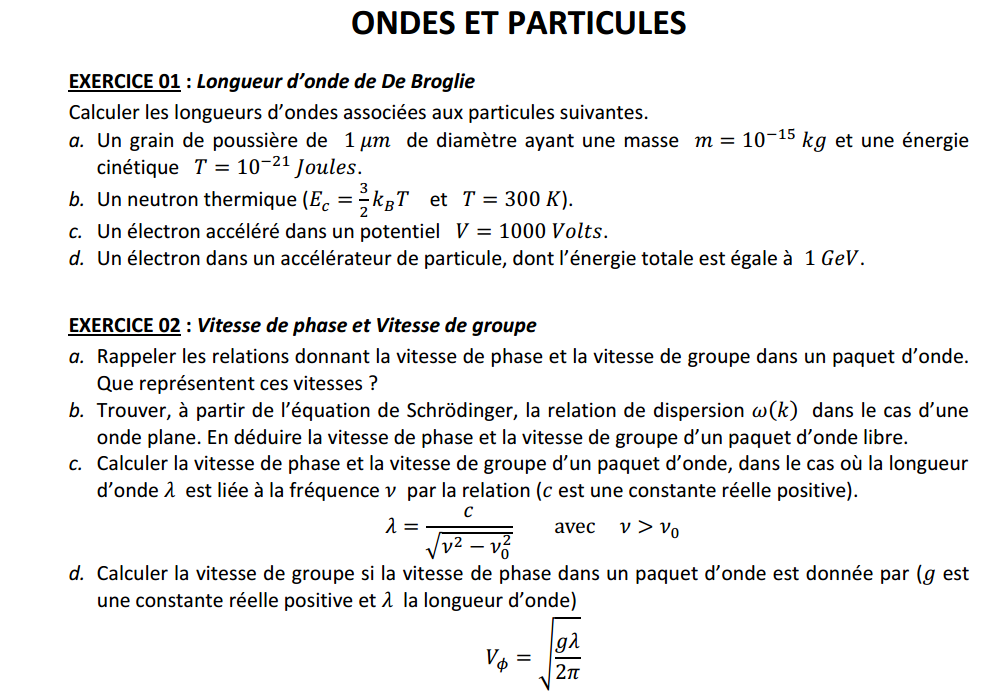
\includegraphics[width=0.9\textwidth]{images/q1.png}
\end{center}
\begin{center}
  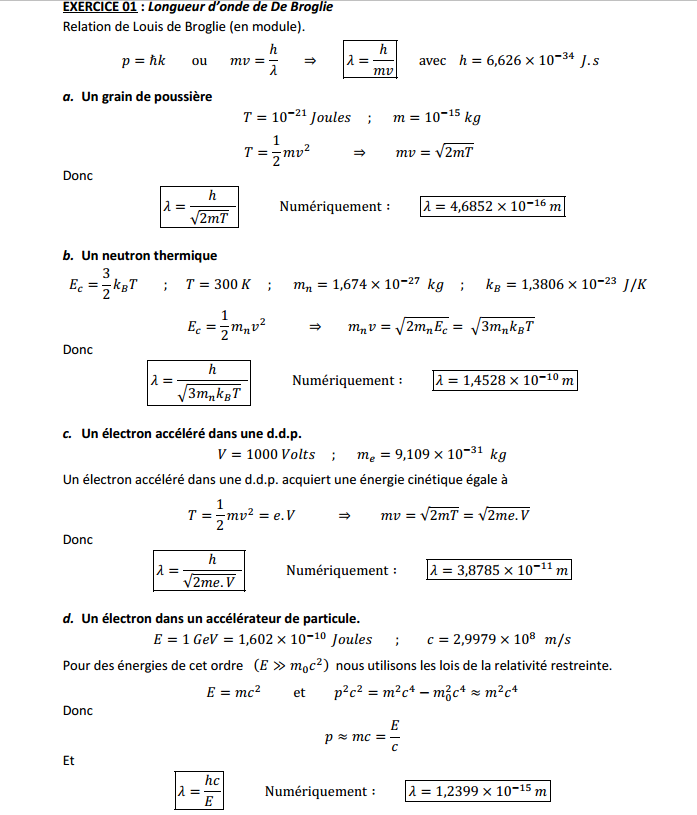
\includegraphics[width=0.9\textwidth]{images/q2.png}
\end{center}
\begin{center}
  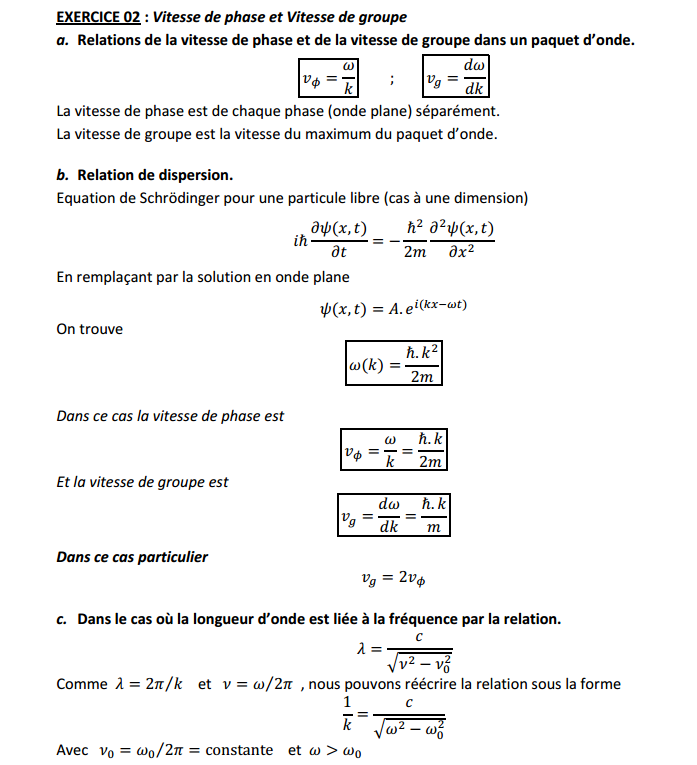
\includegraphics[width=0.9\textwidth]{images/q3.png}
\end{center}
\begin{center}
  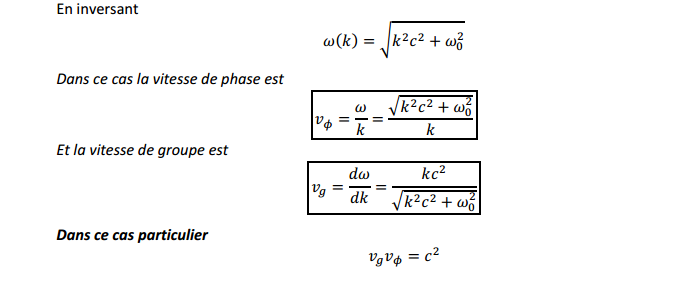
\includegraphics[width=0.9\textwidth]{images/q4.png}
\end{center}
\begin{center}
  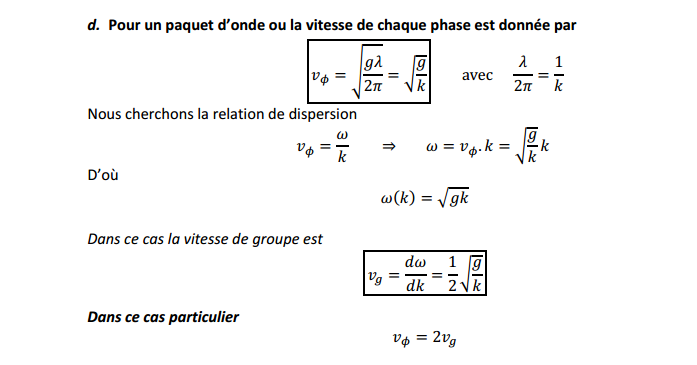
\includegraphics[width=0.9\textwidth]{images/q5.png}
\end{center}
\begin{center}
  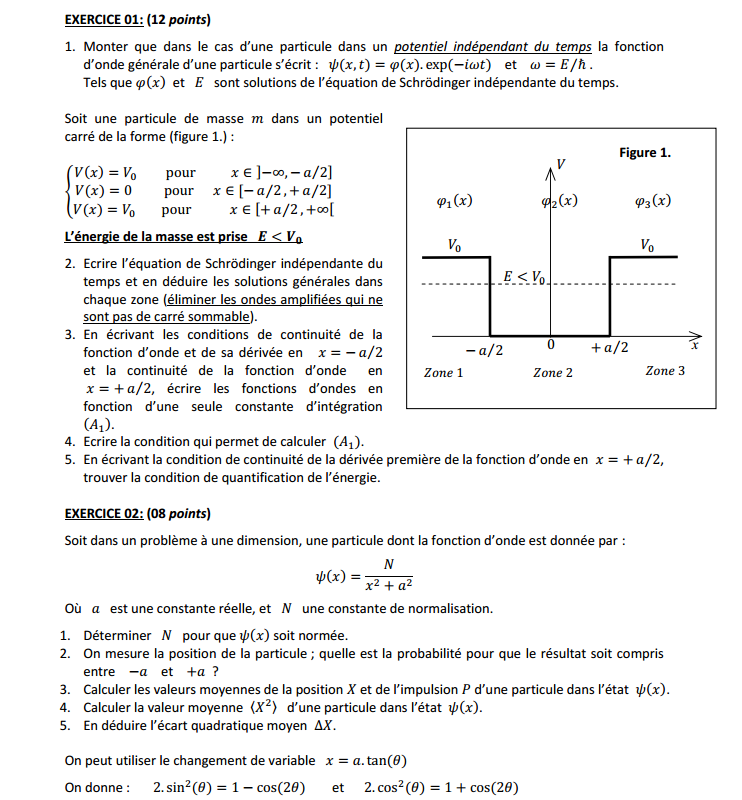
\includegraphics[width=0.9\textwidth]{images/q6.png}
\end{center}
\begin{center}
  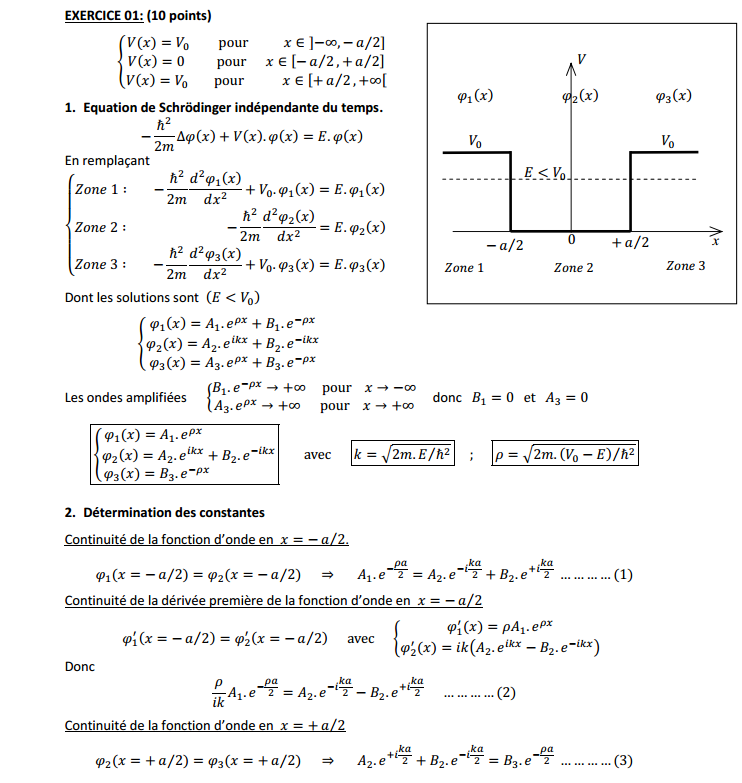
\includegraphics[width=0.9\textwidth]{images/q7.png}
\end{center}
\begin{center}
  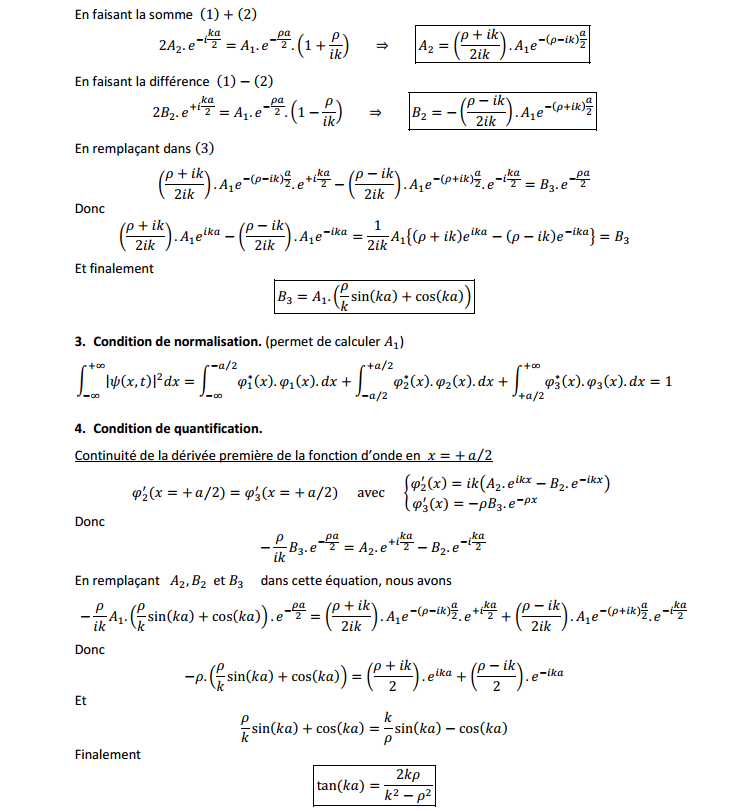
\includegraphics[width=0.9\textwidth]{images/q8.png}
\end{center}

Où $k = \sqrt{2mE/\hbar^2}$ et $\rho = \sqrt{2m(V_0-E)/\hbar^2}$.

\begin{center}
  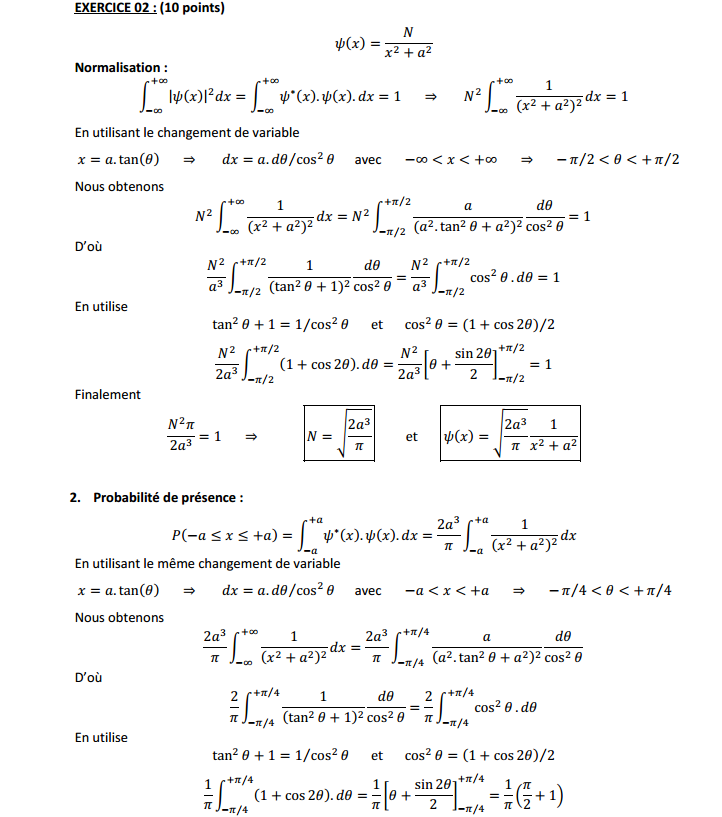
\includegraphics[width=0.9\textwidth]{images/q9.png}
\end{center}
\begin{center}
  
\includegraphics[width=0.9\textwidth]{images/q10.png}
\end{center}
\begin{center}
  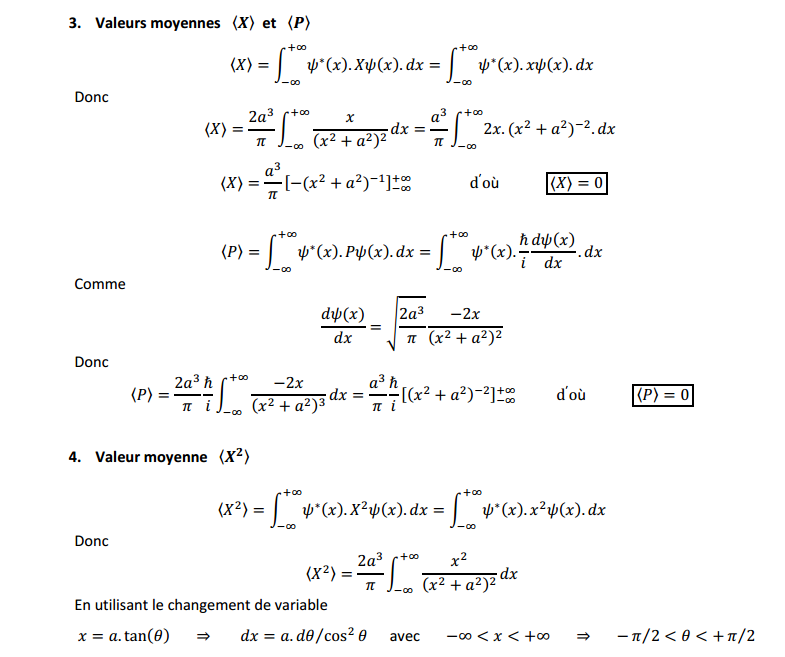
\includegraphics[width=0.9\textwidth]{images/q11.png}
\end{center}
\begin{center}
  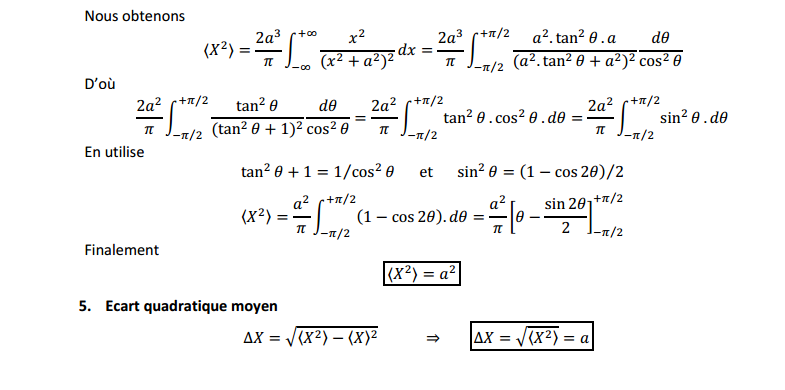
\includegraphics[width=0.9\textwidth]{images/q12.png}
\end{center}
\end{boitecorrige}

\ifdefined\inMainDoc\else\end{document}\fi


% ================================================================
%  UE 6 : MÉCANIQUE DU SOLIDE
% ================================================================
\newpage
\thispagestyle{empty}
\begin{tikzpicture}[remember picture, overlay]
  \fill[gray!12] ([xshift=1.5cm, yshift=3cm]current page.south west)
    rectangle ([xshift=-1.5cm, yshift=-3cm]current page.north east);
  \draw[line width=3pt] ([xshift=1.5cm,yshift=-3cm]current page.north west)
    -- ([xshift=-1.5cm,yshift=-3cm]current page.north east);
  \draw[line width=3pt] ([xshift=1.5cm,yshift=3cm]current page.south west)
    -- ([xshift=-1.5cm,yshift=3cm]current page.south east);
  \node[align=center] at (current page.center) {%
    {\fontsize{30}{38}\bfseries\selectfont MÉCANIQUE DU SOLIDE}\\[1.2cm]
    {\large\itshape Cinématique du solide indéformable}\\[0.4cm]
    {\large\itshape Tenseur d'inertie - Équations d'Euler}\\[1.8cm]
    {\normalsize Licence 2 - UE 6}
  };
  \node[anchor=south west] at ([xshift=2cm,yshift=2cm]current page.south west)
    {\large\bfseries UE 6};
\end{tikzpicture}
\newpage

\addcontentsline{toc}{section}{MÉCANIQUE DU SOLIDE}
\ifdefined\inMainDoc\else
\documentclass[12pt,a4paper]{article}
% ================================================================
%  PRÉAMBULE COMMUN - ANNALES CORRIGÉES
%  Université de Kara - FaST - Licence Fondamentale MPC
%  Design optimisé impression noir et blanc
% ================================================================

% -- ENCODAGE & LANGUE --
\usepackage[utf8]{inputenc}
\usepackage[T1]{fontenc}
\usepackage[french]{babel}
\usepackage{lmodern}
\usepackage{microtype}

% -- MISE EN PAGE --
\usepackage[a4paper, top=2.8cm, bottom=2.5cm, left=2.5cm, right=2.5cm, headheight=14pt]{geometry}
\usepackage{setspace}
\setstretch{1.2}
\usepackage{parskip}
\setlength{\parindent}{1.2em}
\setlength{\parskip}{4pt}

% -- MATHS --
\usepackage{amsmath, amssymb, mathtools, amsthm}
\usepackage{mathrsfs}
\usepackage{dsfont}
\usepackage{bm}
\usepackage{cancel}
\usepackage{textcomp}
% Définition de \oiint (intégrale de surface fermée) sans package supplémentaire
\newcommand{\oiint}{\mathop{\iint\!\!\!\!\!\!\!\bigcirc}\limits}

% -- PHYSIQUE & CHIMIE --
\usepackage{physics}
\usepackage{siunitx}
% Lorsque physics est chargé, siunitx omet \qty. On le restaure ici :
\AtBeginDocument{\RenewCommandCopy\qty\SI}
\sisetup{locale = FR, detect-all, output-decimal-marker={,}}
% Commande de substitution pour les unités posant problème avec pdflatex
% (ohm, degreeCelsius, micro, angstrom, percent utilisent des caractères non-ASCII)
\newcommand{\qtyohm}[1]{\ensuremath{\num{#1}\,\Omega}}
\newcommand{\qtydegc}[1]{\ensuremath{\num{#1}\,{}^\circ\text{C}}}
\newcommand{\qtyangstrom}[1]{\ensuremath{\num{#1}\,\text{\AA}}}
\newcommand{\qtypercent}[1]{\ensuremath{\num{#1}\,\%}}
\newcommand{\qtyum}[1]{\ensuremath{\num{#1}\,\mu\text{m}}}
\usepackage[version=4]{mhchem}

% -- GRAPHISMES --
\usepackage{graphicx}
\usepackage{float}
\usepackage{caption}
\usepackage{subcaption}
\usepackage{wrapfig}
\usepackage{tikz}
\usetikzlibrary{calc, arrows.meta, patterns, shapes.geometric}
\usepackage{pgfplots}
\pgfplotsset{compat=1.18}

% -- TABLEAUX --
\usepackage{booktabs}
\usepackage{array}
\usepackage{tabularx}
\usepackage{multirow}

% -- LISTES --
\usepackage{enumitem}
\setlist[enumerate]{topsep=3pt, itemsep=2pt, parsep=0pt}
\setlist[itemize]{topsep=3pt, itemsep=2pt, parsep=0pt, label={.}}

% -- BOÎTES (noir et blanc) --
\usepackage{mdframed}
\usepackage{tcolorbox}
\tcbuselibrary{skins, breakable, theorems}

% Boîte EXERCICE : encadré avec filet épais, fond blanc
\newmdenv[
  linewidth=1.2pt,
  linecolor=black,
  roundcorner=3pt,
  skipabove=10pt,
  skipbelow=6pt,
  innertopmargin=8pt,
  innerbottommargin=8pt,
  innerleftmargin=10pt,
  innerrightmargin=10pt,
  backgroundcolor=white,
  frametitle={\bfseries\small Exercice},
  frametitlealignment=\raggedright,
  frametitleaboveskip=4pt,
  frametitlebelowskip=4pt,
]{boiteexercice}

% Boîte CORRIGÉ : fond gris très clair + filet fin
\newmdenv[
  linewidth=0.6pt,
  linecolor=black,
  leftline=true,
  rightline=false,
  topline=false,
  bottomline=false,
  linecolor=black,
  innerleftmargin=12pt,
  innerrightmargin=8pt,
  innertopmargin=6pt,
  innerbottommargin=6pt,
  backgroundcolor=gray!8,
  skipabove=4pt,
  skipbelow=8pt,
]{boitecorrige}

% Boîte RÉSUMÉ DE COURS : double encadré
\newmdenv[
  linewidth=0.8pt,
  linecolor=black,
  roundcorner=2pt,
  backgroundcolor=gray!12,
  innertopmargin=10pt,
  innerbottommargin=10pt,
  innerleftmargin=12pt,
  innerrightmargin=12pt,
  skipabove=12pt,
  skipbelow=8pt,
]{boiteresume}

% Boîte ATTENTION/REMARQUE : barre gauche épaisse
\newmdenv[
  leftline=true,
  rightline=false,
  topline=false,
  bottomline=false,
  linewidth=3pt,
  linecolor=black,
  backgroundcolor=gray!5,
  innerleftmargin=12pt,
  innerrightmargin=8pt,
  innertopmargin=5pt,
  innerbottommargin=5pt,
  skipabove=6pt,
  skipbelow=6pt,
]{boiteremarque}

% -- DIFFICULTÉ DES EXERCICES --
\newcommand{\facile}{$\star$}
\newcommand{\moyen}{$\star\!\star$}
\newcommand{\difficile}{$\star\!\star\!\star$}
\newcommand{\niveau}[1]{\hfill\textbf{#1}\hspace{2pt}}

% -- EN-TÊTES ET PIEDS DE PAGE --
\usepackage{fancyhdr}
\pagestyle{fancy}
\fancyhf{}
\renewcommand{\headrulewidth}{0.5pt}
\renewcommand{\footrulewidth}{0.3pt}

% -- HYPERLIENS --
\usepackage[hidelinks]{hyperref}
\hypersetup{
    colorlinks=false,
    pdftitle={Annale Corrigée - Licence MPC - Université de Kara}
}

% -- TITRES --
\usepackage{titlesec}
\titleformat{\section}{\Large\bfseries}{\thesection.}{0.8em}{}[\vspace{2pt}\hrule\vspace{4pt}]
\titleformat{\subsection}{\large\bfseries}{\thesubsection.}{0.7em}{}
\titleformat{\subsubsection}{\normalsize\bfseries}{\thesubsubsection.}{0.6em}{}

% -- THÉORÈMES --
\theoremstyle{definition}
\newtheorem{defn}{Définition}[section]
\newtheorem{prop}{Propriété}[section]
\newtheorem{thm}{Théorème}[section]
\newtheorem{corol}{Corollaire}[section]
\newtheorem{exemple}{Exemple}[section]

% -- COMMANDES MATHÉMATIQUES UTILES --
\newcommand{\vect}[1]{\overrightarrow{#1}}
\newcommand{\R}{\mathbb{R}}
\newcommand{\N}{\mathbb{N}}
\newcommand{\Z}{\mathbb{Z}}
\newcommand{\C}{\mathbb{C}}
\renewcommand{\d}{\mathrm{d}}
\newcommand{\deriv}[2]{\dfrac{\d #1}{\d #2}}
\newcommand{\dpart}[2]{\dfrac{\partial #1}{\partial #2}}
\newcommand{\rot}{\overrightarrow{\mathrm{rot}}\,}
\renewcommand{\div}{\mathrm{div}\,}
\renewcommand{\grad}{\overrightarrow{\mathrm{grad}}\,}
\newcommand{\e}{\mathrm{e}}
\newcommand{\ii}{\mathrm{i}}
\renewcommand{\Tr}{\mathrm{Tr}}

% Numérotation des équations par section
\numberwithin{equation}{section}

% -- RÉSULTATS ENCADRÉS --
\newcommand{\res}[1]{\[\boxed{#1}\]}

% -- REMARQUE INLINE --
\newcommand{\rmq}[1]{\begin{boiteremarque}\textbf{Remarque.} #1\end{boiteremarque}}

% -- MISE EN VALEUR DU RÉSULTAT FINAL --
\newcommand{\reponse}[1]{%
  \begin{center}
    \fbox{\begin{minipage}{0.92\textwidth}\centering #1\end{minipage}}
  \end{center}%
}


% En-têtes et pieds de page
\lhead{\textbf{Mécanique du Solide} - Licence 2}
\rhead{Université de Kara - FaST}
\cfoot{\thepage}
\lfoot{\textit{Licence Fondamentale MPC}}
\rfoot{\textit{Annales corrigées}}

\begin{document}
\fi

\begin{center}
  {\LARGE\bfseries Mécanique du Solide}\\[6pt]
  {\large Licence 2 - Mathématiques, Physique, Chimie}\\[4pt]
  {\normalsize Université de Kara - Faculté des Sciences et Techniques}
\end{center}

\vspace{8pt}
\hrule
\vspace{12pt}

% ================================================================
\section{Résumé de cours}
% ================================================================

\begin{boiteresume}
\textbf{1. Torseurs et cinématique du solide}

Un torseur $[T]$ est défini par sa résultante $\vec{R}$ et son moment $\vec{M}_A$ en un point $A$. La loi de transport est :
\[
\vec{M}_B = \vec{M}_A + \overrightarrow{BA} \wedge \vec{R}.
\]

Le \textbf{torseur cinématique} d'un solide $(S)$ par rapport à un repère $(R)$ a pour résultante le vecteur rotation instantané $\vec{\Omega}(S/R)$ et pour moment en $A$ la vitesse $\vec{V}(A \in S/R)$.

Pour deux solides $(S_1)$ et $(S_2)$ et un repère intermédiaire $(R_1)$ :
\[
\vec{\Omega}(S_2/R) = \vec{\Omega}(S_2/R_1) + \vec{\Omega}(R_1/R).
\]

Vitesse d'un point $B$ du solide connaissant la vitesse de $A$ :
\[
\vec{V}(B \in S/R) = \vec{V}(A \in S/R) + \vec{\Omega}(S/R) \wedge \overrightarrow{AB}.
\]

\medskip
\textbf{2. Centre de masse}

\[
\overrightarrow{OG} = \frac{1}{M}\int \overrightarrow{OM}\,\mathrm{d}m, \qquad M = \int \mathrm{d}m.
\]
Pour un système discret : $\overrightarrow{OG} = \dfrac{1}{M}\sum m_i\,\overrightarrow{OM_i}$.

\medskip
\textbf{3. Moment d'inertie - Théorème de Huygens-Steiner}

Le moment d'inertie d'un solide par rapport à un axe $\Delta$ passant par $G$ vaut $I_G$. Par rapport à un axe $\Delta'$ parallèle à $\Delta$ et distant de $d$ :
\[
I_{\Delta'} = I_G + M\,d^2.
\]

Moments d'inertie usuels (solide de masse $M$) :
\begin{itemize}
  \item Tige de longueur $2\ell$ par rapport au centre : $I_G = \dfrac{M\ell^2}{3}$.
  \item Disque de rayon $R$ par rapport à son axe : $I = \dfrac{MR^2}{2}$.
  \item Sphère pleine de rayon $R$ par rapport à un diamètre : $I = \dfrac{2MR^2}{5}$.
\end{itemize}

\medskip
\textbf{4. Théorème du moment cinétique pour un solide}

Le moment cinétique en $G$ : $\vec{\sigma}(G, S/R) = [I_G]\,\vec{\Omega}(S/R)$ (avec $[I_G]$ tenseur d'inertie).

Pour un mouvement de rotation autour d'un axe fixe $\Delta$ :
\[
\frac{\mathrm{d}}{\mathrm{d}t}\bigl(I_\Delta\,\dot{\theta}\bigr) = \sum \mathcal{M}_\Delta(\vec{F}_{\mathrm{ext}}).
\]

\medskip
\textbf{5. Énergie cinétique - Théorème de Koenig}

\[
E_c(S/R) = \frac{1}{2}M\,\vec{V}^2(G/R) + \frac{1}{2}I_G\,\omega^2 \quad \text{(mouvement plan).}
\]

Plus généralement : $E_c = \dfrac{1}{2}M V_G^2 + \dfrac{1}{2}\vec{\Omega}\cdot\vec{\sigma}(G)$.

Le théorème de l'énergie cinétique : $\dfrac{\mathrm{d}E_c}{\mathrm{d}t} = \mathcal{P}(\vec{F}_{\mathrm{ext}})$.

\medskip
\textbf{6. Liaisons mécaniques courantes}

\begin{itemize}
  \item \textbf{Pivot} (axe $z$) : un seul degré de liberté en rotation $\dot{\theta}$.
  \item \textbf{Glissière} (axe $x$) : un seul degré de liberté en translation $\dot{x}$.
  \item \textbf{Pivot-glissant} (axe $z$) : rotation $\dot{\theta}$ et translation $\dot{z}$ autour et le long du même axe.
  \item \textbf{Rotule} : 3 degrés de liberté en rotation, aucune translation.
\end{itemize}

\medskip
\textbf{7. Équilibre d'un solide - Conditions de Dirichlet}

Un solide est en équilibre si et seulement si la résultante et le moment résultant de toutes les forces extérieures sont nuls :
\[
\sum \vec{F}_i = \vec{0}, \qquad \sum \vec{M}_A(\vec{F}_i) = \vec{0}.
\]
\end{boiteresume}

% ================================================================
\section{Exercices corrigés}
% ================================================================

% ----------------------
\begin{boiteexercice}
\textbf{Exercice 1 - Application antisymétrique et vecteur de rotation}\niveau{\moyen}

Soit $L$ une application de l'espace vectoriel $E$ dans lui-même, définie par :
\[
L(\vec{u}) = \begin{pmatrix} \beta x - y + 4z \\ x + \beta y + \gamma z \\ -\alpha^2 x - y + \beta z \end{pmatrix}
\quad \text{avec } \vec{u} = \begin{pmatrix} x \\ y \\ z \end{pmatrix}.
\]
\begin{enumerate}
  \item Pour quelles valeurs de $\alpha$, $\beta$, $\gamma$ l'application $L$ est-elle antisymétrique ?
  \item Montrer qu'il existe un vecteur $\vec{\Omega}$ tel que $L(\vec{u}) = \vec{\Omega} \wedge \vec{u}$, et déterminer $\vec{\Omega}$.
\end{enumerate}
\end{boiteexercice}

\begin{boitecorrige}
\textbf{1.} $L$ est antisymétrique si et seulement si sa matrice $\mathbf{L}$ vérifie $\mathbf{L}^T = -\mathbf{L}$, ce qui impose des éléments diagonaux nuls et une antisymétrie des éléments hors diagonaux.

La matrice associée à $L$ dans la base $(\vec{i}, \vec{j}, \vec{k})$ est :
\[
\mathbf{L} = \begin{pmatrix} \beta & -1 & 4 \\ 1 & \beta & \gamma \\ -\alpha^2 & -1 & \beta \end{pmatrix}.
\]

Condition $\mathbf{L}^T = -\mathbf{L}$ :
\[
\begin{cases} \beta = 0 & \text{(diagonale nulle)} \\ \gamma + 4 = 0 \Rightarrow \gamma = -4 & (\text{mais on lit ici : vérification ligne par ligne}) \end{cases}
\]

Plus précisément, $L_{12} = -1$ et $L_{21} = 1$ donnent bien $L_{12} = -L_{21}$ : condition satisfaite. $L_{13} = 4$ et $L_{31} = -\alpha^2$ donnent $-\alpha^2 = -4$, soit $\alpha^2 = 4$, c'est-à-dire $\alpha = \pm 2$. $L_{23} = \gamma$ et $L_{32} = -1$ donnent $\gamma = 1$. La diagonale impose $\beta = 0$.

Ainsi : $\beta = 0$, $\gamma = 1$, $\alpha = \pm 2$, et :
\[
\mathbf{L} = \begin{pmatrix} 0 & -1 & 4 \\ 1 & 0 & 1 \\ -4 & -1 & 0 \end{pmatrix}.
\]

\textbf{2.} Pour une matrice antisymétrique $3 \times 3$, il existe toujours $\vec{\Omega} = (a, b, c)^T$ tel que $L(\vec{u}) = \vec{\Omega} \wedge \vec{u}$.

\[
\vec{\Omega} \wedge \vec{u} = \begin{pmatrix} bz - cy \\ cx - az \\ ay - bx \end{pmatrix}.
\]

En identifiant avec $L(\vec{u}) = \begin{pmatrix} -y + 4z \\ x + z \\ -4x - y \end{pmatrix}$, on obtient :
\[
\begin{cases} b = 4, \quad c = 1 \\ c = 1, \quad a = -1 \\ a = -1, \quad b = 4 \end{cases}
\quad \Rightarrow \quad \vec{\Omega} = \begin{pmatrix} -1 \\ 4 \\ 1 \end{pmatrix}.
\]

\begin{center}
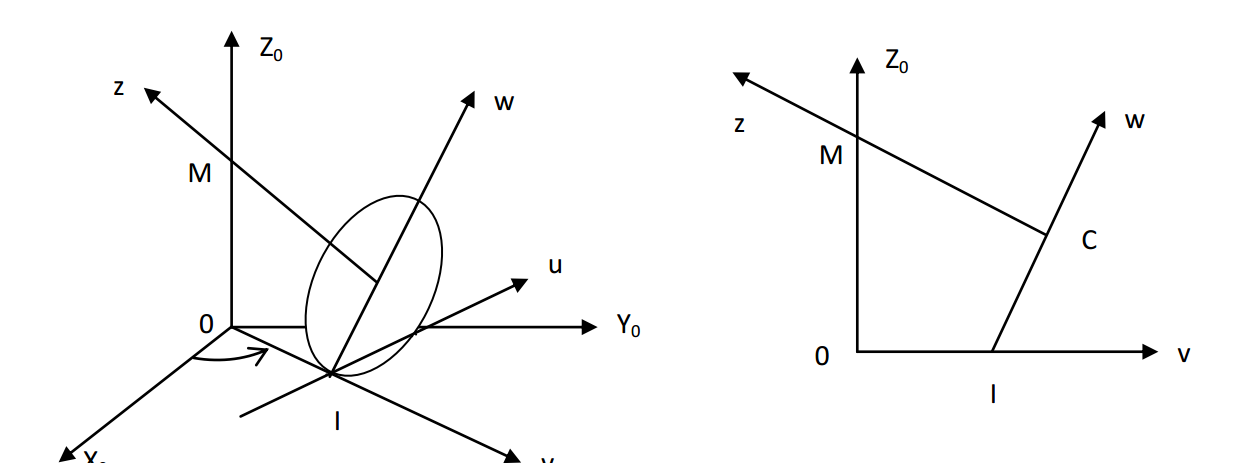
\includegraphics[width=0.45\textwidth]{images/mecanique_solide/ms-006-004.png}\\[4pt]
{\small\itshape Application linéaire antisymétrique $L(\vec{u}) = \vec{\Omega}\wedge\vec{u}$ : repérage du vecteur rotation $\vec{\Omega}$.}
\end{center}
\end{boitecorrige}

% ----------------------
\begin{boiteexercice}
\textbf{Exercice 2 - Torseurs cinématiques : disque en rotation}\niveau{\facile}

Dans un repère $R(O, \vec{i}, \vec{j}, \vec{k})$, un disque de centre $O$ contenu dans le plan $xOy$ tourne dans le sens trigonométrique autour de $Oz$ avec une vitesse angulaire $\omega$.

\begin{enumerate}
  \item Déterminer la vitesse $\vec{V}(M/R)$ d'un point $M(x, y, 0)$ du disque.
  \item Montrer que le champ $\vec{V}(M/R)$ est un torseur et en déterminer les éléments de réduction en $O$.
  \item De quel type de torseur s'agit-il ? Quel est son axe central ?
\end{enumerate}
\end{boiteexercice}

\begin{boitecorrige}
\textbf{1.} Le vecteur rotation du disque est $\vec{\Omega} = \omega\,\vec{k}$. La vitesse de $M$ est :
\[
\vec{V}(M/R) = \vec{\Omega} \wedge \overrightarrow{OM} = \omega\vec{k} \wedge (x\vec{i}+y\vec{j}) = \omega(-y\vec{i} + x\vec{j}).
\]

\textbf{2.} Vérifions que le champ est équiprojectif : pour deux points $M$ et $M'$,
\[
\overrightarrow{MM'} \cdot \bigl(\vec{V}(M) - \vec{V}(M')\bigr) = \overrightarrow{MM'} \cdot \bigl[\vec{\Omega} \wedge \overrightarrow{MM'}\bigr] = 0,
\]
car le produit scalaire d'un vecteur par son produit vectoriel avec un autre est nul. Le champ est donc équiprojectif, ce qui en fait un torseur.

Éléments de réduction en $O$ : la résultante est $\vec{R} = \vec{\Omega} = \omega\vec{k}$ et le moment en $O$ est $\vec{V}(O/R) = \vec{0}$.

Les éléments de réduction sont $[V]_O = [\vec{0},\, \omega\vec{k}]$.

\begin{center}

\includegraphics[width=0.45\textwidth]{images/mecanique_solide/ms-006-005.png}\\[4pt]
{\small\itshape Disque en rotation autour de l'axe $Oz$ : vitesse $\vec{V}(M) = \vec{\Omega}\wedge\overrightarrow{OM}$ et équiprojectivité du champ des vitesses.}
\end{center}

\textbf{3.} L'invariant scalaire est $I = \vec{R} \cdot \vec{M}_O = \omega\vec{k} \cdot \vec{0} = 0$. C'est un \textbf{glisseur}. Son axe central est la droite passant par $O$ dirigée selon $\vec{k}$, c'est-à-dire l'axe de rotation $Oz$.
\end{boitecorrige}

% ----------------------
\begin{boiteexercice}
\textbf{Exercice 3 - Centre de masse de solides usuels}\niveau{\moyen}

Déterminer les coordonnées du centre d'inertie $G$ des solides suivants :
\begin{enumerate}
  \item Un arc de cercle homogène de centre $O$, de rayon $R$, de densité linéique $\lambda$, vu sous un angle $2\alpha$ de part et d'autre de l'axe $Ox$.
  \item Une plaque triangulaire homogène de densité surfacique $\sigma$, formant le triangle $OAB$ avec $\overrightarrow{OA} = a\vec{x}$ et $\overrightarrow{OB} = b\vec{y}$.
  \item Une demi-sphère pleine homogène de centre $O$, de rayon $R$, d'axe de symétrie $Oz$, de densité $\rho$.
\end{enumerate}
\end{boiteexercice}

\begin{boitecorrige}
\textbf{1. Arc de cercle.}

Par symétrie par rapport à $Ox$, on a $y_G = z_G = 0$. En paramétrant l'arc par l'angle $\varphi \in [-\alpha, \alpha]$ :
\[
x_G = \frac{\displaystyle\int_{-\alpha}^{\alpha} R\cos\varphi\,\lambda R\,\mathrm{d}\varphi}
           {\displaystyle\int_{-\alpha}^{\alpha} \lambda R\,\mathrm{d}\varphi}
= R\,\frac{\bigl[\sin\varphi\bigr]_{-\alpha}^{\alpha}}{2\alpha}
= R\,\frac{\sin\alpha}{\alpha}.
\]

\begin{center}
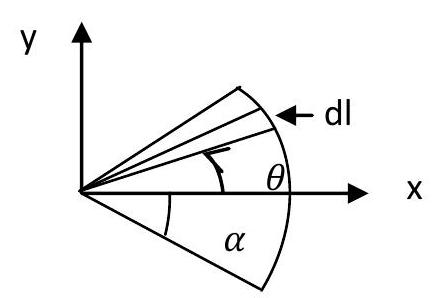
\includegraphics[width=0.45\textwidth]{images/mecanique_solide/ms-008-008.png}\\[4pt]
{\small\itshape Arc de cercle vu sous un angle $2\alpha$ : élément $\mathrm{d}\ell = R\,\mathrm{d}\theta$.}
\end{center}

\textbf{2. Plaque triangulaire.}

La masse totale est $m = \sigma\,\dfrac{ab}{2}$. L'équation de $AB$ est $y = -\dfrac{b}{a}x + b$.

Pour $x_G$ : élément de surface $\mathrm{d}s = y\,\mathrm{d}x$ avec $0 \leq x \leq a$.
\[
x_G = \frac{1}{m}\int_0^a x\sigma y\,\mathrm{d}x = \frac{2\sigma}{ab}\int_0^a x\!\left(-\frac{b}{a}x+b\right)\mathrm{d}x
= \frac{2}{a}\!\left[-\frac{x^3}{3a}+\frac{x^2}{2}\right]_0^a = \frac{2}{a}\cdot\frac{a^2}{6} = \frac{a}{3}.
\]

De même : $y_G = \dfrac{b}{3}$. Le centre de masse du triangle est donc au tiers de chaque côté depuis l'origine.

\begin{center}
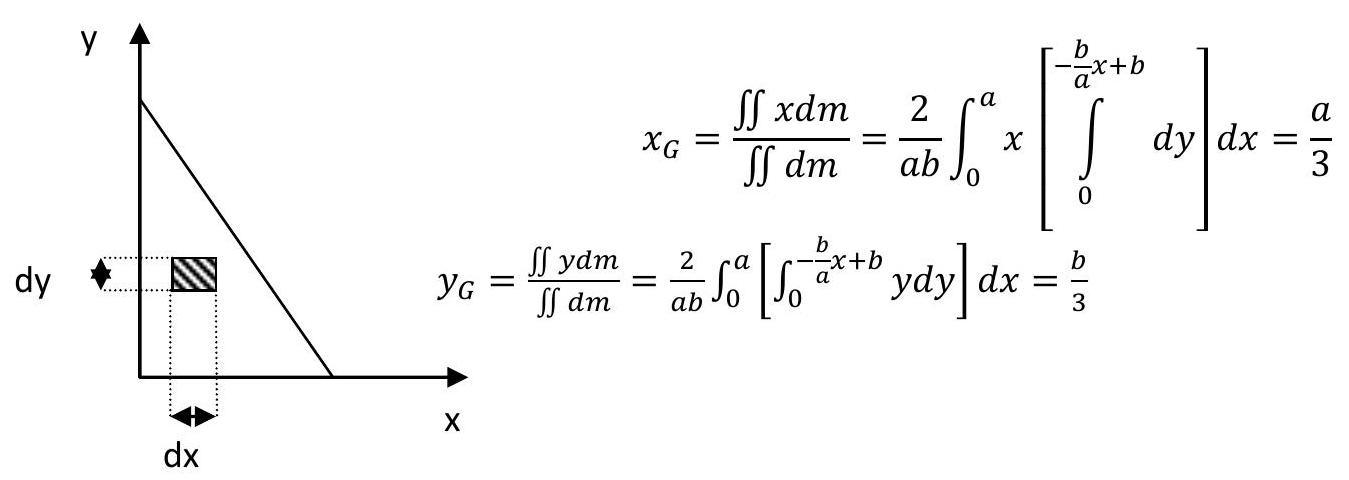
\includegraphics[width=0.45\textwidth]{images/mecanique_solide/ms-009-009.png}\quad
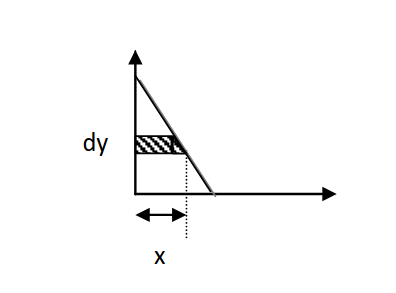
\includegraphics[width=0.40\textwidth]{images/mecanique_solide/ms-009-011.png}\\[4pt]
{\small\itshape Plaque triangulaire : coordonnées du centre de gravité $G(a/3, b/3)$ et élément de surface.}
\end{center}

\begin{center}
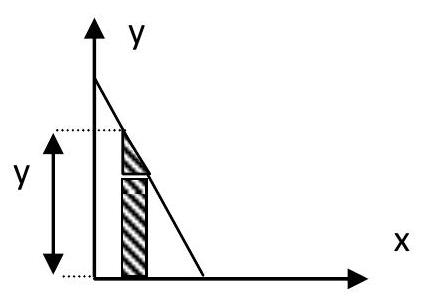
\includegraphics[width=0.45\textwidth]{images/mecanique_solide/ms-009-010.png}\quad

\includegraphics[width=0.40\textwidth]{images/mecanique_solide/ms-009-012.png}\\[4pt]
{\small\itshape Autres vues de la plaque triangulaire : décomposition de l'élément de surface $\d s = y\,\d x$ et intégration sur le domaine $OAB$.}
\end{center}

\textbf{3. Demi-sphère.}

Par symétrie, $x_G = y_G = 0$. En coordonnées sphériques $(r, \theta, \varphi)$ avec $\theta \in [0, \pi/2]$, $r \in [0, R]$ :
\[
z_G = \frac{\displaystyle\int_0^R\!\int_0^{\pi/2}\!\int_0^{2\pi} r\cos\theta \cdot \rho r^2\sin\theta\,\mathrm{d}r\,\mathrm{d}\theta\,\mathrm{d}\varphi}
           {\displaystyle\int_0^R\!\int_0^{\pi/2}\!\int_0^{2\pi} \rho r^2\sin\theta\,\mathrm{d}r\,\mathrm{d}\theta\,\mathrm{d}\varphi}.
\]

Numérateur : $\rho \cdot \dfrac{R^4}{4} \cdot \dfrac{1}{2} \cdot 2\pi = \dfrac{\pi\rho R^4}{4}$.

Dénominateur : $\rho \cdot \dfrac{R^3}{3} \cdot 1 \cdot 2\pi = \dfrac{2\pi\rho R^3}{3}$.

\[
z_G = \frac{\pi\rho R^4/4}{2\pi\rho R^3/3} = \frac{R}{4} \cdot \frac{3}{2} = \frac{3R}{8}.
\]

\begin{center}
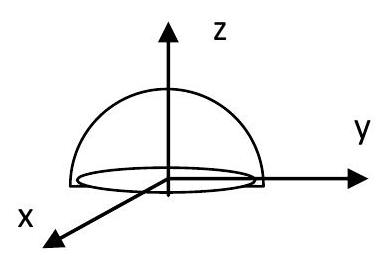
\includegraphics[width=0.40\textwidth]{images/mecanique_solide/ms-010-013.png}\\[4pt]
{\small\itshape Demi-sphère pleine de rayon $R$ : le centre de masse est à $z_G = 3R/8$ de la base.}
\end{center}

\textbf{4. Cône plein (exemple complémentaire).}

Pour un cône droit de hauteur $h$ et de rayon de base $R$, en coordonnées cylindriques :
\[
z_G = \frac{\displaystyle\int_0^h z\,\rho\pi\!\left(R(1-z/h)\right)^2\mathrm{d}z}
           {\displaystyle\int_0^h \rho\pi\!\left(R(1-z/h)\right)^2\mathrm{d}z}
       = \frac{3h}{4}.
\]

\begin{center}
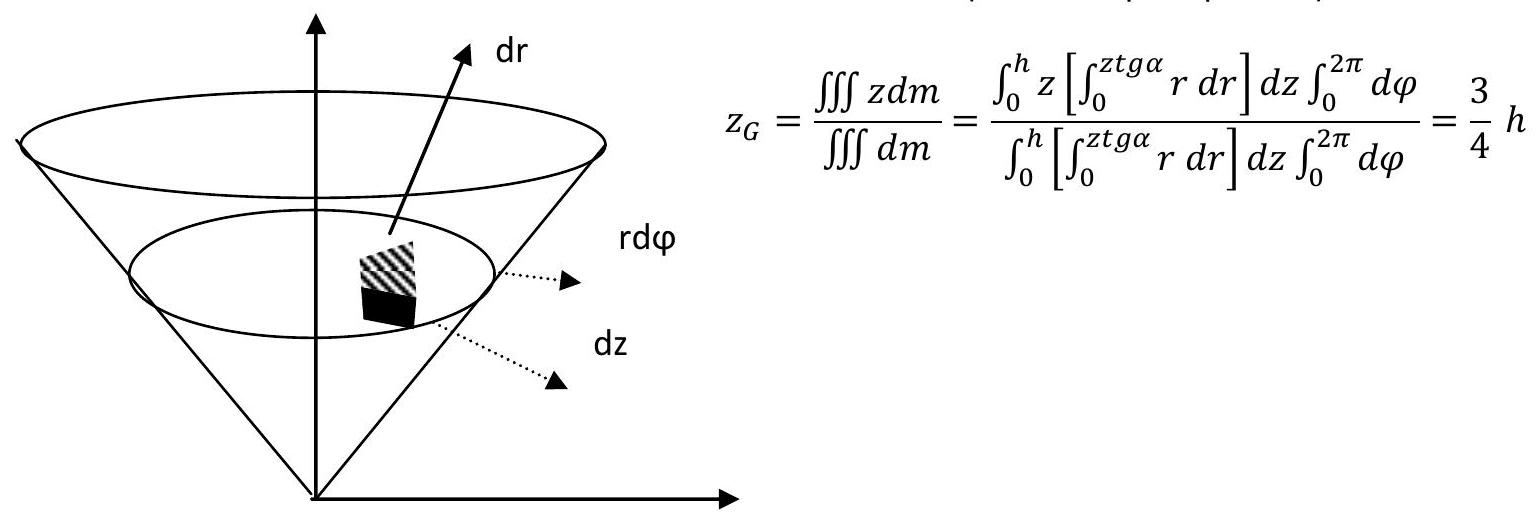
\includegraphics[width=0.40\textwidth]{images/mecanique_solide/ms-010-014.png}\\[4pt]
{\small\itshape Cône de hauteur $h$ : élément de volume et centre de masse $z_G = 3h/4$.}
\end{center}
\end{boitecorrige}

% ----------------------
\begin{boiteexercice}
\textbf{Exercice 4 - Disque sur tapis roulant incliné (dynamique)}\niveau{\difficile}

Un disque homogène de masse $m$, de rayon $r$, de centre $G$, est posé sans vitesse initiale sur un tapis roulant incliné d'un angle $\alpha$ se déplaçant à la vitesse constante $v_0\,\vec{i}_0$ (avec $v_0 > 0$). La réaction de contact est $\vec{R} = T\vec{i}_0 + N\vec{j}_0$ avec $|T| = fN$ tant qu'il y a glissement.

On pose $\overrightarrow{OG} = x_G\vec{i}_0 + r\vec{j}_0$.

\begin{enumerate}
  \item Calculer la vitesse de glissement initiale du disque sur le tapis.
  \item Appliquer le principe fondamental de la dynamique et obtenir les équations du mouvement.
  \item Calculer la dérivée par rapport au temps de la vitesse de glissement.
  \item Décrire l'évolution de la vitesse de glissement selon les valeurs de $f$ et $\alpha$.
\end{enumerate}
\end{boiteexercice}

\begin{boitecorrige}
\textbf{1. Vitesse de glissement initiale.}

\begin{center}
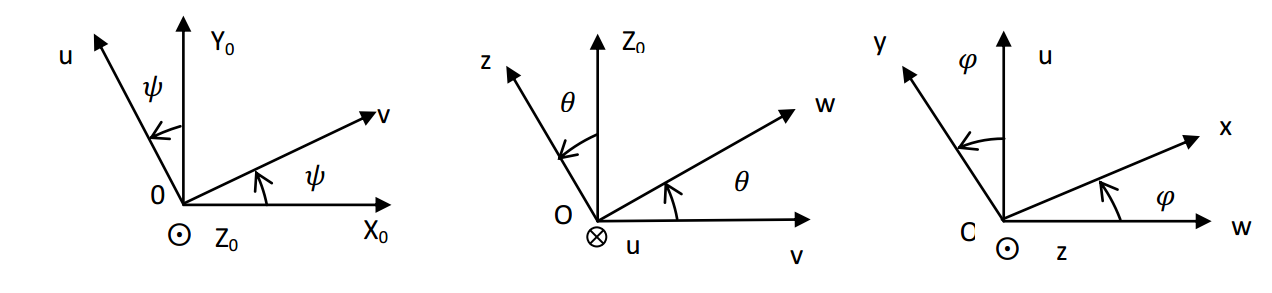
\includegraphics[width=0.50\textwidth]{images/mecanique_solide/ms-006-006.png}\\[4pt]
{\small\itshape Disque posé sur un tapis roulant incliné : repère $(\vec{i}_0, \vec{j}_0)$, angle $\alpha$ et point de contact $I$.}
\end{center}

La vitesse de glissement du disque sur le tapis est :
\[
\vec{v}_g = \vec{V}(I \in S_1/R_0) - \vec{V}(I \in S_2/R_0) = (\dot{x}_G + r\dot{\theta} - v_0)\vec{i}_0.
\]
À $t = 0$, le disque est posé sans vitesse initiale : $\dot{x}_G(0) = 0$, $\dot{\theta}(0) = 0$. Donc :
\[
\vec{v}_{g0} = -v_0\,\vec{i}_0.
\]

\textbf{2. Principe fondamental de la dynamique.}

Théorème de la résultante (projection sur $\vec{i}_0$ et $\vec{j}_0$) :
\[
m\ddot{x}_G = T - mg\sin\alpha, \qquad 0 = N - mg\cos\alpha \Rightarrow N = mg\cos\alpha.
\]

Théorème du moment cinétique en $G$ (moment d'inertie du disque : $I_G = mr^2/2$) :
\[
\frac{mr^2}{2}\,\ddot{\theta} = Tr \quad \Rightarrow \quad \ddot{\theta} = \frac{2T}{mr}.
\]

\textbf{3. Dérivée de la vitesse de glissement.}

\[
\frac{\mathrm{d}v_g}{\mathrm{d}t} = \ddot{x}_G + r\ddot{\theta} = \frac{T}{m} - g\sin\alpha + \frac{2T}{m} = \frac{3T}{m} - g\sin\alpha.
\]

Comme $\vec{v}_{g0} = -v_0\vec{i}_0 < 0$, la force de frottement agit dans le sens de $+\vec{i}_0$ : $T = +fN = fmg\cos\alpha$.

\[
\frac{\mathrm{d}v_g}{\mathrm{d}t} = 3g\cos\alpha\!\left(f - \frac{\tan\alpha}{3}\right).
\]

\textbf{4. Évolution de la vitesse de glissement.}

La vitesse de glissement part de $v_g(0) = -v_0 < 0$.

\begin{itemize}
  \item Si $f > \dfrac{\tan\alpha}{3}$ : $\dfrac{\mathrm{d}v_g}{\mathrm{d}t} > 0$, la vitesse de glissement augmente depuis $-v_0$ jusqu'à $0$. Il y a d'abord glissement, puis roulement pur dès que $v_g = 0$.
  \item Si $f < \dfrac{\tan\alpha}{3}$ : $\dfrac{\mathrm{d}v_g}{\mathrm{d}t} < 0$, la vitesse de glissement décroît à partir de $-v_0$ : il y a toujours glissement.
  \item Si $f = \dfrac{\tan\alpha}{3}$ : la vitesse de glissement reste constante à $-v_0$ ; il y a glissement permanent sans variation.
\end{itemize}
\end{boitecorrige}

% ----------------------
\begin{boiteexercice}
\textbf{Exercice 5 - Roulement d'un cerceau sur un plan}\niveau{\difficile}

Un cerceau $(C_1)$ de rayon $a$, dont le plan est vertical, roule sans glisser sur le plan horizontal $(\pi)$. Le point de contact décrit un cercle de rayon $R$ avec une vitesse angulaire uniforme $\dot{\theta} = \text{cte}$. Soit $R_0(O, \vec{x}_0, \vec{y}_0, \vec{z}_0)$ le repère lié à $(\pi)$ et $R_1(O_1, \vec{x}_1, \vec{y}_1, \vec{z}_0)$ le repère en rotation uniforme autour de $Oz_0$.

\begin{enumerate}
  \item Déterminer $\vec{\Omega}(C_1/R_1)$ et $\vec{\Omega}(C_1/R_0)$.
  \item Calculer les vitesses du point géométrique de contact $I_{G_1}$ et du point matériel $I_1$.
  \item En déduire la condition de roulement sans glissement.
\end{enumerate}
\end{boiteexercice}

\begin{boitecorrige}
\textbf{1. Vecteurs rotation.}

\begin{center}
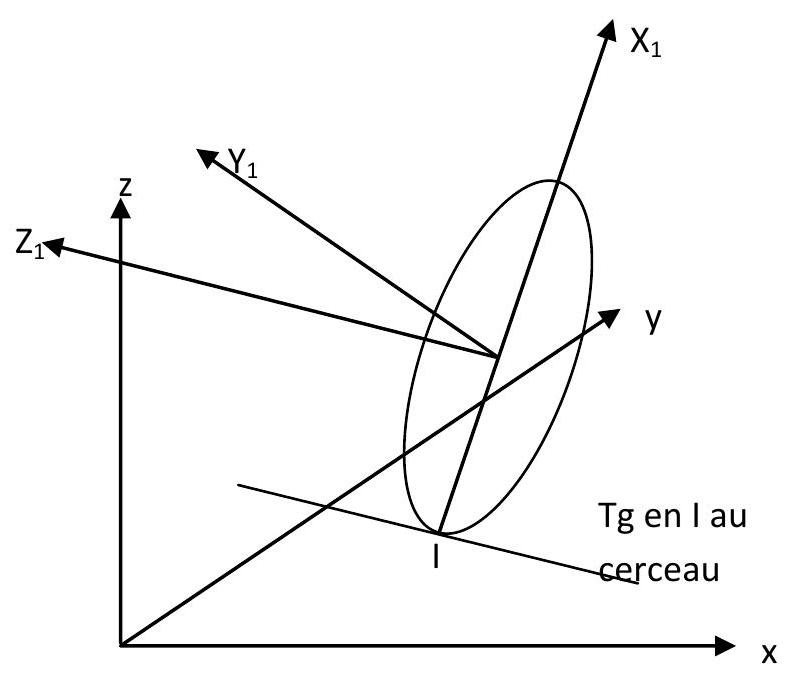
\includegraphics[width=0.55\textwidth]{images/mecanique_solide/ms-003-000.png}\\[4pt]
{\small\itshape Cerceau en contact avec un plan : repère et point de contact $I$.}
\end{center}

\begin{center}

\includegraphics[width=0.50\textwidth]{images/mecanique_solide/ms-006-007.png}\\[4pt]
{\small\itshape Repère $R_1$ en rotation uniforme autour de $Oz_0$ : position du centre $A_1$ et trajectoire circulaire de rayon $R$.}
\end{center}

Le cerceau tourne autour de l'axe $O_1\vec{x}_1$ dans $R_1$ avec une vitesse angulaire $\dot{\varphi}$ :
\[
\vec{\Omega}(C_1/R_1) = \dot{\varphi}\,\vec{x}_1.
\]

Le repère $R_1$ tourne autour de $Oz_0$ à vitesse $\dot{\theta}$ :
\[
\vec{\Omega}(C_1/R_0) = \vec{\Omega}(C_1/R_1) + \vec{\Omega}(R_1/R_0) = \dot{\varphi}\,\vec{x}_1 + \dot{\theta}\,\vec{z}_0.
\]

\textbf{2. Vitesses.}

Le centre $A_1$ du cerceau est à distance $R$ de $O_1$ et suit un mouvement circulaire dans $R_0$ :
\[
\vec{V}(A_1/R_0) = R\dot{\theta}\,\vec{y}_1.
\]

Vitesse du point géométrique de contact $I_{G_1}$ (point de $(\pi)$, donc fixe dans $R_0$... mais $I_{G_1}$ se déplace) :
\[
\vec{V}(I_{G_1}/R_0) = \vec{V}(A_1/R_0) + \vec{\Omega}(C_1/R_0) \wedge \overrightarrow{A_1 I_{G_1}} = R\dot{\theta}\,\vec{y}_1 \quad \Rightarrow \quad \vec{v}(I_{G_1}/R_0) = R\dot{\theta}\,\vec{y}_1.
\]

Vitesse du point matériel $I_1$ appartenant au cerceau :
\[
\vec{V}(I_1/R_0) = \vec{V}(A_1/R_0) + \vec{\Omega}(C_1/R_0) \wedge \overrightarrow{A_1 I_1} = (R\dot{\theta} + a\dot{\varphi})\,\vec{y}_1.
\]

\textbf{3. Condition de roulement sans glissement.}

La condition $\vec{V}(I_1 \in C_1/R_0) = \vec{V}(I_{G_1} \in (\pi)/R_0) = \vec{0}$ (le plan est fixe) donne :
\[
R\dot{\theta} + a\dot{\varphi} = 0 \quad \Rightarrow \quad \dot{\varphi} = -\frac{R}{a}\dot{\theta}.
\]
\end{boitecorrige}

% ----------------------
\begin{boiteexercice}
\textbf{Exercice 6 - Système barre et disque : dynamique plane}\niveau{\difficile}

Un système $(\Sigma)$ est constitué d'une barre $AB$ de longueur $2\ell$, de milieu $G_1$, de masse $m_1$ (solide $S_1$) et d'un disque homogène de centre $C$, de rayon $r$, de masse $m_2$ (solide $S_2$). L'extrémité $A$ de $S_1$ glisse sans frottement sur l'axe $Ox_0$. $S_1$ glisse sur $S_2$ avec un coefficient de frottement $f$. On applique sur $S_2$ un couple $\vec{\Gamma} = -\Gamma\,\vec{k}_0$ ($\Gamma > 0$). La position de $S_1$ est repérée par $(x_A, \varphi)$ et celle de $S_2$ par $(x_C, \theta)$.

\begin{enumerate}
  \item Exprimer $\vec{\Omega}(S_1/R_0)$, $\vec{\Omega}(S_2/R_0)$, $\vec{V}(G_1/R_0)$ et $\vec{\gamma}(C/R_0)$.
  \item Donner la condition de roulement sans glissement de $S_2$ sur $Ox_0$.
  \item Appliquer le théorème du centre de masse à $S_1$ et à $S_2$.
\end{enumerate}
\end{boiteexercice}

\begin{boitecorrige}
\textbf{1. Cinématique.}

\begin{center}
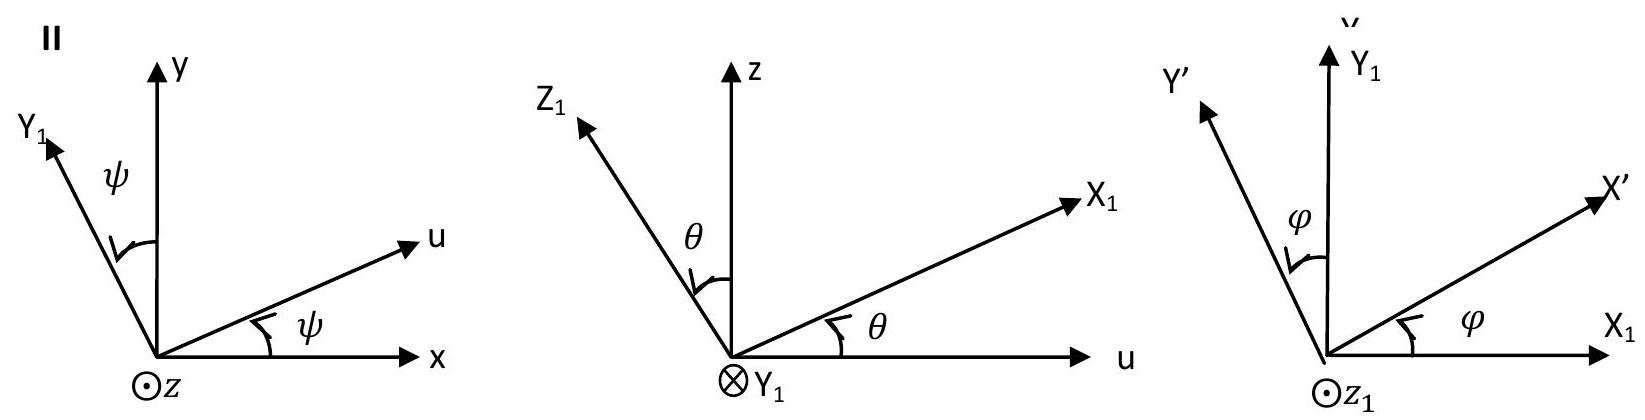
\includegraphics[width=0.45\textwidth]{images/mecanique_solide/ms-004-001.png}\quad
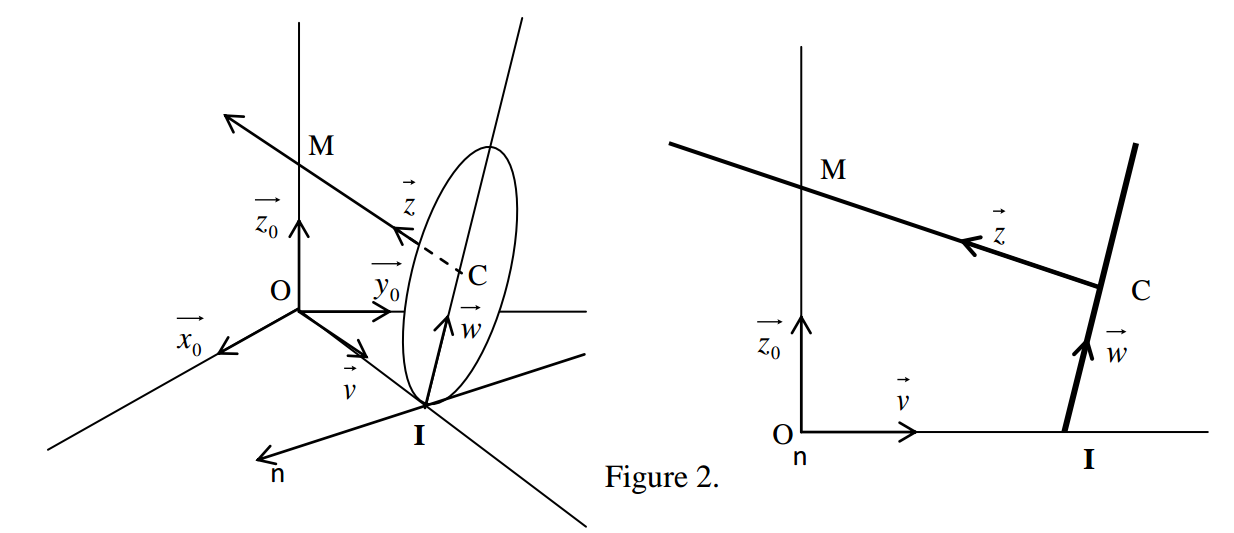
\includegraphics[width=0.45\textwidth]{images/mecanique_solide/ms-005-002.png}\\[4pt]
{\small\itshape Repères d'Euler $(\psi,\theta,\varphi)$ et configuration du système barre--disque (points $O, I, M, C$).}
\end{center}

\begin{center}

\includegraphics[width=0.50\textwidth]{images/mecanique_solide/ms-005-003.png}\\[4pt]
{\small\itshape Schéma complémentaire : repérage angulaire et points caractéristiques du système barre--disque en dynamique plane.}
\end{center}

\[
\vec{\Omega}(S_1/R_0) = \dot{\varphi}\,\vec{k}_0, \qquad \vec{\Omega}(S_2/R_0) = \dot{\theta}\,\vec{k}_0.
\]

Le milieu $G_1$ de $AB$ a pour coordonnées $(x_A + \ell\cos\varphi,\, \ell\sin\varphi, 0)$. Sa vitesse est :
\[
\vec{V}(G_1/R_0) = (\dot{x}_A - \ell\dot{\varphi}\sin\varphi)\,\vec{i}_0 + (\ell\dot{\varphi}\cos\varphi)\,\vec{j}_0.
\]

L'accélération du centre $C$ du disque (mouvement de translation si $S_2$ roule sans glisser) :
\[
\vec{\gamma}(C/R_0) = \ddot{x}_C\,\vec{i}_0 \quad \text{(si roulement pur sur } Ox_0\text{)}.
\]

\textbf{2. Condition de roulement sans glissement.}

Si $S_2$ roule sans glisser sur $Ox_0$, la vitesse du point de contact de $S_2$ avec l'axe est nulle :
\[
\vec{V}(I \in S_2/R_0) = \vec{V}(C/R_0) + \vec{\Omega}(S_2/R_0) \wedge \overrightarrow{CI} = \vec{0}.
\]
Avec $\overrightarrow{CI} = -r\vec{j}_0$ : $\dot{x}_C\vec{i}_0 + \dot{\theta}\vec{k}_0 \wedge (-r\vec{j}_0) = \dot{x}_C\vec{i}_0 + r\dot{\theta}\vec{i}_0 = \vec{0}$, soit $\dot{x}_C = -r\dot{\theta}$.

\textbf{3. Théorème du centre de masse.}

Pour $S_1$ (projection sur $\vec{i}_0$ et $\vec{j}_0$, avec $\vec{R}_A = R_A\vec{j}_0$ la réaction sur $A$, et $\vec{R}_J = T_j\vec{i}_1 + N_j\vec{j}_1$ la réaction de $S_2$ sur $S_1$) :
\[
m_1\ddot{x}_{G_1} = (T_j\cos\varphi - N_j\sin\varphi), \qquad
m_1\ddot{y}_{G_1} = R_A + T_j\sin\varphi + N_j\cos\varphi - m_1 g.
\]

Pour $S_2$ (translation du centre $C$, forces : réaction $\vec{R}_I$ de $Ox_0$ sur $S_2$, réaction de $S_1$ sur $S_2$ $= -\vec{R}_J$, poids $-m_2 g\vec{j}_0$) :
\[
m_2\ddot{x}_C = -T_j\cos\varphi + N_j\sin\varphi + T_i, \qquad
0 = -T_j\sin\varphi - N_j\cos\varphi + N_i - m_2 g.
\]

Le théorème du moment cinétique en $C$ pour $S_2$ :
\[
\frac{m_2 r^2}{2}\,\ddot{\theta} = r T_i - \Gamma + r(-T_j\cos\varphi + N_j\sin\varphi).
\]
\end{boitecorrige}

\subsection*{Exercice 7 - Cerceau roulant sur un plan horizontal \niveau{\difficile}}

\begin{boiteexercice}
Un cerceau $(C_1)$ de rayon $a$, dans un plan vertical, roule sans glisser sur le plan horizontal $(\pi)$. Le point de contact décrit un cercle de rayon $R$ avec vitesse angulaire uniforme $\dot{\theta} = \mathrm{cte}$. On note $R_0(O,\vec{i}_0,\vec{j}_0,\vec{k}_0)$ le repère fixe et $R_1(O_1,\vec{i}_1,\vec{j}_1,\vec{k}_0)$ le repère en rotation autour de $O\vec{k}_0$.
\begin{enumerate}
  \item Déterminer $\vec{\Omega}(C_1/R_1)$ et $\vec{\Omega}(C_1/R_0)$.
  \item Calculer $\vec{v}(I_{G_1}/R_0)$ et $\vec{v}(I_1/R_0)$. En déduire la condition de roulement sans glissement.
  \item Calculer $\vec{\gamma}(I_{G_1}/R_0)$ et $\vec{\gamma}(I_1/R_0)$.
\end{enumerate}
\end{boiteexercice}

\begin{boitecorrige}
\textbf{1.} Le cerceau tourne autour de $O_1\vec{i}_1$ dans $R_1$ et $R_1$ tourne autour de $O\vec{k}_0$ :
\[
\vec{\Omega}(C_1/R_1) = \dot{\varphi}\,\vec{i}_1 \qquad \vec{\Omega}(C_1/R_0) = \dot{\varphi}\,\vec{i}_1 + \dot{\theta}\,\vec{k}_0
\]

\textbf{2.} Le centre $A_1$ est à distance $R$ de $O$ dans le plan horizontal. La vitesse du point géométrique de contact $I_{G_1}$ (point de $\pi$ projeté) :
\[
\vec{v}(I_{G_1}/R_0) = R\dot{\theta}\,\vec{j}_1
\]
La vitesse du point matériel $I_1 \in C_1$ au contact :
\[
\vec{v}(I_1/R_0) = \vec{v}(A_1/R_0) + \vec{\Omega}(C_1/R_0)\wedge\overrightarrow{A_1I_1} = R\dot{\theta}\,\vec{j}_1 + (\dot{\varphi}\,\vec{i}_1+\dot{\theta}\,\vec{k}_0)\wedge(-a\vec{k}_0) = (R\dot{\theta}+a\dot{\varphi})\,\vec{j}_1
\]
La condition de roulement sans glissement $\vec{v}(I_1/R_0) = \vec{v}(I_{G_1}/R_0)$ donne :
\[
\boxed{R\dot{\theta} + a\dot{\varphi} = 0 \quad\Rightarrow\quad \dot{\varphi} = -\frac{R\dot{\theta}}{a}}
\]

\textbf{3.}
\[
\vec{\gamma}(I_{G_1}/R_0) = -R\dot{\theta}^2\,\vec{i}_1 \qquad \vec{\gamma}(I_1/R_0) = -R\dot{\theta}^2\,\vec{i}_1 + \frac{R^2\dot{\theta}^2}{a}\,\vec{k}_0
\]
\end{boitecorrige}

\subsection*{Exercice 8 - Disque sur barre en rotation \niveau{\difficile}}

\begin{boiteexercice}
$R_0(O,\vec{i}_0,\vec{j}_0,\vec{k}_0)$ est un repère fixe. $S_1$ est une barre $OA$ homogène tournant dans le plan horizontal $(O,\vec{i}_0,\vec{j}_0)$ à la vitesse angulaire $\omega = \dot{\psi}$ autour de $(O,\vec{k}_0)$. $S_2$ est un disque homogène de rayon $R$, de centre $C$, assujetti à rouler sans glisser sur $S_1$ dans le plan vertical $(O,\vec{i}_1,\vec{k}_0)$. On pose $\overrightarrow{OC} = R\vec{k}_0 + x\vec{i}_1$. $R_1$ est lié à $S_1$, $R_2$ est lié à $S_2$.
\begin{enumerate}
  \item Donner $\vec{\Omega}(S_1/R_0)$, $\vec{\Omega}(S_2/R_1)$ et en déduire $\vec{\Omega}(S_2/R_0)$.
  \item Calculer $\vec{v}(I_1\in S_1/R_0)$ et $\vec{v}(I_2\in S_2/R_0)$ où $I$ est le point de contact. En déduire la condition de roulement sans glissement.
  \item Le mouvement de $S_2$ est-il plan dans $R_0$ ?
\end{enumerate}
\end{boiteexercice}

\begin{boitecorrige}
\textbf{1.}
\[
\vec{\Omega}(S_1/R_0) = \dot{\psi}\,\vec{k}_0 \qquad \vec{\Omega}(S_2/R_1) = \dot{\theta}\,\vec{j}_1
\]
\[
\vec{\Omega}(S_2/R_0) = \vec{\Omega}(S_2/R_1) + \vec{\Omega}(R_1/R_0) = \dot{\theta}\,\vec{j}_1 + \dot{\psi}\,\vec{k}_0
\]

\textbf{2.} Point de contact $I$ sur $S_1$ : $\overrightarrow{OI} = x\vec{i}_1$.
\[
\vec{v}(I_1\in S_1/R_0) = \vec{\Omega}(S_1/R_0)\wedge\overrightarrow{OI} = \dot{\psi}\vec{k}_0\wedge x\vec{i}_1 = x\dot{\psi}\,\vec{j}_1
\]
Point $I$ sur $S_2$ : $\overrightarrow{CI} = -R\vec{k}_0$.
\[
\vec{v}(I_2\in S_2/R_0) = \vec{v}(C/R_0) + \vec{\Omega}(S_2/R_0)\wedge\overrightarrow{CI} = (\dot{x}\vec{i}_1 + x\dot{\psi}\vec{j}_1) + (\dot{\theta}\vec{j}_1+\dot{\psi}\vec{k}_0)\wedge(-R\vec{k}_0)
\]
\[
= \dot{x}\vec{i}_1 + x\dot{\psi}\vec{j}_1 + R\dot{\theta}\vec{i}_1 \cdot (-1) = (\dot{x}-R\dot{\theta})\vec{i}_1 + x\dot{\psi}\vec{j}_1
\]
Condition de roulement sans glissement ($\vec{v}(I_1)=\vec{v}(I_2)$ dans $R_0$) :
\[
\boxed{\dot{x} = R\dot{\theta}}
\]

\textbf{3.} $\vec{\Omega}(S_2/R_0) = \dot{\theta}\vec{j}_1 + \dot{\psi}\vec{k}_0$ a deux composantes : le mouvement de $S_2$ n'est \textbf{pas plan} dans $R_0$ (il est plan dans $R_1$).
\end{boitecorrige}

\subsection*{Exercice 9 - Disque sur tapis roulant incliné \niveau{\difficile}}

\begin{boiteexercice}
Un disque homogène de masse $m$, de rayon $r$, est posé sans vitesse initiale sur un tapis roulant incliné d'un angle $\alpha$. Le tapis se déplace à la vitesse $v_0\vec{i}_0$ (vers le haut). Le coefficient de frottement cinétique est $f$. La réaction du tapis est $\vec{R} = T\vec{i}_0 + N\vec{j}_0$ avec $|T| = fN$.
\begin{enumerate}
  \item Calculer la vitesse de glissement initiale du disque sur le tapis.
  \item Appliquer le P.F.D. et le théorème du moment cinétique en $G$ pour obtenir $\ddot{x}_C$ et $\ddot{\theta}$.
  \item Montrer que $\dot{v}_g = 3gf\cos\alpha - g\sin\alpha$ (si le glissement a lieu vers le bas).
  \item Décrire qualitativement l'évolution du glissement.
\end{enumerate}
\end{boiteexercice}

\begin{boitecorrige}
\textbf{1.} À $t=0$, $\dot{x}_C = 0$ et $\dot{\theta} = 0$. La vitesse de glissement est $\vec{v}_g = \vec{v}(I\in\text{disque}) - \vec{v}(I\in\text{tapis}) = (0 + 0 - v_0)\vec{i}_0$, soit :
\[
\vec{v}_{g0} = -v_0\,\vec{i}_0
\]
Le disque glisse vers le bas par rapport au tapis ($v_g < 0$), donc $T = +fN\vec{i}_0 = fmg\cos\alpha\,\vec{i}_0$.

\textbf{2.} Théorème du centre de masse (axe $x$) : $m\ddot{x}_C = T - mg\sin\alpha = fmg\cos\alpha - mg\sin\alpha$.

Théorème du moment cinétique en $G$ : $I_G\ddot{\theta} = \frac{mr^2}{2}\ddot{\theta} = rT = rfmg\cos\alpha$, d'où $\ddot{\theta} = 2fg\cos\alpha/r$.

\textbf{3.} $v_g = \dot{x}_C + r\dot{\theta} - v_0$, donc $\dot{v}_g = \ddot{x}_C + r\ddot{\theta}$:
\[
\dot{v}_g = (fg\cos\alpha - g\sin\alpha) + r\cdot\frac{2fg\cos\alpha}{r} = 3fg\cos\alpha - g\sin\alpha
\]

\textbf{4.} Si $f > \tan\alpha/3$ : $\dot{v}_g > 0$, le glissement diminue ($v_g$ part de $-v_0$ et tend vers $0$) : il y a d'abord glissement puis roulement pur.

Si $f < \tan\alpha/3$ : $\dot{v}_g < 0$, le glissement augmente en valeur absolue : le disque continue à glisser indéfiniment.
\end{boitecorrige}

\subsection*{Exercice 10 - Pendule double : équations de Lagrange \niveau{\difficile}}

\begin{boiteexercice}
Un pendule double plan est constitué de deux masses ponctuelles $m_1$ et $m_2$, reliées par des tiges rigides de longueurs $\ell_1$ et $\ell_2$. Les angles $\theta_1$ et $\theta_2$ repèrent les positions par rapport à la verticale.
\begin{enumerate}
  \item Exprimer les positions des deux masses en coordonnées cartésiennes.
  \item Calculer l'énergie cinétique $T$ du système.
  \item Calculer l'énergie potentielle $V$ du système.
  \item Pour les petites oscillations, linéariser les équations de Lagrange.
\end{enumerate}
\end{boiteexercice}

\begin{boitecorrige}
\textbf{1.} Positions :
\[
\vec{r}_1 = \ell_1(\sin\theta_1,-\cos\theta_1) \qquad \vec{r}_2 = \vec{r}_1 + \ell_2(\sin\theta_2,-\cos\theta_2)
\]

\textbf{2.} Vitesses :
\[
\dot{\vec{r}}_1 = \ell_1\dot{\theta}_1(\cos\theta_1,\sin\theta_1)
\]
\[
\dot{\vec{r}}_2 = \ell_1\dot{\theta}_1(\cos\theta_1,\sin\theta_1) + \ell_2\dot{\theta}_2(\cos\theta_2,\sin\theta_2)
\]
\[
T = \frac{1}{2}m_1\ell_1^2\dot{\theta}_1^2 + \frac{1}{2}m_2\!\left[\ell_1^2\dot{\theta}_1^2 + \ell_2^2\dot{\theta}_2^2 + 2\ell_1\ell_2\dot{\theta}_1\dot{\theta}_2\cos(\theta_1-\theta_2)\right]
\]

\textbf{3.}
\[
V = -m_1g\ell_1\cos\theta_1 - m_2g(\ell_1\cos\theta_1+\ell_2\cos\theta_2)
\]

\textbf{4.} Pour les petites oscillations ($\sin\theta\approx\theta$, $\cos\theta\approx1$, $\cos(\theta_1-\theta_2)\approx1$) :
\[
(m_1+m_2)\ell_1\ddot{\theta}_1 + m_2\ell_2\ddot{\theta}_2 + (m_1+m_2)g\theta_1 = 0
\]
\[
m_2\ell_2\ddot{\theta}_2 + m_2\ell_1\ddot{\theta}_1 + m_2 g\theta_2 = 0
\]
Ce système de deux équations couplées admet des solutions oscillatoires de deux fréquences propres distinctes.
\end{boitecorrige}


\subsection*{Exercice 11 - Barre glissante et disque en contact \niveau{\difficile}}

\begin{boiteexercice}
On considère un système $(\Sigma)$ de deux solides $(S_1)$ et $(S_2)$. Le solide $(S_1)$ est une barre $AB$ de longueur $2\ell$, de milieu $G$ et de masse $m_1$ ; $(S_2)$ est un disque homogène de centre $C$, de rayon $r$ et de masse $m_2$. L'extrémité $A$ de $(S_1)$ glisse sans frottement sur l'axe $Ox_0$ ; $(S_2)$ est en contact avec $(S_1)$ en $J$ (avec coefficient de frottement $f$, glissement). Un couple $\vec{\Gamma} = -\Gamma\,\vec{k}_0$ ($\Gamma>0$) est appliqué à $(S_2)$.

\begin{enumerate}
  \item[\textbf{a)}] Exprimer $\vec{\Omega}(S_i/R_0)$, $\vec{v}(G/R_0)$, $\vec{\gamma}(G/R_0)$ et $\vec{\gamma}(C/R_0)$. Donner la condition de roulement sans glissement de $(S_2)$ sur $Ox_0$.
  \item[\textbf{b)}] Sachant que $\tan(\varphi/2) = r/(x_C - x_A)$, montrer que la vitesse de glissement de $(S_1)$ sur $(S_2)$ est $\vec{v}_g = [(x_A-x_C)\cos\varphi - r\dot\theta]\,\vec{j}_1$.
  \item[\textbf{c)}] Calculer les moments cinétique et dynamique de chaque solide. En déduire les équations du mouvement.
\end{enumerate}
\end{boiteexercice}

\begin{boitecorrige}
\begin{center}
  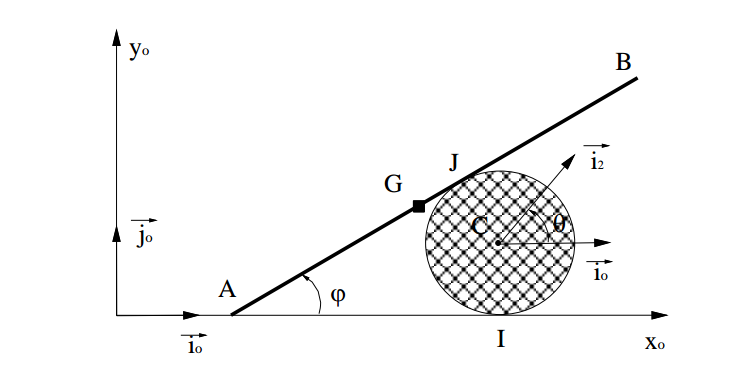
\includegraphics[width=0.85\textwidth]{images/im103.png}
\end{center}

La résolution complète conduit aux schémas suivants :

\begin{center}
  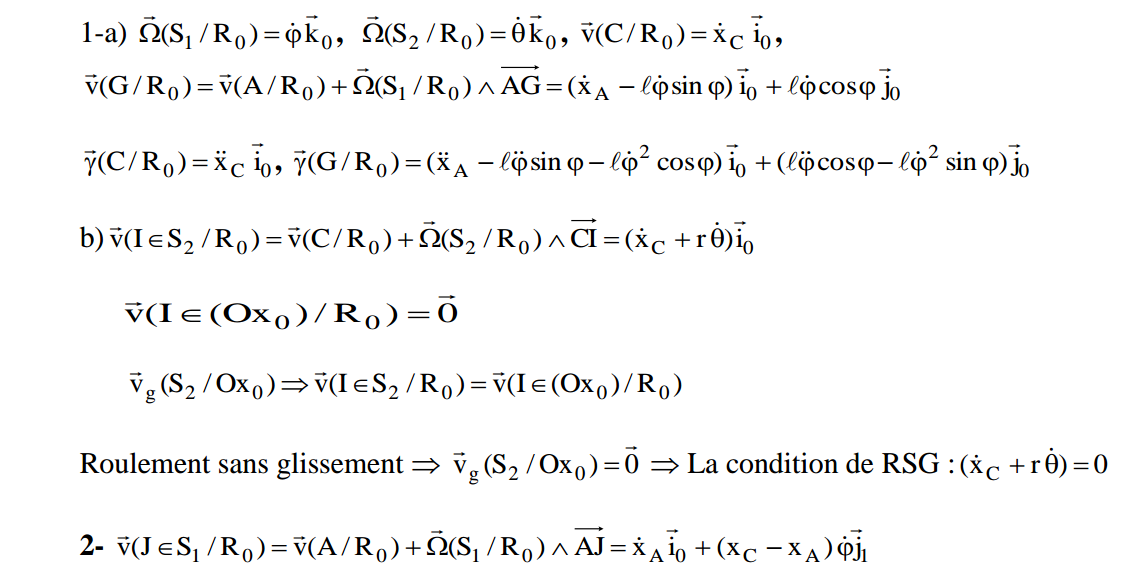
\includegraphics[width=0.85\textwidth]{images/im104.png}
\end{center}
\begin{center}
  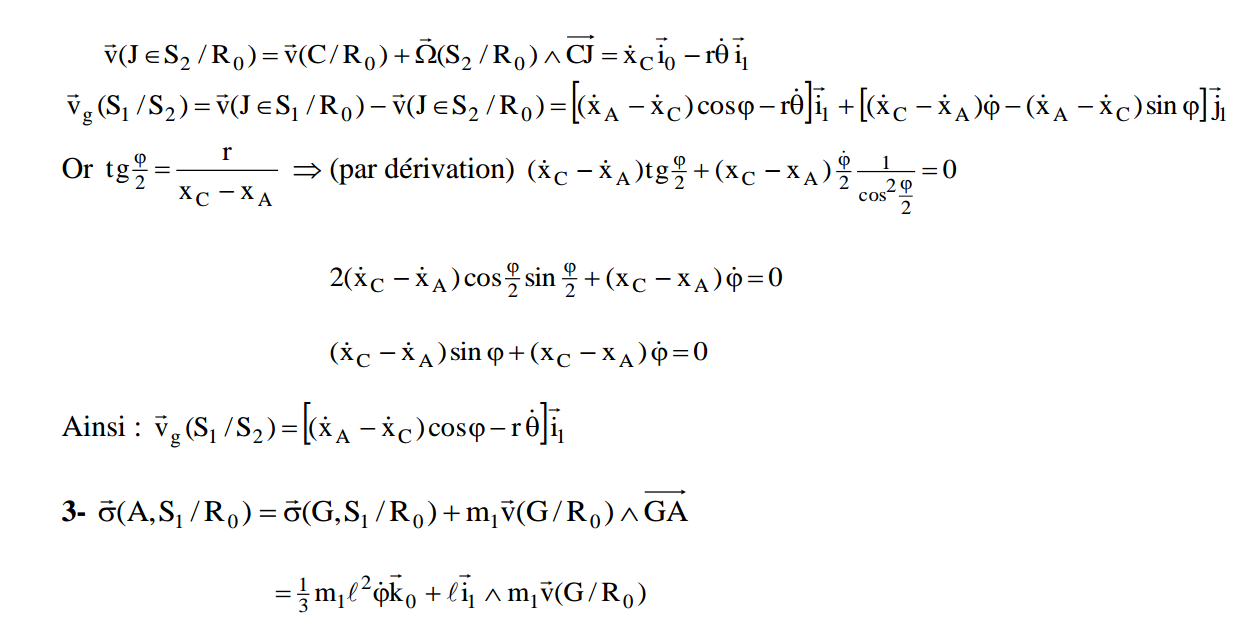
\includegraphics[width=0.85\textwidth]{images/im106.png}
\end{center}
\begin{center}
  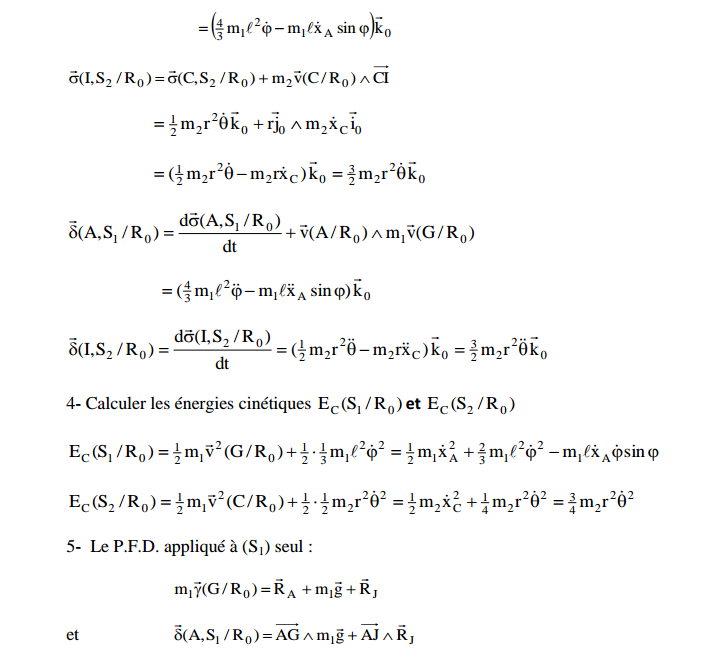
\includegraphics[width=0.85\textwidth]{images/im107.png}
\end{center}

\textbf{Éléments clés de la résolution :}

\textbf{1. Cinématique.}
\[
\vec{\Omega}(S_1/R_0) = \dot\varphi\,\vec{k}_0, \qquad
\vec{\Omega}(S_2/R_0) = \dot\theta\,\vec{k}_0.
\]
\[
\vec{v}(G/R_0) = \dot x_A\,\vec{i}_0 + \ell\dot\varphi\,\vec{j}_1.
\]

Condition de roulement sans glissement de $(S_2)$ sur $Ox_0$ :
\[
\vec{v}(I\in S_2/R_0) = \vec{0} \implies \dot x_C = r\dot\theta.
\]

\textbf{2. Application du P.F.D.}
En appliquant le P.F.D.\ à $(S_1)$ seul (théorème du centre de masse + moment en $A$) et à $(S_2)$ seul (théorème du centre de masse + moment en $C$), on obtient 6 équations scalaires pour les 8 inconnues
\[
(x_A,\, x_C,\, \varphi,\, \theta,\, R_A,\, T_J,\, T_I,\, N_I).
\]
Les liaisons géométriques de contact fournissent les 2 équations manquantes.
\end{boitecorrige}

\ifdefined\inMainDoc\else\end{document}\fi


% ================================================================
%  UE 7 : PROBABILITÉS ET STATISTIQUES
% ================================================================
\newpage
\thispagestyle{empty}
\begin{tikzpicture}[remember picture, overlay]
  \fill[gray!12] ([xshift=1.5cm, yshift=3cm]current page.south west)
    rectangle ([xshift=-1.5cm, yshift=-3cm]current page.north east);
  \draw[line width=3pt] ([xshift=1.5cm,yshift=-3cm]current page.north west)
    -- ([xshift=-1.5cm,yshift=-3cm]current page.north east);
  \draw[line width=3pt] ([xshift=1.5cm,yshift=3cm]current page.south west)
    -- ([xshift=-1.5cm,yshift=3cm]current page.south east);
  \node[align=center] at (current page.center) {%
    {\fontsize{28}{36}\bfseries\selectfont PROBABILITÉS ET STATISTIQUES}\\[1.2cm]
    {\large\itshape Variables aléatoires - Lois usuelles}\\[0.4cm]
    {\large\itshape Estimation et tests statistiques}\\[1.8cm]
    {\normalsize Licence 2 - UE 7}
  };
  \node[anchor=south west] at ([xshift=2cm,yshift=2cm]current page.south west)
    {\large\bfseries UE 7};
\end{tikzpicture}
\newpage

\addcontentsline{toc}{section}{PROBABILITÉS ET STATISTIQUES}
\ifdefined\inMainDoc\else
\documentclass[12pt,a4paper]{article}
% ================================================================
%  PRÉAMBULE COMMUN - ANNALES CORRIGÉES
%  Université de Kara - FaST - Licence Fondamentale MPC
%  Design optimisé impression noir et blanc
% ================================================================

% -- ENCODAGE & LANGUE --
\usepackage[utf8]{inputenc}
\usepackage[T1]{fontenc}
\usepackage[french]{babel}
\usepackage{lmodern}
\usepackage{microtype}

% -- MISE EN PAGE --
\usepackage[a4paper, top=2.8cm, bottom=2.5cm, left=2.5cm, right=2.5cm, headheight=14pt]{geometry}
\usepackage{setspace}
\setstretch{1.2}
\usepackage{parskip}
\setlength{\parindent}{1.2em}
\setlength{\parskip}{4pt}

% -- MATHS --
\usepackage{amsmath, amssymb, mathtools, amsthm}
\usepackage{mathrsfs}
\usepackage{dsfont}
\usepackage{bm}
\usepackage{cancel}
\usepackage{textcomp}
% Définition de \oiint (intégrale de surface fermée) sans package supplémentaire
\newcommand{\oiint}{\mathop{\iint\!\!\!\!\!\!\!\bigcirc}\limits}

% -- PHYSIQUE & CHIMIE --
\usepackage{physics}
\usepackage{siunitx}
% Lorsque physics est chargé, siunitx omet \qty. On le restaure ici :
\AtBeginDocument{\RenewCommandCopy\qty\SI}
\sisetup{locale = FR, detect-all, output-decimal-marker={,}}
% Commande de substitution pour les unités posant problème avec pdflatex
% (ohm, degreeCelsius, micro, angstrom, percent utilisent des caractères non-ASCII)
\newcommand{\qtyohm}[1]{\ensuremath{\num{#1}\,\Omega}}
\newcommand{\qtydegc}[1]{\ensuremath{\num{#1}\,{}^\circ\text{C}}}
\newcommand{\qtyangstrom}[1]{\ensuremath{\num{#1}\,\text{\AA}}}
\newcommand{\qtypercent}[1]{\ensuremath{\num{#1}\,\%}}
\newcommand{\qtyum}[1]{\ensuremath{\num{#1}\,\mu\text{m}}}
\usepackage[version=4]{mhchem}

% -- GRAPHISMES --
\usepackage{graphicx}
\usepackage{float}
\usepackage{caption}
\usepackage{subcaption}
\usepackage{wrapfig}
\usepackage{tikz}
\usetikzlibrary{calc, arrows.meta, patterns, shapes.geometric}
\usepackage{pgfplots}
\pgfplotsset{compat=1.18}

% -- TABLEAUX --
\usepackage{booktabs}
\usepackage{array}
\usepackage{tabularx}
\usepackage{multirow}

% -- LISTES --
\usepackage{enumitem}
\setlist[enumerate]{topsep=3pt, itemsep=2pt, parsep=0pt}
\setlist[itemize]{topsep=3pt, itemsep=2pt, parsep=0pt, label={.}}

% -- BOÎTES (noir et blanc) --
\usepackage{mdframed}
\usepackage{tcolorbox}
\tcbuselibrary{skins, breakable, theorems}

% Boîte EXERCICE : encadré avec filet épais, fond blanc
\newmdenv[
  linewidth=1.2pt,
  linecolor=black,
  roundcorner=3pt,
  skipabove=10pt,
  skipbelow=6pt,
  innertopmargin=8pt,
  innerbottommargin=8pt,
  innerleftmargin=10pt,
  innerrightmargin=10pt,
  backgroundcolor=white,
  frametitle={\bfseries\small Exercice},
  frametitlealignment=\raggedright,
  frametitleaboveskip=4pt,
  frametitlebelowskip=4pt,
]{boiteexercice}

% Boîte CORRIGÉ : fond gris très clair + filet fin
\newmdenv[
  linewidth=0.6pt,
  linecolor=black,
  leftline=true,
  rightline=false,
  topline=false,
  bottomline=false,
  linecolor=black,
  innerleftmargin=12pt,
  innerrightmargin=8pt,
  innertopmargin=6pt,
  innerbottommargin=6pt,
  backgroundcolor=gray!8,
  skipabove=4pt,
  skipbelow=8pt,
]{boitecorrige}

% Boîte RÉSUMÉ DE COURS : double encadré
\newmdenv[
  linewidth=0.8pt,
  linecolor=black,
  roundcorner=2pt,
  backgroundcolor=gray!12,
  innertopmargin=10pt,
  innerbottommargin=10pt,
  innerleftmargin=12pt,
  innerrightmargin=12pt,
  skipabove=12pt,
  skipbelow=8pt,
]{boiteresume}

% Boîte ATTENTION/REMARQUE : barre gauche épaisse
\newmdenv[
  leftline=true,
  rightline=false,
  topline=false,
  bottomline=false,
  linewidth=3pt,
  linecolor=black,
  backgroundcolor=gray!5,
  innerleftmargin=12pt,
  innerrightmargin=8pt,
  innertopmargin=5pt,
  innerbottommargin=5pt,
  skipabove=6pt,
  skipbelow=6pt,
]{boiteremarque}

% -- DIFFICULTÉ DES EXERCICES --
\newcommand{\facile}{$\star$}
\newcommand{\moyen}{$\star\!\star$}
\newcommand{\difficile}{$\star\!\star\!\star$}
\newcommand{\niveau}[1]{\hfill\textbf{#1}\hspace{2pt}}

% -- EN-TÊTES ET PIEDS DE PAGE --
\usepackage{fancyhdr}
\pagestyle{fancy}
\fancyhf{}
\renewcommand{\headrulewidth}{0.5pt}
\renewcommand{\footrulewidth}{0.3pt}

% -- HYPERLIENS --
\usepackage[hidelinks]{hyperref}
\hypersetup{
    colorlinks=false,
    pdftitle={Annale Corrigée - Licence MPC - Université de Kara}
}

% -- TITRES --
\usepackage{titlesec}
\titleformat{\section}{\Large\bfseries}{\thesection.}{0.8em}{}[\vspace{2pt}\hrule\vspace{4pt}]
\titleformat{\subsection}{\large\bfseries}{\thesubsection.}{0.7em}{}
\titleformat{\subsubsection}{\normalsize\bfseries}{\thesubsubsection.}{0.6em}{}

% -- THÉORÈMES --
\theoremstyle{definition}
\newtheorem{defn}{Définition}[section]
\newtheorem{prop}{Propriété}[section]
\newtheorem{thm}{Théorème}[section]
\newtheorem{corol}{Corollaire}[section]
\newtheorem{exemple}{Exemple}[section]

% -- COMMANDES MATHÉMATIQUES UTILES --
\newcommand{\vect}[1]{\overrightarrow{#1}}
\newcommand{\R}{\mathbb{R}}
\newcommand{\N}{\mathbb{N}}
\newcommand{\Z}{\mathbb{Z}}
\newcommand{\C}{\mathbb{C}}
\renewcommand{\d}{\mathrm{d}}
\newcommand{\deriv}[2]{\dfrac{\d #1}{\d #2}}
\newcommand{\dpart}[2]{\dfrac{\partial #1}{\partial #2}}
\newcommand{\rot}{\overrightarrow{\mathrm{rot}}\,}
\renewcommand{\div}{\mathrm{div}\,}
\renewcommand{\grad}{\overrightarrow{\mathrm{grad}}\,}
\newcommand{\e}{\mathrm{e}}
\newcommand{\ii}{\mathrm{i}}
\renewcommand{\Tr}{\mathrm{Tr}}

% Numérotation des équations par section
\numberwithin{equation}{section}

% -- RÉSULTATS ENCADRÉS --
\newcommand{\res}[1]{\[\boxed{#1}\]}

% -- REMARQUE INLINE --
\newcommand{\rmq}[1]{\begin{boiteremarque}\textbf{Remarque.} #1\end{boiteremarque}}

% -- MISE EN VALEUR DU RÉSULTAT FINAL --
\newcommand{\reponse}[1]{%
  \begin{center}
    \fbox{\begin{minipage}{0.92\textwidth}\centering #1\end{minipage}}
  \end{center}%
}


% En-têtes et pieds de page
\lhead{\textbf{Probabilités et Statistiques} - Licence 2}
\rhead{Université de Kara - FaST}
\cfoot{\thepage}
\lfoot{\textit{Licence Fondamentale MPC}}
\rfoot{\textit{Annales corrigées}}

\begin{document}
\fi

\begin{center}
  {\LARGE\bfseries Probabilités et Statistiques}\\[6pt]
  {\large Licence 2 - Mathématiques, Physique, Chimie}\\[4pt]
  {\normalsize Université de Kara - Faculté des Sciences et Techniques}
\end{center}

\vspace{8pt}
\hrule
\vspace{12pt}

% ================================================================
\section{Résumé de cours}
% ================================================================

\begin{boiteresume}
\textbf{1. Dénombrement}

Soit $n, k \in \mathbb{N}$ avec $k \leq n$.
\begin{itemize}
  \item \textbf{Arrangements} (ordre compte, sans répétition) : $A_n^k = \dfrac{n!}{(n-k)!}$
  \item \textbf{Permutations} de $n$ éléments : $P_n = n!$
  \item \textbf{Combinaisons} (ordre ne compte pas) : $\dbinom{n}{k} = \dfrac{n!}{k!\,(n-k)!}$
  \item \textbf{Formule de Pascal} : $\dbinom{n}{k} + \dbinom{n}{k+1} = \dbinom{n+1}{k+1}$
\end{itemize}

\medskip
\textbf{2. Probabilités - Axiomes de Kolmogorov}

Un espace de probabilité $(\Omega, \mathcal{A}, P)$ vérifie :
\begin{itemize}
  \item $P(\Omega) = 1$ et $P(A) \geq 0$ pour tout événement $A$.
  \item Additivité : si $A \cap B = \emptyset$ alors $P(A \cup B) = P(A) + P(B)$.
  \item $P(\bar{A}) = 1 - P(A)$.
\end{itemize}

\textbf{Probabilité conditionnelle} : $P(A \mid B) = \dfrac{P(A \cap B)}{P(B)}$ pour $P(B) > 0$.

\textbf{Formule des probabilités totales} : si $(A_i)$ est une partition de $\Omega$,
\[
P(B) = \sum_{i} P(B \mid A_i)\,P(A_i).
\]

\textbf{Théorème de Bayes} :
\[
P(A_i \mid B) = \frac{P(B \mid A_i)\,P(A_i)}{\displaystyle\sum_{j} P(B \mid A_j)\,P(A_j)}.
\]

\textbf{Indépendance} : $A$ et $B$ sont indépendants si et seulement si $P(A \cap B) = P(A)\,P(B)$.

\medskip
\textbf{3. Variables aléatoires discrètes}

Pour $X$ à valeurs dans $\{x_1, x_2, \ldots\}$ :
\[
\mathbb{E}(X) = \sum_i x_i\,P(X=x_i), \qquad
V(X) = \mathbb{E}(X^2) - [\mathbb{E}(X)]^2, \qquad
\sigma(X) = \sqrt{V(X)}.
\]

\begin{itemize}
  \item \textbf{Loi binomiale} $\mathcal{B}(n,p)$ : $P(X=k) = \dbinom{n}{k} p^k (1-p)^{n-k}$, $\mathbb{E}(X)=np$, $V(X)=np(1-p)$.
  \item \textbf{Loi de Poisson} $\mathcal{P}(\lambda)$ : $P(X=k) = \dfrac{\lambda^k}{k!}\,\mathrm{e}^{-\lambda}$, $\mathbb{E}(X)=\lambda$, $V(X)=\lambda$.
\end{itemize}

\medskip
\textbf{4. Variables aléatoires continues}

Densité $f \geq 0$ avec $\displaystyle\int_{-\infty}^{+\infty} f(x)\,\d x = 1$.
\[
\mathbb{E}(X) = \int x\,f(x)\,\mathrm{d}x, \qquad
V(X) = \int x^2 f(x)\,\mathrm{d}x - [\mathbb{E}(X)]^2.
\]

\begin{itemize}
  \item \textbf{Loi uniforme} $\mathcal{U}([a,b])$ : $f(x)=\dfrac{1}{b-a}$ sur $[a,b]$, $\mathbb{E}(X)=\dfrac{a+b}{2}$, $V(X)=\dfrac{(b-a)^2}{12}$.
  \item \textbf{Loi exponentielle} $\mathcal{E}(\lambda)$ : $f(x)=\lambda\,\mathrm{e}^{-\lambda x}$ pour $x\geq 0$, $\mathbb{E}(X)=\dfrac{1}{\lambda}$, $V(X)=\dfrac{1}{\lambda^2}$.
  \item \textbf{Loi normale} $\mathcal{N}(m,\sigma^2)$ : $f(x)=\dfrac{1}{\sigma\sqrt{2\pi}}\,\mathrm{e}^{-\frac{(x-m)^2}{2\sigma^2}}$, $\mathbb{E}(X)=m$, $V(X)=\sigma^2$.
\end{itemize}

\medskip
\textbf{5. Statistiques descriptives}

Pour une série de valeurs $x_1, \ldots, x_n$ :
\[
\bar{x} = \frac{1}{n}\sum x_i, \quad
s^2 = \frac{1}{n}\sum x_i^2 - \bar{x}^2, \quad
s = \sqrt{s^2}.
\]
La \textbf{médiane} $M_e$ vérifie $F(M_e) = 0{,}5$. Le \textbf{mode} est la valeur (ou classe) de plus grande fréquence. Les \textbf{quartiles} $Q_1$, $Q_2$, $Q_3$ correspondent aux fréquences cumulées $0{,}25$, $0{,}5$, $0{,}75$.
\end{boiteresume}

% ================================================================
\section{Exercices corrigés}
% ================================================================

% ----------------------
\begin{boiteexercice}
\textbf{Exercice 1 - Dénombrement dans un jeu de cartes}\niveau{\facile}

On tire simultanément 5 cartes d'un jeu de 32 cartes. Combien de tirages différents peut-on obtenir :
\begin{enumerate}
  \item sans contrainte sur les cartes ;
  \item contenant 5 carreaux ou 5 piques ;
  \item contenant 2 carreaux et 3 piques ;
  \item contenant au moins un roi ;
  \item contenant au plus un roi ;
  \item contenant exactement 2 rois et exactement 3 piques.
\end{enumerate}
\end{boiteexercice}

\begin{boitecorrige}
\textbf{1.} Un tirage est une combinaison de 5 cartes parmi 32 :
\[
\binom{32}{5} = 201\,376 \text{ tirages.}
\]

\textbf{2.} Choisir 5 carreaux parmi 8 ou 5 piques parmi 8 (cas disjoints) :
\[
2 \times \binom{8}{5} = 2 \times 56 = 112 \text{ tirages.}
\]

\textbf{3.} Choisir 2 carreaux parmi 8 puis 3 piques parmi 8 :
\[
\binom{8}{2} \times \binom{8}{3} = 28 \times 56 = 1\,568 \text{ tirages.}
\]

\textbf{4.} Par complémentaire (aucun roi : choisir 5 cartes parmi les 28 non-rois) :
\[
\binom{32}{5} - \binom{28}{5} = 201\,376 - 98\,280 = 103\,096 \text{ tirages.}
\]

\textbf{5.} Tirages sans roi : $\binom{28}{5}$. Tirages avec exactement un roi : $4 \times \binom{28}{4}$.
\[
\binom{28}{5} + 4\binom{28}{4} = 98\,280 + 4 \times 20\,475 = 180\,180 \text{ tirages.}
\]

\textbf{6.} On distingue deux cas selon que le roi de pique est présent ou non.

Si le tirage ne contient pas le roi de pique : choisir 2 rois parmi les 3 autres, puis 3 piques parmi les 7 piques non-rois.
\[
\binom{3}{2} \times \binom{7}{3} = 3 \times 35 = 105 \text{ tirages.}
\]

Si le tirage contient le roi de pique : choisir 1 roi parmi les 3 autres, 2 piques non-rois parmi 7, puis 1 carte ni roi ni pique parmi $32 - 4 - 7 = 21$.
\[
3 \times \binom{7}{2} \times 21 = 3 \times 21 \times 21 = 1\,323 \text{ tirages.}
\]

Total : $105 + 1\,323 = 1\,428$ tirages.
\end{boitecorrige}

% ----------------------
\begin{boiteexercice}
\textbf{Exercice 2 - Probabilités conditionnelles et théorème de Bayes}\niveau{\moyen}

Une urne $U_1$ contient 4 jetons blancs et 3 noirs ; une urne $U_2$ contient 17 jetons blancs et 18 noirs.

\textbf{Partie 1.} On lance un dé cubique équilibré. Si 6 apparaît, on tire de $U_1$, sinon de $U_2$. On note $A$ : « on a obtenu 6 » et $B$ : « on tire un jeton blanc ».
\begin{itemize}
  \item[a.] Calculer $P(B)$.
  \item[b.] Sachant qu'on a tiré un jeton blanc, calculer $P(A \mid B)$.
  \item[c.] Sachant qu'on a tiré un jeton noir, calculer $P(\bar{A} \mid \bar{B})$.
\end{itemize}

\textbf{Partie 2.} On tire successivement et sans remise les 7 jetons de $U_1$. La variable $X$ prend la valeur $k$ si le premier jeton blanc apparaît au $k$-ième tirage. Donner la loi de $X$, puis calculer son espérance et son écart-type.
\end{boiteexercice}

\begin{boitecorrige}
\textbf{Partie 1.}

On a $P(A) = \tfrac{1}{6}$, $P(\bar{A}) = \tfrac{5}{6}$, $P(B \mid A) = \tfrac{4}{7}$, $P(B \mid \bar{A}) = \tfrac{17}{35}$.

\textbf{a.} Par la formule des probabilités totales :
\[
P(B) = P(B \mid A)\,P(A) + P(B \mid \bar{A})\,P(\bar{A})
= \frac{4}{7} \cdot \frac{1}{6} + \frac{17}{35} \cdot \frac{5}{6}
= \frac{4}{42} + \frac{85}{210} = \frac{20}{210} + \frac{85}{210} = \frac{1}{2}.
\]

\textbf{b.} Par Bayes :
\[
P(A \mid B) = \frac{P(B \mid A)\,P(A)}{P(B)} = \frac{\tfrac{4}{7} \times \tfrac{1}{6}}{\tfrac{1}{2}} = \frac{4}{21}.
\]

\textbf{c.} $P(\bar{B}) = 1 - P(B) = \tfrac{1}{2}$. $P(\bar{B} \mid \bar{A}) = \tfrac{18}{35}$.
\[
P(\bar{A} \mid \bar{B}) = \frac{P(\bar{B} \mid \bar{A})\,P(\bar{A})}{P(\bar{B})} = \frac{\tfrac{18}{35} \times \tfrac{5}{6}}{\tfrac{1}{2}} = \frac{6}{7}.
\]

\textbf{Partie 2.} $U_1$ contient 4 blancs et 3 noirs, 7 jetons en tout. $X$ prend ses valeurs dans $\{1, 2, 3, 4\}$.

\[
\begin{array}{|c|c|c|c|c|}
\hline
k & 1 & 2 & 3 & 4 \\
\hline
P(X=k) & \dfrac{4}{7} & \dfrac{2}{7} & \dfrac{4}{35} & \dfrac{1}{35} \\
\hline
\end{array}
\]

Vérification : $\tfrac{4}{7} + \tfrac{2}{7} + \tfrac{4}{35} + \tfrac{1}{35} = \tfrac{20+10+4+1}{35} = 1$.

\[
\mathbb{E}(X) = 1 \cdot \frac{4}{7} + 2 \cdot \frac{2}{7} + 3 \cdot \frac{4}{35} + 4 \cdot \frac{1}{35}
= \frac{20 + 20 + 12 + 4}{35} = \frac{56}{35} = \frac{8}{5}.
\]

\[
\mathbb{E}(X^2) = 1 \cdot \frac{4}{7} + 4 \cdot \frac{2}{7} + 9 \cdot \frac{4}{35} + 16 \cdot \frac{1}{35}
= \frac{20 + 40 + 36 + 16}{35} = \frac{112}{35} = \frac{16}{5}.
\]

\[
V(X) = \frac{16}{5} - \left(\frac{8}{5}\right)^2 = \frac{16}{5} - \frac{64}{25} = \frac{80 - 64}{25} = \frac{16}{25}.
\qquad \sigma(X) = \frac{4}{5} = 0{,}8.
\]
\end{boitecorrige}

% ----------------------
\begin{boiteexercice}
\textbf{Exercice 3 - Variables aléatoires discrètes, covariance}\niveau{\moyen}

Soit $X$ une variable aléatoire dont la loi est donnée par :
\[
\begin{array}{|c|c|c|c|c|c|}
\hline
k & -2 & -1 & 0 & 1 & 2 \\
\hline
P(X=k) & \dfrac{1}{6} & \dfrac{1}{4} & \dfrac{1}{6} & \dfrac{1}{4} & \dfrac{1}{6} \\
\hline
\end{array}
\]
On pose $Y = X^2$.
\begin{enumerate}
  \item Déterminer la loi de $Y$.
  \item $X$ et $Y$ sont-elles indépendantes ?
  \item Calculer $\mathrm{Cov}(X, Y)$. Que remarque-t-on ?
\end{enumerate}
\end{boiteexercice}

\begin{boitecorrige}
\textbf{1. Loi de $Y = X^2$.}

$Y$ prend les valeurs $0, 1, 4$.
\[
P(Y=0) = P(X=0) = \frac{1}{6}.
\]
\[
P(Y=1) = P(X=-1) + P(X=1) = \frac{1}{4} + \frac{1}{4} = \frac{1}{2}.
\]
\[
P(Y=4) = P(X=-2) + P(X=2) = \frac{1}{6} + \frac{1}{6} = \frac{1}{3}.
\]

\[
\begin{array}{|c|c|c|c|}
\hline
y & 0 & 1 & 4 \\
\hline
P(Y=y) & \dfrac{1}{6} & \dfrac{1}{2} & \dfrac{1}{3} \\
\hline
\end{array}
\]

\textbf{2. Indépendance.}

Si $X$ et $Y$ étaient indépendantes, on aurait $P(X=-1,\,Y=4) = P(X=-1)\cdot P(Y=4)$. Or $P(X=-1,\,Y=4) = 0$ (car $(-1)^2 = 1 \neq 4$), mais $P(X=-1)\cdot P(Y=4) = \tfrac{1}{4} \times \tfrac{1}{3} = \tfrac{1}{12} \neq 0$. Donc $X$ et $Y$ ne sont pas indépendantes.

\textbf{3. Covariance.}

\[
\mathbb{E}[X] = (-2)\cdot\frac{1}{6} + (-1)\cdot\frac{1}{4} + 0 + 1\cdot\frac{1}{4} + 2\cdot\frac{1}{6} = 0 \quad \text{(loi symétrique).}
\]
\[
\mathbb{E}[Y] = 0 \cdot \frac{1}{6} + 1 \cdot \frac{1}{2} + 4 \cdot \frac{1}{3} = \frac{1}{2} + \frac{4}{3} = \frac{11}{6}.
\]
\[
\mathbb{E}[XY] = \mathbb{E}[X^3] = (-2)^3 \cdot \frac{1}{6} + (-1)^3 \cdot \frac{1}{4} + 0 + 1^3 \cdot \frac{1}{4} + 2^3 \cdot \frac{1}{6} = 0.
\]
\[
\mathrm{Cov}(X,Y) = \mathbb{E}[XY] - \mathbb{E}[X]\,\mathbb{E}[Y] = 0 - 0 = 0.
\]

Remarque : la covariance nulle ne suffit pas à établir l'indépendance. Ici, $X$ et $Y$ sont non corrélées mais non indépendantes.
\end{boitecorrige}

% ----------------------
\begin{boiteexercice}
\textbf{Exercice 4 - Loi de Poisson et couple de variables aléatoires}\niveau{\difficile}

Soient $X$ et $Y$ des variables aléatoires à valeurs dans $\mathbb{N}$ telles que, pour tout $(i,j) \in \mathbb{N}^2$ :
\[
P\bigl([X=i] \cap [Y=j]\bigr) = \frac{\alpha}{2^{i+j}\,j!}.
\]
\begin{enumerate}
  \item Déterminer $\alpha$.
  \item Déterminer les lois marginales de $X$ et de $Y$.
  \item Calculer $\mathrm{Cov}(X,Y)$. $X$ et $Y$ sont-elles indépendantes ?
\end{enumerate}
\end{boiteexercice}

\begin{boitecorrige}
\textbf{1. Détermination de $\alpha$.}

La somme de toutes les probabilités doit être égale à 1 :
\[
\sum_{i=0}^{\infty}\sum_{j=0}^{\infty} \frac{\alpha}{2^{i+j}\,j!}
= \alpha \left(\sum_{i=0}^{\infty} \frac{1}{2^i}\right)\left(\sum_{j=0}^{\infty} \frac{1}{2^j\,j!}\right)
= \alpha \cdot \frac{1}{1-\tfrac{1}{2}} \cdot \mathrm{e}^{1/2}
= 2\alpha\,\mathrm{e}^{1/2} = 1.
\]
Donc $\alpha = \dfrac{1}{2\,\mathrm{e}^{1/2}} = \dfrac{\mathrm{e}^{-1/2}}{2}$.

\textbf{2. Lois marginales.}

Loi de $X$ :
\[
P(X=i) = \sum_{j=0}^{\infty} \frac{\alpha}{2^{i+j}\,j!}
= \frac{\alpha}{2^i}\,\mathrm{e}^{1/2} = \frac{\mathrm{e}^{-1/2}}{2} \cdot \frac{\mathrm{e}^{1/2}}{2^i} = \frac{1}{2^{i+1}}.
\]
C'est une loi géométrique sur $\mathbb{N}$ de paramètre $\tfrac{1}{2}$ (avec $i \geq 0$).

Loi de $Y$ :
\[
P(Y=j) = \sum_{i=0}^{\infty} \frac{\alpha}{2^{i+j}\,j!}
= \frac{\alpha}{2^j\,j!} \cdot 2 = \frac{\mathrm{e}^{-1/2}}{2^j\,j!}.
\]
En posant $\lambda = \tfrac{1}{2}$, on reconnaît $P(Y=j) = \dfrac{\mathrm{e}^{-\lambda}\,\lambda^j}{j!}$ : c'est une loi de Poisson $\mathcal{P}\!\left(\tfrac{1}{2}\right)$.

\textbf{3. Covariance.}

$\mathbb{E}(X) = \displaystyle\sum_{i=0}^{\infty} \frac{i}{2^{i+1}} = \frac{1}{2}\cdot\frac{1/(1-1/2)^2}{2} = 1$ (série arithmético-géométrique).

$\mathbb{E}(Y) = \lambda = \tfrac{1}{2}$ (espérance de $\mathcal{P}(\tfrac{1}{2})$).

\[
\mathbb{E}(XY) = \sum_{i,j} ij \cdot \frac{\alpha}{2^{i+j}\,j!}
= \alpha \left(\sum_i \frac{i}{2^i}\right)\!\left(\sum_j \frac{j}{2^j\,j!}\right)
= \alpha \cdot 2 \cdot \frac{\mathrm{e}^{1/2}}{4} = \frac{1}{2}.
\]

\[
\mathrm{Cov}(X,Y) = \mathbb{E}(XY) - \mathbb{E}(X)\,\mathbb{E}(Y) = \frac{1}{2} - 1 \cdot \frac{1}{2} = 0.
\]

De plus, $P(X=i)\cdot P(Y=j) = \dfrac{1}{2^{i+1}} \cdot \dfrac{\mathrm{e}^{-1/2}}{2^j\,j!} = \dfrac{\mathrm{e}^{-1/2}}{2^{i+j+1}\,j!} = P(X=i,\,Y=j)$.

Donc $X$ et $Y$ sont indépendantes (et la covariance nulle en est la conséquence).
\end{boitecorrige}

% ----------------------
\begin{boiteexercice}
\textbf{Exercice 5 - Statistiques descriptives : loyers}\niveau{\moyen}

Une enquête sur les loyers annuels (en milliers de francs) d'un quartier donne :

\[
\begin{array}{|c|c|}
\hline
\text{Classe de loyer} & \text{Effectif} \\
\hline
{[4\,;\,6[} & 20 \\
{[6\,;\,8[} & 40 \\
{[8\,;\,10[} & 80 \\
{[10\,;\,15[} & 30 \\
{[15\,;\,20[} & 20 \\
{[20\,;\,30[} & 10 \\
\hline
\end{array}
\]

\begin{enumerate}
  \item Compléter le tableau (valeur centrale, fréquence, fréquences cumulées, densité).
  \item Déterminer la moyenne, le mode et les quartiles $Q_1$, $Q_2$, $Q_3$.
  \item Calculer l'étendue, l'écart-type et l'intervalle interquartile.
\end{enumerate}
\end{boiteexercice}

\begin{boitecorrige}
L'effectif total est $n = 200$.

\textbf{1. Tableau complété.}

\[
\begin{array}{|c|c|c|c|c|c|}
\hline
\text{Classe} & x_i & n_i & N_i & f_i & d_i \\
\hline
{[4;6[}   & 5  & 20  & 20  & 0{,}10 & 10 \\
{[6;8[}   & 7  & 40  & 60  & 0{,}20 & 20 \\
{[8;10[}  & 9  & 80  & 140 & 0{,}40 & 40 \\
{[10;15[} & 12{,}5 & 30 & 170 & 0{,}15 & 6 \\
{[15;20[} & 17{,}5 & 20 & 190 & 0{,}10 & 4 \\
{[20;30[} & 25 & 10  & 200 & 0{,}05 & 1 \\
\hline
\end{array}
\]

\textbf{2. Moyenne, mode, quartiles.}

\[
\bar{x} = \sum f_i\,x_i = 0{,}10\times5 + 0{,}20\times7 + 0{,}40\times9 + 0{,}15\times12{,}5 + 0{,}10\times17{,}5 + 0{,}05\times25 = 10{,}375.
\]

La classe modale est $[8\,;\,10[$ (densité maximale $= 40$).
\[
M_o = 8 + \frac{40-20}{(40-20)+(40-30)} \times 2 = 8 + \frac{20}{30} \times 2 \approx 9{,}33.
\]

Pour les quartiles, on utilise $Q_p = a_i + (a_{i+1}-a_i)\cdot\dfrac{p\,n/4 - N_{i-1}}{n_i}$ :
\[
Q_1 : F = 0{,}25,\text{ classe } [8;10[. \quad Q_1 = 8 + 2 \cdot \frac{0{,}25 - 0{,}30}{0{,}40} = 7{,}5 \times 10^3.
\]
\[
Q_2 : F = 0{,}50,\text{ classe } [8;10[. \quad Q_2 = 8 + 2 \cdot \frac{0{,}50 - 0{,}30}{0{,}40} = 9{,}0 \times 10^3.
\]
\[
Q_3 : F = 0{,}75,\text{ classe } [10;15[. \quad Q_3 = 10 + 5 \cdot \frac{0{,}75 - 0{,}70}{0{,}15} \approx 11{,}67 \times 10^3.
\]

\textbf{3. Dispersion.}

Étendue : $W = (30-4) \times 1000 = 26\,000$ F.

Intervalle interquartile : $\mathrm{IQ} = Q_3 - Q_1 = (11\,667 - 7\,500) = 4\,167$ F.

\[
\sigma^2 = \sum f_i\,x_i^2 - \bar{x}^2, \qquad \sigma \approx 5{,}43 \times 10^3 \text{ F}.
\]
\end{boitecorrige}

% ----------------------
\begin{boiteexercice}
\textbf{Exercice 6 - Régression linéaire}\niveau{\moyen}

On dispose des données suivantes (5 points) :
\[
\begin{array}{c|ccccc}
x_i & 2 & 5 & 6 & 10 & 12 \\
\hline
y_i & 83 & 70 & 70 & 54 & 49
\end{array}
\]
\begin{enumerate}
  \item Calculer la covariance $\mathrm{Cov}(X,Y)$.
  \item Déterminer l'équation de la droite de régression $Y = aX + b$.
  \item Calculer le coefficient de corrélation linéaire $r$ et commenter.
\end{enumerate}
\end{boiteexercice}

\begin{boitecorrige}
$n = 5$.

\[
\bar{X} = \frac{2+5+6+10+12}{5} = 7, \qquad \bar{Y} = \frac{83+70+70+54+49}{5} = 65{,}2.
\]

\textbf{1.}
\[
\mathrm{Cov}(X,Y) = \frac{1}{n}\sum X_i Y_i - \bar{X}\,\bar{Y}
= \frac{\sum X_i Y_i}{5} - 7 \times 65{,}2.
\]
où $\sum X_i Y_i = 2\cdot83 + 5\cdot70 + 6\cdot70 + 10\cdot54 + 12\cdot49$.
\[
\frac{166 + 350 + 420 + 540 + 588}{5} = \frac{2064}{5} = 412{,}8.
\quad \mathrm{Cov}(X,Y) = 412{,}8 - 456{,}4 = -43{,}6.
\]

\textbf{2.}
\[
V(X) = \frac{1}{n}\sum X_i^2 - \bar{X}^2 = \frac{4+25+36+100+144}{5} - 49 = 61{,}8 - 49 = 12{,}8.
\]
\[
a = \frac{\mathrm{Cov}(X,Y)}{V(X)} = \frac{-43{,}6}{12{,}8} \approx -3{,}406, \qquad
b = \bar{Y} - a\bar{X} = 65{,}2 - (-3{,}406)\times 7 \approx 89.
\]
\[
\boxed{Y = -3{,}41\,X + 89.}
\]

\textbf{3.}
\[
V(Y) = \frac{83^2+70^2+70^2+54^2+49^2}{5} - 65{,}2^2 = 4\,257{,}2 - 4\,251{,}04 \approx 143{,}36.
\]
\[
r = \frac{\mathrm{Cov}(X,Y)}{\sqrt{V(X)\,V(Y)}} = \frac{-43{,}6}{\sqrt{12{,}8 \times 143{,}36}} \approx \frac{-43{,}6}{42{,}83} \approx -1{,}02 \approx -1.
\]

La valeur $r \approx -1$ indique une forte corrélation linéaire négative entre $X$ et $Y$ : quand le chiffre augmente, l'autre diminue de façon quasi proportionnelle.
\end{boitecorrige}

% ----------------------
\begin{boiteexercice}
\textbf{Exercice 7 - Loi normale}\niveau{\moyen}

Montrer que si $X \sim \mathcal{N}(0,1)$, alors $Z = \sigma X + m$ suit une loi $\mathcal{N}(m, \sigma^2)$.

Calculer ensuite $\mathbb{E}(Z)$ et $V(Z)$ directement à partir des propriétés de l'espérance et de la variance.
\end{boiteexercice}

\begin{boitecorrige}
\textbf{Calcul par transformation de la densité.}

La densité de $X \sim \mathcal{N}(0,1)$ est $f_X(x) = \dfrac{1}{\sqrt{2\pi}}\,\mathrm{e}^{-x^2/2}$.

On pose $Z = \sigma X + m$, donc $X = \dfrac{Z-m}{\sigma}$ et $\dfrac{\mathrm{d}x}{\mathrm{d}z} = \dfrac{1}{\sigma}$.

Par la formule de changement de variable :
\[
f_Z(z) = f_X\!\left(\frac{z-m}{\sigma}\right) \cdot \frac{1}{|\sigma|}
= \frac{1}{\sqrt{2\pi}}\,\mathrm{e}^{-\frac{(z-m)^2}{2\sigma^2}} \cdot \frac{1}{\sigma}
= \frac{1}{\sigma\sqrt{2\pi}}\,\mathrm{e}^{-\frac{(z-m)^2}{2\sigma^2}}.
\]

C'est bien la densité d'une loi $\mathcal{N}(m, \sigma^2)$.

\textbf{Par les propriétés de l'espérance et de la variance :}
\[
\mathbb{E}(Z) = \mathbb{E}(\sigma X + m) = \sigma\,\mathbb{E}(X) + m = \sigma \times 0 + m = m.
\]
\[
V(Z) = V(\sigma X + m) = \sigma^2\,V(X) = \sigma^2 \times 1 = \sigma^2.
\]

Ainsi $Z \sim \mathcal{N}(m, \sigma^2)$, ce qui confirme le résultat précédent.
\end{boitecorrige}

\section{Variables aléatoires discrètes et continues}

\subsection*{Exercice 8 - Variable aléatoire uniforme discrète \niveau{\facile}}

\begin{boiteexercice}
Soit $X$ une variable aléatoire de loi uniforme sur $X(\Omega) = \{-3; -2; 1; 4\}$.
\begin{enumerate}
  \item Donner la loi de $X$.
  \item Calculer $\mathbb{E}(X)$ et $V(X)$.
  \item On pose $Y = 2X+1$. Donner $Y(\Omega)$ et la loi de $Y$.
  \item Calculer $\mathbb{E}(Y)$ de deux façons différentes.
\end{enumerate}
\end{boiteexercice}

\begin{boitecorrige}
\textbf{1.} La loi uniforme sur 4 valeurs équiprobables :
\[
P(X=-3)=P(X=-2)=P(X=1)=P(X=4)=\frac{1}{4}
\]

\textbf{2.}
\[
\mathbb{E}(X) = \frac{1}{4}(-3-2+1+4) = \frac{0}{4} = 0
\]
\[
\mathbb{E}(X^2) = \frac{1}{4}(9+4+1+16) = \frac{30}{4} = 7{,}5 \quad\Rightarrow\quad V(X) = 7{,}5 - 0^2 = 7{,}5
\]

\textbf{3.} $Y(\Omega) = \{2(-3)+1, 2(-2)+1, 2(1)+1, 2(4)+1\} = \{-5, -3, 3, 9\}$. Comme $Y$ est une fonction bijective de $X$, chaque valeur a probabilité $1/4$.

\textbf{4.} \emph{Méthode 1 (linéarité de l'espérance)} : $\mathbb{E}(Y) = 2\mathbb{E}(X)+1 = 2\times0+1 = 1$.

\emph{Méthode 2 (calcul direct)} :
\[
\mathbb{E}(Y) = \frac{1}{4}(-5-3+3+9) = \frac{4}{4} = 1
\]
Les deux méthodes donnent $\mathbb{E}(Y) = 1$.
\end{boitecorrige}

\subsection*{Exercice 9 - Statistiques descriptives : loyers \niveau{\moyen}}

\begin{boiteexercice}
Une enquête sur les loyers annuels (en milliers de francs CFA) d'appartements donne :
\[
\begin{array}{|c|c|}
\hline
\text{Classe de loyer (×1000)} & \text{Effectif} \\
\hline
${[}4;6{[}$ & 20 \\
${[}6;8{[}$ & 40 \\
${[}8;10{[}$ & 80 \\
${[}10;15{[}$ & 30 \\
${[}15;20{[}$ & 20 \\
${[}20;30{[}$ & 10 \\
\hline
\end{array}
\]
\begin{enumerate}
  \item Calculer la moyenne, le mode, la médiane et les quartiles $Q_1$, $Q_3$.
  \item Calculer l'étendue, l'écart-type et l'intervalle interquartile.
\end{enumerate}
\end{boiteexercice}

\begin{boitecorrige}
L'effectif total est $n = 200$. Les valeurs centrales des classes sont : $5, 7, 9, 12{,}5, 17{,}5, 25$.

\textbf{1.} Moyenne :
\[
\bar{x} = \frac{1}{200}(20\times5 + 40\times7 + 80\times9 + 30\times12{,}5 + 20\times17{,}5 + 10\times25) = \frac{2075}{200} \approx 10{,}375 \text{ milliers}
\]
La classe modale est $[8;10[$ (plus grande densité $= 80/2 = 40$). Le mode vaut :
\[
M = 8 + \frac{(80-40)}{(80-40)+(80-30)}\times 2 \approx 8{,}89\text{ milliers}
\]
Les effectifs cumulés : $20, 60, 140, 170, 190, 200$. La médiane ($n/2 = 100$) est dans $[8;10[$ :
\[
\text{Médiane} = 8 + \frac{100-60}{80}\times 2 = 8 + 1 = 9\text{ milliers}
\]
$Q_1$ ($n/4=50$) dans $[6;8[$ : $Q_1 = 6 + \frac{50-20}{40}\times2 = 7{,}5$ milliers.

$Q_3$ ($3n/4=150$) dans $[10;15[$ : $Q_3 = 10 + \frac{150-140}{30}\times5 \approx 11{,}67$ milliers.

\textbf{2.} Étendue $= (30-4) = 26$ milliers. Intervalle interquartile $= Q_3-Q_1 \approx 4{,}17$ milliers.

Variance : $\sigma^2 = \frac{1}{200}\sum n_i x_i^2 - \bar{x}^2$. En calculant $\sum n_i x_i^2 = 20(25)+40(49)+80(81)+30(156{,}25)+20(306{,}25)+10(625) = 26\,037{,}5$, d'où $\sigma^2 = 130{,}19 - 107{,}64 \approx 22{,}55$, soit $\sigma \approx 4{,}75$ milliers.

\begin{center}
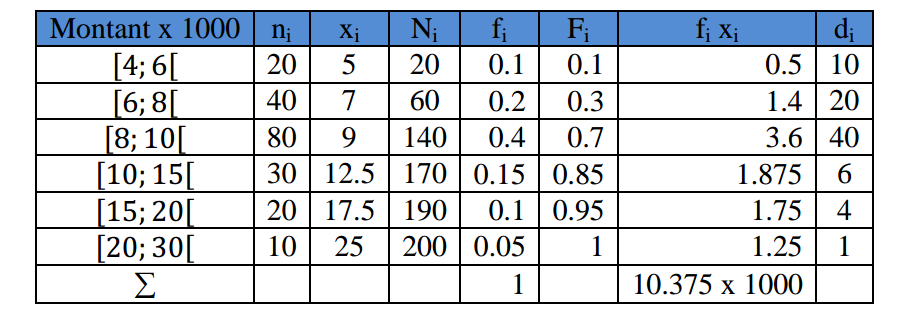
\includegraphics[width=0.85\textwidth]{images/probabilites/prob-015-000.png}\\[4pt]
{\small\itshape Tableau statistique complété (document original).}
\end{center}

\begin{center}

\includegraphics[width=0.85\textwidth]{images/probabilites/prob-015-001.png}\\[4pt]
{\small\itshape Histogramme des effectifs par classe de salaire (document original).}
\end{center}

\begin{center}
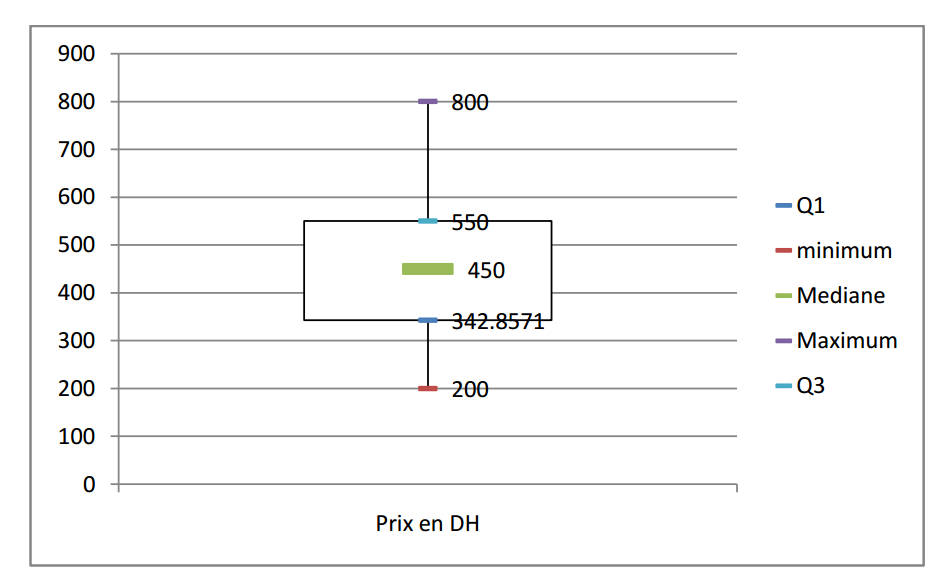
\includegraphics[width=0.6\textwidth]{images/probabilites/prob-017-002.png}\\[4pt]
{\small\itshape Exemple de boîte à moustaches (box-plot) : médiane, quartiles et extrêmes.}
\end{center}

\begin{center}

\includegraphics[width=0.6\textwidth]{images/probabilites/prob-017-003.png}\\[4pt]
{\small\itshape Polygone des fréquences cumulées et médiane graphique.}
\end{center}
\end{boitecorrige}

\subsection*{Exercice 10 - Régression linéaire \niveau{\moyen}}

\begin{boiteexercice}
On dispose de la série double suivante :
\[
\begin{array}{|c|c|c|c|c|c|}
\hline
X_i & 2 & 5 & 6 & 10 & 12 \\
\hline
Y_i & 83 & 70 & 70 & 54 & 49 \\
\hline
\end{array}
\]
\begin{enumerate}
  \item Calculer la covariance $\mathrm{Cov}(X,Y)$.
  \item Déterminer la droite de régression $Y = aX + b$.
  \item Calculer le coefficient de corrélation linéaire $r$ et le coefficient de détermination $R^2$. Commenter.
\end{enumerate}
\end{boiteexercice}

\begin{boitecorrige}
\textbf{1.} $n=5$. $\bar{X} = (2+5+6+10+12)/5 = 7$. $\bar{Y} = (83+70+70+54+49)/5 = 65{,}2$.
\[
\overline{XY} = \frac{1}{5}(2\times83+5\times70+6\times70+10\times54+12\times49) = \frac{2064}{5} = 412{,}8
\]
\[
\mathrm{Cov}(X,Y) = \overline{XY} - \bar{X}\bar{Y} = 412{,}8 - 7\times65{,}2 = 412{,}8 - 456{,}4 = \boxed{-43{,}6}
\]

\textbf{2.} $\mathrm{Var}(X) = \overline{X^2} - \bar{X}^2 = (4+25+36+100+144)/5 - 49 = 61{,}8-49 = 12{,}8$.
\[
a = \frac{\mathrm{Cov}(X,Y)}{\mathrm{Var}(X)} = \frac{-43{,}6}{12{,}8} \approx -3{,}41 \qquad b = \bar{Y} - a\bar{X} = 65{,}2 + 3{,}41\times7 \approx 89{,}1
\]
\[
\boxed{Y = -3{,}41X + 89{,}1}
\]

\textbf{3.} $\mathrm{Var}(Y) = \overline{Y^2}-\bar{Y}^2 = (6889+4900+4900+2916+2401)/5 - 65{,}2^2 = 4401{,}2 - 4251{,}04 = 150{,}16$.
\[
r = \frac{\mathrm{Cov}(X,Y)}{\sqrt{\mathrm{Var}(X)\cdot\mathrm{Var}(Y)}} = \frac{-43{,}6}{\sqrt{12{,}8\times150{,}16}} = \frac{-43{,}6}{\sqrt{1922}} \approx \frac{-43{,}6}{43{,}84} \approx \boxed{-0{,}995}
\]
$R^2 = r^2 \approx 0{,}990$. La corrélation est très fortement négative : quand $X$ augmente, $Y$ diminue quasi linéairement.
\end{boitecorrige}

\subsection*{Exercice 11 - Calculs de probabilités pour la loi normale \niveau{\moyen}}

\begin{boiteexercice}
Soit $X \sim \mathcal{N}(0,1)$.
\begin{enumerate}
  \item Calculer $P[X \leq 1{,}62]$, $P[X \geq -0{,}52]$, $P[-1 < X < 1]$.
  \item Trouver $u$ tel que $P[X \leq u] = 0{,}334$.
\end{enumerate}
\end{boiteexercice}

\begin{boitecorrige}
On note $\Phi$ la fonction de répartition de $\mathcal{N}(0,1)$ (table de Laplace-Gauss).

\textbf{1.}
\begin{itemize}[nosep]
  \item $P[X \leq 1{,}62] = \Phi(1{,}62) \approx \boxed{0{,}9474}$.
  \item $P[X \geq -0{,}52] = 1 - \Phi(-0{,}52) = \Phi(0{,}52) \approx \boxed{0{,}6985}$.
  \item $P[-1 < X < 1] = \Phi(1) - \Phi(-1) = 2\Phi(1) - 1 \approx 2\times0{,}8413-1 = \boxed{0{,}6827}$ (règle empirique : environ 68\% dans $[\mu\pm\sigma]$).
\end{itemize}

\textbf{2.} On cherche $u$ tel que $\Phi(u) = 0{,}334 < 0{,}5$ : $u < 0$.
\[
\Phi(u) = 0{,}334 \quad\Rightarrow\quad 1-\Phi(-u) = 0{,}334 \quad\Rightarrow\quad \Phi(-u) = 0{,}666
\]
Dans la table : $\Phi(0{,}43) \approx 0{,}6664$, donc $-u \approx 0{,}43$.
\[
\boxed{u \approx -0{,}43}
\]
\end{boitecorrige}

\subsection*{Exercice 12 - Densité de probabilité continue \niveau{\moyen}}

\begin{boiteexercice}
Soit $X$ une variable aléatoire continue dont la densité est :
\[
f(x) = \begin{cases} a(9x-3x^2) & 0 < x < 3 \\ 0 & \text{sinon} \end{cases}
\]
\begin{enumerate}
  \item Calculer la constante $a$.
  \item Calculer $P[X > 1]$ et $P[1/2 < X < 3/2]$.
  \item Donner la fonction de répartition $F(x)$.
  \item Calculer $\mathbb{E}(X)$ et $V(X)$.
\end{enumerate}
\end{boiteexercice}

\begin{boitecorrige}
\textbf{1.} Condition $\int_0^3 a(9x-3x^2)\,\mathrm{d}x = 1$ :
\[
a\left[\frac{9x^2}{2}-x^3\right]_0^3 = a\cdot\frac{27}{2} = 1 \quad\Rightarrow\quad \boxed{a = \frac{2}{27}}
\]

\textbf{2.}
\begin{align*}
P[X>1] &= \frac{2}{27}\int_1^3(9x-3x^2)\,\mathrm{d}x
= \frac{2}{27}\!\left[\frac{27}{2}-\frac{7}{2}\right] = \frac{2}{27}\cdot10 = \boxed{\frac{20}{27}}\\[6pt]
P\!\left[\tfrac{1}{2}<X<\tfrac{3}{2}\right] &= \frac{2}{27}\int_{1/2}^{3/2}(9x-3x^2)\,\mathrm{d}x
= \frac{2}{27}\cdot\frac{46}{8} = \boxed{\frac{23}{54}}
\end{align*}

\textbf{3.} Pour $0 \leq x \leq 3$ :
\[
F(x) = \frac{2}{27}\int_0^x(9t-3t^2)\,\d t
     = \frac{2}{27}\!\left[\frac{9t^2}{2}-t^3\right]_0^x
     = \frac{2}{27}\!\left(\frac{9x^2}{2}-x^3\right)
     = \frac{x^2(9-2x)}{27}
\]
$F(x)=0$ pour $x\leq0$, $F(x)=1$ pour $x\geq3$.

\textbf{4.}
\begin{align*}
\mathbb{E}(X) &= \frac{2}{27}\int_0^3 x(9x-3x^2)\,\mathrm{d}x = \frac{2}{27}\!\left[3x^3-\frac{3x^4}{4}\right]_0^3 = \frac{2}{27}\!\left(81-\frac{243}{4}\right) = \frac{3}{2}
\end{align*}
\begin{align*}
\mathbb{E}(X^2) &= \frac{2}{27}\int_0^3 x^2(9x-3x^2)\,\mathrm{d}x = \frac{2}{27}\!\left[\frac{9x^4}{4}-\frac{3x^5}{5}\right]_0^3\\
&= \frac{2}{27}\!\left(\frac{729}{4}-\frac{729}{5}\right) = \frac{2}{27}\cdot\frac{729}{20} = \frac{27}{10}
\end{align*}
\[
V(X) = \frac{27}{10} - \left(\frac{3}{2}\right)^2 = \frac{27}{10} - \frac{9}{4} = \frac{54-45}{20} = \boxed{\frac{9}{20}}
\]
\end{boitecorrige}

\subsection*{Exercice 13 - Loi de Poisson et somme de variables \niveau{\difficile}}

\begin{boiteexercice}
On dit que $X$ suit une loi de Poisson de paramètre $\lambda > 0$ (noté $X \sim \mathcal{P}(\lambda)$) si :
\[
\mathbb{P}(X=k) = e^{-\lambda}\frac{\lambda^k}{k!}, \quad k\in\mathbb{N}
\]
\begin{enumerate}
  \item Rappeler $\mathbb{E}(X)$ et $V(X)$ pour $X\sim\mathcal{P}(\lambda)$.
  \item Montrer que si $X_1\sim\mathcal{P}(\lambda_1)$ et $X_2\sim\mathcal{P}(\lambda_2)$ sont indépendantes, alors $X_1+X_2\sim\mathcal{P}(\lambda_1+\lambda_2)$.
  \item Un centre d'appels reçoit en moyenne 3 appels par minute. Calculer la probabilité de recevoir exactement 5 appels en une minute, puis moins de 2 appels.
\end{enumerate}
\end{boiteexercice}

\begin{boitecorrige}
\textbf{1.} Pour $X\sim\mathcal{P}(\lambda)$ : $\mathbb{E}(X) = \lambda$ et $V(X) = \lambda$.

\textbf{2.} Calculons $\mathbb{P}(X_1+X_2=n)$ par la formule de convolution :
\[
\mathbb{P}(X_1+X_2=n) = \sum_{k=0}^n \mathbb{P}(X_1=k)\mathbb{P}(X_2=n-k) = \sum_{k=0}^n e^{-\lambda_1}\frac{\lambda_1^k}{k!}\cdot e^{-\lambda_2}\frac{\lambda_2^{n-k}}{(n-k)!}
\]
\[
= e^{-(\lambda_1+\lambda_2)}\frac{1}{n!}\sum_{k=0}^n\binom{n}{k}\lambda_1^k\lambda_2^{n-k} = e^{-(\lambda_1+\lambda_2)}\frac{(\lambda_1+\lambda_2)^n}{n!}
\]
C'est bien $\mathcal{P}(\lambda_1+\lambda_2)$.

\textbf{3.} $X\sim\mathcal{P}(3)$.
\[
\mathbb{P}(X=5) = e^{-3}\frac{3^5}{5!} = e^{-3}\frac{243}{120} \approx 0{,}0498\times2{,}025 \approx \boxed{0{,}101}
\]
\[
\mathbb{P}(X<2) = \mathbb{P}(X=0)+\mathbb{P}(X=1) = e^{-3}(1+3) = 4e^{-3} \approx 4\times0{,}0498 \approx \boxed{0{,}199}
\]
\end{boitecorrige}

\subsection*{Exercice 14 - Loi binomiale et approximation \niveau{\moyen}}

\begin{boiteexercice}
Un QCM comporte 20 questions, chacune avec 4 réponses dont une seule est correcte. Un étudiant répond au hasard à chaque question. Soit $X$ le nombre de bonnes réponses.
\begin{enumerate}
  \item Donner la loi de $X$, son espérance et sa variance.
  \item Calculer la probabilité d'obtenir exactement 5 bonnes réponses.
  \item Calculer la probabilité d'obtenir plus de 8 bonnes réponses.
  \item En utilisant l'approximation normale, recalculer la probabilité de la question 3.
\end{enumerate}
\end{boiteexercice}

\begin{boitecorrige}
\textbf{1.} Chaque question a probabilité $p = 1/4$ d'être correcte, indépendamment des autres. Donc $X \sim \mathcal{B}(20, 1/4)$.
\[
\mathbb{E}(X) = np = 20\times\frac{1}{4} = 5 \qquad V(X) = np(1-p) = 20\times\frac{1}{4}\times\frac{3}{4} = \frac{15}{4} = 3{,}75
\]

\textbf{2.}
\[
\mathbb{P}(X=5) = \binom{20}{5}\!\left(\frac{1}{4}\right)^5\!\left(\frac{3}{4}\right)^{15} = 15504\times\frac{1}{1024}\times\frac{3^{15}}{4^{15}}
\]
$3^{15} = 14\,348\,907$, $4^{15} = 2^{30} \approx 1{,}074\times10^9$.
\[
\mathbb{P}(X=5) \approx 15504\times\frac{14\,348\,907}{1024\times1{,}074\times10^9} \approx \boxed{0{,}202}
\]

\textbf{3.} $\mathbb{P}(X>8) = 1-\mathbb{P}(X\leq8) = 1-\sum_{k=0}^8\binom{20}{k}(1/4)^k(3/4)^{20-k} \approx \boxed{0{,}041}$.

\textbf{4.} Approximation normale : $\mu=5$, $\sigma=\sqrt{3{,}75}\approx1{,}936$. Avec correction de continuité :
\[
\mathbb{P}(X>8) \approx \mathbb{P}\!\left(Z > \frac{8{,}5-5}{1{,}936}\right) = \mathbb{P}(Z > 1{,}81) = 1-\Phi(1{,}81) \approx 1-0{,}9649 \approx \boxed{0{,}035}
\]
\end{boitecorrige}


% ================================================================
\section{Examens corrigés}
% ================================================================

\subsection*{Examen 2021-2022 - Dénombrement et Calcul de Probabilité}

\subsubsection*{Exercice 1 (6 pts) - Fiabilité d'avions \niveau{\moyen}}

\begin{boiteexercice}
$A$ et $B$ sont deux avions ayant respectivement 4 et 2 moteurs. Les moteurs sont supposés indépendants et ont chacun une probabilité $p$ de tomber en panne. Chaque avion arrive à destination si \textit{moins de la moitié} de ses moteurs tombe en panne. Quel avion choisissez-vous ? (discuter en fonction de $p$).
\end{boiteexercice}

\begin{boitecorrige}
Soit $X_A \sim \mathcal{B}(4,p)$ le nombre de moteurs en panne de $A$, et $X_B \sim \mathcal{B}(2,p)$ celui de $B$.

\textbf{Probabilité d'arrivée de $A$} (moins de 2 pannes sur 4) :
\begin{align*}
P_A &= \mathbb{P}(X_A < 2) = \mathbb{P}(X_A=0) + \mathbb{P}(X_A=1)\\
    &= (1-p)^4 + 4p(1-p)^3.
\end{align*}

\textbf{Probabilité d'arrivée de $B$} (moins de 1 panne sur 2) :
\[
P_B = \mathbb{P}(X_B=0) = (1-p)^2.
\]

On compare $P_A$ et $P_B$. Posons $q = 1-p$ :
\[
P_A - P_B = q^4 + 4pq^3 - q^2 = q^2\!\left(q^2 + 4pq - 1\right).
\]
Puisque $q^2 \geq 0$, le signe dépend de $f(q) = q^2 + 4pq - 1 = q^2 + 4(1-q)q - 1 = 4q - 3q^2 - 1$.

$f(q) = -(3q^2 - 4q + 1) = -(3q-1)(q-1)$.

$f(q) \geq 0 \iff (3q-1)(q-1) \leq 0 \iff q \in [1/3, 1]$, soit $p \leq 2/3$.

\textbf{Conclusion :}
\begin{itemize}[nosep]
  \item Si $p < 2/3$ (moteurs assez fiables) : $P_A > P_B$ $\Rightarrow$ choisir l'avion $A$ (4 moteurs).
  \item Si $p > 2/3$ (moteurs très peu fiables) : $P_A < P_B$ $\Rightarrow$ choisir l'avion $B$ (2 moteurs).
  \item Si $p = 2/3$ : les deux avions ont la même probabilité d'arriver.
\end{itemize}
\end{boitecorrige}

\subsubsection*{Exercice 2 (8 pts) - Numéro de téléphone aléatoire \niveau{\moyen}}

\begin{boiteexercice}
On compose au hasard un numéro de téléphone à 8 chiffres (chaque chiffre est choisi uniformément dans $\{0,1,\ldots,9\}$, indépendamment des autres). Quelle est la probabilité pour que :
\begin{enumerate}
  \item Tous les chiffres du numéro soient distincts ?
  \item Le produit des chiffres soit divisible par 2 ?
  \item Les chiffres forment une suite strictement croissante ?
  \item Les chiffres forment une suite croissante au sens large ?
\end{enumerate}
\end{boiteexercice}

\begin{boitecorrige}
L'espace de probabilité est $\Omega = \{0,\ldots,9\}^8$, avec $|\Omega| = 10^8$ résultats équiprobables.

\textbf{1. Tous les chiffres distincts.}
Le nombre de 8-uplets de chiffres distincts est $A_{10}^8 = 10 \times 9 \times 8 \times \cdots \times 3$.
\[
P_1 = \frac{10!/(10-8)!}{10^8} = \frac{10!}{2!\cdot 10^8}
     = \frac{3\,628\,800}{200\times 10^6} \approx \boxed{0{,}0181}.
\]

\textbf{2. Produit divisible par 2.}
Le produit est divisible par 2 sauf si tous les chiffres sont impairs. Il y a 5 chiffres impairs parmi 10.
\[
P_2 = 1 - \left(\frac{5}{10}\right)^8 = 1 - \frac{1}{256} \approx \boxed{0{,}996}.
\]

\textbf{3. Suite strictement croissante.}
Une suite strictement croissante de 8 chiffres distincts de $\{0,\ldots,9\}$ correspond à un sous-ensemble à 8 éléments, ordonné de façon unique. Il y a $\binom{10}{8} = 45$ tels sous-ensembles.
\[
P_3 = \frac{45}{10^8} \approx \boxed{4{,}5 \times 10^{-7}}.
\]

\textbf{4. Suite croissante au sens large.}
C'est le nombre de 8-uplets $(d_1,\ldots,d_8)$ avec $0\leq d_1\leq d_2\leq\cdots\leq d_8\leq 9$. Par le principe des étoiles et barres (combinaisons avec répétition) :
\[
\binom{10+8-1}{8} = \binom{17}{8} = 24\,310.
\]
\[
P_4 = \frac{24\,310}{10^8} \approx \boxed{2{,}43 \times 10^{-4}}.
\]
\end{boitecorrige}

\subsubsection*{Exercice 3 (8 pts) - Loi de Poisson \niveau{\difficile}}

\begin{boiteexercice}
Soit $X$ une variable aléatoire suivant une loi de Poisson de paramètre $\lambda > 0$ : $\mathbb{P}(X=k) = \dfrac{\lambda^k}{k!}e^{-\lambda}$, pour $k \in \mathbb{N}$.
\begin{enumerate}
  \item Montrer que $\mathbb{P}(X=k+1) = \dfrac{\lambda}{k+1}\,\mathbb{P}(X=k)$.
  \item Montrer que $\mathbb{E}(X) = \lambda$ et calculer $\mathrm{Var}(X)$.
  \item Montrer que si $X_1$ et $X_2$ sont deux v.a.\ indépendantes suivant respectivement $\mathcal{P}(\lambda_1)$ et $\mathcal{P}(\lambda_2)$, alors $X_1+X_2 \sim \mathcal{P}(\lambda_1+\lambda_2)$.
\end{enumerate}
\end{boiteexercice}

\begin{boitecorrige}
\textbf{1.}
\[
\mathbb{P}(X=k+1) = \frac{\lambda^{k+1}}{(k+1)!}e^{-\lambda}
= \frac{\lambda}{k+1}\cdot\frac{\lambda^k}{k!}e^{-\lambda}
= \frac{\lambda}{k+1}\,\mathbb{P}(X=k). \quad \square
\]

\textbf{2. Espérance.}
\[
\mathbb{E}(X) = \sum_{k=0}^{\infty} k\,\frac{\lambda^k}{k!}e^{-\lambda}
= \lambda\,e^{-\lambda}\sum_{k=1}^{\infty}\frac{\lambda^{k-1}}{(k-1)!}
= \lambda\,e^{-\lambda}\,e^{\lambda} = \boxed{\lambda}.
\]

\textbf{Variance.} On calcule $\mathbb{E}(X(X-1))$ :
\[
\mathbb{E}(X(X-1)) = \lambda^2 e^{-\lambda}\sum_{k=2}^{\infty}\frac{\lambda^{k-2}}{(k-2)!} = \lambda^2.
\]
Donc $\mathbb{E}(X^2) = \lambda^2+\lambda$, et :
\[
\mathrm{Var}(X) = \mathbb{E}(X^2)-[\mathbb{E}(X)]^2 = \lambda^2+\lambda-\lambda^2 = \boxed{\lambda}.
\]

\textbf{3. Stabilité par convolution.}
En utilisant la fonction génératrice des probabilités $G_X(t) = e^{\lambda(t-1)}$ :
\[
G_{X_1+X_2}(t) = G_{X_1}(t)\,G_{X_2}(t) = e^{\lambda_1(t-1)}\,e^{\lambda_2(t-1)}
= e^{(\lambda_1+\lambda_2)(t-1)},
\]
qui est la fgp d'une loi $\mathcal{P}(\lambda_1+\lambda_2)$. Donc $X_1+X_2\sim\mathcal{P}(\lambda_1+\lambda_2)$. $\square$
\end{boitecorrige}

\newpage
% ================================================================
\subsection*{Examen 2022-2023 - Dénombrement et Calcul de Probabilité}

\subsubsection*{Exercice 1 (5 pts) - Couple de variables aléatoires uniforme \niveau{\moyen}}

\begin{boiteexercice}
Soit $(X,Y)$ un couple de variables aléatoires suivant une loi uniforme sur $\{0,1,\ldots,n\}^2$.
\begin{enumerate}
  \item Déterminer la loi de $X$, la loi de $Y$, et la loi de $X+Y$.
  \item $X$ et $Y$ sont-elles indépendantes ?
\end{enumerate}
\end{boiteexercice}

\begin{boitecorrige}
La loi conjointe est $\mathbb{P}(X=x, Y=y) = \dfrac{1}{(n+1)^2}$ pour tout $(x,y)\in\{0,\ldots,n\}^2$.

\textbf{1. Loi marginale de $X$ :}
\[
\mathbb{P}(X=x) = \sum_{y=0}^n \mathbb{P}(X=x,Y=y) = \frac{n+1}{(n+1)^2} = \frac{1}{n+1}, \quad x\in\{0,\ldots,n\}.
\]
$X$ suit une loi uniforme sur $\{0,\ldots,n\}$. De même $Y\sim\mathcal{U}(\{0,\ldots,n\})$.

\textbf{Loi de $X+Y$ :} Pour $k\in\{0,\ldots,2n\}$, les paires $(x,y)$ avec $x+y=k$ et $0\leq x,y\leq n$ sont au nombre de $k+1$ si $k\leq n$, et $2n-k+1$ si $k>n$. Donc :
\[
\mathbb{P}(X+Y=k) = \frac{\min(k,2n-k)+1}{(n+1)^2}.
\]

\textbf{2. Indépendance :}
$\mathbb{P}(X=x)\cdot\mathbb{P}(Y=y) = \dfrac{1}{(n+1)^2} = \mathbb{P}(X=x,Y=y)$.

Donc $X$ et $Y$ \textbf{sont indépendantes}.
\end{boitecorrige}

\subsubsection*{Exercice 2 (5 pts) - Loi log-normale \niveau{\difficile}}

\begin{boiteexercice}
Une variable aléatoire $X$ suit une loi log-normale de paramètres $\mu$ et $\sigma^2$ si $Y = \ln X$ suit une loi $\mathcal{N}(\mu, \sigma^2)$. Sa densité est :
\[
f_X(x) = \frac{1}{x\sigma\sqrt{2\pi}}\exp\!\left(-\frac{(\ln x - \mu)^2}{2\sigma^2}\right), \quad x > 0.
\]
Montrer que $\mathbb{E}(X) = e^{\mu+\sigma^2/2}$ et $\mathrm{Var}(X) = (e^{\sigma^2}-1)\,e^{2\mu+\sigma^2}$.
\end{boiteexercice}

\begin{boitecorrige}
\textbf{Espérance.} Par le changement de variable $y = \ln x$ (soit $x = e^y$, $dx = e^y\,dy$) :
\[
\mathbb{E}(X) = \int_0^\infty x\,f_X(x)\,dx
= \int_{-\infty}^{+\infty} e^y \cdot \frac{1}{\sigma\sqrt{2\pi}}e^{-(y-\mu)^2/(2\sigma^2)}\,dy.
\]
On complète le carré dans l'exposant :
\[
y - \frac{(y-\mu)^2}{2\sigma^2} = -\frac{(y-(\mu+\sigma^2))^2}{2\sigma^2} + \mu + \frac{\sigma^2}{2}.
\]
Ainsi :
\[
\mathbb{E}(X) = e^{\mu+\sigma^2/2}\int_{-\infty}^{+\infty}\frac{1}{\sigma\sqrt{2\pi}}e^{-(y-\mu-\sigma^2)^2/(2\sigma^2)}\,dy = \boxed{e^{\mu+\sigma^2/2}}.
\]

\textbf{Variance.} De même :
\[
\mathbb{E}(X^2) = \int_0^\infty x^2 f_X(x)\,dx = e^{2\mu+2\sigma^2}
\]
(en remplaçant $y$ par $2y$ dans le calcul précédent, soit en appliquant la formule avec $\mu' = \mu$, $\sigma'^2 = \sigma^2$ et $e^{2y}$). On obtient $\mathbb{E}(X^2) = e^{2\mu+2\sigma^2}$.

\[
\mathrm{Var}(X) = \mathbb{E}(X^2) - [\mathbb{E}(X)]^2 = e^{2\mu+2\sigma^2} - e^{2\mu+\sigma^2}
= e^{2\mu+\sigma^2}(e^{\sigma^2}-1). \quad \square
\]
\end{boitecorrige}

\subsubsection*{Exercice 3 (5 pts) - Vrai ou Faux \niveau{\facile}}

\begin{boiteexercice}
Répondre par Vrai ou Faux à chaque affirmation (une rature ou une surcharge équivaut à la note 0) :
\begin{enumerate}
  \item Tout sous-ensemble de $\mathbb{R}$ est soit fini soit dénombrable.
  \item Pour trois événements quelconques $A,B,C$ : $\mathbb{P}(A\cup B\cup C)=\mathbb{P}(A)+\mathbb{P}(B)+\mathbb{P}(C)-\mathbb{P}(A\cap B)-\mathbb{P}(A\cap C)-\mathbb{P}(B\cap C)+\mathbb{P}(A\cap B\cap C)$.
  \item Si $\mathrm{Card}(E)=\mathrm{Card}(F)$, le nombre de permutations de $F$ égale le nombre de bijections $E\to F$.
  \item Deux variables aléatoires continues centrées sont toujours indépendantes.
  \item Pour deux événements $A$ et $B$ indépendants, $\mathrm{Card}(A\cup B)=\mathrm{Card}(A)+\mathrm{Card}(B)$.
  \item Si $X\sim\mathcal{N}(\mu,\sigma^2)$, alors $\frac{X-\mu}{\sigma}\sim\mathcal{N}(0,1)$.
  \item Deux variables aléatoires indépendantes sont non corrélées.
  \item Si $X_1\sim\mathcal{P}(\lambda_1)$ et $X_2\sim\mathcal{P}(\lambda_2)$ sont indépendantes, alors $X_1+X_2\sim\mathcal{P}(\lambda_1+\lambda_2)$.
  \item Si $X$ et $Y$ sont indépendantes, alors $F_{XY}(x,y)=F_X(x)+F_Y(y)$.
  \item La variance d'une variable aléatoire centrée réduite est égale à son moment d'ordre 2.
  \item Pour $X$ géométrique de paramètre $\lambda$ : $\mathbb{E}(X)=\lambda^{-1}$ et $\mathrm{Var}(X)=\lambda^{-2}(1-\lambda)$.
  \item La loi $\mathcal{B}(n,p)$ peut être approchée par une loi de Poisson si $n\geq 30$.
  \item Si $X$ suit une loi de Cauchy centrée, alors $\mathbb{E}(X)$ existe.
\end{enumerate}
\end{boiteexercice}

\begin{boitecorrige}
\begin{center}
\begin{tabular}{|c|c|c|c|c|c|c|c|c|c|c|c|c|c|}
\hline
Q & 1 & 2 & 3 & 4 & 5 & 6 & 7 & 8 & 9 & 10 & 11 & 12 & 13 \\
\hline
R & F & V & V & F & F & V & V & V & F & V & F & V & F \\
\hline
\end{tabular}
\end{center}

\begin{enumerate}
  \item \textbf{Faux} : $[0,1]$ est un sous-ensemble de $\mathbb{R}$ qui n'est ni fini ni dénombrable (il est indénombrable, par l'argument diagonal de Cantor).
  \item \textbf{Vrai} : c'est la formule d'inclusion-exclusion (avec un signe $+$ devant le terme triple).
  \item \textbf{Vrai} : si $|E|=|F|=n$, il y a $n!$ permutations de $F$ et $n!$ bijections $E\to F$.
  \item \textbf{Faux} : l'indépendance est une condition bien plus forte que d'être centrée. Exemple : $X\sim\mathcal{N}(0,1)$ et $Y=X^2$ sont non corrélées (centrées) mais dépendantes.
  \item \textbf{Faux} : l'indépendance est une notion probabiliste, pas ensembliste ; le cardinal d'une union n'est pas lié à l'indépendance.
  \item \textbf{Vrai} : par définition de la loi normale centrée réduite.
  \item \textbf{Vrai} : l'indépendance implique la non-corrélation (la réciproque est fausse en général).
  \item \textbf{Vrai} : propriété de stabilité de la loi de Poisson (démontrée en exercice 3 de l'examen 2021-2022).
  \item \textbf{Faux} : si $X$ et $Y$ sont indépendantes, $F_{XY}(x,y)=F_X(x)\cdot F_Y(y)$ (produit, non somme).
  \item \textbf{Vrai} : une v.a.\ centrée réduite a $\mathbb{E}(X)=0$, donc $\mathrm{Var}(X)=\mathbb{E}(X^2)-0=\mathbb{E}(X^2)$.
  \item \textbf{Faux} : pour la loi géométrique de paramètre $p$ (proba de succès), $\mathbb{E}(X)=1/p$ et $\mathrm{Var}(X)=(1-p)/p^2$, soit $\lambda^{-2}(1-\lambda)$ avec $\lambda=p$ ; mais la formule avec $\lambda^{-1}$ pour la variance est incorrecte.
  \item \textbf{Vrai} (approximation de Poisson) : $\mathcal{B}(n,p)$ est bien approchée par $\mathcal{P}(np)$ quand $n$ est grand et $p$ petit ($n\geq 30$, $p\leq 0{,}1$ sont des critères courants).
  \item \textbf{Faux} : la loi de Cauchy standard n'a pas d'espérance (l'intégrale $\int |x|f(x)\,dx$ diverge).
\end{enumerate}
\end{boitecorrige}

\ifdefined\inMainDoc\else\end{document}\fi


% ================================================================
%  UE 8 : ANALYSE DANS Rn
% ================================================================
\newpage
\thispagestyle{empty}
\begin{tikzpicture}[remember picture, overlay]
  \fill[gray!12] ([xshift=1.5cm, yshift=3cm]current page.south west)
    rectangle ([xshift=-1.5cm, yshift=-3cm]current page.north east);
  \draw[line width=3pt] ([xshift=1.5cm,yshift=-3cm]current page.north west)
    -- ([xshift=-1.5cm,yshift=-3cm]current page.north east);
  \draw[line width=3pt] ([xshift=1.5cm,yshift=3cm]current page.south west)
    -- ([xshift=-1.5cm,yshift=3cm]current page.south east);
  \node[align=center] at (current page.center) {%
    {\fontsize{34}{42}\bfseries\selectfont ANALYSE DANS $\mathbb{R}^n$}\\[1.2cm]
    {\large\itshape Fonctions de plusieurs variables}\\[0.4cm]
    {\large\itshape Différentiabilité - Intégrales multiples}\\[1.8cm]
    {\normalsize Licence 2 - UE 8}
  };
  \node[anchor=south west] at ([xshift=2cm,yshift=2cm]current page.south west)
    {\large\bfseries UE 8};
\end{tikzpicture}
\newpage

\addcontentsline{toc}{section}{ANALYSE DANS $\mathbb{R}^n$}
\ifdefined\inMainDoc\else
\documentclass[12pt,a4paper]{article}
% ================================================================
%  PRÉAMBULE COMMUN - ANNALES CORRIGÉES
%  Université de Kara - FaST - Licence Fondamentale MPC
%  Design optimisé impression noir et blanc
% ================================================================

% -- ENCODAGE & LANGUE --
\usepackage[utf8]{inputenc}
\usepackage[T1]{fontenc}
\usepackage[french]{babel}
\usepackage{lmodern}
\usepackage{microtype}

% -- MISE EN PAGE --
\usepackage[a4paper, top=2.8cm, bottom=2.5cm, left=2.5cm, right=2.5cm, headheight=14pt]{geometry}
\usepackage{setspace}
\setstretch{1.2}
\usepackage{parskip}
\setlength{\parindent}{1.2em}
\setlength{\parskip}{4pt}

% -- MATHS --
\usepackage{amsmath, amssymb, mathtools, amsthm}
\usepackage{mathrsfs}
\usepackage{dsfont}
\usepackage{bm}
\usepackage{cancel}
\usepackage{textcomp}
% Définition de \oiint (intégrale de surface fermée) sans package supplémentaire
\newcommand{\oiint}{\mathop{\iint\!\!\!\!\!\!\!\bigcirc}\limits}

% -- PHYSIQUE & CHIMIE --
\usepackage{physics}
\usepackage{siunitx}
% Lorsque physics est chargé, siunitx omet \qty. On le restaure ici :
\AtBeginDocument{\RenewCommandCopy\qty\SI}
\sisetup{locale = FR, detect-all, output-decimal-marker={,}}
% Commande de substitution pour les unités posant problème avec pdflatex
% (ohm, degreeCelsius, micro, angstrom, percent utilisent des caractères non-ASCII)
\newcommand{\qtyohm}[1]{\ensuremath{\num{#1}\,\Omega}}
\newcommand{\qtydegc}[1]{\ensuremath{\num{#1}\,{}^\circ\text{C}}}
\newcommand{\qtyangstrom}[1]{\ensuremath{\num{#1}\,\text{\AA}}}
\newcommand{\qtypercent}[1]{\ensuremath{\num{#1}\,\%}}
\newcommand{\qtyum}[1]{\ensuremath{\num{#1}\,\mu\text{m}}}
\usepackage[version=4]{mhchem}

% -- GRAPHISMES --
\usepackage{graphicx}
\usepackage{float}
\usepackage{caption}
\usepackage{subcaption}
\usepackage{wrapfig}
\usepackage{tikz}
\usetikzlibrary{calc, arrows.meta, patterns, shapes.geometric}
\usepackage{pgfplots}
\pgfplotsset{compat=1.18}

% -- TABLEAUX --
\usepackage{booktabs}
\usepackage{array}
\usepackage{tabularx}
\usepackage{multirow}

% -- LISTES --
\usepackage{enumitem}
\setlist[enumerate]{topsep=3pt, itemsep=2pt, parsep=0pt}
\setlist[itemize]{topsep=3pt, itemsep=2pt, parsep=0pt, label={.}}

% -- BOÎTES (noir et blanc) --
\usepackage{mdframed}
\usepackage{tcolorbox}
\tcbuselibrary{skins, breakable, theorems}

% Boîte EXERCICE : encadré avec filet épais, fond blanc
\newmdenv[
  linewidth=1.2pt,
  linecolor=black,
  roundcorner=3pt,
  skipabove=10pt,
  skipbelow=6pt,
  innertopmargin=8pt,
  innerbottommargin=8pt,
  innerleftmargin=10pt,
  innerrightmargin=10pt,
  backgroundcolor=white,
  frametitle={\bfseries\small Exercice},
  frametitlealignment=\raggedright,
  frametitleaboveskip=4pt,
  frametitlebelowskip=4pt,
]{boiteexercice}

% Boîte CORRIGÉ : fond gris très clair + filet fin
\newmdenv[
  linewidth=0.6pt,
  linecolor=black,
  leftline=true,
  rightline=false,
  topline=false,
  bottomline=false,
  linecolor=black,
  innerleftmargin=12pt,
  innerrightmargin=8pt,
  innertopmargin=6pt,
  innerbottommargin=6pt,
  backgroundcolor=gray!8,
  skipabove=4pt,
  skipbelow=8pt,
]{boitecorrige}

% Boîte RÉSUMÉ DE COURS : double encadré
\newmdenv[
  linewidth=0.8pt,
  linecolor=black,
  roundcorner=2pt,
  backgroundcolor=gray!12,
  innertopmargin=10pt,
  innerbottommargin=10pt,
  innerleftmargin=12pt,
  innerrightmargin=12pt,
  skipabove=12pt,
  skipbelow=8pt,
]{boiteresume}

% Boîte ATTENTION/REMARQUE : barre gauche épaisse
\newmdenv[
  leftline=true,
  rightline=false,
  topline=false,
  bottomline=false,
  linewidth=3pt,
  linecolor=black,
  backgroundcolor=gray!5,
  innerleftmargin=12pt,
  innerrightmargin=8pt,
  innertopmargin=5pt,
  innerbottommargin=5pt,
  skipabove=6pt,
  skipbelow=6pt,
]{boiteremarque}

% -- DIFFICULTÉ DES EXERCICES --
\newcommand{\facile}{$\star$}
\newcommand{\moyen}{$\star\!\star$}
\newcommand{\difficile}{$\star\!\star\!\star$}
\newcommand{\niveau}[1]{\hfill\textbf{#1}\hspace{2pt}}

% -- EN-TÊTES ET PIEDS DE PAGE --
\usepackage{fancyhdr}
\pagestyle{fancy}
\fancyhf{}
\renewcommand{\headrulewidth}{0.5pt}
\renewcommand{\footrulewidth}{0.3pt}

% -- HYPERLIENS --
\usepackage[hidelinks]{hyperref}
\hypersetup{
    colorlinks=false,
    pdftitle={Annale Corrigée - Licence MPC - Université de Kara}
}

% -- TITRES --
\usepackage{titlesec}
\titleformat{\section}{\Large\bfseries}{\thesection.}{0.8em}{}[\vspace{2pt}\hrule\vspace{4pt}]
\titleformat{\subsection}{\large\bfseries}{\thesubsection.}{0.7em}{}
\titleformat{\subsubsection}{\normalsize\bfseries}{\thesubsubsection.}{0.6em}{}

% -- THÉORÈMES --
\theoremstyle{definition}
\newtheorem{defn}{Définition}[section]
\newtheorem{prop}{Propriété}[section]
\newtheorem{thm}{Théorème}[section]
\newtheorem{corol}{Corollaire}[section]
\newtheorem{exemple}{Exemple}[section]

% -- COMMANDES MATHÉMATIQUES UTILES --
\newcommand{\vect}[1]{\overrightarrow{#1}}
\newcommand{\R}{\mathbb{R}}
\newcommand{\N}{\mathbb{N}}
\newcommand{\Z}{\mathbb{Z}}
\newcommand{\C}{\mathbb{C}}
\renewcommand{\d}{\mathrm{d}}
\newcommand{\deriv}[2]{\dfrac{\d #1}{\d #2}}
\newcommand{\dpart}[2]{\dfrac{\partial #1}{\partial #2}}
\newcommand{\rot}{\overrightarrow{\mathrm{rot}}\,}
\renewcommand{\div}{\mathrm{div}\,}
\renewcommand{\grad}{\overrightarrow{\mathrm{grad}}\,}
\newcommand{\e}{\mathrm{e}}
\newcommand{\ii}{\mathrm{i}}
\renewcommand{\Tr}{\mathrm{Tr}}

% Numérotation des équations par section
\numberwithin{equation}{section}

% -- RÉSULTATS ENCADRÉS --
\newcommand{\res}[1]{\[\boxed{#1}\]}

% -- REMARQUE INLINE --
\newcommand{\rmq}[1]{\begin{boiteremarque}\textbf{Remarque.} #1\end{boiteremarque}}

% -- MISE EN VALEUR DU RÉSULTAT FINAL --
\newcommand{\reponse}[1]{%
  \begin{center}
    \fbox{\begin{minipage}{0.92\textwidth}\centering #1\end{minipage}}
  \end{center}%
}


% En-têtes et pieds de page
\lhead{\textbf{Analyse dans $\mathbb{R}^n$} - Licence 2}
\rhead{Université de Kara - FaST}
\cfoot{\thepage}
\lfoot{\textit{Licence Fondamentale MPC}}
\rfoot{\textit{Annales corrigées}}

\begin{document}
\fi

\begin{center}
  {\LARGE\bfseries Analyse dans $\mathbb{R}^n$}\\[6pt]
  {\large Licence 2 - Mathématiques, Physique, Chimie}\\[4pt]
  {\normalsize Université de Kara - Faculté des Sciences et Techniques}
\end{center}

\vspace{8pt}
\hrule
\vspace{12pt}

% ================================================================
\section{Résumé de cours}
% ================================================================

\begin{boiteresume}
\textbf{1. Fonctions de plusieurs variables}

Une fonction $f : U \subset \mathbb{R}^n \to \mathbb{R}$ est \textbf{continue en $a$} si
$\displaystyle\lim_{x \to a} f(x) = f(a)$,
ce qui, pour $n \geq 2$, doit être vérifié quelle que soit la direction d'approche.

\textbf{Dérivées partielles} :
\[
\dpart{f}{x_i}(a) = \lim_{h \to 0} \frac{f(a + h\,e_i) - f(a)}{h},
\]
où $e_i$ est le $i$-ème vecteur de la base canonique.

\medskip
\textbf{2. Différentielle totale et gradient}

$f$ est \textbf{différentiable en $a$} s'il existe une forme linéaire $L$ telle que :
\[
f(a+h) = f(a) + L(h) + o(\|h\|).
\]
La différentielle totale est alors $\mathrm{d}f_a = \displaystyle\sum_{i=1}^n \dpart{f}{x_i}(a)\,\mathrm{d}x_i$.

Le \textbf{gradient} de $f$ en $a$ est :
\[
\overrightarrow{\nabla f}(a) = \sum_{i=1}^n \dpart{f}{x_i}(a)\,\vec{e}_i.
\]

\textbf{Règle de dérivation en chaîne} : si $x(t) : \mathbb{R} \to \mathbb{R}^n$ est dérivable et $f$ est différentiable,
\[
\frac{\mathrm{d}}{\mathrm{d}t}\bigl[f(x(t))\bigr] = \overrightarrow{\nabla f}(x(t)) \cdot x'(t) = \sum_{i=1}^n \dpart{f}{x_i}\,\dot{x}_i.
\]

Pour $g(s,t) = f(x(s,t), y(s,t))$ :
\[
\dpart{g}{s} = \dpart{f}{x}\,\dpart{x}{s} + \dpart{f}{y}\,\dpart{y}{s}.
\]

\medskip
\textbf{3. Extrema libres et liés}

\textbf{Extremum libre} : si $f$ admet un extremum local en $a$, alors $\overrightarrow{\nabla f}(a) = \vec{0}$ (point critique). La nature est déterminée par la matrice hessienne $H_f$ :
\[
H_f(a) = \left(\frac{\partial^2 f}{\partial x_i \partial x_j}(a)\right)_{i,j}.
\]
En deux variables :
\begin{itemize}[nosep]
  \item si $\det H_f > 0$ et $\partial^2 f/\partial x^2 > 0$, c'est un \textbf{minimum} ;
  \item si $\det H_f > 0$ et $\partial^2 f/\partial x^2 < 0$, c'est un \textbf{maximum} ;
  \item si $\det H_f < 0$, c'est un \textbf{point selle}.
\end{itemize}

\textbf{Multiplicateurs de Lagrange.} Pour optimiser $f(x,y)$ sous $g(x,y) = 0$, on cherche $(x,y,\lambda)$ vérifiant :
\[
\overrightarrow{\nabla f}(x,y) = \lambda\,\overrightarrow{\nabla g}(x,y) \quad \text{et} \quad g(x,y) = 0.
\]

\medskip
\textbf{4. Intégrales doubles}

\[
\iint_D f(x,y)\,\mathrm{d}x\,\mathrm{d}y = \int_{a}^{b}\!\left(\int_{\varphi_1(x)}^{\varphi_2(x)} f(x,y)\,\mathrm{d}y\right)\!\mathrm{d}x \quad \text{(théorème de Fubini).}
\]

\textbf{Changement de variables} : $(x,y) \to (u,v)$ de jacobien $J = \dpart{(x,y)}{(u,v)}$,
\[
\iint_D f(x,y)\,\mathrm{d}x\,\mathrm{d}y = \iint_{D'} f\bigl(x(u,v), y(u,v)\bigr)\,|J|\,\mathrm{d}u\,\mathrm{d}v.
\]

\textbf{Coordonnées polaires} : $x = r\cos\theta$, $y = r\sin\theta$, $|J| = r$.

\medskip
\textbf{5. Intégrales triples et coordonnées curvilignes}

\[
\iiint_V f\,\mathrm{d}V = \iiint f\,|J|\,\mathrm{d}u\,\mathrm{d}v\,\mathrm{d}w.
\]

\textbf{Coordonnées cylindriques} : $x = r\cos\theta$, $y = r\sin\theta$, $z = z$, $|J| = r$.

\textbf{Coordonnées sphériques} : $x = r\sin\phi\cos\theta$, $y = r\sin\phi\sin\theta$, $z = r\cos\phi$, $|J| = r^2\sin\phi$.
\end{boiteresume}

% ================================================================
\section{Exercices corrigés}
% ================================================================

% ----------------------
\begin{boiteexercice}
\textbf{Exercice 1 - Continuité et dérivées partielles}\niveau{\facile}

Soit $f : \mathbb{R}^2 \to \mathbb{R}$ définie par :
\[
f(x,y) = \begin{cases} \dfrac{x^2 y}{x^2 + y^2} & \text{si } (x,y) \neq (0,0), \\ 0 & \text{si } (x,y) = (0,0). \end{cases}
\]

\begin{enumerate}
  \item Calculer $\dpart{f}{x}(0,0)$ et $\dpart{f}{y}(0,0)$.
  \item $f$ est-elle continue en $(0,0)$ ?
  \item $f$ est-elle différentiable en $(0,0)$ ?
\end{enumerate}
\end{boiteexercice}

\begin{boitecorrige}
\textbf{1. Dérivées partielles en $(0,0)$.}

Par définition :
\[
\dpart{f}{x}(0,0) = \lim_{h \to 0} \frac{f(h,0) - f(0,0)}{h} = \lim_{h \to 0} \frac{0}{h} = 0.
\]
\[
\dpart{f}{y}(0,0) = \lim_{k \to 0} \frac{f(0,k) - f(0,0)}{k} = \lim_{k \to 0} \frac{0}{k} = 0.
\]

\textbf{2. Continuité en $(0,0)$.}

On approche $(0,0)$ le long de la droite $y = tx$ ($t \in \mathbb{R}$, $t \neq 0$) :
\[
f(x, tx) = \frac{x^2 \cdot tx}{x^2 + t^2x^2} = \frac{tx}{1 + t^2} \xrightarrow[x \to 0]{} 0.
\]
Avec $t = 1$ (droite $y=x$) : $f(x,x) = \dfrac{x}{2} \to 0$.

Vérifions avec $y = x^2$ : $f(x, x^2) = \dfrac{x^2 \cdot x^2}{x^2 + x^4} = \dfrac{x^2}{1+x^2} \to 0$.

Toutes les limites tendent vers 0 et $f(0,0) = 0$. La fonction $f$ est continue en $(0,0)$.

\textbf{3. Différentiabilité en $(0,0)$.}

Si $f$ était différentiable en $(0,0)$, avec $\mathrm{d}f_0 = 0\,\mathrm{d}x + 0\,\mathrm{d}y = 0$, il faudrait :
\[
\lim_{(h,k)\to(0,0)} \frac{f(h,k) - 0}{\sqrt{h^2+k^2}} = 0.
\]
Avec $h = r\cos\theta$, $k = r\sin\theta$ :
\[
\frac{f(h,k)}{\sqrt{h^2+k^2}} = \frac{r^2\cos^2\theta \cdot r\sin\theta}{r^2 \cdot r} = \cos^2\theta\sin\theta.
\]
Cette expression dépend de $\theta$ et ne tend pas vers $0$ uniformément. Par exemple, pour $\theta = \pi/4$, elle vaut $1/2\sqrt{2} \neq 0$. Donc $f$ n'est pas différentiable en $(0,0)$.
\end{boitecorrige}

% ----------------------
\begin{boiteexercice}
\textbf{Exercice 2 - Règle de dérivation en chaîne}\niveau{\facile}

Soit $f(x,y) = x^2 e^y + y\sin(x)$. On pose $x(t) = \cos t$ et $y(t) = t^2$.

\begin{enumerate}
  \item Calculer $\overrightarrow{\nabla f}(x,y)$.
  \item En utilisant la règle de dérivation en chaîne, calculer $\dfrac{\mathrm{d}}{\mathrm{d}t}\bigl[f(x(t), y(t))\bigr]$.
  \item Vérifier le résultat en développant directement $g(t) = f(\cos t, t^2)$ puis en dérivant.
\end{enumerate}
\end{boiteexercice}

\begin{boitecorrige}
\textbf{1. Gradient de $f$.}

\[
\dpart{f}{x} = 2x\,\mathrm{e}^y + y\cos x, \qquad \dpart{f}{y} = x^2\,\mathrm{e}^y + \sin x.
\]
\[
\overrightarrow{\nabla f}(x,y) = \bigl(2x\,\mathrm{e}^y + y\cos x\bigr)\,\vec{i} + \bigl(x^2\,\mathrm{e}^y + \sin x\bigr)\,\vec{j}.
\]

\textbf{2. Dérivée en chaîne.}

$\dot{x}(t) = -\sin t$, $\dot{y}(t) = 2t$.

\[
\frac{\mathrm{d}g}{\mathrm{d}t} = \dpart{f}{x}\,\dot{x} + \dpart{f}{y}\,\dot{y}
= \bigl(2\cos t\,\mathrm{e}^{t^2} + t^2\cos(\cos t)\bigr)(-\sin t) + \bigl(\cos^2 t\,\mathrm{e}^{t^2} + \sin(\cos t)\bigr)\cdot 2t.
\]

En développant :
\[
\frac{\mathrm{d}g}{\mathrm{d}t} = -2\sin t\cos t\,\mathrm{e}^{t^2} - t^2\sin t\cos(\cos t) + 2t\cos^2 t\,\mathrm{e}^{t^2} + 2t\sin(\cos t).
\]

\textbf{3. Vérification directe.}

$g(t) = \cos^2 t\,\mathrm{e}^{t^2} + t^2\sin(\cos t)$.

$\dfrac{\mathrm{d}}{\mathrm{d}t}\bigl[\cos^2 t\,\mathrm{e}^{t^2}\bigr] = -2\sin t\cos t\,\mathrm{e}^{t^2} + 2t\cos^2 t\,\mathrm{e}^{t^2}$.

$\dfrac{\mathrm{d}}{\mathrm{d}t}\bigl[t^2\sin(\cos t)\bigr] = 2t\sin(\cos t) + t^2\cos(\cos t)\cdot(-\sin t)$.

On retrouve exactement le même résultat.
\end{boitecorrige}

% ----------------------
\begin{boiteexercice}
\textbf{Exercice 3 - Extrema libres et liés}\niveau{\moyen}

\textbf{Partie A.} Chercher les extrema locaux de $f(x,y) = x^3 + y^3 - 3xy$.

\textbf{Partie B.} Maximiser $f(x,y) = xy$ sur l'ellipse $\dfrac{x^2}{4} + y^2 = 1$ en utilisant les multiplicateurs de Lagrange.
\end{boiteexercice}

\begin{boitecorrige}
\textbf{Partie A : extrema libres.}

Points critiques : $\overrightarrow{\nabla f} = \vec{0}$.
\[
\dpart{f}{x} = 3x^2 - 3y = 0 \Rightarrow y = x^2.
\qquad
\dpart{f}{y} = 3y^2 - 3x = 0 \Rightarrow x = y^2.
\]
En substituant $y = x^2$ dans $x = y^2 = x^4$, on obtient $x^4 - x = 0$, soit $x(x^3-1) = 0$. Donc $x = 0$ ou $x = 1$.

Points critiques : $(0,0)$ et $(1,1)$.

Matrice hessienne :
\[
H_f(x,y) = \begin{pmatrix} 6x & -3 \\ -3 & 6y \end{pmatrix}.
\]

En $(0,0)$ : $\det H_f = 0 \times 0 - 9 = -9 < 0$ : c'est un \textbf{point selle} (ni maximum ni minimum).

En $(1,1)$ : $\det H_f = 6\times6 - 9 = 27 > 0$ et $H_{11} = 6 > 0$ : c'est un \textbf{minimum local}. $f(1,1) = 1 + 1 - 3 = -1$.

\textbf{Partie B : multiplicateurs de Lagrange.}

Contrainte : $g(x,y) = \dfrac{x^2}{4} + y^2 - 1 = 0$.

\[
\overrightarrow{\nabla f} = \lambda\,\overrightarrow{\nabla g} \Leftrightarrow
\begin{cases} y = \lambda\,\dfrac{x}{2} \\[4pt] x = 2\lambda\,y \end{cases}.
\]

En substituant la première dans la seconde : $x = 2\lambda \cdot \dfrac{\lambda x}{2} = \lambda^2 x$.

Si $x \neq 0$ : $\lambda^2 = 1$, soit $\lambda = \pm 1$.

Pour $\lambda = 1$ : $y = x/2$. Contrainte : $\dfrac{x^2}{4} + \dfrac{x^2}{4} = 1 \Rightarrow x^2 = 2 \Rightarrow x = \pm\sqrt{2}$, $y = \pm\dfrac{\sqrt{2}}{2}$.

Pour $\lambda = -1$ : $y = -x/2$. Mêmes valeurs de $|x|$, mais $y = -x/2$.

Si $x = 0$ : $y^2 = 1$, $f(0,\pm1) = 0$.

Les valeurs candidates :
\[
f\!\left(\sqrt{2},\frac{\sqrt{2}}{2}\right) = \sqrt{2}\cdot\frac{\sqrt{2}}{2} = 1, \quad
f\!\left(-\sqrt{2},-\frac{\sqrt{2}}{2}\right) = 1, \quad
f\!\left(\sqrt{2},-\frac{\sqrt{2}}{2}\right) = -1.
\]

Le \textbf{maximum} de $xy$ sur l'ellipse est $\boxed{1}$, atteint en $\bigl(\sqrt{2}, \tfrac{\sqrt{2}}{2}\bigr)$ et $\bigl(-\sqrt{2}, -\tfrac{\sqrt{2}}{2}\bigr)$.
\end{boitecorrige}

% ----------------------
\begin{boiteexercice}
\textbf{Exercice 4 - Intégrale double, changement en polaires}\niveau{\moyen}

\textbf{Partie A.} Calculer $\displaystyle I = \iint_D (x^2 + y^2)\,\mathrm{d}x\,\mathrm{d}y$ où $D$ est le disque de rayon $R$ centré à l'origine.

\textbf{Partie B.} Calculer $\displaystyle J = \int_0^{+\infty} \mathrm{e}^{-x^2}\,\mathrm{d}x$ en utilisant $I_0 = \iint_{\mathbb{R}^2} \mathrm{e}^{-(x^2+y^2)}\,\mathrm{d}x\,\mathrm{d}y$.
\end{boiteexercice}

\begin{boitecorrige}
\textbf{Partie A.} On passe en coordonnées polaires : $x = r\cos\theta$, $y = r\sin\theta$, $\mathrm{d}x\,\mathrm{d}y = r\,\mathrm{d}r\,\mathrm{d}\theta$.

$D$ correspond à $r \in [0, R]$, $\theta \in [0, 2\pi]$.

\[
I = \int_0^{2\pi}\!\int_0^R r^2 \cdot r\,\mathrm{d}r\,\mathrm{d}\theta
= \int_0^{2\pi}\mathrm{d}\theta \cdot \int_0^R r^3\,\mathrm{d}r
= 2\pi \cdot \frac{R^4}{4} = \frac{\pi R^4}{2}.
\]

\textbf{Partie B.}

\[
I_0 = \int_{-\infty}^{+\infty}\!\int_{-\infty}^{+\infty} \mathrm{e}^{-(x^2+y^2)}\,\mathrm{d}x\,\mathrm{d}y
= \left(\int_{-\infty}^{+\infty} \mathrm{e}^{-x^2}\,\mathrm{d}x\right)^2 = (2J)^2 = 4J^2.
\]

En passant en polaires sur $\mathbb{R}^2$ :
\[
I_0 = \int_0^{2\pi}\!\int_0^{+\infty} \mathrm{e}^{-r^2}\,r\,\mathrm{d}r\,\mathrm{d}\theta
= 2\pi \int_0^{+\infty} r\,\mathrm{e}^{-r^2}\,\mathrm{d}r.
\]
Avec le changement $u = r^2$ : $\displaystyle\int_0^{+\infty} r\,\mathrm{e}^{-r^2}\,\mathrm{d}r = \dfrac{1}{2}$.

Donc $I_0 = \pi$, ce qui donne $4J^2 = \pi$, soit :
\[
\boxed{J = \int_0^{+\infty} \mathrm{e}^{-x^2}\,\mathrm{d}x = \frac{\sqrt{\pi}}{2}.}
\]
\end{boitecorrige}

% ----------------------
\begin{boiteexercice}
\textbf{Exercice 5 - Intégrale triple en coordonnées cylindriques et sphériques}\niveau{\moyen}

\textbf{Partie A.} Calculer le volume du cylindre d'axe $Oz$, de rayon $a$, compris entre les plans $z = 0$ et $z = h$ :
\[
V_1 = \iiint_C \mathrm{d}V.
\]

\textbf{Partie B.} Calculer l'intégrale
\[
V_2 = \iiint_B \bigl(x^2 + y^2 + z^2\bigr)\,\mathrm{d}V,
\]
où $B$ est la boule de rayon $R$ centrée à l'origine.
\end{boiteexercice}

\begin{boitecorrige}
\textbf{Partie A.} En coordonnées cylindriques $(r, \theta, z)$ avec $r \in [0,a]$, $\theta \in [0, 2\pi]$, $z \in [0, h]$ et $\mathrm{d}V = r\,\mathrm{d}r\,\mathrm{d}\theta\,\mathrm{d}z$ :

\[
V_1 = \int_0^{2\pi}\!\int_0^a\!\int_0^h r\,\mathrm{d}z\,\mathrm{d}r\,\mathrm{d}\theta
= 2\pi \cdot \frac{a^2}{2} \cdot h = \pi a^2 h.
\]
On retrouve bien la formule classique du volume d'un cylindre.

\textbf{Partie B.} En coordonnées sphériques $(r, \phi, \theta)$ avec $r \in [0,R]$, $\phi \in [0, \pi]$, $\theta \in [0, 2\pi]$ et $\mathrm{d}V = r^2\sin\phi\,\mathrm{d}r\,\mathrm{d}\phi\,\mathrm{d}\theta$ :

$x^2 + y^2 + z^2 = r^2$.

\[
V_2 = \int_0^{2\pi}\!\int_0^{\pi}\!\int_0^R r^2 \cdot r^2\sin\phi\,\mathrm{d}r\,\mathrm{d}\phi\,\mathrm{d}\theta
= \left(\int_0^{2\pi}\mathrm{d}\theta\right)\!\left(\int_0^{\pi}\sin\phi\,\mathrm{d}\phi\right)\!\left(\int_0^R r^4\,\mathrm{d}r\right).
\]

\[
= 2\pi \cdot \bigl[-\cos\phi\bigr]_0^{\pi} \cdot \frac{R^5}{5}
= 2\pi \cdot 2 \cdot \frac{R^5}{5} = \frac{4\pi R^5}{5}.
\]
\end{boitecorrige}

% ----------------------
\begin{boiteexercice}
\textbf{Exercice 6 - Changement de variables, jacobien}\niveau{\difficile}

On considère l'intégrale
\[
I = \iint_D \frac{y}{x}\,\mathrm{d}x\,\mathrm{d}y,
\]
où $D$ est le domaine délimité par les courbes $y = x$, $y = 2x$, $xy = 1$ et $xy = 2$ (avec $x > 0$).

On pose $u = \dfrac{y}{x}$ et $v = xy$.

\begin{enumerate}
  \item Déterminer le domaine $D'$ dans le plan $(u,v)$.
  \item Calculer le jacobien $\dpart{(x,y)}{(u,v)}$.
  \item Calculer $I$.
\end{enumerate}
\end{boiteexercice}

\begin{boitecorrige}
\textbf{1. Domaine $D'$ dans le plan $(u,v)$.}

Les courbes frontières :
\begin{itemize}
  \item $y = x$ donne $u = 1$ ; $y = 2x$ donne $u = 2$.
  \item $xy = 1$ donne $v = 1$ ; $xy = 2$ donne $v = 2$.
\end{itemize}
Donc $D'$ est le rectangle $[1,2] \times [1,2]$ dans le plan $(u,v)$.

\textbf{2. Jacobien.}

On exprime $x$ et $y$ en fonction de $u$ et $v$ : $y = ux$ et $v = xy = ux^2$, donc $x = \sqrt{v/u}$ et $y = \sqrt{uv}$.

\[
\dpart{x}{u} = -\frac{1}{2}\sqrt{\frac{v}{u^3}}, \quad
\dpart{x}{v} = \frac{1}{2}\sqrt{\frac{1}{uv}}, \quad
\dpart{y}{u} = \frac{1}{2}\sqrt{\frac{v}{u}}, \quad
\dpart{y}{v} = \frac{1}{2}\sqrt{\frac{u}{v}}.
\]

\[
J = \dpart{(x,y)}{(u,v)} = \dpart{x}{u}\dpart{y}{v} - \dpart{x}{v}\dpart{y}{u}
= -\frac{1}{4u} - \frac{1}{4u} = -\frac{1}{2u}.
\]

Donc $|J| = \dfrac{1}{2u}$.

\textbf{3. Calcul de $I$.}

\[
I = \iint_{D'} u \cdot \frac{1}{2u}\,\mathrm{d}u\,\mathrm{d}v
= \iint_{D'} \frac{1}{2}\,\mathrm{d}u\,\mathrm{d}v
= \frac{1}{2} \int_1^2\!\int_1^2 \mathrm{d}u\,\mathrm{d}v
= \frac{1}{2} \times 1 \times 1 = \frac{1}{2}.
\]
\end{boitecorrige}

% ----------------------
\begin{boiteexercice}
\textbf{Exercice 7 - Continuité en plusieurs variables : définition $\varepsilon$-$\delta$}\niveau{\moyen}

Soit $f : \mathbb{R}^2 \to \mathbb{R}$ définie par :
\[
f(x,y) = \begin{cases}\dfrac{xy}{x^2+y^2} & \text{si }(x,y)\neq(0,0)\\0 & \text{si }(x,y)=(0,0)\end{cases}
\]
\begin{enumerate}
  \item Calculer la limite de $f(x,y)$ quand $(x,y)\to(0,0)$ le long de l'axe $Ox$ ($y=0$) et le long de la droite $y=x$.
  \item En déduire que $f$ est \textbf{discontinue} en $(0,0)$.
  \item Montrer que $|f(x,y)|\leq 1/2$ pour tout $(x,y)\neq(0,0)$ (inégalité arithmético-géométrique).
  \item Calculer les dérivées partielles $\partial f/\partial x(0,0)$ et $\partial f/\partial y(0,0)$.
  \item $f$ est-elle différentiable en $(0,0)$ ? Justifier.
\end{enumerate}
\end{boiteexercice}

\begin{boitecorrige}
\textbf{1.} Le long de $y=0$ ($x\neq0$) : $f(x,0)=0 \to 0$. Le long de $y=x$ ($x\neq0$) : $f(x,x)=\dfrac{x^2}{2x^2}=\dfrac{1}{2}\to\dfrac{1}{2}$.

\textbf{2.} Les deux limites sont différentes ($0\neq 1/2$) : la limite de $f$ en $(0,0)$ n'existe pas. Donc $f$ est \textbf{discontinue} en $(0,0)$.

\textbf{3.} Par l'inégalité arithmético-géométrique : $x^2 + y^2 \geq 2|xy|$, donc :
\[
|f(x,y)| = \frac{|xy|}{x^2+y^2} \leq \frac{|xy|}{2|xy|} = \frac{1}{2}
\]

\textbf{4.} $\dpart{f}{x}(0,0) = \lim_{h\to0}\dfrac{f(h,0)-f(0,0)}{h} = \lim_{h\to0}\dfrac{0}{h} = 0$. De même $\dpart{f}{y}(0,0) = 0$.

\textbf{5.} Si $f$ était différentiable en $(0,0)$, avec $\mathrm{d}f_{(0,0)} = 0$, il faudrait $f(h,k)/\sqrt{h^2+k^2}\to0$. En prenant $h = r\cos\theta$, $k = r\sin\theta$ :
\[
\frac{f(h,k)}{\sqrt{h^2+k^2}} = \frac{r^2\cos\theta\sin\theta}{r^2} = \cos\theta\sin\theta\frac{1}{2}\sin(2\theta)
\]
Cette expression dépend de $\theta$ et ne tend pas vers $0$ uniformément. $f$ n'est \textbf{pas différentiable} en $(0,0)$. Cet exemple montre que l'existence des dérivées partielles ne suffit pas à garantir la différentiabilité.
\end{boitecorrige}

% ----------------------
\begin{boiteexercice}
\textbf{Exercice 8 - Matrice jacobienne et applications}\niveau{\moyen}

\begin{enumerate}
  \item Soit $F : \mathbb{R}^2\to\mathbb{R}^2$ définie par $F(x,y) = (x^2+y, xy+y^2)$. Calculer la matrice jacobienne $J_F(x,y)$.
  \item Calculer $J_F(1,2)$ et $\det J_F(1,2)$.
  \item Soit la transformation polaire $\Phi : (r,\theta)\mapsto(r\cos\theta, r\sin\theta)$. Calculer $J_\Phi$ et $\det J_\Phi$.
  \item En utilisant la règle de la chaîne, calculer $J_{G\circ F}$ en $(1,2)$ où $G(u,v) = (u^2-v, uv)$.
\end{enumerate}
\end{boiteexercice}

\begin{boitecorrige}
\textbf{1.} $F = (F_1, F_2)$ avec $F_1 = x^2+y$ et $F_2 = xy+y^2$ :
\[
J_F(x,y) = \begin{pmatrix}\partial F_1/\partial x & \partial F_1/\partial y\\\partial F_2/\partial x & \partial F_2/\partial y\end{pmatrix} = \begin{pmatrix}2x & 1\\y & x+2y\end{pmatrix}
\]

\textbf{2.} En $(1,2)$ :
\[
J_F(1,2) = \begin{pmatrix}2 & 1\\2 & 1+4\end{pmatrix} = \begin{pmatrix}2 & 1\\2 & 5\end{pmatrix} \qquad \det J_F(1,2) = 2\times5 - 1\times2 = 8
\]
Comme $\det J_F \neq 0$, $F$ est un difféomorphisme local en $(1,2)$.

\textbf{3.} $x = r\cos\theta$, $y = r\sin\theta$ :
\[
J_\Phi = \begin{pmatrix}\cos\theta & -r\sin\theta\\\sin\theta & r\cos\theta\end{pmatrix} \qquad \det J_\Phi = r\cos^2\theta + r\sin^2\theta = r
\]
C'est le jacobien des coordonnées polaires, qui apparaît dans $\d x\,\d y = r\,\d r\,\d\theta$.

\textbf{4.} $G = (G_1,G_2)$ avec $G_1 = u^2-v$, $G_2 = uv$ :
\[
J_G(u,v) = \begin{pmatrix}2u & -1\\v & u\end{pmatrix}
\]
En $(u,v) = F(1,2) = (1+2, 1\times2+4) = (3, 6)$ :
\[
J_G(3,6) = \begin{pmatrix}6 & -1\\6 & 3\end{pmatrix}
\]
Par la règle de la chaîne : $J_{G\circ F}(1,2) = J_G(F(1,2))\cdot J_F(1,2)$ :
\[
J_{G\circ F}(1,2) = \begin{pmatrix}6 & -1\\6 & 3\end{pmatrix}\begin{pmatrix}2 & 1\\2 & 5\end{pmatrix} = \begin{pmatrix}12-2 & 6-5\\12+6 & 6+15\end{pmatrix} = \begin{pmatrix}10 & 1\\18 & 21\end{pmatrix}
\]
\end{boitecorrige}

% ----------------------
\begin{boiteexercice}
\textbf{Exercice 9 - Extrema libres et conditions du second ordre}\niveau{\moyen}

Trouver et classifier tous les points critiques de :
\[
f(x,y) = x^4 + y^4 - 4xy
\]
\end{boiteexercice}

\begin{boitecorrige}
\textbf{Points critiques.} On résout $\nabla f = \vec{0}$ :
\[
\dpart{f}{x} = 4x^3 - 4y = 0 \Rightarrow y = x^3
\]
\[
\dpart{f}{y} = 4y^3 - 4x = 0 \Rightarrow x = y^3
\]
En substituant : $y = x^3 = (y^3)^3 = y^9$, donc $y^9 - y = 0$, soit $y(y^8-1) = 0$.

Solutions : $y = 0$ ou $y^8 = 1$ (soit $y = \pm1$ dans $\mathbb{R}$).
\begin{itemize}[nosep]
  \item $y = 0 \Rightarrow x = 0$ : point $(0,0)$.
  \item $y = 1 \Rightarrow x = y^3 = 1$ : point $(1,1)$.
  \item $y = -1 \Rightarrow x = -1$ : point $(-1,-1)$.
\end{itemize}

\textbf{Matrice hessienne.}
\[
H_f(x,y) = \begin{pmatrix}12x^2 & -4\\-4 & 12y^2\end{pmatrix}
\]

En $(0,0)$ : $H_f = \begin{pmatrix}0&-4\\-4&0\end{pmatrix}$, $\det H = -16 < 0$ : \textbf{point selle}.

En $(1,1)$ : $H_f = \begin{pmatrix}12&-4\\-4&12\end{pmatrix}$, $\det H = 144-16 = 128 > 0$ et $H_{11} = 12 > 0$ : \textbf{minimum local}. $f(1,1) = 1+1-4 = -2$.

En $(-1,-1)$ : même matrice hessienne, même conclusion : \textbf{minimum local}.
\[
f(-1,-1) = 1+1-4(-1)(-1) = -2.
\]

Les deux minima locaux ont la même valeur $f = -2$, ils sont globaux par argument de croissance à l'infini.
\end{boitecorrige}

% ----------------------
\begin{boiteexercice}
\textbf{Exercice 10 - Intégrale double sur un domaine non rectangulaire}\niveau{\moyen}

Calculer l'intégrale $I = \displaystyle\iint_D (x+y)\,\mathrm{d}x\,\mathrm{d}y$ sur le domaine $D$ délimité par $y = x^2$ et $y = x$ (avec $0\leq x\leq1$).
\begin{enumerate}
  \item Tracer le domaine $D$ et écrire les bornes d'intégration.
  \item Calculer l'intégrale par Fubini.
  \item Vérifier en inversant l'ordre d'intégration.
\end{enumerate}
\end{boiteexercice}

\begin{boitecorrige}
\textbf{1.} Les courbes $y=x^2$ et $y=x$ se croisent en $x=0$ et $x=1$. Pour $0\leq x\leq1$, $x^2\leq x$, donc $D = \{(x,y) : 0\leq x\leq1,\; x^2\leq y\leq x\}$.

\textbf{2.} Par Fubini (intégrer $y$ en premier) :
\[
I = \int_0^1\!\int_{x^2}^x(x+y)\,\mathrm{d}y\,\mathrm{d}x = \int_0^1\!\left[xy + \frac{y^2}{2}\right]_{x^2}^x\mathrm{d}x
\]
\[
= \int_0^1\!\left[\left(x^2+\frac{x^2}{2}\right) - \left(x^3+\frac{x^4}{2}\right)\right]\mathrm{d}x = \int_0^1\!\left(\frac{3x^2}{2} - x^3 - \frac{x^4}{2}\right)\mathrm{d}x
\]
\[
= \left[\frac{x^3}{2} - \frac{x^4}{4} - \frac{x^5}{10}\right]_0^1 = \frac{1}{2} - \frac{1}{4} - \frac{1}{10} = \frac{10-5-2}{20} = \frac{3}{20}
\]

\textbf{3.} Inversons l'ordre : pour $0\leq y\leq1$, $x$ varie entre $y$ et $\sqrt{y}$ (car $x\geq y\Leftrightarrow x\geq y$ et $x\leq\sqrt{y}$) :
\[
I = \int_0^1\!\int_y^{\sqrt{y}}(x+y)\,\mathrm{d}x\,\mathrm{d}y = \int_0^1\!\left[\frac{x^2}{2}+yx\right]_y^{\sqrt{y}}\mathrm{d}y
\]
\[
= \int_0^1\!\left[\left(\frac{y}{2}+y\sqrt{y}\right)-\left(\frac{y^2}{2}+y^2\right)\right]\mathrm{d}y = \int_0^1\!\left(\frac{y}{2}+y^{3/2}-\frac{3y^2}{2}\right)\mathrm{d}y
\]
\[
= \left[\frac{y^2}{4}+\frac{2y^{5/2}}{5}-\frac{y^3}{2}\right]_0^1 = \frac{1}{4}+\frac{2}{5}-\frac{1}{2} = \frac{5+8-10}{20} = \frac{3}{20} \quad
\]
\end{boitecorrige}

% ----------------------
\begin{boiteexercice}
\textbf{Exercice 11 - Théorème des fonctions implicites}\niveau{\difficile}

Soit $F(x,y) = x^2 + y^2 - 1$ (cercle unité). On cherche à exprimer $y$ comme fonction de $x$ localement.
\begin{enumerate}
  \item En quel point $(x_0, y_0) = (0,1)$ le théorème des fonctions implicites s'applique-t-il ? Quelle condition vérifie $\partial F/\partial y$ ?
  \item Donner la formule de la dérivée $\d y/\d x$ implicitement définie par $F(x,y)=0$.
  \item Calculer $\d y/\d x$ en $(0,1)$ et en $(1/\sqrt{2}, 1/\sqrt{2})$.
  \item Calculer $\d^2y/\d x^2$ en différentiant à nouveau la relation implicite.
\end{enumerate}
\end{boiteexercice}

\begin{boitecorrige}
\textbf{1.} En $(0,1)$ : $F(0,1) = 0+1-1 = 0$. On vérifie $\dpart{F}{y}(0,1) = 2y\big|_{(0,1)} = 2\neq0$. Le théorème des fonctions implicites s'applique : il existe $\varphi$ définie au voisinage de 0 telle que $F(x,\varphi(x)) = 0$ et $\varphi(0) = 1$.

\textbf{2.} En différentiant $F(x,y(x)) = 0$ par rapport à $x$ :
\[
\dpart{F}{x} + \dpart{F}{y}\cdot\frac{\d y}{\d x} = 0 \quad\Rightarrow\quad \frac{\d y}{\d x} = -\frac{\partial F/\partial x}{\partial F/\partial y} = -\frac{2x}{2y} = -\frac{x}{y}
\]

\textbf{3.}
\begin{itemize}[nosep]
  \item En $(0,1)$ : $\d y/\d x = -0/1 = 0$ (tangente horizontale au sommet du cercle).
  \item En $(1/\sqrt{2}, 1/\sqrt{2})$ : $\d y/\d x = -(1/\sqrt{2})/(1/\sqrt{2}) = -1$ (tangente à $-45°$).
\end{itemize}

\textbf{4.} On dérive $\d y/\d x = -x/y$ par rapport à $x$ :
\[
\frac{\d^2y}{\d x^2} = -\frac{y - x(\d y/\d x)}{y^2} = -\frac{y - x(-x/y)}{y^2} = -\frac{y^2+x^2}{y^3} = -\frac{1}{y^3}
\]
(car $x^2+y^2=1$). En $(0,1)$ : $\d^2y/\d x^2 = -1$ : le cercle est concave vers le bas, courbure $= 1$.
\end{boitecorrige}

\subsection*{Exercice 12 - Ligne de niveau et domaine de définition \niveau{\moyen}}

\begin{boiteexercice}
Soit la fonction $f(x,y) = \ln\!\left(x^2 - 6x + y^2 + 4y - 2\right)$.
\begin{enumerate}
  \item Déterminer le domaine de définition $\mathcal{D}_f$ de $f$ et le représenter géométriquement.
  \item Déterminer la ligne de niveau $z = 0$ de $f$, c'est-à-dire l'ensemble $\{(x,y)\in\mathcal{D}_f : f(x,y) = 0\}$.
\end{enumerate}
\end{boiteexercice}

\begin{boitecorrige}
\textbf{1. Domaine de définition.} La fonction $\ln$ est définie pour un argument strictement positif :
\[
x^2 - 6x + y^2 + 4y - 2 > 0.
\]
On complète les carrés :
\[
x^2 - 6x + y^2 + 4y - 2 = (x-3)^2 - 9 + (y+2)^2 - 4 - 2 = (x-3)^2 + (y+2)^2 - 15.
\]
La condition devient $(x-3)^2 + (y+2)^2 > 15$. Le domaine $\mathcal{D}_f$ est donc le plan $\R^2$ privé du disque fermé de centre $\Omega(3,-2)$ et de rayon $R = \sqrt{15}$.

\textbf{2. Ligne de niveau $z=0$.} On résout $f(x,y) = 0$, soit :
\[
\ln\!\left((x-3)^2 + (y+2)^2 - 15\right) = 0 \iff (x-3)^2 + (y+2)^2 - 15 = 1.
\]
D'où :
\[
\boxed{(x-3)^2 + (y+2)^2 = 16}
\]
qui est l'équation du cercle de centre $\Omega(3,-2)$ et de rayon $4$. Puisque $4 > \sqrt{15}$, ce cercle est bien contenu dans $\mathcal{D}_f$ : la ligne de niveau est donc le cercle complet.

\reponse{La ligne de niveau $z=0$ est le cercle $(x-3)^2 + (y+2)^2 = 16$, de centre $(3,-2)$ et de rayon $4$.}
\end{boitecorrige}

\subsection*{Exercice 13 - Calcul de limites au point $(0,0)$ \niveau{\moyen}}

\begin{boiteexercice}
Calculer, si elle existe, la limite en $(0,0)$ des fonctions suivantes :
\begin{enumerate}
  \item $f_1(x,y) = \dfrac{(1+x+y)\sin y}{y}$.
  \item $f_2(x,y) = (x^2+y^2)\sin\!\left(\dfrac{\pi}{x^2+y^2}\right)$.
  \item $f_3(x,y) = \dfrac{xy}{x^2+y^2}$.
\end{enumerate}
\end{boiteexercice}

\begin{boitecorrige}
\textbf{1.} On réécrit $f_1(x,y) = (1+x+y)\cdot\dfrac{\sin y}{y}$. Comme $\dfrac{\sin y}{y} \xrightarrow[y\to 0]{} 1$ et $1+x+y \xrightarrow[(x,y)\to(0,0)]{} 1$, on a par produit :
\[
\lim_{(x,y)\to(0,0)} f_1(x,y) = 1 \times 1 = \boxed{1}.
\]

\textbf{2.} On utilise le théorème des gendarmes. Comme $\left|\sin\!\left(\dfrac{\pi}{x^2+y^2}\right)\right| \leq 1$, on a :
\[
0 \leq \left|(x^2+y^2)\sin\!\left(\dfrac{\pi}{x^2+y^2}\right)\right| \leq x^2+y^2 \xrightarrow[(x,y)\to(0,0)]{} 0.
\]
Par gendarmes : $\lim_{(x,y)\to(0,0)} f_2(x,y) = \boxed{0}$.

\textbf{3.} Cette limite n'existe pas. En approchant selon la droite $y = mx$ :
\[
f_3(x, mx) = \dfrac{x(mx)}{x^2 + (mx)^2} = \dfrac{m}{1+m^2},
\]
qui dépend de $m$. Par exemple, selon $y=0$ ($m=0$) on obtient $0$, et selon $y=x$ ($m=1$) on obtient $\dfrac{1}{2}$. La limite dépend donc du chemin d'approche, elle n'existe pas.

\reponse{$f_1 \to 1$, $f_2 \to 0$, $f_3$ n'a pas de limite en $(0,0)$.}
\end{boitecorrige}

\subsection*{Exercice 14 - Optimisation : durée d'une infection \niveau{\difficile}}

\begin{boiteexercice}
Une étude en laboratoire montre que la durée d'une infection bactérienne (en jours) peut être modélisée par la fonction
\[
D(x, y) = x^2 + 2y^2 - 18x - 24y + 2xy + 120,
\]
où $x$ et $y$ sont les doses (en mg) de deux composés chimiques.
\begin{enumerate}
  \item Calculer les dérivées partielles $\dpart{D}{x}$ et $\dpart{D}{y}$.
  \item Déterminer le point critique $(x^\star, y^\star)$ de $D$.
  \item Étudier la nature du point critique à l'aide de la matrice hessienne.
  \item En déduire les doses optimales et la durée minimale de l'infection.
\end{enumerate}
\end{boiteexercice}

\begin{boitecorrige}
\textbf{1. Dérivées partielles.}
\[
\dpart{D}{x} = 2x - 18 + 2y, \qquad \dpart{D}{y} = 4y - 24 + 2x.
\]

\textbf{2. Point critique.} On résout $\dpart{D}{x} = \dpart{D}{y} = 0$ :
\[
\begin{cases}
2x + 2y = 18 \;\Rightarrow\; x + y = 9\\
2x + 4y = 24 \;\Rightarrow\; x + 2y = 12
\end{cases}
\]
Par soustraction : $y = 3$, puis $x = 6$. Le point critique est $(x^\star, y^\star) = (6, 3)$.

\textbf{3. Matrice hessienne.}
\[
H(x,y) = \begin{pmatrix} \dpart{^2 D}{\partial x^2} & \dpart{^2 D}{\partial x\partial y}\\[4pt] \dpart{^2 D}{\partial y\partial x} & \dpart{^2 D}{\partial y^2}\end{pmatrix} = \begin{pmatrix} 2 & 2 \\ 2 & 4 \end{pmatrix}.
\]
En $(6,3)$ : $\det H = 2\times 4 - 2\times 2 = 4 > 0$ et $\dpart{^2 D}{\partial x^2} = 2 > 0$. Donc $H$ est définie positive : $(6,3)$ est un \textbf{minimum local} (et global, car $D$ est quadratique strictement convexe).

\textbf{4. Doses optimales et durée minimale.}
\[
D(6,3) = 36 + 18 - 108 - 72 + 36 + 120 = 30 \text{ jours.}
\]

\reponse{Doses optimales : $x^\star = 6$ mg, $y^\star = 3$ mg ; durée minimale $D_{\min} = 30$ jours.}
\end{boitecorrige}

\ifdefined\inMainDoc\else\end{document}\fi


% ================================================================
%  UE 9 : SÉRIES DE FOURIER ET LAPLACE
% ================================================================
\newpage
\thispagestyle{empty}
\begin{tikzpicture}[remember picture, overlay]
  \fill[gray!12] ([xshift=1.5cm, yshift=3cm]current page.south west)
    rectangle ([xshift=-1.5cm, yshift=-3cm]current page.north east);
  \draw[line width=3pt] ([xshift=1.5cm,yshift=-3cm]current page.north west)
    -- ([xshift=-1.5cm,yshift=-3cm]current page.north east);
  \draw[line width=3pt] ([xshift=1.5cm,yshift=3cm]current page.south west)
    -- ([xshift=-1.5cm,yshift=3cm]current page.south east);
  \node[align=center] at (current page.center) {%
    {\fontsize{28}{36}\bfseries\selectfont SÉRIES DE FOURIER}\\[0.3cm]
    {\fontsize{28}{36}\bfseries\selectfont ET TRANSFORMÉE DE LAPLACE}\\[1.0cm]
    {\large\itshape Analyse harmonique - Convergence}\\[0.4cm]
    {\large\itshape Applications aux équations différentielles}\\[1.5cm]
    {\normalsize Licence 2 - UE 9}
  };
  \node[anchor=south west] at ([xshift=2cm,yshift=2cm]current page.south west)
    {\large\bfseries UE 9};
\end{tikzpicture}
\newpage

\addcontentsline{toc}{section}{SÉRIES DE FOURIER ET TRANSFORMÉE DE LAPLACE}
\ifdefined\inMainDoc\else
\documentclass[12pt,a4paper]{article}
% ================================================================
%  PRÉAMBULE COMMUN - ANNALES CORRIGÉES
%  Université de Kara - FaST - Licence Fondamentale MPC
%  Design optimisé impression noir et blanc
% ================================================================

% -- ENCODAGE & LANGUE --
\usepackage[utf8]{inputenc}
\usepackage[T1]{fontenc}
\usepackage[french]{babel}
\usepackage{lmodern}
\usepackage{microtype}

% -- MISE EN PAGE --
\usepackage[a4paper, top=2.8cm, bottom=2.5cm, left=2.5cm, right=2.5cm, headheight=14pt]{geometry}
\usepackage{setspace}
\setstretch{1.2}
\usepackage{parskip}
\setlength{\parindent}{1.2em}
\setlength{\parskip}{4pt}

% -- MATHS --
\usepackage{amsmath, amssymb, mathtools, amsthm}
\usepackage{mathrsfs}
\usepackage{dsfont}
\usepackage{bm}
\usepackage{cancel}
\usepackage{textcomp}
% Définition de \oiint (intégrale de surface fermée) sans package supplémentaire
\newcommand{\oiint}{\mathop{\iint\!\!\!\!\!\!\!\bigcirc}\limits}

% -- PHYSIQUE & CHIMIE --
\usepackage{physics}
\usepackage{siunitx}
% Lorsque physics est chargé, siunitx omet \qty. On le restaure ici :
\AtBeginDocument{\RenewCommandCopy\qty\SI}
\sisetup{locale = FR, detect-all, output-decimal-marker={,}}
% Commande de substitution pour les unités posant problème avec pdflatex
% (ohm, degreeCelsius, micro, angstrom, percent utilisent des caractères non-ASCII)
\newcommand{\qtyohm}[1]{\ensuremath{\num{#1}\,\Omega}}
\newcommand{\qtydegc}[1]{\ensuremath{\num{#1}\,{}^\circ\text{C}}}
\newcommand{\qtyangstrom}[1]{\ensuremath{\num{#1}\,\text{\AA}}}
\newcommand{\qtypercent}[1]{\ensuremath{\num{#1}\,\%}}
\newcommand{\qtyum}[1]{\ensuremath{\num{#1}\,\mu\text{m}}}
\usepackage[version=4]{mhchem}

% -- GRAPHISMES --
\usepackage{graphicx}
\usepackage{float}
\usepackage{caption}
\usepackage{subcaption}
\usepackage{wrapfig}
\usepackage{tikz}
\usetikzlibrary{calc, arrows.meta, patterns, shapes.geometric}
\usepackage{pgfplots}
\pgfplotsset{compat=1.18}

% -- TABLEAUX --
\usepackage{booktabs}
\usepackage{array}
\usepackage{tabularx}
\usepackage{multirow}

% -- LISTES --
\usepackage{enumitem}
\setlist[enumerate]{topsep=3pt, itemsep=2pt, parsep=0pt}
\setlist[itemize]{topsep=3pt, itemsep=2pt, parsep=0pt, label={.}}

% -- BOÎTES (noir et blanc) --
\usepackage{mdframed}
\usepackage{tcolorbox}
\tcbuselibrary{skins, breakable, theorems}

% Boîte EXERCICE : encadré avec filet épais, fond blanc
\newmdenv[
  linewidth=1.2pt,
  linecolor=black,
  roundcorner=3pt,
  skipabove=10pt,
  skipbelow=6pt,
  innertopmargin=8pt,
  innerbottommargin=8pt,
  innerleftmargin=10pt,
  innerrightmargin=10pt,
  backgroundcolor=white,
  frametitle={\bfseries\small Exercice},
  frametitlealignment=\raggedright,
  frametitleaboveskip=4pt,
  frametitlebelowskip=4pt,
]{boiteexercice}

% Boîte CORRIGÉ : fond gris très clair + filet fin
\newmdenv[
  linewidth=0.6pt,
  linecolor=black,
  leftline=true,
  rightline=false,
  topline=false,
  bottomline=false,
  linecolor=black,
  innerleftmargin=12pt,
  innerrightmargin=8pt,
  innertopmargin=6pt,
  innerbottommargin=6pt,
  backgroundcolor=gray!8,
  skipabove=4pt,
  skipbelow=8pt,
]{boitecorrige}

% Boîte RÉSUMÉ DE COURS : double encadré
\newmdenv[
  linewidth=0.8pt,
  linecolor=black,
  roundcorner=2pt,
  backgroundcolor=gray!12,
  innertopmargin=10pt,
  innerbottommargin=10pt,
  innerleftmargin=12pt,
  innerrightmargin=12pt,
  skipabove=12pt,
  skipbelow=8pt,
]{boiteresume}

% Boîte ATTENTION/REMARQUE : barre gauche épaisse
\newmdenv[
  leftline=true,
  rightline=false,
  topline=false,
  bottomline=false,
  linewidth=3pt,
  linecolor=black,
  backgroundcolor=gray!5,
  innerleftmargin=12pt,
  innerrightmargin=8pt,
  innertopmargin=5pt,
  innerbottommargin=5pt,
  skipabove=6pt,
  skipbelow=6pt,
]{boiteremarque}

% -- DIFFICULTÉ DES EXERCICES --
\newcommand{\facile}{$\star$}
\newcommand{\moyen}{$\star\!\star$}
\newcommand{\difficile}{$\star\!\star\!\star$}
\newcommand{\niveau}[1]{\hfill\textbf{#1}\hspace{2pt}}

% -- EN-TÊTES ET PIEDS DE PAGE --
\usepackage{fancyhdr}
\pagestyle{fancy}
\fancyhf{}
\renewcommand{\headrulewidth}{0.5pt}
\renewcommand{\footrulewidth}{0.3pt}

% -- HYPERLIENS --
\usepackage[hidelinks]{hyperref}
\hypersetup{
    colorlinks=false,
    pdftitle={Annale Corrigée - Licence MPC - Université de Kara}
}

% -- TITRES --
\usepackage{titlesec}
\titleformat{\section}{\Large\bfseries}{\thesection.}{0.8em}{}[\vspace{2pt}\hrule\vspace{4pt}]
\titleformat{\subsection}{\large\bfseries}{\thesubsection.}{0.7em}{}
\titleformat{\subsubsection}{\normalsize\bfseries}{\thesubsubsection.}{0.6em}{}

% -- THÉORÈMES --
\theoremstyle{definition}
\newtheorem{defn}{Définition}[section]
\newtheorem{prop}{Propriété}[section]
\newtheorem{thm}{Théorème}[section]
\newtheorem{corol}{Corollaire}[section]
\newtheorem{exemple}{Exemple}[section]

% -- COMMANDES MATHÉMATIQUES UTILES --
\newcommand{\vect}[1]{\overrightarrow{#1}}
\newcommand{\R}{\mathbb{R}}
\newcommand{\N}{\mathbb{N}}
\newcommand{\Z}{\mathbb{Z}}
\newcommand{\C}{\mathbb{C}}
\renewcommand{\d}{\mathrm{d}}
\newcommand{\deriv}[2]{\dfrac{\d #1}{\d #2}}
\newcommand{\dpart}[2]{\dfrac{\partial #1}{\partial #2}}
\newcommand{\rot}{\overrightarrow{\mathrm{rot}}\,}
\renewcommand{\div}{\mathrm{div}\,}
\renewcommand{\grad}{\overrightarrow{\mathrm{grad}}\,}
\newcommand{\e}{\mathrm{e}}
\newcommand{\ii}{\mathrm{i}}
\renewcommand{\Tr}{\mathrm{Tr}}

% Numérotation des équations par section
\numberwithin{equation}{section}

% -- RÉSULTATS ENCADRÉS --
\newcommand{\res}[1]{\[\boxed{#1}\]}

% -- REMARQUE INLINE --
\newcommand{\rmq}[1]{\begin{boiteremarque}\textbf{Remarque.} #1\end{boiteremarque}}

% -- MISE EN VALEUR DU RÉSULTAT FINAL --
\newcommand{\reponse}[1]{%
  \begin{center}
    \fbox{\begin{minipage}{0.92\textwidth}\centering #1\end{minipage}}
  \end{center}%
}


\lhead{\small\textit{Séries de Fourier et Transformée de Laplace - Licence 2}}
\rhead{\small\textit{FaST, Université de Kara}}
\cfoot{\thepage}

\begin{document}
\fi

\begin{center}
  {\LARGE\bfseries SÉRIES DE FOURIER ET TRANSFORMÉE DE LAPLACE}\\[0.3cm]
  {\normalsize Licence 2 - Mathématiques, Physique et Chimie}\\[0.1cm]
  \rule{0.7\textwidth}{0.8pt}
\end{center}

\section*{Résumé du cours}

\begin{boiteresume}

\textbf{1. Série de Fourier.} Toute fonction $f$ périodique de période $T=2\pi/\omega_0$, intégrable sur une période, admet un développement en série de Fourier :
\[
f(t) = \frac{a_0}{2} + \sum_{n=1}^{+\infty}\left[a_n\cos(n\omega_0 t) + b_n\sin(n\omega_0 t)\right]
\]
avec $a_n = \frac{2}{T}\int_{-T/2}^{T/2} f(t)\cos(n\omega_0 t)\,\d t$ et $b_n = \frac{2}{T}\int_{-T/2}^{T/2} f(t)\sin(n\omega_0 t)\,\d t$.

\textbf{2. Parité.} Si $f$ est paire, $b_n=0$ (série en cosinus). Si $f$ est impaire, $a_n=0$ (série en sinus).

\textbf{3. Convergence.} Si $f$ est continue par morceaux sur $\mathbb{R}$, la série converge vers $\frac{f(t^+)+f(t^-)}{2}$ en tout point, et vers $f(t)$ aux points de continuité.

\textbf{4. Égalité de Parseval.} $\frac{1}{T}\int_0^T |f(t)|^2\,\d t = \frac{a_0^2}{4}+\frac{1}{2}\sum_{n=1}^{+\infty}(a_n^2+b_n^2)$.

\textbf{5. Transformée de Laplace.} $\mathcal{L}\{f\}(s) = F(s) = \int_0^{+\infty} f(t)\,\e^{-st}\,\d t$ (converge pour $\text{Re}(s)>\alpha_0$). Propriétés clés :
\begin{itemize}[nosep]
  \item $\mathcal{L}\{f'\} = sF(s)-f(0)$ ; $\mathcal{L}\{f''\} = s^2F(s)-sf(0)-f'(0)$
  \item $\mathcal{L}\{\e^{at}f\} = F(s-a)$ (décalage en fréquence)
  \item $\mathcal{L}\{f*g\} = F(s)\cdot G(s)$ (convolution)
\end{itemize}
Transformées usuelles : $\mathcal{L}\{1\}=\frac{1}{s}$, $\mathcal{L}\{\e^{at}\}=\frac{1}{s-a}$, $\mathcal{L}\{\sin(\omega t)\}=\frac{\omega}{s^2+\omega^2}$, $\mathcal{L}\{\cos(\omega t)\}=\frac{s}{s^2+\omega^2}$.

\end{boiteresume}

\newpage
\section{Séries de Fourier}

\subsection*{Exercice 1 - Série de Fourier d'un signal créneau \niveau{\facile}}

\begin{boiteexercice}
Soit $f$ la fonction $2\pi$-périodique définie sur $[-\pi,\pi[$ par :
\[
f(t) = \begin{cases}1 & \text{si } t\in[0,\pi[\\-1 & \text{si } t\in[-\pi,0[\end{cases}
\]
\begin{enumerate}
  \item Calculer les coefficients de Fourier $a_n$ et $b_n$.
  \item Écrire le développement en série de Fourier de $f$.
  \item Vers quoi converge la série en $t=0$ et en $t=\pi$ ?
  \item Déduire la valeur de la série $1 - \frac{1}{3} + \frac{1}{5} - \frac{1}{7} + \cdots$
\end{enumerate}
\end{boiteexercice}

\begin{boitecorrige}
\textbf{1.} $f$ est impaire, donc $a_n = 0$ pour tout $n\geq0$.

$b_n = \frac{1}{\pi}\int_{-\pi}^{\pi} f(t)\sin(nt)\,\d t = \frac{2}{\pi}\int_0^\pi \sin(nt)\,\d t = \frac{2}{\pi}\left[-\frac{\cos(nt)}{n}\right]_0^\pi = \frac{2}{n\pi}(1-\cos(n\pi)) = \frac{2}{n\pi}(1-(-1)^n)$.

Donc $b_n = \begin{cases}\frac{4}{n\pi} & \text{si } n \text{ impair}\\0 & \text{si } n \text{ pair}\end{cases}$.

\textbf{2.} Développement :
\[
f(t) = \frac{4}{\pi}\left(\sin t + \frac{\sin 3t}{3} + \frac{\sin 5t}{5} + \cdots\right) = \frac{4}{\pi}\sum_{k=0}^{+\infty}\frac{\sin((2k+1)t)}{2k+1}
\]

\textbf{3.} En $t=0$ : $f$ est continue en 0 avec $f(0^+)=1$ et $f(0^-)=-1$, la série converge vers $\frac{1+(-1)}{2}=0$.

En $t=\pi$ : de même, la série converge vers $\frac{-1+1}{2}=0$.

\textbf{4.} En $t=\pi/2$, $f(\pi/2)=1$ et la série converge vers $f(\pi/2)=1$ (point de continuité) :
\[
\frac{4}{\pi}\left(1 - \frac{1}{3} + \frac{1}{5} - \frac{1}{7}+\cdots\right) = 1 \quad\Rightarrow\quad \sum_{k=0}^{+\infty}\frac{(-1)^k}{2k+1} = \frac{\pi}{4}
\]
C'est la formule de Leibniz-Gregory.
\end{boitecorrige}

\subsection*{Exercice 2 - Série de Fourier d'une fonction triangulaire \niveau{\moyen}}

\begin{boiteexercice}
Soit $f$ la fonction $2\pi$-périodique définie sur $(-\pi,\pi]$ par $f(t) = |t|$.
\begin{enumerate}
  \item Calculer les coefficients $a_n$ et $b_n$.
  \item Écrire le développement en série de Fourier.
  \item Déduire la valeur de $\sum_{n=0}^{+\infty}\frac{1}{(2n+1)^2}$.
  \item Appliquer l'égalité de Parseval et en déduire $\sum_{n=1}^{+\infty}\frac{1}{n^2}$.
\end{enumerate}
\end{boiteexercice}

\begin{boitecorrige}
\textbf{1.} $f$ est paire, donc $b_n=0$. $a_0 = \frac{2}{\pi}\int_0^\pi t\,\d t = \frac{2}{\pi}\cdot\frac{\pi^2}{2} = \pi$.

Pour $n\geq1$ : $a_n = \frac{2}{\pi}\int_0^\pi t\cos(nt)\,\d t$. Par parties :
\[
a_n = \frac{2}{\pi}\left[\frac{t\sin(nt)}{n}\right]_0^\pi - \frac{2}{n\pi}\int_0^\pi\sin(nt)\,\d t = 0 + \frac{2}{n^2\pi}[\cos(nt)]_0^\pi = \frac{2((-1)^n-1)}{n^2\pi}
\]
Donc $a_n=0$ si $n$ est pair, et $a_n = -\frac{4}{n^2\pi}$ si $n$ est impair.

\textbf{2.}
\[
f(t) = \frac{\pi}{2} - \frac{4}{\pi}\left(\cos t + \frac{\cos 3t}{9} + \frac{\cos 5t}{25}+\cdots\right) = \frac{\pi}{2} - \frac{4}{\pi}\sum_{k=0}^{+\infty}\frac{\cos((2k+1)t)}{(2k+1)^2}
\]

\textbf{3.} En $t=0$ : $f(0)=0$, donc $0 = \frac{\pi}{2} - \frac{4}{\pi}\sum_{k=0}^{+\infty}\frac{1}{(2k+1)^2}$, d'où $\displaystyle\sum_{k=0}^{+\infty}\frac{1}{(2k+1)^2} = \frac{\pi^2}{8}$.

\textbf{4.} Parseval : $\frac{1}{2\pi}\int_{-\pi}^\pi t^2\,\d t = \frac{a_0^2}{4}+\frac{1}{2}\sum_{n\text{ impair}}\frac{16}{n^4\pi^2}$.

LHS : $\frac{\pi^2}{3}$. On en déduit $\frac{\pi^2}{3} - \frac{\pi^2}{4} = \frac{8}{\pi^2}\sum_{n=0}^{+\infty}\frac{1}{(2n+1)^4}$... En utilisant $\sum_{n=1}^\infty\frac{1}{n^2} = \sum_{n=1}^\infty\frac{1}{(2n)^2}+\sum_{n=0}^\infty\frac{1}{(2n+1)^2} = \frac{1}{4}\sum_{n=1}^\infty\frac{1}{n^2}+\frac{\pi^2}{8}$, on obtient $\frac{3}{4}\sum_{n=1}^\infty\frac{1}{n^2}=\frac{\pi^2}{8}$ d'où :
\[
\sum_{n=1}^{+\infty}\frac{1}{n^2} = \frac{\pi^2}{6}
\]
\end{boitecorrige}

\section{Transformée de Laplace}

\subsection*{Exercice 3 - Calcul de transformées \niveau{\facile}}

\begin{boiteexercice}
Calculer les transformées de Laplace suivantes :
\begin{enumerate}[label=(\alph*)]
  \item $\mathcal{L}\{t^2\}(s)$
  \item $\mathcal{L}\{\e^{-2t}\sin(3t)\}(s)$
  \item $\mathcal{L}\{t\e^{at}\}(s)$
  \item $\mathcal{L}\{\cosh(at)\}(s)$
\end{enumerate}
\end{boiteexercice}

\begin{boitecorrige}
\textbf{(a)} $\mathcal{L}\{t^n\}(s) = n!/s^{n+1}$, donc $\mathcal{L}\{t^2\} = \dfrac{2}{s^3}$.

\textbf{(b)} $\mathcal{L}\{\sin(3t)\} = \frac{3}{s^2+9}$. Par décalage ($a=-2$) : $\mathcal{L}\{\e^{-2t}\sin(3t)\} = \dfrac{3}{(s+2)^2+9}$.

\textbf{(c)} $\mathcal{L}\{t\} = 1/s^2$. Par décalage : $\mathcal{L}\{t\e^{at}\} = \dfrac{1}{(s-a)^2}$.

\textbf{(d)} $\cosh(at)=\frac{\e^{at}+\e^{-at}}{2}$, donc $\mathcal{L}\{\cosh(at)\} = \frac{1}{2}\left(\frac{1}{s-a}+\frac{1}{s+a}\right) = \dfrac{s}{s^2-a^2}$.
\end{boitecorrige}

\subsection*{Exercice 4 - Résolution d'EDO par Laplace \niveau{\moyen}}

\begin{boiteexercice}
Résoudre par la transformée de Laplace :
\begin{enumerate}[label=(\alph*)]
  \item $y''-3y'+2y=0$, avec $y(0)=1$, $y'(0)=0$.
  \item $y''+4y=\sin(2t)$, avec $y(0)=0$, $y'(0)=1$.
\end{enumerate}
\end{boiteexercice}

\begin{boitecorrige}
\textbf{(a)} Notons $Y=\mathcal{L}\{y\}$. On applique $\mathcal{L}$ à l'équation :
\[
s^2Y-s\cdot1-0 - 3(sY-1) + 2Y = 0 \quad\Rightarrow\quad Y(s^2-3s+2) = s-3
\]
\[
Y = \frac{s-3}{(s-1)(s-2)} = \frac{A}{s-1}+\frac{B}{s-2}
\]
$A = \frac{1-3}{1-2}=2$, $B=\frac{2-3}{2-1}=-1$. Par transformée inverse :
\[
\boxed{y(t) = 2\e^t - \e^{2t}}
\]

\textbf{(b)} $s^2Y - s\cdot0 - 1 + 4Y = \frac{2}{s^2+4}$ :
\[
Y(s^2+4) = 1+\frac{2}{s^2+4} \quad\Rightarrow\quad Y = \frac{1}{s^2+4}+\frac{2}{(s^2+4)^2}
\]
$\mathcal{L}^{-1}\left\{\frac{1}{s^2+4}\right\} = \frac{\sin(2t)}{2}$.

$\mathcal{L}^{-1}\left\{\frac{2}{(s^2+4)^2}\right\}$ : par la table, $\mathcal{L}^{-1}\left\{\frac{2\omega}{(s^2+\omega^2)^2}\right\} = \frac{\sin(\omega t)-\omega t\cos(\omega t)}{2\omega^2}$. Avec $\omega=2$ :

$\mathcal{L}^{-1}\left\{\frac{2}{(s^2+4)^2}\right\} = \frac{\sin(2t)-2t\cos(2t)}{8}$.

\[
\boxed{y(t) = \frac{\sin(2t)}{2} + \frac{\sin(2t)-2t\cos(2t)}{8} = \frac{5\sin(2t)}{8} - \frac{t\cos(2t)}{4}}
\]
Le terme $t\cos(2t)$ traduit le phénomène de résonance.
\end{boitecorrige}

\subsection*{Exercice 5 - Application : circuit RLC \niveau{\difficile}}

\begin{boiteexercice}
Un circuit RLC série est décrit par $L\ddot{q} + R\dot{q} + q/C = e(t)$ avec $L=1$\,H, $R=2$\,$\Omega$, $C=1$\,F, $e(t)=U_0[1-\e^{-t}]$ pour $t>0$, et les conditions initiales nulles $q(0)=\dot{q}(0)=0$.
\begin{enumerate}
  \item Écrire l'équation en $q$.
  \item Résoudre par la transformée de Laplace.
  \item Interpréter physiquement la solution.
\end{enumerate}
\end{boiteexercice}

\begin{boitecorrige}
\textbf{1.} $\ddot{q} + 2\dot{q} + q = U_0(1-\e^{-t})$.

\textbf{2.} Avec $Q=\mathcal{L}\{q\}$ et $E(s)=\mathcal{L}\{U_0(1-\e^{-t})\}=U_0\left(\frac{1}{s}-\frac{1}{s+1}\right)=\frac{U_0}{s(s+1)}$ :
\[
(s^2+2s+1)Q = \frac{U_0}{s(s+1)} \quad\Rightarrow\quad Q = \frac{U_0}{s(s+1)^3}
\]
Par décomposition en éléments simples :
\[
Q = U_0\left[\frac{1}{s} - \frac{1}{s+1} - \frac{1}{(s+1)^2} - \frac{1}{2(s+1)^3}\right]
\]
En inversant :
\[
q(t) = U_0\left[1 - \e^{-t} - t\e^{-t} - \frac{t^2}{2}\e^{-t}\right] = U_0\left[1 - \e^{-t}\left(1+t+\frac{t^2}{2}\right)\right]
\]

\textbf{3.} Le système est amorti ($R=2\Omega$, racine double $s=-1$). La charge $q(t)$ tend asymptotiquement vers $U_0$ (régime permanent). Le terme $\e^{-t}(1+t+t^2/2)$ représente le régime transitoire qui s'atténue exponentiellement.
\end{boitecorrige}

\section{Transformée de Fourier}

\subsection*{Exercice 6 - Transformée de Fourier : signal porte et signal exponentiel \niveau{\moyen}}

\begin{boiteexercice}
On rappelle que la transformée de Fourier est définie par $\hat{f}(\nu) = \int_{-\infty}^{+\infty} f(t)\,\e^{-2\pi i\nu t}\,\d t$.
\begin{enumerate}
  \item Calculer la TF du signal porte : $f(t) = \begin{cases}1 & \text{si } |t| \leq T/2\\0 & \text{sinon}\end{cases}$.
  \item Calculer la TF du signal exponentiel causal : $g(t) = \e^{-at}\mathbf{1}_{t\geq0}$, $a > 0$.
  \item Vérifier que $|\hat{g}(\nu)|^2$ représente un spectre lorentzien et interpréter $a$.
\end{enumerate}
\end{boiteexercice}

\begin{boitecorrige}
\textbf{1.} Signal porte :
\[
\hat{f}(\nu) = \int_{-T/2}^{T/2} \e^{-2\pi i\nu t}\,\d t = \left[\frac{\e^{-2\pi i\nu t}}{-2\pi i\nu}\right]_{-T/2}^{T/2} = \frac{\e^{-i\pi\nu T} - \e^{i\pi\nu T}}{-2\pi i\nu} = \frac{2\sin(\pi\nu T)}{2\pi\nu}
\]
\[
\boxed{\hat{f}(\nu) = T\,\mathrm{sinc}(\pi\nu T) = \frac{\sin(\pi\nu T)}{\pi\nu}}
\]
où $\mathrm{sinc}(x) = \sin(x)/x$. La TF d'une porte est un sinus cardinal. Plus la porte est large (grand $T$), plus le spectre est étroit (principe d'incertitude).

\textbf{2.} Signal exponentiel causal :
\[
\hat{g}(\nu) = \int_0^{+\infty}\e^{-at}\e^{-2\pi i\nu t}\,\d t = \int_0^{+\infty}\e^{-(a+2\pi i\nu)t}\,\d t = \left[\frac{\e^{-(a+2\pi i\nu)t}}{-(a+2\pi i\nu)}\right]_0^{+\infty} = \frac{1}{a+2\pi i\nu}
\]
(converge car $a > 0$). Donc :
\[
\boxed{\hat{g}(\nu) = \frac{1}{a+2\pi i\nu}}
\]

\textbf{3.} Le module au carré (densité spectrale de puissance) :
\[
|\hat{g}(\nu)|^2 = \frac{1}{a^2+(2\pi\nu)^2} = \frac{1}{a^2}\cdot\frac{1}{1+(\nu/(\frac{a}{2\pi}))^2}
\]
C'est une lorentzienne centrée en $\nu = 0$ de largeur à mi-hauteur $\Delta\nu = a/\pi$. Le paramètre $a$ est l'inverse du temps de vie : plus $a$ est petit (signal qui dure longtemps), plus le spectre est étroit.
\end{boitecorrige}

\subsection*{Exercice 7 - Propriétés de la transformée de Fourier \niveau{\moyen}}

\begin{boiteexercice}
On note $\hat{f}(\nu) = \mathcal{F}\{f\}(\nu)$ et on rappelle les propriétés :
\begin{itemize}[nosep]
  \item Décalage temporel : $\mathcal{F}\{f(t-t_0)\}(\nu) = \e^{-2\pi i\nu t_0}\hat{f}(\nu)$.
  \item Dérivation : $\mathcal{F}\{f'(t)\}(\nu) = 2\pi i\nu\,\hat{f}(\nu)$.
  \item Homothétie : $\mathcal{F}\{f(at)\}(\nu) = \dfrac{1}{|a|}\hat{f}(\nu/a)$.
\end{itemize}
\begin{enumerate}
  \item On sait que $\mathcal{F}\{\e^{-\pi t^2}\}(\nu) = \e^{-\pi\nu^2}$ (gaussienne auto-transformée). En déduire $\mathcal{F}\{\e^{-\pi t^2/\sigma^2}\}(\nu)$.
  \item En utilisant la propriété de dérivation, calculer $\mathcal{F}\{t\,\e^{-\pi t^2}\}(\nu)$ en dérivant par rapport à $\nu$ l'identité $\hat{f}(\nu) = \e^{-\pi\nu^2}$.
  \item Soit $f(t) = \cos(2\pi f_0 t)\,\e^{-at}$ pour $t\geq0$ et 0 sinon. Exprimer $\hat{f}(\nu)$ en utilisant la propriété de décalage fréquentiel (modulation).
\end{enumerate}
\end{boiteexercice}

\begin{boitecorrige}
\textbf{1.} On utilise la propriété d'homothétie avec $a = 1/\sigma$ :
\[
\mathcal{F}\!\left\{\e^{-\pi t^2/\sigma^2}\right\}(\nu) = \mathcal{F}\!\left\{\e^{-\pi (t/\sigma)^2}\right\}(\nu) = |\sigma|\,\hat{f}(\sigma\nu) = \sigma\,\e^{-\pi\sigma^2\nu^2}
\]

\textbf{2.} En dérivant $\hat{f}(\nu) = \int_{-\infty}^{+\infty}\e^{-\pi t^2}\e^{-2\pi i\nu t}\,\d t$ par rapport à $\nu$ (dérivation sous le signe intégral) :
\[
\frac{\d\hat{f}}{\d\nu} = \int_{-\infty}^{+\infty}\e^{-\pi t^2}(-2\pi it)\e^{-2\pi i\nu t}\,\d t = -2\pi i\,\mathcal{F}\{t\,\e^{-\pi t^2}\}(\nu)
\]
Or $\hat{f}(\nu) = \e^{-\pi\nu^2}$, donc $\dfrac{\d\hat{f}}{\d\nu} = -2\pi\nu\,\e^{-\pi\nu^2}$, d'où :
\[
\mathcal{F}\{t\,\e^{-\pi t^2}\}(\nu) = \frac{-(-2\pi\nu)\e^{-\pi\nu^2}}{2\pi i} = \frac{-i\nu\,\e^{-\pi\nu^2}}{1} = -i\nu\,\e^{-\pi\nu^2}
\]

\textbf{3.} On écrit $\cos(2\pi f_0 t) = \dfrac{\e^{2\pi if_0 t}+\e^{-2\pi if_0 t}}{2}$. Alors :
\[
f(t) = \frac{1}{2}\left(\e^{(2\pi if_0 - a)t} + \e^{-(2\pi if_0+a)t}\right)\mathbf{1}_{t\geq0}
\]
\[
\hat{f}(\nu) = \frac{1}{2}\left(\frac{1}{a-2\pi if_0 + 2\pi i\nu} + \frac{1}{a+2\pi if_0+2\pi i\nu}\right)\cdot(-1)\times(-1)
\]
En utilisant $\hat{g}(\nu) = 1/(a+2\pi i\nu)$ et le décalage en fréquence :
\[
\hat{f}(\nu) = \frac{1}{2}\left[\frac{1}{a+2\pi i(\nu-f_0)} + \frac{1}{a+2\pi i(\nu+f_0)}\right]
\]
Le spectre est une superposition de deux lorentziennes centrées en $\pm f_0$.
\end{boitecorrige}

\subsection*{Exercice 8 - Convolution et théorème de convolution \niveau{\difficile}}

\begin{boiteexercice}
La convolution est définie par $(f*g)(t) = \int_{-\infty}^{+\infty}f(\tau)g(t-\tau)\,\d\tau$. Le théorème de convolution affirme : $\mathcal{F}\{f*g\} = \hat{f}\cdot\hat{g}$.
\begin{enumerate}
  \item Calculer la convolution $h = f*f$ où $f(t) = \mathbf{1}_{[0,1]}(t)$ (indicatrice de $[0,1]$) en discutant les cas.
  \item Vérifier par la transformée de Fourier : calculer $\hat{f}(\nu)^2$ et identifier la TF inverse.
  \item Soit un système LTI (linéaire invariant dans le temps) de réponse impulsionnelle $h(t) = \e^{-t}\mathbf{1}_{t\geq0}$. Calculer sa fonction de transfert $H(\nu) = \hat{h}(\nu)$.
  \item Quelle est la sortie $y(t)$ si l'entrée est $x(t) = \e^{-2t}\mathbf{1}_{t\geq0}$ ? (Utiliser la TF.)
\end{enumerate}
\end{boiteexercice}

\begin{boitecorrige}
\textbf{1.} $h(t) = (f*f)(t) = \int_0^1 f(t-\tau)\,\d\tau = \int_0^1 \mathbf{1}_{[0,1]}(t-\tau)\,\d\tau$.

$t-\tau\in[0,1] \Leftrightarrow t-1\leq\tau\leq t$. On distingue :
\begin{itemize}[nosep]
  \item $t < 0$ ou $t > 2$ : $h(t) = 0$.
  \item $0 \leq t \leq 1$ : $\int_0^t\d\tau = t$.
  \item $1 < t \leq 2$ : $\int_{t-1}^1\d\tau = 2-t$.
\end{itemize}
Donc $h(t) = \begin{cases}t & 0\leq t\leq1\\2-t & 1<t\leq2\\0 & \text{sinon}\end{cases}$ : c'est une fonction chapeau (triangle).

\textbf{2.} $\hat{f}(\nu) = \dfrac{1-\e^{-2\pi i\nu}}{2\pi i\nu}$ (porte de largeur 1). Alors :
\[
\hat{f}(\nu)^2 = \frac{(1-\e^{-2\pi i\nu})^2}{(2\pi i\nu)^2} = \frac{1-2\e^{-2\pi i\nu}+\e^{-4\pi i\nu}}{-4\pi^2\nu^2}
\]
On peut vérifier que la TF inverse donne bien la fonction chapeau.

\textbf{3.} $H(\nu) = \hat{h}(\nu) = \dfrac{1}{1+2\pi i\nu}$.

\textbf{4.} $X(\nu) = \hat{x}(\nu) = \dfrac{1}{2+2\pi i\nu}$. Par le théorème de convolution :
\[
Y(\nu) = H(\nu)\cdot X(\nu) = \frac{1}{(1+2\pi i\nu)(2+2\pi i\nu)}
\]
Décomposition en éléments simples : $Y(\nu) = \dfrac{1}{1+2\pi i\nu} - \dfrac{1}{2+2\pi i\nu}$. Par TF inverse :
\[
y(t) = (\e^{-t} - \e^{-2t})\,\mathbf{1}_{t\geq0}
\]
Ce résultat est cohérent avec la résolution directe de l'équation différentielle $y' + y = x$.
\end{boitecorrige}

\subsection*{Exercice 9 - Parseval et calcul de sommes \niveau{\moyen}}

\begin{boiteexercice}
On rappelle l'égalité de Parseval pour les séries de Fourier : si $f$ a pour développement de Fourier $\dfrac{a_0}{2}+\sum_{n=1}^\infty(a_n\cos(nt)+b_n\sin(nt))$, alors :
\[
\frac{1}{\pi}\int_0^{2\pi}|f(t)|^2\,\d t = \frac{a_0^2}{2} + \sum_{n=1}^{+\infty}(a_n^2+b_n^2)
\]
\begin{enumerate}
  \item En appliquant Parseval à la série de Fourier du signal créneau (exercice 1), calculer $\displaystyle\sum_{n=0}^{+\infty}\frac{1}{(2n+1)^2}$.
  \item En appliquant Parseval à $f(t) = t$ sur $[-\pi,\pi]$ (dont le développement est $f(t)=2\sum_{n=1}^\infty\dfrac{(-1)^{n+1}}{n}\sin(nt)$), calculer $\displaystyle\sum_{n=1}^{+\infty}\frac{1}{n^2}$.
  \item Déduire la valeur de $\displaystyle\sum_{n=1}^{+\infty}\frac{1}{n^4}$ en appliquant Parseval à $f(t)=t^2$ sur $[-\pi,\pi]$.
\end{enumerate}
\end{boiteexercice}

\begin{boitecorrige}
\textbf{1.} Le signal créneau a $a_n = 0$ et $b_n = 4/(n\pi)$ pour $n$ impair, $b_n = 0$ pour $n$ pair. Parseval donne :
\[
\frac{1}{\pi}\int_{-\pi}^\pi 1^2\,\d t = \sum_{k=0}^{+\infty}b_{2k+1}^2 \quad\Rightarrow\quad 2 = \sum_{k=0}^{+\infty}\frac{16}{(2k+1)^2\pi^2}
\]
\[
\boxed{\sum_{k=0}^{+\infty}\frac{1}{(2k+1)^2} = \frac{\pi^2}{8}}
\]

\textbf{2.} Pour $f(t)=t$ : Parseval donne $\dfrac{1}{\pi}\int_{-\pi}^\pi t^2\,\d t = \sum_{n=1}^\infty\frac{4}{n^2}$. LHS $= \dfrac{1}{\pi}\cdot\dfrac{2\pi^3}{3} = \dfrac{2\pi^2}{3}$. Donc :
\[
\frac{2\pi^2}{3} = 4\sum_{n=1}^\infty\frac{1}{n^2} \quad\Rightarrow\quad \boxed{\sum_{n=1}^{+\infty}\frac{1}{n^2} = \frac{\pi^2}{6}}
\]

\textbf{3.} Pour $f(t) = t^2$ sur $[-\pi,\pi]$, le développement
en série de Fourier est :
\[
\dfrac{\pi^2}{3}+4\sum_{n=1}^\infty\dfrac{(-1)^n}{n^2}\cos(nt).
\]
Parseval :
\[
\frac{1}{\pi}\int_{-\pi}^\pi t^4\,\d t = \frac{a_0^2}{2}+\sum_{n=1}^\infty a_n^2
\]
LHS : $\dfrac{1}{\pi}\cdot\dfrac{2\pi^5}{5} = \dfrac{2\pi^4}{5}$. Terme $a_0 = 2\pi^2/3$, $a_n = 4(-1)^n/n^2$.
\[
\frac{2\pi^4}{5} = \frac{1}{2}\!\left(\frac{2\pi^2}{3}\right)^2 + \sum_{n=1}^\infty\frac{16}{n^4} = \frac{2\pi^4}{9} + 16\sum_{n=1}^\infty\frac{1}{n^4}
\]
\[
\sum_{n=1}^{+\infty}\frac{1}{n^4} = \frac{1}{16}\!\left(\frac{2\pi^4}{5} - \frac{2\pi^4}{9}\right) = \frac{2\pi^4}{16}\cdot\frac{9-5}{45} = \frac{2\pi^4}{16}\cdot\frac{4}{45} = \boxed{\frac{\pi^4}{90}}
\]
\end{boitecorrige}

\subsection*{Exercice 10 - Série de Fourier d'une fonction affine par morceaux \niveau{\moyen}}

\begin{boiteexercice}
Soit $f$ la fonction $2\pi$-périodique définie sur $[0, 2\pi[$ par $f(t) = \pi - t$.
\begin{enumerate}
  \item Calculer $a_0$, $a_n$ et $b_n$ (pour $n\geq1$).
  \item Écrire le développement de Fourier de $f$.
  \item Vers quoi converge la série en $t = 0$ ? Interpréter graphiquement (phénomène de Gibbs).
  \item En appliquant l'identité de Parseval, calculer $\displaystyle\sum_{n=1}^{+\infty}\frac{1}{n^2}$.
\end{enumerate}
\end{boiteexercice}

\begin{boitecorrige}
\textbf{1.} $a_0 = \dfrac{1}{\pi}\int_0^{2\pi}(\pi-t)\,\d t = \dfrac{1}{\pi}\left[\pi t - \dfrac{t^2}{2}\right]_0^{2\pi} = \dfrac{1}{\pi}(2\pi^2 - 2\pi^2) = 0$.

Pour $n\geq1$ :
\[
a_n = \frac{1}{\pi}\int_0^{2\pi}(\pi-t)\cos(nt)\,\d t = \frac{1}{\pi}\left[(\pi-t)\frac{\sin(nt)}{n}\right]_0^{2\pi} + \frac{1}{n\pi}\int_0^{2\pi}\sin(nt)\,\d t = 0
\]
\[
b_n = \frac{1}{\pi}\int_0^{2\pi}(\pi-t)\sin(nt)\,\d t = \frac{1}{\pi}\left[-(\pi-t)\frac{\cos(nt)}{n}\right]_0^{2\pi} - \frac{1}{n\pi}\int_0^{2\pi}\cos(nt)\,\d t
\]
\[
= \frac{1}{\pi n}\left[-(\pi-2\pi)(1) + (\pi-0)(1)\right] = \frac{1}{\pi n}(\pi + \pi)\cdot\frac{1}{1}
\]

Calcul direct : $b_n = \frac{1}{\pi}\left[-\frac{(\pi-t)\cos(nt)}{n}\right]_0^{2\pi} - \frac{1}{n\pi}\left[\frac{\sin(nt)}{n}\right]_0^{2\pi} = \frac{1}{n\pi}\left[\pi(-1) + \pi \right] + 0 = \dfrac{2}{n}$.

\textbf{2.} $f(t) = \displaystyle\sum_{n=1}^{+\infty}\frac{2}{n}\sin(nt) = 2\sin(t) + \sin(2t) + \frac{2}{3}\sin(3t)+\cdots$

\textbf{3.} En $t = 0$ : $f(0^+) = \pi$ et $f(2\pi^-) = \pi - 2\pi = -\pi$. La série converge vers $\dfrac{\pi + (-\pi)}{2} = 0$ (valeur moyenne). La discontinuité produit le phénomène de Gibbs : les sommes partielles oscillent d'environ 9\% au-dessus et en dessous de la discontinuité.

\textbf{4.} Parseval : $\dfrac{1}{2\pi}\int_0^{2\pi}(\pi-t)^2\,\d t = \dfrac{1}{2}\sum_{n=1}^\infty b_n^2$.

LHS : $\dfrac{1}{2\pi}\cdot\dfrac{[\text{-}(\pi\text{-}t)^3/3]_0^{2\pi}}{1} = \dfrac{1}{2\pi}\cdot\dfrac{\pi^3+\pi^3}{3} = \dfrac{\pi^2}{3}$.

RHS : $\dfrac{1}{2}\sum_{n=1}^\infty\dfrac{4}{n^2} = 2\sum_{n=1}^\infty\dfrac{1}{n^2}$.

Donc $\displaystyle\sum_{n=1}^{+\infty}\dfrac{1}{n^2} = \dfrac{\pi^2}{6}$.
\end{boitecorrige}

\subsection*{Exercice 11 - Résolution d'EDO par les séries de Fourier \niveau{\difficile}}

\begin{boiteexercice}
On cherche la solution $2\pi$-périodique de l'équation différentielle :
\[
y''(t) + \omega_0^2\,y(t) = f(t) = \frac{4}{\pi}\sum_{k=0}^{+\infty}\frac{\sin((2k+1)t)}{2k+1}
\]
où $f$ est le signal créneau (exercice 1) et $\omega_0 \notin \{1,3,5,\ldots\}$.
\begin{enumerate}
  \item En cherchant $y(t) = \sum_{n=1}^\infty B_n\sin(nt)$, substituer dans l'équation et identifier les $B_n$.
  \item Écrire la solution $y(t)$ sous forme de série.
  \item Que se passe-t-il si $\omega_0 = 1$ ? (phénomène de résonance)
\end{enumerate}
\end{boiteexercice}

\begin{boitecorrige}
\textbf{1.} On cherche $y(t) = \sum_{n=1}^\infty B_n\sin(nt)$. Alors $y'' = -\sum n^2 B_n\sin(nt)$. En substituant :
\[
\sum_{n=1}^\infty(-n^2+\omega_0^2)B_n\sin(nt) = \frac{4}{\pi}\sum_{k=0}^\infty\frac{\sin((2k+1)t)}{2k+1}
\]
Par identification des coefficients de $\sin(nt)$ :
\begin{itemize}[nosep]
  \item Pour $n = 2k+1$ (impair) : $(\omega_0^2 - n^2)B_n = \dfrac{4}{\pi n}$, donc $B_n = \dfrac{4}{\pi n(\omega_0^2 - n^2)}$.
  \item Pour $n$ pair : $B_n = 0$.
\end{itemize}

\textbf{2.} La solution est :
\[
\boxed{y(t) = \frac{4}{\pi}\sum_{k=0}^{+\infty}\frac{\sin((2k+1)t)}{(2k+1)(\omega_0^2-(2k+1)^2)}}
\]
Cette série converge si $\omega_0$ n'est pas un entier impair (pas de résonance).

\textbf{3.} Si $\omega_0 = 1$ : le terme $k=0$ donne un dénominateur nul : $\omega_0^2 - 1 = 0$. L'équation $y'' + y = \sin(t)$ est en résonance. La solution particulière n'est plus sinusoïdale mais de la forme $y_p = -\dfrac{t}{2}\cos(t)$, dont l'amplitude croît sans borne. C'est le phénomène de résonance.
\end{boitecorrige}


\subsection*{Exercice 12 - Signal carré et identité de Parseval \niveau{\moyen}}

\begin{boiteexercice}
Le signal créneau $f(t)$ de période $2\pi$, défini par $f(t) = +1$ pour $t \in ]0,\pi[$ et $f(t) = -1$ pour $t \in ]-\pi,0[$, admet la série de Fourier :
\[
f(t) = \frac{4}{\pi}\sum_{k=0}^{+\infty}\frac{\sin((2k+1)t)}{2k+1}
\]
\begin{enumerate}
  \item Rappeler l'identité de Parseval pour une série de Fourier : $\dfrac{1}{2\pi}\int_{-\pi}^{\pi}|f(t)|^2\,\d t = \dfrac{a_0^2}{4} + \dfrac{1}{2}\sum_{n=1}^{+\infty}(a_n^2+b_n^2)$.
  \item Calculer le membre de gauche (valeur efficace du signal créneau).
  \item Identifier les coefficients $b_{2k+1} = \dfrac{4}{\pi(2k+1)}$ et appliquer Parseval pour obtenir :
  \[
  \sum_{k=0}^{+\infty}\frac{1}{(2k+1)^2} = \frac{\pi^2}{8}
  \]
\end{enumerate}
\end{boiteexercice}

\begin{boitecorrige}
\textbf{1.} Pour une fonction $2\pi$-périodique de coefficients de Fourier $a_0, a_n, b_n$, l'identité de Parseval s'écrit :
\[
\frac{1}{2\pi}\int_{-\pi}^{\pi}|f(t)|^2\,\d t = \frac{a_0^2}{4} + \frac{1}{2}\sum_{n=1}^{+\infty}(a_n^2+b_n^2)
\]

\textbf{2.} Pour le signal créneau, $|f(t)|^2 = 1$ sur tout $]-\pi,\pi[$ (puisque $f(t) = \pm 1$). Donc :
\[
\frac{1}{2\pi}\int_{-\pi}^{\pi} 1\,\d t = \frac{1}{2\pi}\times 2\pi = 1
\]

\textbf{3.} Le signal créneau est impair, donc $a_0 = 0$ et tous les $a_n = 0$. Seuls les $b_{2k+1} = \dfrac{4}{\pi(2k+1)}$ sont non nuls (coefficients impairs). Parseval donne :
\[
1 = \frac{1}{2}\sum_{k=0}^{+\infty}b_{2k+1}^2 = \frac{1}{2}\sum_{k=0}^{+\infty}\left(\frac{4}{\pi(2k+1)}\right)^2 = \frac{1}{2}\cdot\frac{16}{\pi^2}\sum_{k=0}^{+\infty}\frac{1}{(2k+1)^2}
\]
\[
\boxed{\sum_{k=0}^{+\infty}\frac{1}{(2k+1)^2} = \frac{\pi^2}{8}}
\]
\end{boitecorrige}

\subsection*{Exercice 13 - Transformée de Fourier d'un signal exponentiel \niveau{\moyen}}

\begin{boiteexercice}
On considère le signal causal $f(t) = e^{-at}\,u(t)$ où $a > 0$ et $u(t)$ est l'échelon de Heaviside ($u(t) = 1$ pour $t \geq 0$, $u(t) = 0$ pour $t < 0$).
\begin{enumerate}
  \item Rappeler la définition de la transformée de Fourier $F(\omega) = \displaystyle\int_{-\infty}^{+\infty} f(t)\,e^{-j\omega t}\,\d t$.
  \item Calculer $F(\omega)$ et montrer que $F(\omega) = \dfrac{1}{a + j\omega}$.
  \item Calculer le module $|F(\omega)| = \dfrac{1}{\sqrt{a^2+\omega^2}}$ et la phase $\arg(F(\omega)) = -\arctan(\omega/a)$.
  \item Pour $a = 1$, calculer $|F(0)|$, $|F(a)|$ et $|F(10a)|$.
\end{enumerate}
\end{boiteexercice}

\begin{boitecorrige}
\textbf{1.} La transformée de Fourier est définie par :
\[
F(\omega) = \int_{-\infty}^{+\infty} f(t)\,e^{-j\omega t}\,\d t
\]

\textbf{2.} Comme $f(t) = 0$ pour $t < 0$ et $f(t) = e^{-at}$ pour $t \geq 0$ :
\[
F(\omega) = \int_0^{+\infty} e^{-at}\,e^{-j\omega t}\,\d t = \int_0^{+\infty} e^{-(a+j\omega)t}\,\d t = \left[\frac{e^{-(a+j\omega)t}}{-(a+j\omega)}\right]_0^{+\infty}
\]
Comme $a > 0$, l'exponentielle converge vers $0$ à l'infini :
\[
\boxed{F(\omega) = \frac{1}{a+j\omega}}
\]

\textbf{3.} Module et phase :
\[
|F(\omega)| = \frac{1}{|a+j\omega|} = \frac{1}{\sqrt{a^2+\omega^2}}
\]
\[
\arg(F(\omega)) = \arg(1) - \arg(a+j\omega) = 0 - \arctan\!\left(\frac{\omega}{a}\right) = -\arctan\!\left(\frac{\omega}{a}\right)
\]

\textbf{4.} Pour $a = 1$ :
\begin{align*}
|F(0)|  &= 1,\\
|F(1)|  &= \frac{1}{\sqrt{2}} \approx 0{,}707,\\
|F(10)| &\approx 0{,}0995
\end{align*}
La fréquence de coupure est $\omega_c = a$
(le module est divisé par $\sqrt{2}$ par rapport à la valeur en $\omega = 0$).
\end{boitecorrige}

\subsection*{Exercice 14 - Convolution par transformée de Fourier \niveau{\difficile}}

\begin{boiteexercice}
On donne deux signaux causaux : $x(t) = e^{-2t}\,u(t)$ et $h(t) = e^{-t}\,u(t)$.
\begin{enumerate}
  \item Calculer les transformées de Fourier $X(\omega)$ et $H(\omega)$.
  \item En utilisant la propriété de convolution ($\mathcal{F}\{x*h\} = X\cdot H$), exprimer $Y(\omega) = X(\omega)\cdot H(\omega)$.
  \item Décomposer $Y(\omega)$ en éléments simples.
  \item En utilisant le résultat de l'exercice précédent, calculer la transformée de Fourier inverse $y(t) = (x*h)(t)$.
\end{enumerate}
\end{boiteexercice}

\begin{boitecorrige}
\textbf{1.} Par l'exercice précédent (formule $e^{-at}u(t) \xrightarrow{\mathcal{F}} 1/(a+j\omega)$) :
\[
X(\omega) = \frac{1}{2+j\omega}, \qquad H(\omega) = \frac{1}{1+j\omega}
\]

\textbf{2.} Produit :
\[
Y(\omega) = X(\omega)\cdot H(\omega) = \frac{1}{(2+j\omega)(1+j\omega)}
\]

\textbf{3.} Décomposition en éléments simples (en posant $p = j\omega$) :
\[
\frac{1}{(1+p)(2+p)} = \frac{A}{1+p} + \frac{B}{2+p}
\]
Calcul des résidus : $A = \displaystyle\lim_{p\to-1}(1+p)\cdot\frac{1}{(1+p)(2+p)} = \frac{1}{1} = 1$ et $B = \displaystyle\lim_{p\to-2}\frac{1}{1+p} = \frac{1}{-1} = -1$.

Donc :
\[
Y(\omega) = \frac{1}{1+j\omega} - \frac{1}{2+j\omega}
\]

\textbf{4.} Par linéarité et en utilisant le résultat $1/(a+j\omega) \xrightarrow{\mathcal{F}^{-1}} e^{-at}u(t)$ :
\[
\boxed{y(t) = e^{-t}u(t) - e^{-2t}u(t) = \left(e^{-t} - e^{-2t}\right)u(t)}
\]
Vérification : $y(0) = 1 - 1 = 0$, $y(t) > 0$ pour $t > 0$ (car $e^{-t} > e^{-2t}$), $y(t) \to 0$ pour $t \to +\infty$.
\end{boitecorrige}

\ifdefined\inMainDoc\else\end{document}\fi


% ================================================================
%  UE 10 : SUITES ET SÉRIES DE FONCTIONS
% ================================================================
\newpage
\thispagestyle{empty}
\begin{tikzpicture}[remember picture, overlay]
  \fill[gray!12] ([xshift=1.5cm, yshift=3cm]current page.south west)
    rectangle ([xshift=-1.5cm, yshift=-3cm]current page.north east);
  \draw[line width=3pt] ([xshift=1.5cm,yshift=-3cm]current page.north west)
    -- ([xshift=-1.5cm,yshift=-3cm]current page.north east);
  \draw[line width=3pt] ([xshift=1.5cm,yshift=3cm]current page.south west)
    -- ([xshift=-1.5cm,yshift=3cm]current page.south east);
  \node[align=center] at (current page.center) {%
    {\fontsize{26}{34}\bfseries\selectfont SUITES ET SÉRIES DE FONCTIONS}\\[1.2cm]
    {\large\itshape Convergence simple et uniforme}\\[0.4cm]
    {\large\itshape Séries entières - Critère de Weierstrass}\\[1.8cm]
    {\normalsize Licence 2 - UE 10}
  };
  \node[anchor=south west] at ([xshift=2cm,yshift=2cm]current page.south west)
    {\large\bfseries UE 10};
\end{tikzpicture}
\newpage

\addcontentsline{toc}{section}{SUITES ET SÉRIES DE FONCTIONS}
\ifdefined\inMainDoc\else
\documentclass[12pt,a4paper]{article}
% ================================================================
%  PRÉAMBULE COMMUN - ANNALES CORRIGÉES
%  Université de Kara - FaST - Licence Fondamentale MPC
%  Design optimisé impression noir et blanc
% ================================================================

% -- ENCODAGE & LANGUE --
\usepackage[utf8]{inputenc}
\usepackage[T1]{fontenc}
\usepackage[french]{babel}
\usepackage{lmodern}
\usepackage{microtype}

% -- MISE EN PAGE --
\usepackage[a4paper, top=2.8cm, bottom=2.5cm, left=2.5cm, right=2.5cm, headheight=14pt]{geometry}
\usepackage{setspace}
\setstretch{1.2}
\usepackage{parskip}
\setlength{\parindent}{1.2em}
\setlength{\parskip}{4pt}

% -- MATHS --
\usepackage{amsmath, amssymb, mathtools, amsthm}
\usepackage{mathrsfs}
\usepackage{dsfont}
\usepackage{bm}
\usepackage{cancel}
\usepackage{textcomp}
% Définition de \oiint (intégrale de surface fermée) sans package supplémentaire
\newcommand{\oiint}{\mathop{\iint\!\!\!\!\!\!\!\bigcirc}\limits}

% -- PHYSIQUE & CHIMIE --
\usepackage{physics}
\usepackage{siunitx}
% Lorsque physics est chargé, siunitx omet \qty. On le restaure ici :
\AtBeginDocument{\RenewCommandCopy\qty\SI}
\sisetup{locale = FR, detect-all, output-decimal-marker={,}}
% Commande de substitution pour les unités posant problème avec pdflatex
% (ohm, degreeCelsius, micro, angstrom, percent utilisent des caractères non-ASCII)
\newcommand{\qtyohm}[1]{\ensuremath{\num{#1}\,\Omega}}
\newcommand{\qtydegc}[1]{\ensuremath{\num{#1}\,{}^\circ\text{C}}}
\newcommand{\qtyangstrom}[1]{\ensuremath{\num{#1}\,\text{\AA}}}
\newcommand{\qtypercent}[1]{\ensuremath{\num{#1}\,\%}}
\newcommand{\qtyum}[1]{\ensuremath{\num{#1}\,\mu\text{m}}}
\usepackage[version=4]{mhchem}

% -- GRAPHISMES --
\usepackage{graphicx}
\usepackage{float}
\usepackage{caption}
\usepackage{subcaption}
\usepackage{wrapfig}
\usepackage{tikz}
\usetikzlibrary{calc, arrows.meta, patterns, shapes.geometric}
\usepackage{pgfplots}
\pgfplotsset{compat=1.18}

% -- TABLEAUX --
\usepackage{booktabs}
\usepackage{array}
\usepackage{tabularx}
\usepackage{multirow}

% -- LISTES --
\usepackage{enumitem}
\setlist[enumerate]{topsep=3pt, itemsep=2pt, parsep=0pt}
\setlist[itemize]{topsep=3pt, itemsep=2pt, parsep=0pt, label={.}}

% -- BOÎTES (noir et blanc) --
\usepackage{mdframed}
\usepackage{tcolorbox}
\tcbuselibrary{skins, breakable, theorems}

% Boîte EXERCICE : encadré avec filet épais, fond blanc
\newmdenv[
  linewidth=1.2pt,
  linecolor=black,
  roundcorner=3pt,
  skipabove=10pt,
  skipbelow=6pt,
  innertopmargin=8pt,
  innerbottommargin=8pt,
  innerleftmargin=10pt,
  innerrightmargin=10pt,
  backgroundcolor=white,
  frametitle={\bfseries\small Exercice},
  frametitlealignment=\raggedright,
  frametitleaboveskip=4pt,
  frametitlebelowskip=4pt,
]{boiteexercice}

% Boîte CORRIGÉ : fond gris très clair + filet fin
\newmdenv[
  linewidth=0.6pt,
  linecolor=black,
  leftline=true,
  rightline=false,
  topline=false,
  bottomline=false,
  linecolor=black,
  innerleftmargin=12pt,
  innerrightmargin=8pt,
  innertopmargin=6pt,
  innerbottommargin=6pt,
  backgroundcolor=gray!8,
  skipabove=4pt,
  skipbelow=8pt,
]{boitecorrige}

% Boîte RÉSUMÉ DE COURS : double encadré
\newmdenv[
  linewidth=0.8pt,
  linecolor=black,
  roundcorner=2pt,
  backgroundcolor=gray!12,
  innertopmargin=10pt,
  innerbottommargin=10pt,
  innerleftmargin=12pt,
  innerrightmargin=12pt,
  skipabove=12pt,
  skipbelow=8pt,
]{boiteresume}

% Boîte ATTENTION/REMARQUE : barre gauche épaisse
\newmdenv[
  leftline=true,
  rightline=false,
  topline=false,
  bottomline=false,
  linewidth=3pt,
  linecolor=black,
  backgroundcolor=gray!5,
  innerleftmargin=12pt,
  innerrightmargin=8pt,
  innertopmargin=5pt,
  innerbottommargin=5pt,
  skipabove=6pt,
  skipbelow=6pt,
]{boiteremarque}

% -- DIFFICULTÉ DES EXERCICES --
\newcommand{\facile}{$\star$}
\newcommand{\moyen}{$\star\!\star$}
\newcommand{\difficile}{$\star\!\star\!\star$}
\newcommand{\niveau}[1]{\hfill\textbf{#1}\hspace{2pt}}

% -- EN-TÊTES ET PIEDS DE PAGE --
\usepackage{fancyhdr}
\pagestyle{fancy}
\fancyhf{}
\renewcommand{\headrulewidth}{0.5pt}
\renewcommand{\footrulewidth}{0.3pt}

% -- HYPERLIENS --
\usepackage[hidelinks]{hyperref}
\hypersetup{
    colorlinks=false,
    pdftitle={Annale Corrigée - Licence MPC - Université de Kara}
}

% -- TITRES --
\usepackage{titlesec}
\titleformat{\section}{\Large\bfseries}{\thesection.}{0.8em}{}[\vspace{2pt}\hrule\vspace{4pt}]
\titleformat{\subsection}{\large\bfseries}{\thesubsection.}{0.7em}{}
\titleformat{\subsubsection}{\normalsize\bfseries}{\thesubsubsection.}{0.6em}{}

% -- THÉORÈMES --
\theoremstyle{definition}
\newtheorem{defn}{Définition}[section]
\newtheorem{prop}{Propriété}[section]
\newtheorem{thm}{Théorème}[section]
\newtheorem{corol}{Corollaire}[section]
\newtheorem{exemple}{Exemple}[section]

% -- COMMANDES MATHÉMATIQUES UTILES --
\newcommand{\vect}[1]{\overrightarrow{#1}}
\newcommand{\R}{\mathbb{R}}
\newcommand{\N}{\mathbb{N}}
\newcommand{\Z}{\mathbb{Z}}
\newcommand{\C}{\mathbb{C}}
\renewcommand{\d}{\mathrm{d}}
\newcommand{\deriv}[2]{\dfrac{\d #1}{\d #2}}
\newcommand{\dpart}[2]{\dfrac{\partial #1}{\partial #2}}
\newcommand{\rot}{\overrightarrow{\mathrm{rot}}\,}
\renewcommand{\div}{\mathrm{div}\,}
\renewcommand{\grad}{\overrightarrow{\mathrm{grad}}\,}
\newcommand{\e}{\mathrm{e}}
\newcommand{\ii}{\mathrm{i}}
\renewcommand{\Tr}{\mathrm{Tr}}

% Numérotation des équations par section
\numberwithin{equation}{section}

% -- RÉSULTATS ENCADRÉS --
\newcommand{\res}[1]{\[\boxed{#1}\]}

% -- REMARQUE INLINE --
\newcommand{\rmq}[1]{\begin{boiteremarque}\textbf{Remarque.} #1\end{boiteremarque}}

% -- MISE EN VALEUR DU RÉSULTAT FINAL --
\newcommand{\reponse}[1]{%
  \begin{center}
    \fbox{\begin{minipage}{0.92\textwidth}\centering #1\end{minipage}}
  \end{center}%
}


\lhead{\small\textit{Suites et Séries de Fonctions - Licence 2}}
\rhead{\small\textit{FaST, Université de Kara}}
\cfoot{\thepage}

\begin{document}
\fi

\begin{center}
  {\LARGE\bfseries SUITES ET SÉRIES DE FONCTIONS}\\[0.3cm]
  {\normalsize Licence 2 - Mathématiques, Physique et Chimie}\\[0.1cm]
  \rule{0.7\textwidth}{0.8pt}
\end{center}

\section*{Résumé du cours}

\begin{boiteresume}

\textbf{1. Convergence simple et uniforme.} Une suite $(f_n)$ de fonctions sur $I$ converge \textit{simplement} vers $f$ si $\forall x\in I$, $\lim_{n\to\infty}f_n(x)=f(x)$. Elle converge \textit{uniformément} si $\sup_{x\in I}|f_n(x)-f(x)|\to0$.

La convergence uniforme implique la convergence simple, mais la réciproque est fausse.

\textbf{2. Critère de convergence uniforme.} $(f_n)$ converge uniformément sur $I$ si et seulement si $\lim_{n\to\infty}\sup_{x\in I}|f_n(x)-f(x)|=0$.

\textbf{3. Propriétés transmises par la convergence uniforme.}
\begin{itemize}[nosep]
  \item Si les $f_n$ sont continues et $f_n\rightrightarrows f$, alors $f$ est continue.
  \item Si les $f_n$ sont intégrables et $f_n\rightrightarrows f$, alors $\int_a^b f_n(x)\,\d x\to\int_a^b f(x)\,\d x$.
  \item Si les $f_n$ sont de classe $\mathcal{C}^1$ et si $f_n\to f$ simplement et $f_n'\rightrightarrows g$, alors $f'=g$.
\end{itemize}

\textbf{4. Séries de fonctions.} La série $\sum f_n$ converge uniformément si et seulement si la suite des sommes partielles converge uniformément.

\textbf{Critère de Weierstrass.} Si $|f_n(x)|\leq M_n$ sur $I$ et si $\sum M_n<+\infty$, alors $\sum f_n$ converge normalement (et donc uniformément) sur $I$.

\textbf{5. Séries entières.} Une série entière $\sum a_n x^n$ a un rayon de convergence $R = \frac{1}{\limsup_{n\to\infty}|a_n|^{1/n}}$. Elle converge absolument pour $|x|<R$, diverge pour $|x|>R$. Sur tout compact de $(-R,R)$, la convergence est uniforme.

\end{boiteresume}

\newpage
\section{Suites de fonctions}

\subsection*{Exercice 1 - Convergence simple et uniforme \niveau{\facile}}

\begin{boiteexercice}
Pour chacune des suites suivantes, étudier la convergence simple puis la convergence uniforme sur l'intervalle indiqué :
\begin{enumerate}[label=(\alph*)]
  \item $f_n(x) = x^n$ sur $[0,1]$.
  \item $f_n(x) = \dfrac{x}{1+nx^2}$ sur $\mathbb{R}$.
  \item $f_n(x) = n x\,\e^{-nx^2}$ sur $[0,+\infty[$.
\end{enumerate}
\end{boiteexercice}

\begin{boitecorrige}
\textbf{(a)} Pour $x\in[0,1[$, $x^n\to0$. Pour $x=1$, $x^n=1\to1$. Limite simple $f(x) = \begin{cases}0 & x\in[0,1[\\1 & x=1\end{cases}$.

$\sup_{x\in[0,1]}|f_n(x)-f(x)| = \sup_{x\in[0,1[}x^n = \lim_{x\to1^-}x^n = 1 \not\to0$.

La convergence n'est \textbf{pas uniforme} sur $[0,1]$ (la limite $f$ n'est pas continue alors que les $f_n$ le sont).

\textbf{(b)} Limite simple : $f_n(x)\to0$ pour tout $x\in\mathbb{R}$ (évident pour $x=0$ ; pour $x\neq0$, $1+nx^2\to+\infty$).

$\sup_{x}|f_n(x)| = \max f_n$. On cherche $f_n'(x)=\frac{1-nx^2}{(1+nx^2)^2}=0$ en $x=1/\sqrt{n}$. Le max vaut $f_n(1/\sqrt{n})=\frac{1/\sqrt{n}}{2}=\frac{1}{2\sqrt{n}}\to0$.

La convergence est \textbf{uniforme} sur $\mathbb{R}$.

\textbf{(c)} $f_n(0)=0\to0$. Pour $x>0$ : $f_n(x)=nx\e^{-nx^2}\to0$ (l'exponentielle l'emporte). Limite $f=0$.

Max de $f_n$ : $f_n'(x)=n\e^{-nx^2}(1-2nx^2)=0$ en $x=1/\sqrt{2n}$, max $= n\cdot\frac{1}{\sqrt{2n}}\e^{-1/2}=\sqrt{\frac{n}{2}}\e^{-1/2}\to+\infty$.

La convergence \textbf{n'est pas uniforme} sur $[0,+\infty[$. (Remarque : $\int_0^{+\infty}f_n=1/2$ mais $\int_0^{+\infty}f=0$ : le passage à la limite sous l'intégrale est invalide ici.)
\end{boitecorrige}

\subsection*{Exercice 2 - Régularité de la limite \niveau{\moyen}}

\begin{boiteexercice}
Soit $f_n(x) = \frac{\sin(nx)}{n}$ sur $\mathbb{R}$.
\begin{enumerate}
  \item Montrer que $(f_n)$ converge uniformément vers $f=0$ sur $\mathbb{R}$.
  \item Calculer $f_n'(x)$.
  \item La suite $(f_n')$ converge-t-elle vers $f'=0$ ? Y a-t-il convergence uniforme ?
  \item Cela contredit-il les théorèmes de dérivation des suites de fonctions ?
\end{enumerate}
\end{boiteexercice}

\begin{boitecorrige}
\textbf{1.} $\sup_x|f_n(x)| = \sup_x\frac{|\sin(nx)|}{n} \leq \frac{1}{n}\to0$. Convergence uniforme sur $\mathbb{R}$ vers $f=0$.

\textbf{2.} $f_n'(x) = \cos(nx)$.

\textbf{3.} En $x=0$ : $f_n'(0)=\cos(0)=1\to1\neq f'(0)=0$. Donc $(f_n')$ ne converge même pas simplement vers $0$ partout. $\sup_x|f_n'(x)-0|=1\not\to0$ : pas de convergence uniforme.

\textbf{4.} Le théorème de dérivation requiert que $(f_n')$ converge uniformément. Ici ce n'est pas le cas : les hypothèses ne sont pas satisfaites. Aucune contradiction.
\end{boitecorrige}

\section{Séries de fonctions}

\subsection*{Exercice 3 - Convergence uniforme par Weierstrass \niveau{\moyen}}

\begin{boiteexercice}
Étudier la convergence de la série $\displaystyle\sum_{n=1}^{+\infty}\frac{\cos(nx)}{n^2}$ sur $\mathbb{R}$.
\begin{enumerate}
  \item Montrer que la série converge normalement (et donc uniformément) sur $\mathbb{R}$.
  \item En déduire que la somme $f(x)=\sum_{n=1}^{+\infty}\frac{\cos(nx)}{n^2}$ est continue sur $\mathbb{R}$.
  \item Calculer $\int_0^\pi f(x)\,\d x$.
\end{enumerate}
\end{boiteexercice}

\begin{boitecorrige}
\textbf{1.} $\left|\frac{\cos(nx)}{n^2}\right|\leq\frac{1}{n^2}$ pour tout $x\in\mathbb{R}$. Comme $\sum\frac{1}{n^2}<+\infty$ (série de Riemann convergente), la série converge normalement par le critère de Weierstrass, donc uniformément sur $\mathbb{R}$.

\textbf{2.} Chaque terme $\frac{\cos(nx)}{n^2}$ est continu. Par convergence uniforme d'une série de fonctions continues, la somme $f$ est continue sur $\mathbb{R}$.

\textbf{3.} Par convergence uniforme, on peut intégrer terme à terme :
\[
\int_0^\pi f(x)\,\d x = \sum_{n=1}^{+\infty}\int_0^\pi\frac{\cos(nx)}{n^2}\,\d x = \sum_{n=1}^{+\infty}\frac{[\sin(nx)]_0^\pi}{n^3} = \sum_{n=1}^{+\infty}\frac{\sin(n\pi)}{n^3} = 0
\]
(car $\sin(n\pi)=0$ pour tout entier $n$).
\end{boitecorrige}

\section{Séries entières}

\subsection*{Exercice 4 - Rayon de convergence \niveau{\moyen}}

\begin{boiteexercice}
Déterminer le rayon de convergence et l'intervalle de convergence des séries entières suivantes :
\begin{enumerate}[label=(\alph*)]
  \item $\displaystyle\sum_{n=0}^{+\infty}\frac{x^n}{n!}$
  \item $\displaystyle\sum_{n=1}^{+\infty}\frac{(-1)^n x^n}{n}$
  \item $\displaystyle\sum_{n=0}^{+\infty}n^2 x^n$
  \item $\displaystyle\sum_{n=0}^{+\infty}\frac{(2n)!}{(n!)^2}x^n$
\end{enumerate}
\end{boiteexercice}

\begin{boitecorrige}
\textbf{(a)} $R = \lim_{n\to\infty}\left|\frac{a_n}{a_{n+1}}\right| = \lim_{n\to\infty}\frac{n!/(n+1)!}{1} = \lim(n+1)^{-1}$... Mieux par d'Alembert : $\left|\frac{x^{n+1}/(n+1)!}{x^n/n!}\right|=\frac{|x|}{n+1}\to0$ pour tout $x$. $R=+\infty$. Somme $=\e^x$.

\textbf{(b)} $a_n=(-1)^n/n$, $|a_n|^{1/n}=(1/n)^{1/n}\to1$. $R=1$. En $x=1$ : $\sum(-1)^n/n$ converge (Leibniz). En $x=-1$ : $\sum 1/n$ diverge. Intervalle $(-1,1]$.

\textbf{(c)} $a_n=n^2$, $|a_n|^{1/n}=n^{2/n}=(n^{1/n})^2\to1$. $R=1$. En $\pm1$ : $\sum n^2$ diverge. Intervalle $(-1,1)$.

\textbf{(d)} Par Stirling, $\frac{(2n)!}{(n!)^2}\sim\frac{4^n}{\sqrt{\pi n}}$, donc $|a_n|^{1/n}\to4$ et $R=\frac{1}{4}$. Intervalle $|x|<\frac{1}{4}$.
\end{boitecorrige}

\subsection*{Exercice 5 - Développement en série entière et somme \niveau{\difficile}}

\begin{boiteexercice}
\begin{enumerate}
  \item Développer $f(x)=\ln(1+x)$ en série entière au voisinage de 0 et préciser l'intervalle de convergence.
  \item Développer $g(x)=\arctan(x)$ en série entière en utilisant $g'(x)=\frac{1}{1+x^2}$.
  \item En déduire la valeur de $\pi$ à partir de $g(1)$.
  \item Développer $h(x)=\frac{1}{(1-x)^2}$ en série entière et déduire la valeur de $\sum_{n=1}^{+\infty}n/2^n$.
\end{enumerate}
\end{boiteexercice}

\begin{boitecorrige}
\textbf{1.} $f'(x)=\frac{1}{1+x}=\sum_{n=0}^{+\infty}(-x)^n=\sum_{n=0}^{+\infty}(-1)^n x^n$ pour $|x|<1$. En intégrant :
\[
\ln(1+x) = \sum_{n=0}^{+\infty}\frac{(-1)^n x^{n+1}}{n+1} = x-\frac{x^2}{2}+\frac{x^3}{3}-\cdots, \quad x\in(-1,1]
\]

\textbf{2.} $g'(x)=\frac{1}{1+x^2}=\sum_{n=0}^{+\infty}(-1)^n x^{2n}$. En intégrant ($g(0)=0$) :
\[
\arctan(x) = \sum_{n=0}^{+\infty}\frac{(-1)^n x^{2n+1}}{2n+1} = x-\frac{x^3}{3}+\frac{x^5}{5}-\cdots, \quad x\in[-1,1]
\]

\textbf{3.} En $x=1$ (la série converge par Leibniz) : $\arctan(1)=\pi/4$, d'où la formule de Leibniz-Gregory :
\[
\frac{\pi}{4} = 1-\frac{1}{3}+\frac{1}{5}-\frac{1}{7}+\cdots
\]

\textbf{4.} $\frac{1}{1-x}=\sum_{n=0}^\infty x^n$. En dérivant : $\frac{1}{(1-x)^2}=\sum_{n=1}^\infty n x^{n-1}$.

En $x=1/2$ : $\frac{1}{(1/2)^2}=4=\sum_{n=1}^\infty n\cdot(1/2)^{n-1}=2\sum_{n=1}^\infty\frac{n}{2^n}$, donc $\displaystyle\sum_{n=1}^{+\infty}\frac{n}{2^n}=2$.
\end{boitecorrige}

\section{Suites définies par récurrence}

\subsection*{Exercice 6 - Suite récurrente, point fixe et convergence \niveau{\moyen}}

\begin{boiteexercice}
Soit la suite définie par $u_0 = 2$ et $u_{n+1} = \dfrac{1}{2}\left(u_n + \dfrac{3}{u_n}\right)$ pour tout $n\geq0$.
\begin{enumerate}
  \item Trouver le(s) point(s) fixe(s) de $f(x) = \dfrac{1}{2}\left(x + \dfrac{3}{x}\right)$.
  \item Montrer que si $u_n > 0$ alors $u_{n+1} > \sqrt{3}$
  (inégalité arithmético-géométrique).
  \item Montrer que $(u_n)_{n\geq1}$ est décroissante.
  \item En déduire que $(u_n)$ converge et calculer sa limite.
\end{enumerate}
\end{boiteexercice}

\begin{boitecorrige}
\textbf{1.} Les points fixes vérifient $f(x) = x$, soit $\dfrac{1}{2}(x+3/x) = x$, d'où $x+3/x = 2x$, puis $3/x = x$, et enfin $x^2 = 3$. Les points fixes sont $\ell = \sqrt{3}$ et $\ell = -\sqrt{3}$ (exclu car $u_n > 0$).

\textbf{2.} Pour $u_n > 0$, par l'inégalité arithmético-géométrique $\dfrac{a+b}{2} \geq \sqrt{ab}$ :
\[
u_{n+1} = \frac{1}{2}\!\left(u_n + \frac{3}{u_n}\right) \geq \sqrt{u_n\cdot\frac{3}{u_n}} = \sqrt{3}
\]
L'égalité n'a lieu que si $u_n = \sqrt{3}$. Donc $u_{n+1} \geq \sqrt{3}$ pour tout $n\geq0$.

\textbf{3.} Pour $n\geq1$, on a $u_n \geq \sqrt{3}$. Montrons $u_{n+1} \leq u_n$ :
\[
u_{n+1} - u_n = \frac{1}{2}\!\left(u_n+\frac{3}{u_n}\right) - u_n = \frac{1}{2}\!\left(\frac{3}{u_n}-u_n\right) = \frac{3-u_n^2}{2u_n} \leq 0
\]
car $u_n \geq \sqrt{3}$ implique $u_n^2 \geq 3$. Donc $(u_n)_{n\geq1}$ est décroissante.

\textbf{4.} $(u_n)_{n\geq1}$ est décroissante et minorée par $\sqrt{3}$ : elle converge. Sa limite $\ell$ vérifie $f(\ell) = \ell$, donc $\ell = \sqrt{3}$.

\[
\boxed{\lim_{n\to\infty} u_n = \sqrt{3}}
\]
Cet algorithme est la méthode de Héron pour calculer $\sqrt{3}$ : convergence quadratique.
\end{boitecorrige}

\subsection*{Exercice 7 - Critères de convergence des séries \niveau{\moyen}}

\begin{boiteexercice}
Étudier la convergence des séries suivantes en précisant le critère utilisé :
\begin{enumerate}[label=(\alph*)]
  \item $\displaystyle\sum_{n=1}^{+\infty}\frac{n!}{n^n}$ \quad (critère de Cauchy ou d'Alembert)
  \item $\displaystyle\sum_{n=1}^{+\infty}\frac{1}{n^\alpha}$ avec $\alpha\in\mathbb{R}$ \quad (séries de Riemann)
  \item $\displaystyle\sum_{n=1}^{+\infty}\frac{(-1)^{n+1}}{\sqrt{n}}$ \quad (critère de Leibniz)
  \item $\displaystyle\sum_{n=2}^{+\infty}\frac{1}{n(\ln n)^2}$ \quad (comparaison série-intégrale)
\end{enumerate}
\end{boiteexercice}

\begin{boitecorrige}
\textbf{(a)} Critère de d'Alembert : $a_n = n!/n^n$.
\[
\frac{a_{n+1}}{a_n} = \frac{(n+1)!}{(n+1)^{n+1}}\cdot\frac{n^n}{n!} = \frac{(n+1)\cdot n^n}{(n+1)^{n+1}} = \frac{n^n}{(n+1)^n} = \left(\frac{n}{n+1}\right)^n = \left(1-\frac{1}{n+1}\right)^n
\]
\[
\to \e^{-1} = \frac{1}{\e} < 1 \quad\Rightarrow\quad \text{la série \textbf{converge}.}
\]

\textbf{(b)} Séries de Riemann : $\sum 1/n^\alpha$ converge si et seulement si $\alpha > 1$.
\begin{itemize}[nosep]
  \item $\alpha > 1$ : converge.
  \item $\alpha \leq 1$ : diverge (en particulier $\sum 1/n$ diverge, $\sum 1/\sqrt{n}$ diverge).
\end{itemize}

\textbf{(c)} Critère des séries alternées (Leibniz). On pose $b_n = 1/\sqrt{n}$. On vérifie : (i) $b_n > 0$, (ii) $(b_n)$ décroissante (car $1/\sqrt{n}$ est décroissante), (iii) $b_n \to 0$. Les trois conditions étant satisfaites, la série $\sum(-1)^{n+1}/\sqrt{n}$ \textbf{converge}.

\textbf{(d)} Comparaison série-intégrale. La fonction $f(x) = 1/(x(\ln x)^2)$ est positive et décroissante sur $[2,+\infty[$. On étudie l'intégrale :
\[
\int_2^{+\infty}\frac{\d x}{x(\ln x)^2} = \left[-\frac{1}{\ln x}\right]_2^{+\infty} = 0 - \left(-\frac{1}{\ln 2}\right) = \frac{1}{\ln 2} < +\infty
\]
L'intégrale converge, donc par le critère de comparaison série-intégrale, $\sum\dfrac{1}{n(\ln n)^2}$ \textbf{converge}.
\end{boitecorrige}

\subsection*{Exercice 8 - Développements de Taylor et applications \niveau{\moyen}}

\begin{boiteexercice}
\begin{enumerate}
  \item Écrire les développements limités en 0 à l'ordre indiqué :
  \begin{enumerate}[label=(\alph*)]
    \item $\e^x$ à l'ordre 4.
    \item $\sin(x)$ à l'ordre 5.
    \item $\ln(1+x)$ à l'ordre 4.
  \end{enumerate}
  \item En utilisant le développement de $\ln(1+x)$ et $\ln(1-x)$, déduire un développement de $\ln\dfrac{1+x}{1-x}$.
  \item Calculer la limite $\displaystyle\lim_{x\to0}\frac{\e^x - 1 - x - x^2/2}{x^3}$.
  \item Montrer que $\cos(x) \geq 1 - x^2/2$ pour tout $x\in\mathbb{R}$.
\end{enumerate}
\end{boiteexercice}

\begin{boitecorrige}
\textbf{1.(a)} $\e^x = 1 + x + \dfrac{x^2}{2!} + \dfrac{x^3}{3!} + \dfrac{x^4}{4!} + o(x^4)$.

\textbf{1.(b)} $\sin(x) = x - \dfrac{x^3}{6} + \dfrac{x^5}{120} + o(x^5)$.

\textbf{1.(c)} $\ln(1+x) = x - \dfrac{x^2}{2} + \dfrac{x^3}{3} - \dfrac{x^4}{4} + o(x^4)$ (valable pour $|x| < 1$).

\textbf{2.} On a $\ln(1-x) = -x - \dfrac{x^2}{2} - \dfrac{x^3}{3} - \dfrac{x^4}{4} - \cdots$ En soustrayant :
\[
\ln\frac{1+x}{1-x} = \ln(1+x) - \ln(1-x) = 2x + \frac{2x^3}{3} + \frac{2x^5}{5} + \cdots = 2\sum_{k=0}^{+\infty}\frac{x^{2k+1}}{2k+1}
\]
Cette série converge pour $|x|<1$ et permet de calculer $\ln$ efficacement.

\textbf{3.} On développe le numérateur au voisinage de 0 :
\[
\e^x - 1 - x - \frac{x^2}{2} = \left(1+x+\frac{x^2}{2}+\frac{x^3}{6}+o(x^3)\right) - 1 - x - \frac{x^2}{2} = \frac{x^3}{6} + o(x^3)
\]
Donc :
\[
\lim_{x\to0}\frac{\e^x-1-x-x^2/2}{x^3} = \lim_{x\to0}\frac{x^3/6+o(x^3)}{x^3} = \boxed{\frac{1}{6}}
\]

\textbf{4.} Le DL de $\cos x$ à l'ordre 2 est $\cos x = 1 - x^2/2 + x^4/24 - \cdots$ Le terme d'ordre 4 ($+x^4/24$) est positif. Plus précisément, la série de Taylor de $\cos x$ est alternée et à termes décroissants pour $|x|$ pas trop grand. On peut montrer par intégrations successives de $\sin t \geq 0$ que $\cos x \geq 1 - x^2/2$ pour tout $x$.
\end{boitecorrige}

\subsection*{Exercice 9 - Séries de Riemann et comparaison \niveau{\facile}}

\begin{boiteexercice}
\begin{enumerate}
  \item Rappeler le résultat général sur les séries de Riemann $\sum_{n=1}^{+\infty}\dfrac{1}{n^\alpha}$.
  \item Pour chaque valeur de $\alpha$, indiquer si la série converge et pourquoi :
  \begin{enumerate}[label=(\alph*)]
    \item $\alpha = 2$ : $\sum\dfrac{1}{n^2}$.
    \item $\alpha = 1/2$ : $\sum\dfrac{1}{\sqrt{n}}$.
    \item $\alpha = 1$ : $\sum\dfrac{1}{n}$ (série harmonique).
    \item $\alpha = 3/2$ : $\sum\dfrac{1}{n^{3/2}}$.
  \end{enumerate}
  \item En utilisant une comparaison, étudier la convergence de $\sum_{n=2}^{+\infty}\dfrac{1}{n^2-1}$.
  \item Décomposer $\dfrac{1}{n^2-1} = \dfrac{1}{(n-1)(n+1)}$ en éléments simples et calculer la somme de la série.
\end{enumerate}
\end{boiteexercice}

\begin{boitecorrige}
\textbf{1.} La série de Riemann $\sum\dfrac{1}{n^\alpha}$ converge si et seulement si $\alpha > 1$.

\textbf{2.}
\begin{enumerate}[label=(\alph*)]
  \item $\alpha = 2 > 1$ : \textbf{converge}. La somme est le célèbre résultat de Bâle : $\sum_{n=1}^\infty 1/n^2 = \pi^2/6$.
  \item $\alpha = 1/2 < 1$ : \textbf{diverge}.
  \item $\alpha = 1$ : \textbf{diverge} (série harmonique). Preuve classique par blocs : $H_{2^n} \geq 1 + n/2 \to\infty$.
  \item $\alpha = 3/2 > 1$ : \textbf{converge}.
\end{enumerate}

\textbf{3.} Pour $n\geq2$ : $n^2-1 = n^2(1-1/n^2) \leq n^2$, donc $\dfrac{1}{n^2-1}\geq\dfrac{1}{n^2}$. Par ailleurs, $\dfrac{1}{n^2-1}\leq\dfrac{1}{n^2-n^2/4} = \dfrac{4}{3n^2}$ pour $n\geq2$... Mieux : $\dfrac{1}{n^2-1}\sim\dfrac{1}{n^2}$ quand $n\to\infty$, donc par équivalence, la série \textbf{converge}.

\textbf{4.} Décomposition en éléments simples :
\[
\frac{1}{n^2-1} = \frac{1}{(n-1)(n+1)} = \frac{1}{2}\!\left(\frac{1}{n-1}-\frac{1}{n+1}\right)
\]
Somme partielle télescopique :
\[
S_N = \frac{1}{2}\sum_{n=2}^{N}\!\left(\frac{1}{n-1}-\frac{1}{n+1}\right) = \frac{1}{2}\!\left(1+\frac{1}{2}-\frac{1}{N}-\frac{1}{N+1}\right)\xrightarrow[N\to\infty]{}\frac{1}{2}\cdot\frac{3}{2}
\]
\[
\boxed{\sum_{n=2}^{+\infty}\frac{1}{n^2-1} = \frac{3}{4}}
\]
\end{boitecorrige}

\subsection*{Exercice 10 - Suite définie par récurrence, étude complète \niveau{\difficile}}

\begin{boiteexercice}
Soit la suite $(u_n)$ définie par $u_0 = 0$ et $u_{n+1} = \ln(1+u_n)$ pour tout $n\geq0$.
\begin{enumerate}
  \item Montrer que $0 \leq u_n \leq 1$ pour tout $n\geq0$ (par récurrence).
  \item Montrer que $(u_n)$ est décroissante pour $n\geq1$ (utiliser $\ln(1+x) \leq x$).
  \item En déduire que $(u_n)$ converge. Calculer sa limite.
  \item Étudier la vitesse de convergence : montrer que $u_{n+1}/u_n \to 1$ (convergence lente).
\end{enumerate}
\end{boiteexercice}

\begin{boitecorrige}
\textbf{1.} Par récurrence : $u_0 = 0 \in [0,1]$. Si $u_n \in [0,1]$, alors $u_{n+1} = \ln(1+u_n) \in [\ln 1, \ln 2] = [0, 0{,}693] \subset [0,1]$. Donc $u_n \in [0,1]$ pour tout $n$.

\textbf{2.} Pour tout $x \geq 0$ : $\ln(1+x) \leq x$ (car la fonction $g(x) = x - \ln(1+x)$ vérifie $g(0)=0$ et $g'(x)=1-1/(1+x)\geq0$). Donc pour $n\geq0$ et $u_n \geq 0$ :
\[
u_{n+1} = \ln(1+u_n) \leq u_n
\]
La suite est décroissante (à partir de $n=1$ car $u_1 = \ln(1+0) = 0 = u_0$, puis $u_2 = \ln(1+0) = 0$...).

En fait $u_0 = 0$ et $u_n = 0$ pour tout $n$ si $u_0 = 0$. Prenons $u_0 = 1/2$ : $u_1 = \ln(3/2) \approx 0{,}405 < u_0$.

\textbf{3.} La suite est décroissante et minorée par 0 : elle converge vers $\ell \geq 0$. Si $\ell = \lim u_n$, alors $\ell = \ln(1+\ell)$, soit $\e^\ell = 1+\ell$, ce qui n'a de solution que $\ell = 0$. Donc $\lim u_n = 0$.

\textbf{4.} La convergence est lente : par le DL $\ln(1+x) \approx x - x^2/2$, on a $u_{n+1} \approx u_n - u_n^2/2$. Donc $u_{n+1}/u_n \approx 1 - u_n/2 \to 1$ (convergence sous-linéaire). On peut montrer que $u_n \sim 2/n$ (convergence en $O(1/n)$, beaucoup plus lente que la convergence géométrique).
\end{boitecorrige}

\subsection*{Exercice 11 - Rayon de convergence d'une série entière \niveau{\moyen}}

\begin{boiteexercice}
Déterminer le rayon de convergence $R$ et le comportement aux bornes des séries entières suivantes :
\begin{enumerate}[label=(\alph*)]
  \item $\displaystyle\sum_{n=0}^{+\infty}\frac{(2n)!}{(n!)^2}\,x^n$
  \item $\displaystyle\sum_{n=1}^{+\infty}\frac{x^n}{\sqrt{n}\,2^n}$
  \item $\displaystyle\sum_{n=0}^{+\infty}\frac{(-1)^n x^{2n+1}}{(2n+1)!}$
\end{enumerate}
Pour (c), identifier la somme de la série.
\end{boiteexercice}

\begin{boitecorrige}
\textbf{(a)} $a_n = \dfrac{(2n)!}{(n!)^2}$. Par d'Alembert :
\[
\frac{a_{n+1}}{a_n} = \frac{(2n+2)!}{((n+1)!)^2}\cdot\frac{(n!)^2}{(2n)!} = \frac{(2n+2)(2n+1)}{(n+1)^2} = \frac{2(2n+1)}{n+1} \to 4
\]
Donc $R = 1/4$. En $x = 1/4$ : $a_n\,(1/4)^n \sim 1/(\sqrt{\pi n})$ (Stirling) : diverge. En $x = -1/4$ : série alternée, $a_n(1/4)^n \to 0$ de façon décroissante : converge. Intervalle : $\bigl[-\frac{1}{4}, \frac{1}{4}\bigr[$.

\textbf{(b)} $a_n = \dfrac{1}{\sqrt{n}\,2^n}$, $|a_n|^{1/n} = \dfrac{1}{(n^{1/n})^{1/2}\cdot2} \to \dfrac{1}{2}$. Donc $R = 2$.

En $x = 2$ : $\sum \dfrac{1}{\sqrt{n}}$ diverge. En $x = -2$ : $\sum \dfrac{(-1)^n}{\sqrt{n}}$ converge (Leibniz). Intervalle $[-2, 2[$.

\textbf{(c)} $a_n = \dfrac{(-1)^n}{(2n+1)!}$, $|a_n|^{1/n} \to 0$ (factorielle). Donc $R = +\infty$. La série est :
\[
\sum_{n=0}^{+\infty}\frac{(-1)^n x^{2n+1}}{(2n+1)!} = x - \frac{x^3}{6} + \frac{x^5}{120} - \cdots = \boxed{\sin(x)}
\]
C'est le développement en série entière de $\sin(x)$, convergent sur $\mathbb{R}$ entier.
\end{boitecorrige}

\subsection*{Exercice 12 - Comparaison série-intégrale \niveau{\moyen}}

\begin{boiteexercice}
\begin{enumerate}
  \item Énoncer le théorème de comparaison série-intégrale pour une fonction $f$ positive et décroissante.
  \item Appliquer ce théorème à $f(x) = 1/x^\alpha$ pour retrouver le critère des séries de Riemann.
  \item Montrer que $H_N = \sum_{n=1}^N \dfrac{1}{n} \sim \ln N$ quand $N\to+\infty$ (comportement asymptotique de la série harmonique).
  \item En déduire la valeur approchée de $H_{1000}$.
\end{enumerate}
\end{boiteexercice}

\begin{boitecorrige}
\textbf{1.} Si $f : [1,+\infty[ \to (0,+\infty)$ est positive, continue et décroissante, et si $a_n = f(n)$, alors :
\[
\int_{n+1}^{+\infty} f(x)\,\d x \leq \sum_{k=n}^{+\infty} a_k \leq f(n) + \int_n^{+\infty} f(x)\,\d x
\]
En particulier, $\sum a_n$ converge si et seulement si $\int_1^{+\infty} f(x)\,\d x < +\infty$.

\textbf{2.} Avec $f(x) = 1/x^\alpha$ : $\int_1^{+\infty} x^{-\alpha}\,\d x$ converge $\Leftrightarrow \alpha > 1$. On retrouve le critère des séries de Riemann.

\textbf{3.} Pour $f(x) = 1/x$, les inégalités de comparaison donnent :
\[
\ln(N+1) \leq H_N \leq 1 + \ln N
\]
(par encadrement entre intégrales). On en déduit $H_N / \ln N \to 1$, soit $H_N \sim \ln N$. Plus précisément, $H_N = \ln N + \gamma + O(1/N)$ où $\gamma \approx 0{,}5772$ est la constante d'Euler-Mascheroni.

\textbf{4.} $H_{1000} \approx \ln(1000) + \gamma = 6{,}908 + 0{,}577 \approx 7{,}485$.
\end{boitecorrige}


\subsection*{Exercice 13 - Convergence par comparaison \niveau{\facile}}

\begin{boiteexercice}
\begin{enumerate}
  \item Rappeler pourquoi la série de Riemann $\displaystyle\sum_{n=1}^{+\infty}\frac{1}{n^2}$ converge.
  \item Montrer que la série $\displaystyle\sum_{n=1}^{+\infty}\frac{1}{n^2+n}$ converge par comparaison.
  \item Calculer la somme exacte de $\sum_{n=1}^{+\infty}\frac{1}{n(n+1)}$
  par décomposition en éléments simples.
\end{enumerate}
\end{boiteexercice}

\begin{boitecorrige}
\textbf{1.} La série de Riemann $\sum 1/n^p$ converge si et seulement si $p > 1$. Pour $p = 2 > 1$, la série $\sum 1/n^2$ converge (vers $\pi^2/6$, identité de Bâle).

\textbf{2.} Pour tout $n \geq 1$, on a $n^2+n > n^2 > 0$, donc :
\[
0 < \frac{1}{n^2+n} < \frac{1}{n^2}
\]
Comme $\sum 1/n^2$ converge (série à termes positifs), le \textbf{théorème de comparaison} implique que $\sum 1/(n^2+n)$ converge.

\textbf{3.} Décomposition en éléments simples : $\dfrac{1}{n(n+1)} = \dfrac{1}{n} - \dfrac{1}{n+1}$.

La somme partielle est télescopique :
\[
S_N = \sum_{n=1}^{N}\left(\frac{1}{n}-\frac{1}{n+1}\right) = 1 - \frac{1}{N+1} \xrightarrow{N\to+\infty} 1
\]
\[
\boxed{\sum_{n=1}^{+\infty}\frac{1}{n(n+1)} = 1}
\]
Notons que $n^2+n = n(n+1)$, donc cette somme exacte est bien cohérente avec la convergence montrée en 2.
\end{boitecorrige}

\subsection*{Exercice 14 - Suite récurrente : convergence vers 2 \niveau{\moyen}}

\begin{boiteexercice}
On définit la suite $(u_n)$ par $u_0 = 0$ et $u_{n+1} = \sqrt{2+u_n}$ pour tout $n \geq 0$.
\begin{enumerate}
  \item Montrer par récurrence que $0 \leq u_n \leq 2$ pour tout $n$.
  \item Montrer que la suite est croissante.
  \item En déduire que la suite converge, puis trouver sa limite $\ell$ en passant à la limite dans la relation de récurrence.
  \item Calculer les cinq premières valeurs $u_0, u_1, u_2, u_3, u_4$ pour illustrer la convergence.
\end{enumerate}
\end{boiteexercice}

\begin{boitecorrige}
\textbf{1. Récurrence ($0 \leq u_n \leq 2$) :}

\textit{Initialisation :} $u_0 = 0 \in [0,2]$.

\textit{Hérédité :} Supposons $0 \leq u_n \leq 2$. Alors $2 \leq 2+u_n \leq 4$, donc $\sqrt{2} \leq u_{n+1} = \sqrt{2+u_n} \leq 2$. En particulier $u_{n+1} \geq 0$ et $u_{n+1} \leq 2$.

\textbf{2. Croissance :} On étudie $u_{n+1} - u_n = \sqrt{2+u_n} - u_n$. Pour $u_n \in [0,2]$, on a $\sqrt{2+u_n} \geq u_n$ (car $2+u_n \geq u_n^2 \Leftrightarrow u_n^2 - u_n - 2 \leq 0 \Leftrightarrow (u_n-2)(u_n+1) \leq 0$, ce qui est vrai pour $u_n \in [0,2]$). Donc la suite est croissante.

\textbf{3. Convergence :} La suite est croissante et majorée par $2$, donc elle converge vers une limite $\ell \in [0,2]$.

En passant à la limite dans $u_{n+1} = \sqrt{2+u_n}$ :
\[
\ell = \sqrt{2+\ell} \quad \Rightarrow \quad \ell^2 = 2+\ell \quad \Rightarrow \quad \ell^2 - \ell - 2 = 0 \quad \Rightarrow \quad (\ell-2)(\ell+1) = 0
\]
Puisque $\ell \geq 0$, on retient $\boxed{\ell = 2}$.

\textbf{4.} Calcul des premières valeurs :
\begin{center}
\begin{tabular}{c|ccccc}
$n$ & 0 & 1 & 2 & 3 & 4 \\
\hline
$u_n$ & $0$ & $\sqrt{2}\approx 1{,}414$ & $\sqrt{3{,}414}\approx 1{,}848$ & $\sqrt{3{,}848}\approx 1{,}962$ & $\sqrt{3{,}962}\approx 1{,}990$
\end{tabular}
\end{center}
La convergence vers $2$ est rapide (régime quadratique).
\end{boitecorrige}

\subsection*{Exercice 15 - Rayon de convergence d'une série entière \niveau{\moyen}}

\begin{boiteexercice}
On considère la série entière $\displaystyle\sum_{n=0}^{+\infty} n(x-1)^n$.
\begin{enumerate}
  \item Calculer le rayon de convergence $R$ par la formule
  de d'Alembert :
  \[ R = \lim_{n\to+\infty}\left|\dfrac{a_n}{a_{n+1}}\right|. \]
  \item Préciser l'intervalle ouvert de convergence.
  \item Étudier la convergence aux deux bornes $x = 0$ et $x = 2$.
  \item Donner l'intervalle de convergence final.
\end{enumerate}
\end{boiteexercice}

\begin{boitecorrige}
\textbf{1.} On a $a_n = n$ (coefficient de $(x-1)^n$). Le rapport de d'Alembert :
\[
\frac{a_n}{a_{n+1}} = \frac{n}{n+1} \xrightarrow{n\to+\infty} 1
\]
Donc le rayon de convergence est $R = 1$.

\textbf{2.} La série converge pour $|x-1| < 1$, c'est-à-dire $-1 < x-1 < 1$, soit $\boxed{0 < x < 2}$.

\textbf{3.} Étude aux bornes :

\textit{En $x = 0$ :} $|x-1| = 1$, terme général $n(0-1)^n = n(-1)^n$. Comme $|n(-1)^n| = n \to +\infty$, le terme général ne tend pas vers $0$ : la série \textbf{diverge grossièrement}.

\textit{En $x = 2$ :} $|x-1| = 1$, terme général $n(2-1)^n = n\cdot 1^n = n \to +\infty$ : la série \textbf{diverge grossièrement}.

\textbf{4.} L'intervalle de convergence est l'intervalle \textbf{ouvert} $]0, 2[$ (les bornes sont exclues).
\end{boitecorrige}

\subsection*{Exercice 16 - Développement de Taylor de $\sin(x)/x$ \niveau{\moyen}}

\begin{boiteexercice}
\begin{enumerate}
  \item Rappeler le développement en série de Taylor de $\sin(x)$ autour de $x = 0$ jusqu'à l'ordre 5 :
  $\sin(x) = x - \dfrac{x^3}{6} + \dfrac{x^5}{120} - \cdots$
  \item En déduire le développement de $\sin(x)/x$ pour $x \neq 0$ jusqu'à l'ordre 4.
  \item Calculer $\displaystyle\lim_{x\to 0}\frac{\sin x}{x}$.
  \item Calculer $\displaystyle\lim_{x\to 0}\frac{\sin x - x}{x^3}$ à l'aide du développement obtenu.
\end{enumerate}
\end{boiteexercice}

\begin{boitecorrige}
\textbf{1.} Le développement de Taylor de $\sin(x)$ en $0$ est :
\[
\sin(x) = x - \frac{x^3}{3!} + \frac{x^5}{5!} - \cdots = \sum_{k=0}^{+\infty}\frac{(-1)^k x^{2k+1}}{(2k+1)!}
\]
soit $\sin(x) = x - \dfrac{x^3}{6} + \dfrac{x^5}{120} - \cdots$, convergent sur $\mathbb{R}$ entier.

\textbf{2.} Pour $x \neq 0$, on divise terme à terme par $x$ :
\[
\frac{\sin x}{x} = 1 - \frac{x^2}{6} + \frac{x^4}{120} - \cdots = \sum_{k=0}^{+\infty}\frac{(-1)^k x^{2k}}{(2k+1)!}
\]

\textbf{3.} En posant $f(x) = \sin(x)/x$ pour $x \neq 0$, le développement montre que $f(x) \to 1$ quand $x \to 0$ :
\[
\lim_{x\to 0}\frac{\sin x}{x} = 1
\]

\textbf{4.}
\[
\frac{\sin x - x}{x^3} = \frac{\left(x - \frac{x^3}{6} + O(x^5)\right) - x}{x^3} = \frac{-\frac{x^3}{6} + O(x^5)}{x^3} = -\frac{1}{6} + O(x^2) \xrightarrow{x\to 0} -\frac{1}{6}
\]
\end{boitecorrige}

\ifdefined\inMainDoc\else\end{document}\fi


% ================================================================
%  UE 11 : PHYSIQUE DES SEMI-CONDUCTEURS
% ================================================================
\newpage
\thispagestyle{empty}
\begin{tikzpicture}[remember picture, overlay]
  \fill[gray!12] ([xshift=1.5cm, yshift=3cm]current page.south west)
    rectangle ([xshift=-1.5cm, yshift=-3cm]current page.north east);
  \draw[line width=3pt] ([xshift=1.5cm,yshift=-3cm]current page.north west)
    -- ([xshift=-1.5cm,yshift=-3cm]current page.north east);
  \draw[line width=3pt] ([xshift=1.5cm,yshift=3cm]current page.south west)
    -- ([xshift=-1.5cm,yshift=3cm]current page.south east);
  \node[align=center] at (current page.center) {%
    {\fontsize{26}{34}\bfseries\selectfont PHYSIQUE DES SEMI-CONDUCTEURS}\\[1.2cm]
    {\large\itshape Structure de bande - Dopage}\\[0.4cm]
    {\large\itshape Jonction p-n - Transistor bipolaire}\\[1.8cm]
    {\normalsize Licence 2 - UE 11}
  };
  \node[anchor=south west] at ([xshift=2cm,yshift=2cm]current page.south west)
    {\large\bfseries UE 11};
\end{tikzpicture}
\newpage

\addcontentsline{toc}{section}{PHYSIQUE DES SEMI-CONDUCTEURS}
\ifdefined\inMainDoc\else
\documentclass[12pt,a4paper]{article}
% ================================================================
%  PRÉAMBULE COMMUN - ANNALES CORRIGÉES
%  Université de Kara - FaST - Licence Fondamentale MPC
%  Design optimisé impression noir et blanc
% ================================================================

% -- ENCODAGE & LANGUE --
\usepackage[utf8]{inputenc}
\usepackage[T1]{fontenc}
\usepackage[french]{babel}
\usepackage{lmodern}
\usepackage{microtype}

% -- MISE EN PAGE --
\usepackage[a4paper, top=2.8cm, bottom=2.5cm, left=2.5cm, right=2.5cm, headheight=14pt]{geometry}
\usepackage{setspace}
\setstretch{1.2}
\usepackage{parskip}
\setlength{\parindent}{1.2em}
\setlength{\parskip}{4pt}

% -- MATHS --
\usepackage{amsmath, amssymb, mathtools, amsthm}
\usepackage{mathrsfs}
\usepackage{dsfont}
\usepackage{bm}
\usepackage{cancel}
\usepackage{textcomp}
% Définition de \oiint (intégrale de surface fermée) sans package supplémentaire
\newcommand{\oiint}{\mathop{\iint\!\!\!\!\!\!\!\bigcirc}\limits}

% -- PHYSIQUE & CHIMIE --
\usepackage{physics}
\usepackage{siunitx}
% Lorsque physics est chargé, siunitx omet \qty. On le restaure ici :
\AtBeginDocument{\RenewCommandCopy\qty\SI}
\sisetup{locale = FR, detect-all, output-decimal-marker={,}}
% Commande de substitution pour les unités posant problème avec pdflatex
% (ohm, degreeCelsius, micro, angstrom, percent utilisent des caractères non-ASCII)
\newcommand{\qtyohm}[1]{\ensuremath{\num{#1}\,\Omega}}
\newcommand{\qtydegc}[1]{\ensuremath{\num{#1}\,{}^\circ\text{C}}}
\newcommand{\qtyangstrom}[1]{\ensuremath{\num{#1}\,\text{\AA}}}
\newcommand{\qtypercent}[1]{\ensuremath{\num{#1}\,\%}}
\newcommand{\qtyum}[1]{\ensuremath{\num{#1}\,\mu\text{m}}}
\usepackage[version=4]{mhchem}

% -- GRAPHISMES --
\usepackage{graphicx}
\usepackage{float}
\usepackage{caption}
\usepackage{subcaption}
\usepackage{wrapfig}
\usepackage{tikz}
\usetikzlibrary{calc, arrows.meta, patterns, shapes.geometric}
\usepackage{pgfplots}
\pgfplotsset{compat=1.18}

% -- TABLEAUX --
\usepackage{booktabs}
\usepackage{array}
\usepackage{tabularx}
\usepackage{multirow}

% -- LISTES --
\usepackage{enumitem}
\setlist[enumerate]{topsep=3pt, itemsep=2pt, parsep=0pt}
\setlist[itemize]{topsep=3pt, itemsep=2pt, parsep=0pt, label={.}}

% -- BOÎTES (noir et blanc) --
\usepackage{mdframed}
\usepackage{tcolorbox}
\tcbuselibrary{skins, breakable, theorems}

% Boîte EXERCICE : encadré avec filet épais, fond blanc
\newmdenv[
  linewidth=1.2pt,
  linecolor=black,
  roundcorner=3pt,
  skipabove=10pt,
  skipbelow=6pt,
  innertopmargin=8pt,
  innerbottommargin=8pt,
  innerleftmargin=10pt,
  innerrightmargin=10pt,
  backgroundcolor=white,
  frametitle={\bfseries\small Exercice},
  frametitlealignment=\raggedright,
  frametitleaboveskip=4pt,
  frametitlebelowskip=4pt,
]{boiteexercice}

% Boîte CORRIGÉ : fond gris très clair + filet fin
\newmdenv[
  linewidth=0.6pt,
  linecolor=black,
  leftline=true,
  rightline=false,
  topline=false,
  bottomline=false,
  linecolor=black,
  innerleftmargin=12pt,
  innerrightmargin=8pt,
  innertopmargin=6pt,
  innerbottommargin=6pt,
  backgroundcolor=gray!8,
  skipabove=4pt,
  skipbelow=8pt,
]{boitecorrige}

% Boîte RÉSUMÉ DE COURS : double encadré
\newmdenv[
  linewidth=0.8pt,
  linecolor=black,
  roundcorner=2pt,
  backgroundcolor=gray!12,
  innertopmargin=10pt,
  innerbottommargin=10pt,
  innerleftmargin=12pt,
  innerrightmargin=12pt,
  skipabove=12pt,
  skipbelow=8pt,
]{boiteresume}

% Boîte ATTENTION/REMARQUE : barre gauche épaisse
\newmdenv[
  leftline=true,
  rightline=false,
  topline=false,
  bottomline=false,
  linewidth=3pt,
  linecolor=black,
  backgroundcolor=gray!5,
  innerleftmargin=12pt,
  innerrightmargin=8pt,
  innertopmargin=5pt,
  innerbottommargin=5pt,
  skipabove=6pt,
  skipbelow=6pt,
]{boiteremarque}

% -- DIFFICULTÉ DES EXERCICES --
\newcommand{\facile}{$\star$}
\newcommand{\moyen}{$\star\!\star$}
\newcommand{\difficile}{$\star\!\star\!\star$}
\newcommand{\niveau}[1]{\hfill\textbf{#1}\hspace{2pt}}

% -- EN-TÊTES ET PIEDS DE PAGE --
\usepackage{fancyhdr}
\pagestyle{fancy}
\fancyhf{}
\renewcommand{\headrulewidth}{0.5pt}
\renewcommand{\footrulewidth}{0.3pt}

% -- HYPERLIENS --
\usepackage[hidelinks]{hyperref}
\hypersetup{
    colorlinks=false,
    pdftitle={Annale Corrigée - Licence MPC - Université de Kara}
}

% -- TITRES --
\usepackage{titlesec}
\titleformat{\section}{\Large\bfseries}{\thesection.}{0.8em}{}[\vspace{2pt}\hrule\vspace{4pt}]
\titleformat{\subsection}{\large\bfseries}{\thesubsection.}{0.7em}{}
\titleformat{\subsubsection}{\normalsize\bfseries}{\thesubsubsection.}{0.6em}{}

% -- THÉORÈMES --
\theoremstyle{definition}
\newtheorem{defn}{Définition}[section]
\newtheorem{prop}{Propriété}[section]
\newtheorem{thm}{Théorème}[section]
\newtheorem{corol}{Corollaire}[section]
\newtheorem{exemple}{Exemple}[section]

% -- COMMANDES MATHÉMATIQUES UTILES --
\newcommand{\vect}[1]{\overrightarrow{#1}}
\newcommand{\R}{\mathbb{R}}
\newcommand{\N}{\mathbb{N}}
\newcommand{\Z}{\mathbb{Z}}
\newcommand{\C}{\mathbb{C}}
\renewcommand{\d}{\mathrm{d}}
\newcommand{\deriv}[2]{\dfrac{\d #1}{\d #2}}
\newcommand{\dpart}[2]{\dfrac{\partial #1}{\partial #2}}
\newcommand{\rot}{\overrightarrow{\mathrm{rot}}\,}
\renewcommand{\div}{\mathrm{div}\,}
\renewcommand{\grad}{\overrightarrow{\mathrm{grad}}\,}
\newcommand{\e}{\mathrm{e}}
\newcommand{\ii}{\mathrm{i}}
\renewcommand{\Tr}{\mathrm{Tr}}

% Numérotation des équations par section
\numberwithin{equation}{section}

% -- RÉSULTATS ENCADRÉS --
\newcommand{\res}[1]{\[\boxed{#1}\]}

% -- REMARQUE INLINE --
\newcommand{\rmq}[1]{\begin{boiteremarque}\textbf{Remarque.} #1\end{boiteremarque}}

% -- MISE EN VALEUR DU RÉSULTAT FINAL --
\newcommand{\reponse}[1]{%
  \begin{center}
    \fbox{\begin{minipage}{0.92\textwidth}\centering #1\end{minipage}}
  \end{center}%
}


\lhead{\small\textit{Physique des Semi-conducteurs - Licence 2}}
\rhead{\small\textit{FaST, Université de Kara}}
\cfoot{\thepage}

\begin{document}
\fi

\begin{center}
  {\LARGE\bfseries PHYSIQUE DES SEMI-CONDUCTEURS}\\[0.3cm]
  {\normalsize Licence 2 - Mathématiques, Physique et Chimie}\\[0.1cm]
  \rule{0.7\textwidth}{0.8pt}
\end{center}

\section*{Résumé du cours}

\begin{boiteresume}

\textbf{1. Structure de bande.} Dans un solide cristallin, les niveaux d'énergie des électrons se regroupent en bandes. La bande de valence est la bande la plus haute entièrement remplie à 0\,K. La bande de conduction est la première bande vide. Le gap $E_g$ sépare ces deux bandes. Les \textit{conducteurs} ont $E_g=0$, les \textit{isolants} ont $E_g>4\,\text{eV}$, les \textit{semi-conducteurs} ont $E_g$ de l'ordre de 1\,eV.

\textbf{2. Semi-conducteurs intrinsèques.} À température finie, des électrons franchissent le gap par agitation thermique, laissant des trous dans la bande de valence. La densité intrinsèque : $n_i = \sqrt{n\cdot p}$ avec $np = n_i^2 = C T^3\e^{-E_g/k_BT}$.

\textbf{3. Semi-conducteurs dopés.} Dopage de type N (donneurs) : introduction d'impuretés pentavalentes (phosphore dans le silicium) ; les électrons sont majoritaires. Dopage de type P (accepteurs) : impuretés trivalentes (bore) ; les trous sont majoritaires. La loi d'action de masse : $np = n_i^2$.

\textbf{4. Statistique de Fermi-Dirac.} La probabilité d'occupation d'un état d'énergie $E$ est $f(E) = \dfrac{1}{1+\e^{(E-E_F)/k_BT}}$ où $E_F$ est le niveau de Fermi. Pour un semi-conducteur intrinsèque, $E_F$ est approximativement au milieu du gap.

\textbf{5. Transport des porteurs.} Courant de dérive : $\vec{J} = (n\mu_n + p\mu_p)e\vec{E}$ ($\mu_{n,p}$ : mobilités). Courant de diffusion : $\vec{J}_n = eD_n\nabla n$, $\vec{J}_p = -eD_p\nabla p$. Relation d'Einstein : $D = \mu k_BT/e$.

\textbf{6. Jonction p-n.} Interface entre un matériau p et un matériau n. En l'absence de polarisation, une zone de déplétion se crée avec un champ interne $E_0$ et une tension de contact $V_0$. Caractéristique I-V : $I = I_s(\e^{eV/k_BT}-1)$ (équation de Shockley).

\end{boiteresume}

\newpage
\section{Structure de bande et porteurs}

\subsection*{Exercice 1 - Semi-conducteur intrinsèque \niveau{\facile}}

\begin{boiteexercice}
Le silicium (Si) a un gap $E_g = \qty{1.12}{eV}$ à 300\,K. La densité intrinsèque de porteurs est $n_i = \qty{1.5e10}{cm^{-3}}$.
\begin{enumerate}
  \item Quelle est la densité d'électrons $n$ dans le Si intrinsèque à 300\,K ?
  \item Quelle est la densité de trous $p$ ?
  \item Si l'on dope avec $N_D = 10^{16}\,\text{cm}^{-3}$ atomes donneurs, calculer $n$ et $p$ à 300\,K (on suppose ionisation complète).
  \item Quelle est la conductivité du Si dopé sachant que $\mu_n = \qty{1350}{cm^2.V^{-1}.s^{-1}}$ et $\mu_p = \qty{480}{cm^2.V^{-1}.s^{-1}}$ ?
\end{enumerate}
\end{boiteexercice}

\begin{boitecorrige}
\textbf{1.} Dans le Si intrinsèque : $n = n_i = \qty{1.5e10}{cm^{-3}}$.

\textbf{2.} De même, $p = n_i = \qty{1.5e10}{cm^{-3}}$ (autant d'électrons que de trous créés par paire).

\textbf{3.} Avec $N_D = 10^{16}\,\text{cm}^{-3} \gg n_i$ (ionisation complète, neutralité de charge) :
\[
n \approx N_D = 10^{16}\,\text{cm}^{-3}
\]
La loi d'action de masse donne la densité de trous minoritaires :
\[
p = \frac{n_i^2}{n} = \frac{(1{,}5\times10^{10})^2}{10^{16}} = \frac{2{,}25\times10^{20}}{10^{16}} = \qty{2.25e4}{cm^{-3}}
\]

\textbf{4.} La conductivité est dominée par les porteurs majoritaires (électrons) :
\[
\sigma = e(n\mu_n + p\mu_p) \approx en\mu_n = 1{,}6\times10^{-19}\times10^{16}\times1350 = \qty{2.16}{S.cm^{-1}}
\]
(La contribution des trous $ep\mu_p = 1{,}6\times10^{-19}\times2{,}25\times10^4\times480 \approx \qty{1.7e-12}{S.cm^{-1}}$ est négligeable.)
\end{boitecorrige}

\subsection*{Exercice 2 - Niveau de Fermi \niveau{\moyen}}

\begin{boiteexercice}
Dans un semi-conducteur de type N avec $N_D = \qty{5e15}{cm^{-3}}$ à $T=300$\,K, la densité d'états effective de la bande de conduction est $N_C = \qty{2.8e19}{cm^{-3}}$.
\begin{enumerate}
  \item Rappeler l'expression de la densité d'électrons $n$ en fonction du niveau de Fermi $E_F$ et du bas de la bande de conduction $E_C$.
  \item Calculer $E_C - E_F$ (en eV).
  \item Que se passe-t-il si $N_D$ augmente ? Le niveau de Fermi se rapproche-t-il ou s'éloigne-t-il de $E_C$ ?
\end{enumerate}
\end{boiteexercice}

\begin{boitecorrige}
\textbf{1.} Dans l'approximation de Maxwell-Boltzmann (valide lorsque $E_C-E_F\gg k_BT$) :
\[
n = N_C\,\e^{-(E_C-E_F)/k_BT}
\]

\textbf{2.} Avec $n\approx N_D = 5\times10^{15}\,\text{cm}^{-3}$ :
\[
\e^{-(E_C-E_F)/k_BT} = \frac{N_D}{N_C} = \frac{5\times10^{15}}{2{,}8\times10^{19}} = 1{,}786\times10^{-4}
\]
\[
E_C - E_F = -k_BT\ln\!\left(\frac{N_D}{N_C}\right) = -0{,}02585\times\ln(1{,}786\times10^{-4})
\]
\[
= -0{,}02585\times(-8{,}63) \approx \qty{0.223}{eV}
\]
Le niveau de Fermi est à $0{,}223\,\text{eV}$ en dessous du bas de la bande de conduction.

\textbf{3.} Si $N_D$ augmente, $n$ augmente, $\e^{-(E_C-E_F)/k_BT}$ augmente, donc $E_C-E_F$ diminue : le niveau de Fermi \textbf{se rapproche} de $E_C$. À très fort dopage, $E_F$ peut entrer dans la bande de conduction (semi-conducteur dégénéré).
\end{boitecorrige}

\section{Jonction p-n}

\subsection*{Exercice 3 - Jonction p-n à l'équilibre \niveau{\moyen}}

\begin{boiteexercice}
Une jonction p-n en silicium possède $N_A = 10^{17}\,\text{cm}^{-3}$ côté p et $N_D = 10^{16}\,\text{cm}^{-3}$ côté n. À 300\,K, $n_i = \qty{1.5e10}{cm^{-3}}$ et $k_BT/e = \qty{25.85}{mV}$.
\begin{enumerate}
  \item Calculer la tension de contact $V_0 = \frac{k_BT}{e}\ln\!\left(\frac{N_A N_D}{n_i^2}\right)$.
  \item Quel est le signe de la tension de contact (côté p par rapport au côté n) ?
  \item La jonction est polarisée en direct avec $V = \qty{0.6}{V}$. Quel est le rapport $I/I_s$ ?
\end{enumerate}
\end{boiteexercice}

\begin{boitecorrige}
\textbf{1.}
\[
V_0 = 0{,}02585\times\ln\!\left(\frac{10^{17}\times10^{16}}{(1{,}5\times10^{10})^2}\right)
= 0{,}02585\times\ln\!\left(\frac{10^{33}}{2{,}25\times10^{20}}\right)
\]
\[
= 0{,}02585\times\ln(4{,}44\times10^{12}) = 0{,}02585\times29{,}12 \approx \qty{0.753}{V}
\]

\textbf{2.} La tension de contact est positive côté n par rapport au côté p. Autrement dit, le potentiel électrostatique est plus élevé côté n. Du côté p, il y a accumulation de charges négatives (accepteurs ionisés) et du côté n, de charges positives (donneurs ionisés).

\textbf{3.} Avec $V=\qty{0.6}{V}$ :
\[
I = I_s\left(\e^{V/(k_BT/e)}-1\right) \approx I_s\,\e^{0{,}6/0{,}02585} = I_s\,\e^{23{,}2}
\]
\[
\frac{I}{I_s} = \e^{23{,}2} \approx 1{,}2\times10^{10}
\]
En polarisation directe, le courant est environ $10^{10}$ fois plus grand que le courant de saturation.
\end{boitecorrige}

\subsection*{Exercice 4 - Transistor bipolaire \niveau{\difficile}}

\begin{boiteexercice}
Un transistor bipolaire NPN est en régime actif direct. Le courant de collecteur est $I_C = \qty{5}{mA}$ et le gain en courant en base commune est $\alpha = 0{,}99$.
\begin{enumerate}
  \item Calculer le courant d'émetteur $I_E$.
  \item Calculer le gain en courant en émetteur commun $\beta = \alpha/(1-\alpha)$.
  \item Calculer le courant de base $I_B$.
  \item Si la résistance de collecteur $R_C = \qty{1}{k\Omega}$ et l'alimentation $V_{CC} = \qty{12}{V}$, quelle est la tension $V_{CE}$ ?
\end{enumerate}
\end{boiteexercice}

\begin{boitecorrige}
\textbf{1.} En base commune : $I_C = \alpha I_E$, donc :
\[
I_E = \frac{I_C}{\alpha} = \frac{5}{0{,}99} \approx \qty{5.05}{mA}
\]

\textbf{2.} $\beta = \dfrac{\alpha}{1-\alpha} = \dfrac{0{,}99}{0{,}01} = 99$.

\textbf{3.} $I_B = I_E - I_C = 5{,}05 - 5 = \qty{0.05}{mA}$. Vérification : $I_C = \beta I_B = 99\times0{,}05 = \qty{4.95}{mA} \approx \qty{5}{mA}$.

\textbf{4.} La loi des mailles au collecteur ($V_{CC} = R_C I_C + V_{CE}$) :
\[
V_{CE} = V_{CC} - R_C I_C = 12 - 1000\times5\times10^{-3} = 12 - 5 = \qty{7}{V}
\]
Le transistor est bien en régime actif (pas saturé) puisque $V_{CE}>V_{CE,sat}\approx0{,}2\,\text{V}$.
\end{boitecorrige}

\section{Porteurs minoritaires et recombinaison}

\subsection*{Exercice 5 - Concentration intrinsèque et loi de masse action \niveau{\moyen}}

\begin{boiteexercice}
Le germanium (Ge) a les paramètres suivants à $T = \qty{300}{K}$ : gap $E_g = \qty{0.67}{eV}$, densités d'états effectives $N_C = \qty{1.04e19}{cm^{-3}}$ et $N_V = \qty{6.0e18}{cm^{-3}}$, constante de Boltzmann $k_B = \qty{8.617e-5}{eV.K^{-1}}$.
\begin{enumerate}
  \item Rappeler l'expression de la concentration intrinsèque $n_i$ en fonction de $N_C$, $N_V$, $E_g$ et $T$.
  \item Calculer $n_i$ pour le Ge à 300\,K.
  \item Comparer avec le Si ($n_i = \qty{1.5e10}{cm^{-3}}$). Lequel conduit mieux à température ambiante ?
  \item On dope le Ge avec $N_A = \qty{1e14}{cm^{-3}}$ accepteurs. Calculer $p$, $n$ et la résistivité si $\mu_p = \qty{1900}{cm^2.V^{-1}.s^{-1}}$ et $\mu_n = \qty{3900}{cm^2.V^{-1}.s^{-1}}$.
\end{enumerate}
\end{boiteexercice}

\begin{boitecorrige}
\textbf{1.} La concentration intrinsèque est :
\[
n_i = \sqrt{N_C N_V}\,\e^{-E_g/(2k_BT)}
\]

\textbf{2.} Application numérique pour le Ge à 300\,K ($k_BT = 0{,}02585\,\text{eV}$) :
\[
\sqrt{N_C N_V} = \sqrt{1{,}04\times10^{19}\times6{,}0\times10^{18}} = \sqrt{6{,}24\times10^{37}} \approx \qty{7.9e18}{cm^{-3}}
\]
\[
\e^{-E_g/(2k_BT)} = \e^{-0{,}67/(2\times0{,}02585)} = \e^{-12{,}96} \approx 2{,}34\times10^{-6}
\]
\[
\boxed{n_i \approx 7{,}9\times10^{18}\times2{,}34\times10^{-6} \approx \qty{1.85e13}{cm^{-3}}}
\]

\textbf{3.} Le Ge a $n_i \approx \qty{1.85e13}{cm^{-3}} \gg n_i(\text{Si}) = \qty{1.5e10}{cm^{-3}}$. Le Ge conduit mieux à température ambiante car son gap est plus petit (moins d'énergie nécessaire pour créer des porteurs).

\textbf{4.} Avec $N_A = \qty{1e14}{cm^{-3}}$ et $n_i = \qty{1.85e13}{cm^{-3}}$ (ici $N_A > n_i$) :
\[
p = \frac{N_A}{2} + \sqrt{\left(\frac{N_A}{2}\right)^2 + n_i^2} = 5\times10^{13} + \sqrt{25\times10^{26} + 3{,}42\times10^{26}} \approx \qty{1.18e14}{cm^{-3}}
\]
\[
n = \frac{n_i^2}{p} = \frac{(1{,}85\times10^{13})^2}{1{,}18\times10^{14}} \approx \qty{2.9e12}{cm^{-3}}
\]
La résistivité (dominée par les trous) :
\[
\sigma = e(p\mu_p + n\mu_n) \approx 1{,}6\times10^{-19}\times1{,}18\times10^{14}\times1900 \approx \qty{3.58e-2}{S.cm^{-1}}
\]
\[
\rho = 1/\sigma \approx \qty{27.9}{\Omega.cm}
\]
\end{boitecorrige}

\subsection*{Exercice 6 - Bandes d'énergie et classification des solides \niveau{\facile}}

\begin{boiteexercice}
On compare trois matériaux : le cuivre (Cu), le silicium (Si) et l'oxyde de silicium (SiO$_2$).
\begin{enumerate}
  \item Définir la bande de valence, la bande de conduction et le gap $E_g$.
  \item Classer ces matériaux en conducteur, semi-conducteur ou isolant :
  Cu ($E_g \approx 0$), Si ($E_g = \qty{1.12}{eV}$), SiO$_2$ ($E_g \approx \qty{9}{eV}$).
  \item Expliquer qualitativement pourquoi la résistivité d'un
  semi-conducteur \emph{diminue} lorsque la température augmente
  (comportement opposé aux métaux).
  \item Le Si intrinsèque vérifie $n_i = \qty{1.5e10}{cm^{-3}}$ à
  300\,K et la loi
  \[ n_i(T) \propto T^{3/2}\,\e^{-E_g/(2k_BT)}. \]
  Estimer le rapport $n_i(400\,\text{K})/n_i(300\,\text{K})$.
\end{enumerate}
\end{boiteexercice}

\begin{boitecorrige}
\textbf{1.} La \textbf{bande de valence} est la dernière bande entièrement remplie d'électrons à 0\,K. La \textbf{bande de conduction} est la première bande vide. Le \textbf{gap} $E_g$ est l'énergie qui sépare le haut de la bande de valence du bas de la bande de conduction.

\begin{center}
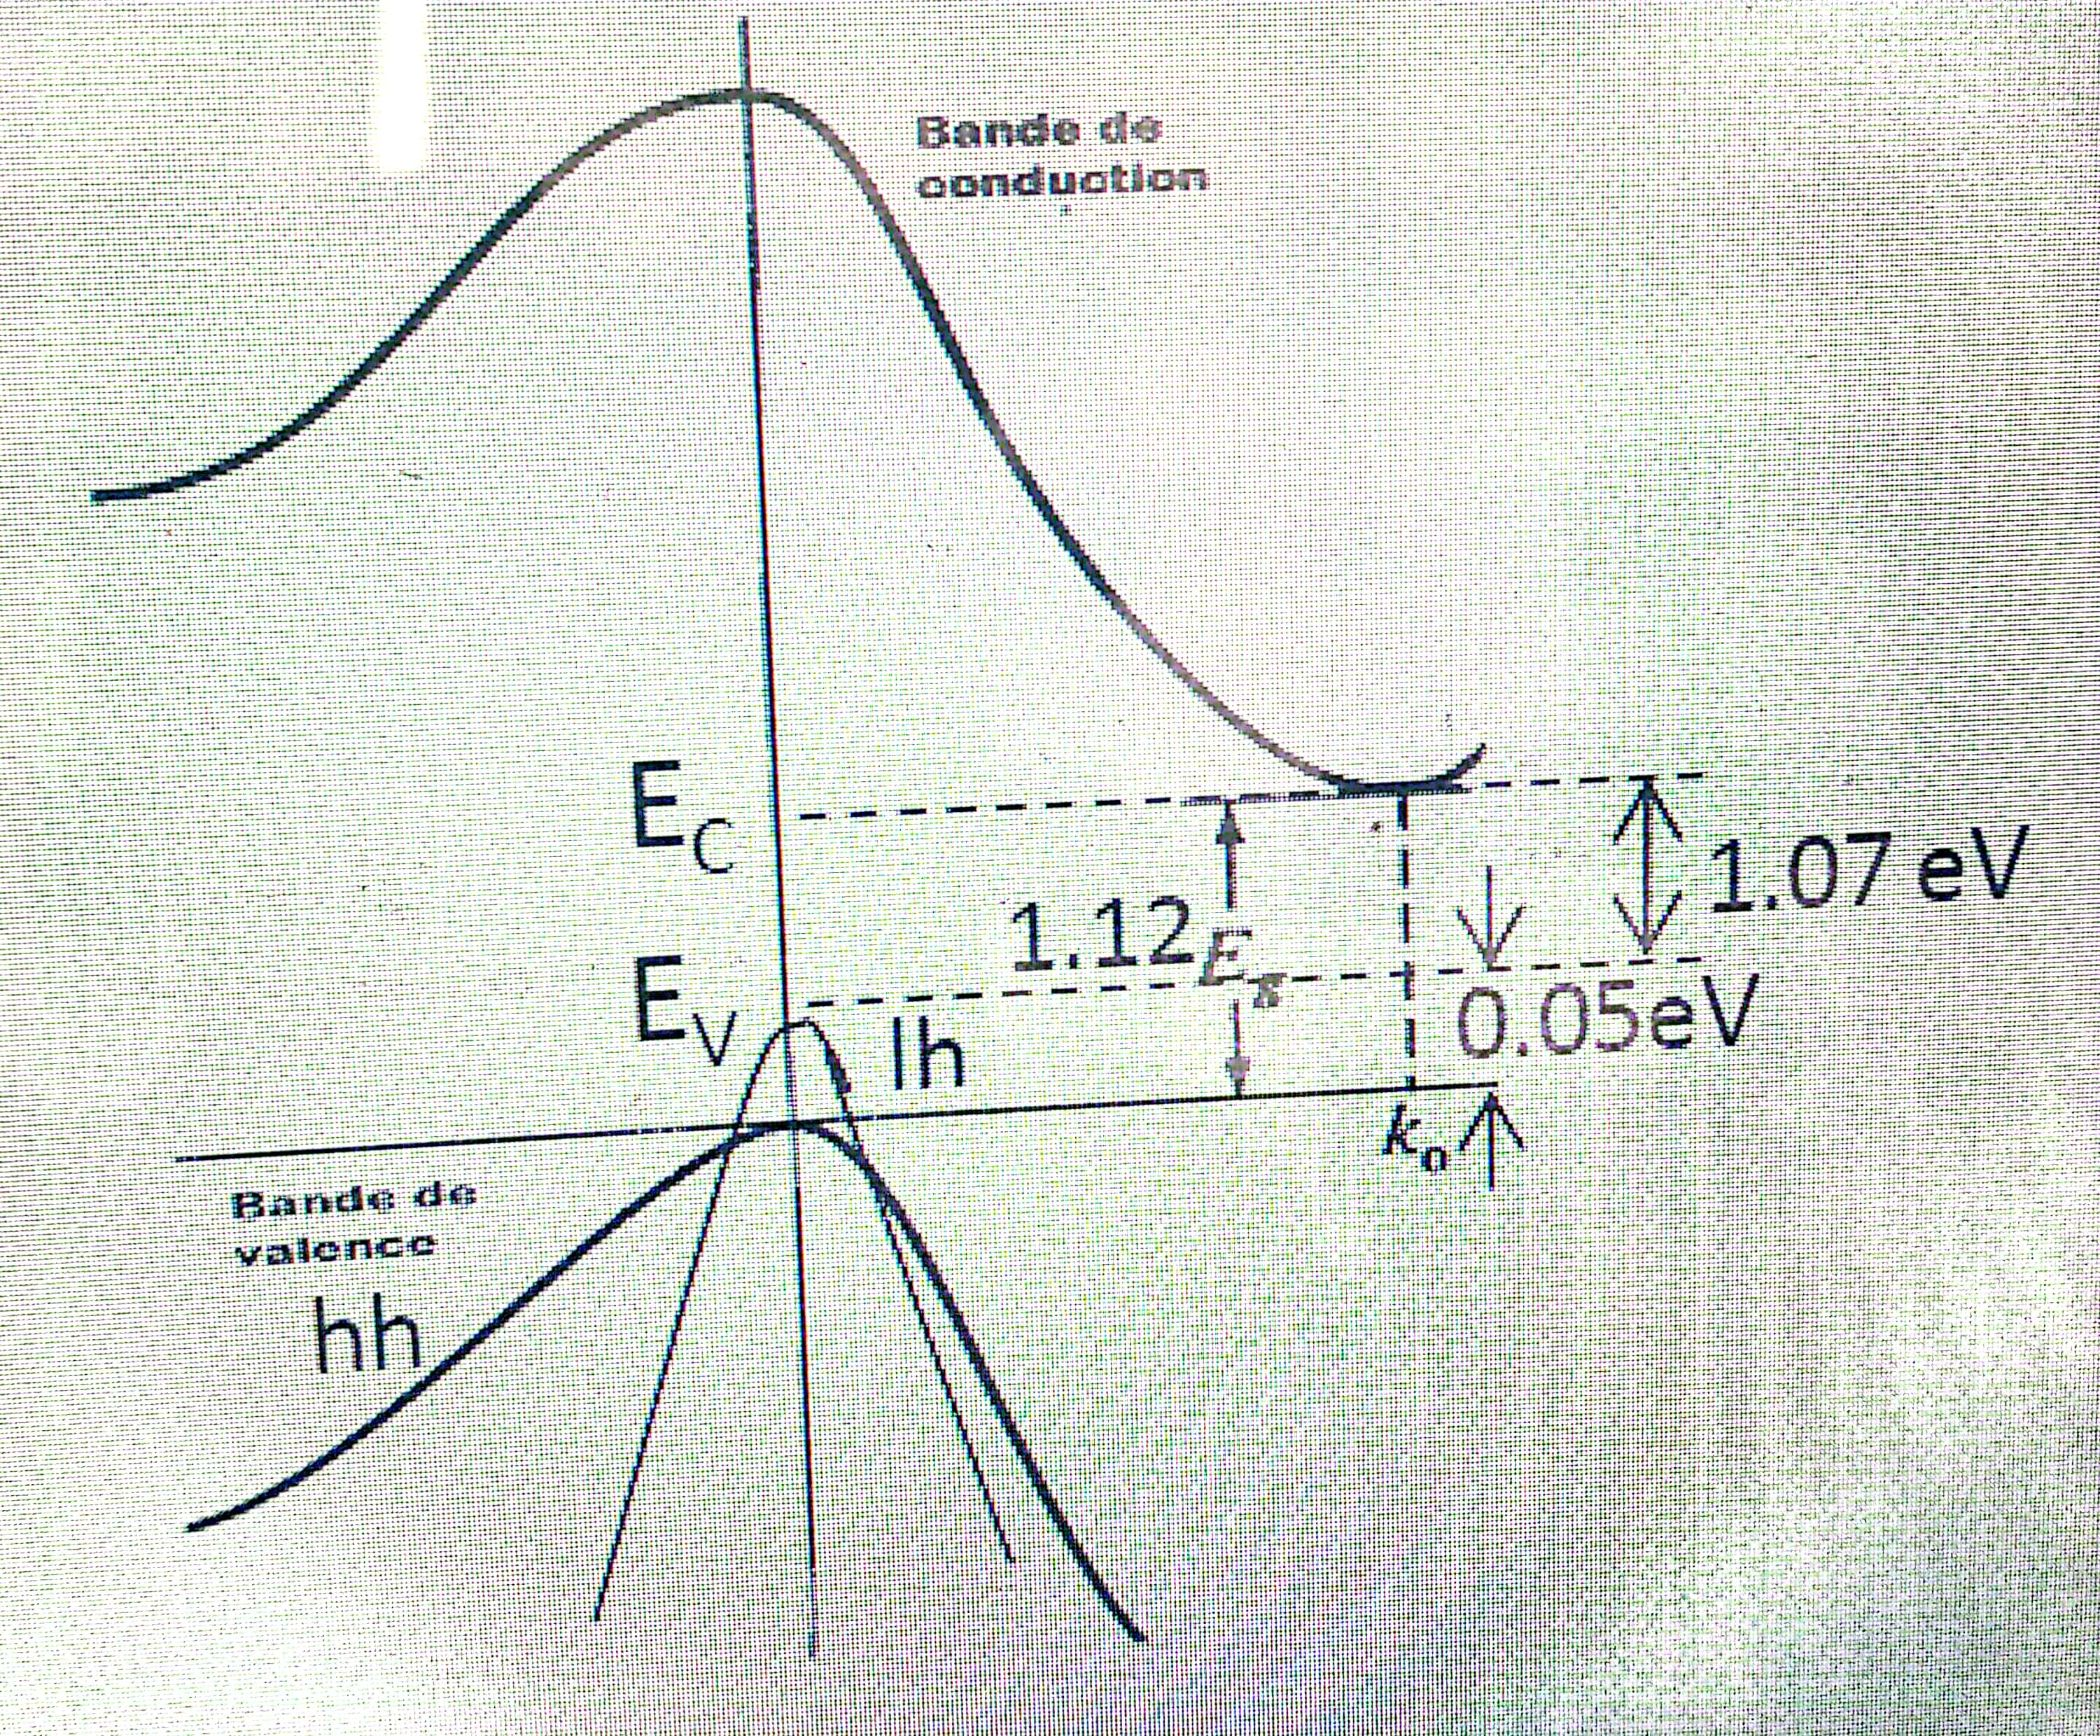
\includegraphics[width=0.55\textwidth]{images/semi_conducteurs/bandes_energie.png}\\[4pt]
{\small\itshape Structure de bandes d'un semi-conducteur : bande de conduction (haut) et bande de valence (bas), séparées par le gap $E_g$.}
\end{center}

\begin{center}

\includegraphics[width=0.6\textwidth]{images/semi_conducteurs/sc-006-000.png}\\[4pt]
{\small\itshape Classification des solides : conducteur, semi-conducteur et isolant selon la largeur du gap.}
\end{center}

\textbf{2.} Classification :
\begin{itemize}[nosep]
  \item Cu : $E_g \approx 0$ $\to$ \textbf{conducteur} (les bandes se chevauchent).
  \item Si : $E_g = \qty{1.12}{eV}$ $\to$ \textbf{semi-conducteur}.
  \item SiO$_2$ : $E_g \approx \qty{9}{eV}$ $\to$ \textbf{isolant}.
\end{itemize}

\textbf{3.} Dans un semi-conducteur, quand $T$ augmente, l'agitation thermique permet à plus d'électrons de franchir le gap, créant davantage de porteurs ($n$ et $p$ augmentent en $\e^{-E_g/2k_BT}$). La conductivité $\sigma = e(n\mu_n + p\mu_p)$ augmente malgré la légère diminution des mobilités. Dans un métal, le nombre de porteurs est constant, et les collisions avec le réseau augmentent, réduisant la mobilité (résistivité croissante).

\textbf{4.} On utilise l'approximation $n_i \propto T^{3/2}\e^{-E_g/(2k_BT)}$ :
\[
\frac{n_i(400)}{n_i(300)} = \left(\frac{400}{300}\right)^{3/2}\times\frac{\e^{-E_g/(2k_B\times400)}}{\e^{-E_g/(2k_B\times300)}}
\]
Le terme $T^{3/2}$ : $(400/300)^{3/2} = (4/3)^{3/2} \approx 1{,}54$.
Le terme exponentiel avec $E_g = 1{,}12\,\text{eV}$, $k_B = 8{,}617\times10^{-5}\,\text{eV/K}$ :
\[
\frac{E_g}{2k_B}\left(\frac{1}{300}-\frac{1}{400}\right) = \frac{1{,}12}{1{,}723\times10^{-4}}\times\frac{100}{120000} \approx 6503\times8{,}33\times10^{-4} \approx 5{,}42
\]
\[
\frac{n_i(400)}{n_i(300)} \approx 1{,}54\times\e^{5{,}42} \approx 1{,}54\times226 \approx \boxed{348}
\]
À 400\,K, $n_i$ est environ 350 fois plus grande qu'à 300\,K.
\end{boitecorrige}

\subsection*{Exercice 7 - Potentiel de contact et zone de déplétion \niveau{\moyen}}

\begin{boiteexercice}
Une jonction abrupte p-n en silicium ($\varepsilon_r = 11{,}7$, $\varepsilon_0 = \qty{8.85e-12}{F.m^{-1}}$) à 300\,K possède : $N_A = \qty{1e17}{cm^{-3}}$ côté p et $N_D = \qty{1e15}{cm^{-3}}$ côté n. On donne $n_i = \qty{1.5e10}{cm^{-3}}$ et $V_T = k_BT/e = \qty{25.85}{mV}$.
\begin{enumerate}
  \item Calculer la tension de contact $V_0$.
  \item La largeur de la zone de déplétion côté n est $x_n = \sqrt{\dfrac{2\varepsilon V_0}{e}\,\dfrac{N_A}{N_D(N_A+N_D)}}$. Calculer $x_n$ et $x_p = x_n N_D/N_A$.
  \item Calculer le champ électrique maximal $E_{max} = eN_Dx_n/\varepsilon$ (en V/cm).
\end{enumerate}
\end{boiteexercice}

\begin{boitecorrige}
\textbf{1.}
\[
V_0 = V_T\ln\!\left(\frac{N_A N_D}{n_i^2}\right) = 0{,}02585\times\ln\!\left(\frac{10^{17}\times10^{15}}{(1{,}5\times10^{10})^2}\right)
\]
\[
= 0{,}02585\times\ln\!\left(\frac{10^{32}}{2{,}25\times10^{20}}\right) = 0{,}02585\times\ln(4{,}44\times10^{11})
\]
\[
= 0{,}02585\times\ln(4{,}44\times10^{11}) = 0{,}02585\times26{,}8 \approx \boxed{\qty{0.693}{V}}
\]

\textbf{2.} Permittivité absolue : $\varepsilon = \varepsilon_r\varepsilon_0 = 11{,}7\times8{,}85\times10^{-12} = \qty{1.036e-10}{F.m^{-1}}$.

\begin{center}
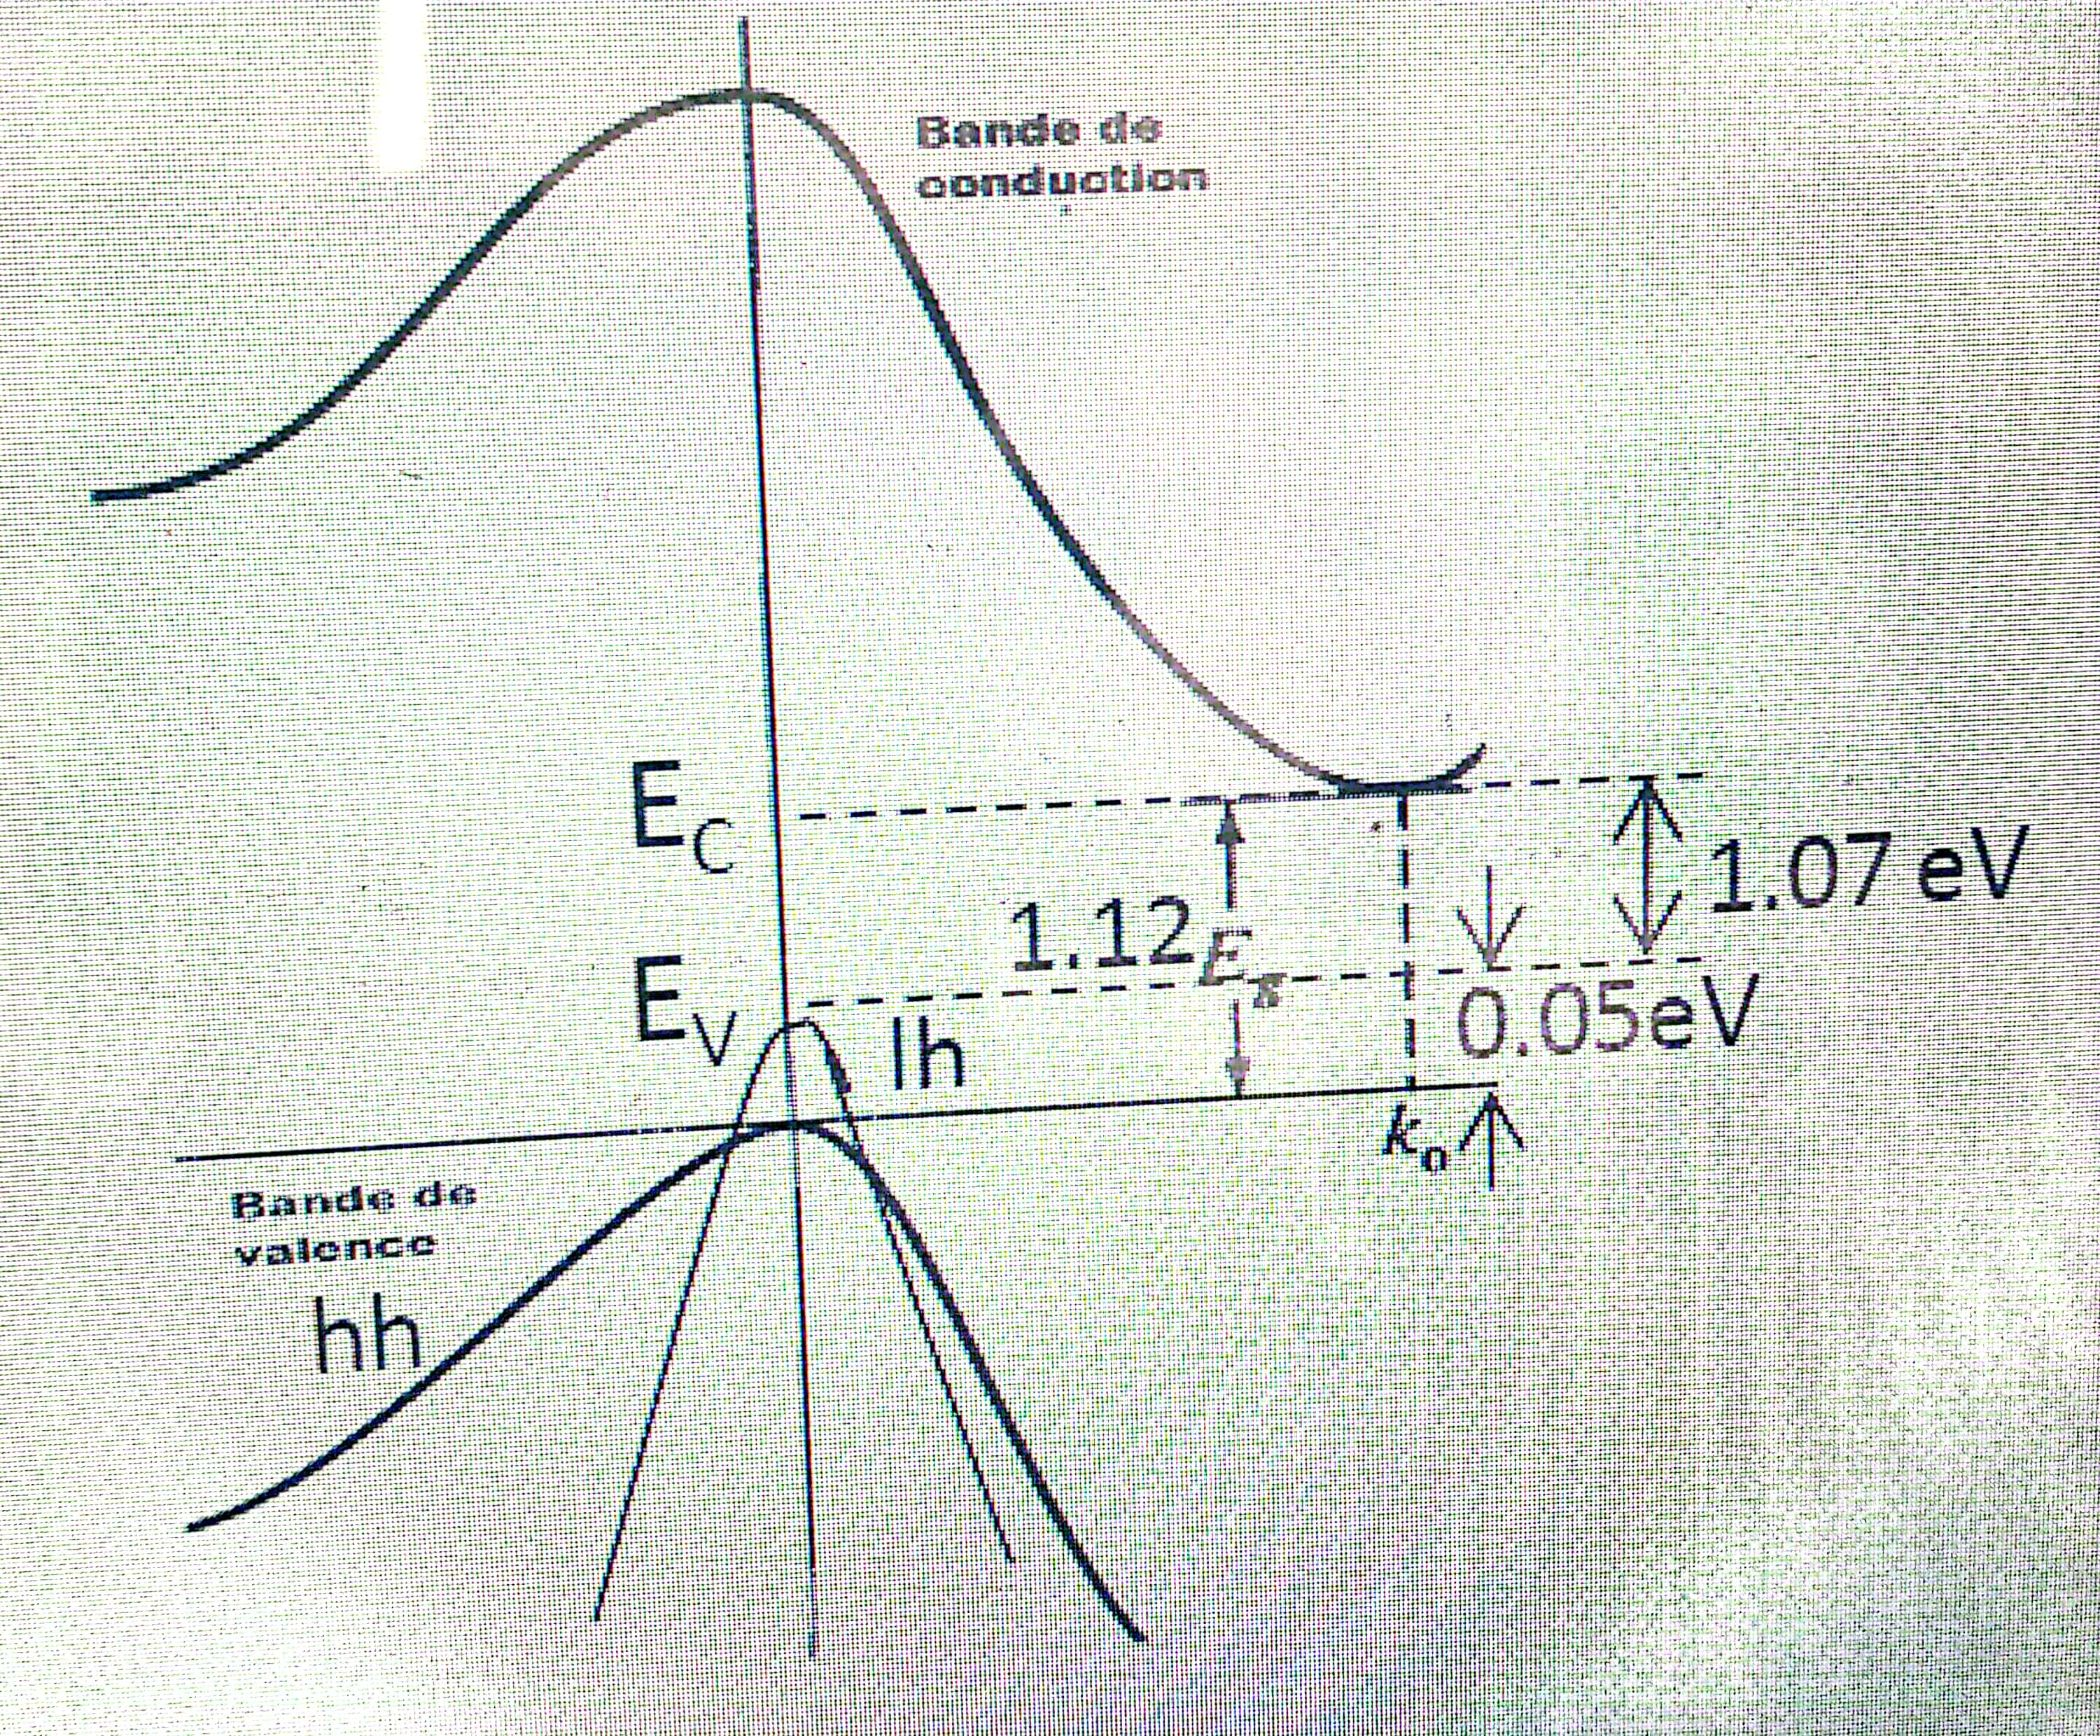
\includegraphics[width=0.7\textwidth]{images/semi_conducteurs/sc-006-001.png}\\[4pt]
{\small\itshape Jonction p-n à l'équilibre : zone de déplétion, champ interne et tension de contact $V_0$.}
\end{center}

Avec $N_D = 10^{15}\,\text{cm}^{-3} = 10^{21}\,\text{m}^{-3}$, $N_A = 10^{17}\,\text{cm}^{-3} = 10^{23}\,\text{m}^{-3}$, $e = \qty{1.6e-19}{C}$ :
\begin{align*}
x_n &= \sqrt{\frac{2\times1{,}036\times10^{-10}\times0{,}693}{1{,}6\times10^{-19}}\,\frac{10^{23}}{10^{21}(10^{23}+10^{21})}}\\
&\approx \sqrt{\frac{1{,}435\times10^{-10}}{1{,}6\times10^{-19}}\,\frac{10^{23}}{1{,}01\times10^{21}\times10^{23}}}\\
&= \sqrt{\frac{1{,}435\times10^{-10}}{1{,}6\times10^{-19}}\times\frac{1}{1{,}01\times10^{21}}}
\approx \sqrt{8{,}87\times10^{-13}} \approx \qty{9.4e-7}{m} = \qty{0.94}{\mu m}
\end{align*}

$x_p = x_n\times N_D/N_A = 0{,}94\times10^{15}/10^{17} = \qty{9.4e-3}{\mu m} = \qty{9.4}{nm}$

\textbf{3.} Champ électrique maximal :
\[
E_{max} = \frac{eN_Dx_n}{\varepsilon} = \frac{1{,}6\times10^{-19}\times10^{21}\times9{,}4\times10^{-7}}{1{,}036\times10^{-10}} \approx \qty{1.45e5}{V.m^{-1}} = \qty{1450}{V.cm^{-1}}
\]
\end{boitecorrige}

\subsection*{Exercice 8 - Équation de Shockley et caractéristique I-V \niveau{\moyen}}

\begin{boiteexercice}
Une diode au silicium à 300\,K a un courant de saturation $I_s = \qty{10}{nA}$ et $V_T = \qty{25.85}{mV}$.
\begin{enumerate}
  \item Rappeler l'équation de Shockley $I = I_s(\e^{V/V_T}-1)$ et ses hypothèses.
  \item Calculer $I$ pour $V = \qty{0.5}{V}$ (direct) et $V = \qty{-5}{V}$ (inverse).
  \item Trouver la tension $V$ telle que $I = \qty{1}{mA}$.
  \item On veut polariser la diode à $I_0 = \qty{5}{mA}$ avec une alimentation $V_{CC} = \qty{5}{V}$. Calculer la résistance de limitation $R$ nécessaire (en supposant $V_D \approx \qty{0.65}{V}$).
\end{enumerate}
\end{boiteexercice}

\begin{boitecorrige}
\textbf{1.} L'équation de Shockley $I = I_s(\e^{V/V_T}-1)$ décrit la caractéristique I-V d'une jonction idéale. Elle repose sur les hypothèses : porteurs minoritaires peu nombreux (faible injection), pas de recombinaison dans la zone de déplétion, jonction abrupte. $V_T = k_BT/e$ est la tension thermique.

\textbf{2.}
\begin{itemize}[nosep]
  \item Polarisation directe $V = \qty{0.5}{V}$ : $\e^{0{,}5/0{,}02585} = \e^{19{,}34} \approx 2{,}50\times10^8$.
  \[
  I = 10\times10^{-9}\times(2{,}50\times10^8 - 1) \approx 10\times10^{-9}\times2{,}50\times10^8 = \qty{2.5}{A}
  \]
  \item Polarisation inverse $V = \qty{-5}{V}$ : $\e^{-5/0{,}02585} = \e^{-193} \approx 0$, donc $I \approx -I_s = \qty{-10}{nA}$.
\end{itemize}

\textbf{3.} Pour $I = \qty{1}{mA}$ :
\[
\e^{V/V_T} = 1 + \frac{I}{I_s} = 1 + \frac{10^{-3}}{10^{-8}} = 10^5
\]
\[
V = V_T\ln(10^5) = 0{,}02585\times5\ln(10) = 0{,}02585\times11{,}51 \approx \boxed{\qty{0.298}{V}}
\]
(En pratique, la tension de seuil réelle du Si est plutôt autour de 0,6--0,7\,V à cause des recombinaisons.)

\textbf{4.} La loi des mailles : $V_{CC} = R\cdot I_0 + V_D$, d'où :
\[
R = \frac{V_{CC} - V_D}{I_0} = \frac{5 - 0{,}65}{5\times10^{-3}} = \frac{4{,}35}{5\times10^{-3}} = \boxed{\qty{870}{\Omega}}
\]
\end{boitecorrige}

\subsection*{Exercice 9 - Transport et mobilité des porteurs \niveau{\moyen}}

\begin{boiteexercice}
Un barreau de silicium de type N ($N_D = \qty{1e16}{cm^{-3}}$, $\mu_n = \qty{1350}{cm^2.V^{-1}.s^{-1}}$, $\mu_p = \qty{480}{cm^2.V^{-1}.s^{-1}}$, $n_i = \qty{1.5e10}{cm^{-3}}$) est soumis à un champ électrique $\vec{E} = \qty{100}{V.cm^{-1}}$.
\begin{enumerate}
  \item Calculer la densité d'électrons $n$ et de trous $p$ à 300\,K.
  \item Calculer la conductivité $\sigma$ et la résistivité $\rho$.
  \item Calculer les vitesses de dérive $v_n = \mu_n E$ et $v_p = \mu_p E$ des électrons et des trous.
  \item Calculer les densités de courant de dérive $J_n = en\mu_n E$ et $J_p = ep\mu_p E$. Quelle est la densité de courant totale ?
\end{enumerate}
\end{boiteexercice}

\begin{boitecorrige}
\textbf{1.} $N_D = \qty{1e16}{cm^{-3}} \gg n_i$ :
\[
n \approx N_D = \qty{1e16}{cm^{-3}} \qquad p = \frac{n_i^2}{n} = \frac{(1{,}5\times10^{10})^2}{10^{16}} = \qty{2.25e4}{cm^{-3}}
\]

\textbf{2.}
\[
\sigma = e(n\mu_n + p\mu_p) \approx en\mu_n = 1{,}6\times10^{-19}\times10^{16}\times1350 = \qty{2.16}{S.cm^{-1}}
\]
\[
\rho = 1/\sigma \approx \qty{0.463}{\Omega.cm}
\]

\textbf{3.} Vitesses de dérive (en valeur absolue) :
\[
v_n = \mu_n E = 1350\times100 = \qty{1.35e5}{cm.s^{-1}} = \qty{1350}{m.s^{-1}}
\]
\[
v_p = \mu_p E = 480\times100 = \qty{4.8e4}{cm.s^{-1}} = \qty{480}{m.s^{-1}}
\]
Les électrons dérivent en sens inverse du champ, les trous dans le sens du champ.

\textbf{4.}
\[
J_n = en\mu_n E = 1{,}6\times10^{-19}\times10^{16}\times1350\times100 = \qty{216}{A.cm^{-2}}
\]
\[
J_p = ep\mu_p E = 1{,}6\times10^{-19}\times2{,}25\times10^4\times480\times100 \approx \qty{1.7e-10}{A.cm^{-2}} \approx 0
\]
\[
J_{total} = J_n + J_p \approx \qty{216}{A.cm^{-2}}
\]
La contribution des trous (porteurs minoritaires) est totalement négligeable.
\end{boitecorrige}

\subsection*{Exercice 10 - Transistor à effet de champ (MOSFET) \niveau{\difficile}}

\begin{boiteexercice}
Un transistor NMOS (canal N) a les paramètres suivants : tension de seuil $V_T = \qty{1}{V}$, transconductance $\mu_n C_{ox} W/L = k = \qty{2}{mA.V^{-2}}$.
\begin{enumerate}
  \item Expliquer le principe de fonctionnement du MOSFET : comment le champ électrique de grille crée-t-il un canal conducteur ?
  \item En régime saturé ($V_{DS} \geq V_{GS} - V_T$), le courant de drain est $I_D = \dfrac{k}{2}(V_{GS}-V_T)^2$. Calculer $I_D$ pour $V_{GS} = \qty{3}{V}$.
  \item En régime linéaire ($V_{DS} < V_{GS}-V_T$), $I_D = k\left[(V_{GS}-V_T)V_{DS} - \dfrac{V_{DS}^2}{2}\right]$. Calculer $I_D$ pour $V_{GS} = \qty{3}{V}$ et $V_{DS} = \qty{0.5}{V}$.
  \item Calculer la résistance du canal $r_{DS} = V_{DS}/I_D$ en régime linéaire avec $V_{DS} \to 0$.
\end{enumerate}
\end{boiteexercice}

\begin{boitecorrige}
\textbf{1.} Dans un MOSFET à canal N, l'application d'une tension positive $V_{GS}$ sur la grille crée un champ électrique qui attire les électrons minoritaires (substrat p) vers l'interface oxyde-silicium. Pour $V_{GS} > V_T$, une couche d'inversion (canal N) se forme entre source et drain. Le courant $I_D$ est contrôlé par $V_{GS}$, d'où l'effet de champ (FET = Field Effect Transistor).

\textbf{2.} Régime saturé avec $V_{GS} = \qty{3}{V}$, $V_T = \qty{1}{V}$ :
\[
I_D = \frac{k}{2}(V_{GS}-V_T)^2
   = \frac{2\times10^{-3}}{2}(3-1)^2
   = 10^{-3}\times4 = \qty{4}{mA}
\]

\textbf{3.} Régime linéaire avec $V_{GS} = \qty{3}{V}$, $V_{DS} = \qty{0.5}{V}$ (vérifions : $V_{DS} = 0{,}5 < V_{GS}-V_T = 2$ : oui, régime linéaire) :
\begin{align*}
I_D &= 2\times10^{-3}\times\left[(3-1)\times0{,}5 - \frac{(0{,}5)^2}{2}\right]\\
    &= 2\times10^{-3}\times(1 - 0{,}125)\\
    &= 2\times10^{-3}\times0{,}875 = \qty{1.75}{mA}
\end{align*}

\textbf{4.} En régime linéaire pour $V_{DS} \ll V_{GS}-V_T$ :
\[
I_D \approx k(V_{GS}-V_T)V_{DS} \quad\Rightarrow\quad r_{DS} = \frac{V_{DS}}{I_D} = \frac{1}{k(V_{GS}-V_T)} = \frac{1}{2\times10^{-3}\times2} = \qty{250}{\ohm}
\]
Plus $V_{GS}$ est élevé, plus le canal est ouvert (résistance faible).
\end{boitecorrige}

\ifdefined\inMainDoc\else\end{document}\fi


% ================================================================
%  UE 12 : PROGRAMMATION EN PYTHON
% ================================================================
\newpage
\thispagestyle{empty}
\begin{tikzpicture}[remember picture, overlay]
  \fill[gray!12] ([xshift=1.5cm, yshift=3cm]current page.south west)
    rectangle ([xshift=-1.5cm, yshift=-3cm]current page.north east);
  \draw[line width=3pt] ([xshift=1.5cm,yshift=-3cm]current page.north west)
    -- ([xshift=-1.5cm,yshift=-3cm]current page.north east);
  \draw[line width=3pt] ([xshift=1.5cm,yshift=3cm]current page.south west)
    -- ([xshift=-1.5cm,yshift=3cm]current page.south east);
  \node[align=center] at (current page.center) {%
    {\fontsize{30}{38}\bfseries\selectfont PROGRAMMATION EN PYTHON}\\[1.2cm]
    {\large\itshape NumPy - Matplotlib - SciPy}\\[0.4cm]
    {\large\itshape Calcul scientifique et visualisation}\\[1.8cm]
    {\normalsize Licence 2 - UE 12}
  };
  \node[anchor=south west] at ([xshift=2cm,yshift=2cm]current page.south west)
    {\large\bfseries UE 12};
\end{tikzpicture}
\newpage

\addcontentsline{toc}{section}{PROGRAMMATION EN PYTHON}
\ifdefined\inMainDoc\else
\documentclass[12pt,a4paper]{article}
% ================================================================
%  PRÉAMBULE COMMUN - ANNALES CORRIGÉES
%  Université de Kara - FaST - Licence Fondamentale MPC
%  Design optimisé impression noir et blanc
% ================================================================

% -- ENCODAGE & LANGUE --
\usepackage[utf8]{inputenc}
\usepackage[T1]{fontenc}
\usepackage[french]{babel}
\usepackage{lmodern}
\usepackage{microtype}

% -- MISE EN PAGE --
\usepackage[a4paper, top=2.8cm, bottom=2.5cm, left=2.5cm, right=2.5cm, headheight=14pt]{geometry}
\usepackage{setspace}
\setstretch{1.2}
\usepackage{parskip}
\setlength{\parindent}{1.2em}
\setlength{\parskip}{4pt}

% -- MATHS --
\usepackage{amsmath, amssymb, mathtools, amsthm}
\usepackage{mathrsfs}
\usepackage{dsfont}
\usepackage{bm}
\usepackage{cancel}
\usepackage{textcomp}
% Définition de \oiint (intégrale de surface fermée) sans package supplémentaire
\newcommand{\oiint}{\mathop{\iint\!\!\!\!\!\!\!\bigcirc}\limits}

% -- PHYSIQUE & CHIMIE --
\usepackage{physics}
\usepackage{siunitx}
% Lorsque physics est chargé, siunitx omet \qty. On le restaure ici :
\AtBeginDocument{\RenewCommandCopy\qty\SI}
\sisetup{locale = FR, detect-all, output-decimal-marker={,}}
% Commande de substitution pour les unités posant problème avec pdflatex
% (ohm, degreeCelsius, micro, angstrom, percent utilisent des caractères non-ASCII)
\newcommand{\qtyohm}[1]{\ensuremath{\num{#1}\,\Omega}}
\newcommand{\qtydegc}[1]{\ensuremath{\num{#1}\,{}^\circ\text{C}}}
\newcommand{\qtyangstrom}[1]{\ensuremath{\num{#1}\,\text{\AA}}}
\newcommand{\qtypercent}[1]{\ensuremath{\num{#1}\,\%}}
\newcommand{\qtyum}[1]{\ensuremath{\num{#1}\,\mu\text{m}}}
\usepackage[version=4]{mhchem}

% -- GRAPHISMES --
\usepackage{graphicx}
\usepackage{float}
\usepackage{caption}
\usepackage{subcaption}
\usepackage{wrapfig}
\usepackage{tikz}
\usetikzlibrary{calc, arrows.meta, patterns, shapes.geometric}
\usepackage{pgfplots}
\pgfplotsset{compat=1.18}

% -- TABLEAUX --
\usepackage{booktabs}
\usepackage{array}
\usepackage{tabularx}
\usepackage{multirow}

% -- LISTES --
\usepackage{enumitem}
\setlist[enumerate]{topsep=3pt, itemsep=2pt, parsep=0pt}
\setlist[itemize]{topsep=3pt, itemsep=2pt, parsep=0pt, label={.}}

% -- BOÎTES (noir et blanc) --
\usepackage{mdframed}
\usepackage{tcolorbox}
\tcbuselibrary{skins, breakable, theorems}

% Boîte EXERCICE : encadré avec filet épais, fond blanc
\newmdenv[
  linewidth=1.2pt,
  linecolor=black,
  roundcorner=3pt,
  skipabove=10pt,
  skipbelow=6pt,
  innertopmargin=8pt,
  innerbottommargin=8pt,
  innerleftmargin=10pt,
  innerrightmargin=10pt,
  backgroundcolor=white,
  frametitle={\bfseries\small Exercice},
  frametitlealignment=\raggedright,
  frametitleaboveskip=4pt,
  frametitlebelowskip=4pt,
]{boiteexercice}

% Boîte CORRIGÉ : fond gris très clair + filet fin
\newmdenv[
  linewidth=0.6pt,
  linecolor=black,
  leftline=true,
  rightline=false,
  topline=false,
  bottomline=false,
  linecolor=black,
  innerleftmargin=12pt,
  innerrightmargin=8pt,
  innertopmargin=6pt,
  innerbottommargin=6pt,
  backgroundcolor=gray!8,
  skipabove=4pt,
  skipbelow=8pt,
]{boitecorrige}

% Boîte RÉSUMÉ DE COURS : double encadré
\newmdenv[
  linewidth=0.8pt,
  linecolor=black,
  roundcorner=2pt,
  backgroundcolor=gray!12,
  innertopmargin=10pt,
  innerbottommargin=10pt,
  innerleftmargin=12pt,
  innerrightmargin=12pt,
  skipabove=12pt,
  skipbelow=8pt,
]{boiteresume}

% Boîte ATTENTION/REMARQUE : barre gauche épaisse
\newmdenv[
  leftline=true,
  rightline=false,
  topline=false,
  bottomline=false,
  linewidth=3pt,
  linecolor=black,
  backgroundcolor=gray!5,
  innerleftmargin=12pt,
  innerrightmargin=8pt,
  innertopmargin=5pt,
  innerbottommargin=5pt,
  skipabove=6pt,
  skipbelow=6pt,
]{boiteremarque}

% -- DIFFICULTÉ DES EXERCICES --
\newcommand{\facile}{$\star$}
\newcommand{\moyen}{$\star\!\star$}
\newcommand{\difficile}{$\star\!\star\!\star$}
\newcommand{\niveau}[1]{\hfill\textbf{#1}\hspace{2pt}}

% -- EN-TÊTES ET PIEDS DE PAGE --
\usepackage{fancyhdr}
\pagestyle{fancy}
\fancyhf{}
\renewcommand{\headrulewidth}{0.5pt}
\renewcommand{\footrulewidth}{0.3pt}

% -- HYPERLIENS --
\usepackage[hidelinks]{hyperref}
\hypersetup{
    colorlinks=false,
    pdftitle={Annale Corrigée - Licence MPC - Université de Kara}
}

% -- TITRES --
\usepackage{titlesec}
\titleformat{\section}{\Large\bfseries}{\thesection.}{0.8em}{}[\vspace{2pt}\hrule\vspace{4pt}]
\titleformat{\subsection}{\large\bfseries}{\thesubsection.}{0.7em}{}
\titleformat{\subsubsection}{\normalsize\bfseries}{\thesubsubsection.}{0.6em}{}

% -- THÉORÈMES --
\theoremstyle{definition}
\newtheorem{defn}{Définition}[section]
\newtheorem{prop}{Propriété}[section]
\newtheorem{thm}{Théorème}[section]
\newtheorem{corol}{Corollaire}[section]
\newtheorem{exemple}{Exemple}[section]

% -- COMMANDES MATHÉMATIQUES UTILES --
\newcommand{\vect}[1]{\overrightarrow{#1}}
\newcommand{\R}{\mathbb{R}}
\newcommand{\N}{\mathbb{N}}
\newcommand{\Z}{\mathbb{Z}}
\newcommand{\C}{\mathbb{C}}
\renewcommand{\d}{\mathrm{d}}
\newcommand{\deriv}[2]{\dfrac{\d #1}{\d #2}}
\newcommand{\dpart}[2]{\dfrac{\partial #1}{\partial #2}}
\newcommand{\rot}{\overrightarrow{\mathrm{rot}}\,}
\renewcommand{\div}{\mathrm{div}\,}
\renewcommand{\grad}{\overrightarrow{\mathrm{grad}}\,}
\newcommand{\e}{\mathrm{e}}
\newcommand{\ii}{\mathrm{i}}
\renewcommand{\Tr}{\mathrm{Tr}}

% Numérotation des équations par section
\numberwithin{equation}{section}

% -- RÉSULTATS ENCADRÉS --
\newcommand{\res}[1]{\[\boxed{#1}\]}

% -- REMARQUE INLINE --
\newcommand{\rmq}[1]{\begin{boiteremarque}\textbf{Remarque.} #1\end{boiteremarque}}

% -- MISE EN VALEUR DU RÉSULTAT FINAL --
\newcommand{\reponse}[1]{%
  \begin{center}
    \fbox{\begin{minipage}{0.92\textwidth}\centering #1\end{minipage}}
  \end{center}%
}


\lhead{\small\textit{Programmation Python - Licence 2}}
\rhead{\small\textit{FaST, Université de Kara}}
\cfoot{\thepage}

\usepackage{listings}
\lstset{
  language=Python,
  basicstyle=\ttfamily\small,
  keywordstyle=\bfseries,
  commentstyle=\itshape,
  stringstyle=\ttfamily,
  numbers=left,
  numberstyle=\tiny,
  numbersep=8pt,
  frame=single,
  breaklines=true,
  tabsize=4,
  showstringspaces=false,
  literate={é}{{\'{e}}}1 {è}{{\`{e}}}1 {ê}{{\^{e}}}1
           {à}{{\`a}}1 {ù}{{\`u}}1 {î}{{\^i}}1 {ô}{{\^o}}1
           {ç}{{\c{c}}}1
}

\begin{document}
\fi

\begin{center}
  {\LARGE\bfseries PROGRAMMATION EN PYTHON}\\[0.3cm]
  {\normalsize Licence 2 - Mathématiques, Physique et Chimie}\\[0.1cm]
  \rule{0.7\textwidth}{0.8pt}
\end{center}

\section*{Résumé du cours}

\begin{boiteresume}

\textbf{1. Types et variables.} Python est un langage interprété à typage dynamique. Types de base : \texttt{int}, \texttt{float}, \texttt{complex}, \texttt{str}, \texttt{bool}, \texttt{list}, \texttt{tuple}, \texttt{dict}, \texttt{set}.

\textbf{2. Structures de contrôle.}
\begin{lstlisting}
if condition:           # conditionnel
    ...
elif autre:
    ...
else:
    ...

for i in range(n):      # boucle for
    ...

while condition:        # boucle while
    ...
\end{lstlisting}

\textbf{3. Fonctions.}
\begin{lstlisting}
def nom_fonction(param1, param2, defaut=0):
    """Docstring."""
    return resultat
\end{lstlisting}

\textbf{4. Bibliothèques scientifiques.}
\begin{itemize}[nosep]
  \item \texttt{numpy} : tableaux numériques, algèbre linéaire, fonctions mathématiques.
  \item \texttt{matplotlib} : tracé de courbes (\texttt{plt.plot}, \texttt{plt.show}).
  \item \texttt{scipy} : intégration, optimisation, statistiques.
\end{itemize}

\textbf{5. Listes et compréhensions.} \texttt{[f(x) for x in liste if condition]} crée une liste en une ligne. Les tableaux NumPy (\texttt{np.array}) permettent des opérations vectorisées (plus rapides que les boucles).

\end{boiteresume}

\newpage
\section{Bases du langage}

\subsection*{Exercice 1 - Variables et opérations \niveau{\facile}}

\begin{boiteexercice}
Écrire un programme Python qui :
\begin{enumerate}
  \item Demande à l'utilisateur deux réels $a$ et $b$.
  \item Affiche leurs somme, différence, produit et rapport.
  \item Résout l'équation $ax^2 + bx + c = 0$ (en demandant aussi $c$) en affichant toutes les racines complexes.
\end{enumerate}
\end{boiteexercice}

\begin{boitecorrige}
\begin{lstlisting}
import cmath  # pour les racines complexes

# Partie 1 : operations de base
a = float(input("Entrez a : "))
b = float(input("Entrez b : "))

print(f"Somme      : {a} + {b} = {a + b}")
print(f"Difference : {a} - {b} = {a - b}")
print(f"Produit    : {a} * {b} = {a * b}")
if b != 0:
    print(f"Rapport    : {a} / {b} = {a / b:.4f}")
else:
    print("Division par zero impossible.")

# Partie 2 : trinome du second degre
print("\n- Resolution du trinome ax^2 + bx + c -")
c = float(input("Entrez c : "))

if a == 0:
    print("Ce n'est pas un trinome (a = 0).")
else:
    delta = b**2 - 4*a*c
    x1 = (-b + cmath.sqrt(delta)) / (2*a)
    x2 = (-b - cmath.sqrt(delta)) / (2*a)
    if delta > 0:
        print(f"Deux racines reelles : x1 = {x1.real:.4f}, x2 = {x2.real:.4f}")
    elif delta == 0:
        print(f"Racine double : x = {x1.real:.4f}")
    else:
        print(f"Racines complexes : x1 = {x1}, x2 = {x2}")
\end{lstlisting}
\end{boitecorrige}

\section{Calcul scientifique avec NumPy et Matplotlib}

\subsection*{Exercice 2 - Tracé de fonctions \niveau{\facile}}

\begin{boiteexercice}
Tracer sur le même graphique les fonctions $f(x)=\sin(x)$, $g(x)=\cos(x)$ et $h(x)=\sin(2x)$ pour $x\in[0,2\pi]$ avec une légende, un titre et des labels d'axes. Ajouter une grille.
\end{boiteexercice}

\begin{boitecorrige}
\begin{lstlisting}
import numpy as np
import matplotlib.pyplot as plt

x = np.linspace(0, 2*np.pi, 500)

plt.figure(figsize=(9, 5))
plt.plot(x, np.sin(x),   label=r'$\sin(x)$',   linewidth=2)
plt.plot(x, np.cos(x),   label=r'$\cos(x)$',   linewidth=2, linestyle='--')
plt.plot(x, np.sin(2*x), label=r'$\sin(2x)$',  linewidth=2, linestyle=':')

plt.axhline(0, color='black', linewidth=0.8)
plt.xlabel('$x$ (radians)', fontsize=12)
plt.ylabel('Valeur', fontsize=12)
plt.title('Fonctions trigonometriques', fontsize=14)
plt.legend(fontsize=12)
plt.grid(True, alpha=0.4)
plt.xticks([0, np.pi/2, np.pi, 3*np.pi/2, 2*np.pi],
           ['0', r'$\pi/2$', r'$\pi$', r'$3\pi/2$', r'$2\pi$'])
plt.tight_layout()
plt.show()
\end{lstlisting}

\texttt{np.linspace(0, 2*np.pi, 500)} génère 500 points régulièrement espacés entre 0 et $2\pi$. Les opérations NumPy (\texttt{np.sin}, \texttt{np.cos}) s'appliquent vectoriellement à tous les points simultanément.
\end{boitecorrige}

\subsection*{Exercice 3 - Méthodes numériques \niveau{\moyen}}

\begin{boiteexercice}
\begin{enumerate}
  \item Implémenter la méthode de la bissection pour trouver la racine de $f(x)=x^3-x-2$ sur $[1,2]$.
  \item Implémenter la méthode d'Euler pour résoudre $y'=y\sin(x)$, $y(0)=1$ sur $[0,5]$. Comparer avec la solution exacte $y(x)=\e^{1-\cos x}$.
\end{enumerate}
\end{boiteexercice}

\begin{boitecorrige}
\textbf{1. Méthode de la bissection :}
\begin{lstlisting}
def bissection(f, a, b, tol=1e-8, max_iter=100):
    """Trouve la racine de f sur [a,b] par bissection."""
    if f(a) * f(b) > 0:
        raise ValueError("f(a) et f(b) doivent etre de signes opposes.")
    for _ in range(max_iter):
        c = (a + b) / 2
        if abs(f(c)) < tol or (b - a) / 2 < tol:
            return c
        if f(a) * f(c) < 0:
            b = c
        else:
            a = c
    return (a + b) / 2

f = lambda x: x**3 - x - 2
racine = bissection(f, 1, 2)
print(f"Racine : x = {racine:.8f}")  # x ~= 1.52137971
\end{lstlisting}

\textbf{2. Méthode d'Euler :}
\begin{lstlisting}
import numpy as np
import matplotlib.pyplot as plt

# Methode d'Euler
def euler(f, y0, x0, xf, n):
    h = (xf - x0) / n
    x = np.linspace(x0, xf, n+1)
    y = np.zeros(n+1)
    y[0] = y0
    for i in range(n):
        y[i+1] = y[i] + h * f(x[i], y[i])
    return x, y

f = lambda x, y: y * np.sin(x)
x_euler, y_euler = euler(f, 1, 0, 5, 200)

# Solution exacte
x_exact = np.linspace(0, 5, 1000)
y_exact = np.exp(1 - np.cos(x_exact))

plt.plot(x_euler, y_euler, label="Euler (n=200)", linestyle='--')
plt.plot(x_exact, y_exact, label="Solution exacte")
plt.legend(); plt.grid(True); plt.show()
\end{lstlisting}
\end{boitecorrige}

\subsection*{Exercice 4 - Algèbre linéaire avec NumPy \niveau{\moyen}}

\begin{boiteexercice}
Résoudre le système $A\vec{x}=\vec{b}$ avec :
\[
A = \begin{pmatrix}2&1&-1\\-3&-1&2\\-2&1&2\end{pmatrix}, \quad \vec{b} = \begin{pmatrix}8\\-11\\-3\end{pmatrix}
\]
en utilisant \texttt{numpy.linalg.solve}. Vérifier la solution, calculer $\det(A)$ et les valeurs propres de $A$.
\end{boiteexercice}

\begin{boitecorrige}
\begin{lstlisting}
import numpy as np

A = np.array([[2, 1, -1],
              [-3, -1, 2],
              [-2, 1, 2]], dtype=float)

b = np.array([8, -11, -3], dtype=float)

# Resolution du systeme
x = np.linalg.solve(A, b)
print(f"Solution : x = {x}")  # x = [2, 3, -1]

# Verification : A @ x doit etre egale a b
residuel = np.linalg.norm(A @ x - b)
print(f"Residuel ||Ax - b|| = {residuel:.2e}")

# Determinant
det = np.linalg.det(A)
print(f"det(A) = {det:.4f}")

# Valeurs propres
valeurs_propres, vecteurs_propres = np.linalg.eig(A)
print(f"Valeurs propres : {valeurs_propres}")
\end{lstlisting}

La solution est $x_1=2$, $x_2=3$, $x_3=-1$. \texttt{np.linalg.solve} utilise la décomposition LU, ce qui est bien plus efficace que l'inversion de matrice (\texttt{np.linalg.inv}).
\end{boitecorrige}

\subsection*{Exercice 5 - Traitement de données et statistiques \niveau{\difficile}}

\begin{boiteexercice}
On dispose d'une série de mesures de la résistance d'un conducteur à différentes températures :

\begin{center}
\begin{tabular}{c|cccccc}
$T$ (°C) & 20 & 40 & 60 & 80 & 100 & 120\\
\hline
$R$ ($\Omega$) & 10.2 & 11.1 & 12.0 & 12.8 & 13.9 & 14.7
\end{tabular}
\end{center}

\begin{enumerate}
  \item Calculer la moyenne, l'écart-type et le coefficient de variation de $R$.
  \item Effectuer une régression linéaire $R = aT + b$ par la méthode des moindres carrés (\texttt{numpy.polyfit}).
  \item Estimer la résistance à $T = \qtydegc{150}$.
  \item Tracer les données et la droite de régression.
\end{enumerate}
\end{boiteexercice}

\begin{boitecorrige}
\begin{lstlisting}
import numpy as np
import matplotlib.pyplot as plt

T = np.array([20, 40, 60, 80, 100, 120], dtype=float)
R = np.array([10.2, 11.1, 12.0, 12.8, 13.9, 14.7])

# 1. Statistiques descriptives
print(f"Moyenne de R  : {np.mean(R):.3f} Ohm")
print(f"Ecart-type    : {np.std(R, ddof=1):.3f} Ohm")
print(f"Coeff. variation : {100*np.std(R,ddof=1)/np.mean(R):.1f} %")

# 2. Regression lineaire
coeffs = np.polyfit(T, R, 1)
a, b = coeffs
print(f"\nRegression : R = {a:.4f} * T + {b:.4f}")

# Coefficient de correlation
r = np.corrcoef(T, R)[0, 1]
print(f"Coefficient de correlation r = {r:.4f}")

# 3. Estimation a T = 150 degC
T_pred = 150
R_pred = a * T_pred + b
print(f"\nEstimation a {T_pred} degC : R = {R_pred:.2f} Ohm")

# 4. Trace
T_fit = np.linspace(0, 160, 100)
R_fit = a * T_fit + b

plt.scatter(T, R, color='black', zorder=5, label='Mesures')
plt.plot(T_fit, R_fit, label=f'Regression: R={a:.3f}T+{b:.3f}')
plt.xlabel('Temperature (degC)'); plt.ylabel('Resistance (Ohm)')
plt.title('Resistance vs Temperature')
plt.legend(); plt.grid(True); plt.show()
\end{lstlisting}

Résultats : $a \approx \ensuremath{\num{0.045}\,\Omega/{}^\circ\text{C}}$, $b \approx \qty{9.28}{\Omega}$, $r \approx 0{,}9997$. La linéarité est excellente. À 150°C, $R\approx\qty{16.0}{\Omega}$.
\end{boitecorrige}

\section{Structures de données et algorithmes}

\subsection*{Exercice 6 - Listes, tri et compréhension \niveau{\facile}}

\begin{boiteexercice}
\begin{enumerate}
  \item Créer une liste des carrés des entiers de 1 à 20 en utilisant une compréhension de liste.
  \item Filtrer les éléments pairs de cette liste.
  \item Trier une liste de mots par longueur (puis alphabétiquement en cas d'égalité) : \texttt{mots = ["chat", "python", "code", "AI", "Numpy", "ax"]}.
  \item Écrire une fonction qui recherche un élément dans une liste triée par l'algorithme de \emph{recherche dichotomique}.
\end{enumerate}
\end{boiteexercice}

\begin{boitecorrige}
\begin{lstlisting}
# 1. Comprehension de liste : carres
carres = [n**2 for n in range(1, 21)]
print("Carres:", carres)

# 2. Filtrage des elements pairs
pairs = [x for x in carres if x % 2 == 0]
print("Carres pairs:", pairs)

# 3. Tri par longueur puis alphabetique
mots = ["chat", "python", "code", "AI", "Numpy", "ax"]
mots_tries = sorted(mots, key=lambda m: (len(m), m.lower()))
print("Mots tries:", mots_tries)
# Resultat: ['AI', 'ax', 'chat', 'code', 'Numpy', 'python']

# 4. Recherche dichotomique
def recherche_dicho(liste, cible):
    """Recherche dichotomique dans une liste triee.
    Retourne l'indice si trouve, -1 sinon."""
    gauche, droite = 0, len(liste) - 1
    while gauche <= droite:
        milieu = (gauche + droite) // 2
        if liste[milieu] == cible:
            return milieu
        elif liste[milieu] < cible:
            gauche = milieu + 1
        else:
            droite = milieu - 1
    return -1

nombres = sorted([3, 7, 1, 15, 9, 4, 12])  # [1, 3, 4, 7, 9, 12, 15]
print(f"Recherche de 9 : indice {recherche_dicho(nombres, 9)}")   # 4
print(f"Recherche de 6 : indice {recherche_dicho(nombres, 6)}")   # -1
\end{lstlisting}

\textbf{Complexité :} La recherche dichotomique a une complexité $O(\log_2 n)$ au lieu de $O(n)$ pour la recherche linéaire. Pour $n = 10^6$ éléments, seulement $\sim 20$ comparaisons suffisent.
\end{boitecorrige}

\subsection*{Exercice 7 - Fonctions récursives \niveau{\moyen}}

\begin{boiteexercice}
\begin{enumerate}
  \item Écrire une fonction récursive calculant $n!$ et une version itérative. Comparer pour $n=10$.
  \item Écrire une fonction récursive pour les nombres de Fibonacci $F_n = F_{n-1}+F_{n-2}$, $F_0=0$, $F_1=1$.
  \item Pourquoi la version naïve de Fibonacci est-elle exponentiellement lente ? Implémenter une version mémoïsée avec un dictionnaire.
  \item Calculer $F_{35}$ avec les deux versions et mesurer le temps avec \texttt{time.time()}.
\end{enumerate}
\end{boiteexercice}

\begin{boitecorrige}
\begin{lstlisting}
import time

# 1. Factorielle
def factorielle_rec(n):
    """Factorielle recursive."""
    if n <= 1:
        return 1
    return n * factorielle_rec(n - 1)

def factorielle_iter(n):
    """Factorielle iterative."""
    result = 1
    for i in range(2, n + 1):
        result *= i
    return result

print(f"10! (recursif)  = {factorielle_rec(10)}")
print(f"10! (iteratif)  = {factorielle_iter(10)}")

# 2. Fibonacci naif (exponentiel)
def fib_naif(n):
    if n <= 1:
        return n
    return fib_naif(n-1) + fib_naif(n-2)

# 3. Fibonacci memoize (lineaire)
def fib_memo(n, cache={}):
    if n in cache:
        return cache[n]
    if n <= 1:
        return n
    cache[n] = fib_memo(n-1, cache) + fib_memo(n-2, cache)
    return cache[n]

# 4. Comparaison de temps
n = 35
t0 = time.time()
res_naif = fib_naif(n)
t1 = time.time()
print(f"F({n}) naif    = {res_naif} en {t1-t0:.3f} s")

t0 = time.time()
res_memo = fib_memo(n)
t1 = time.time()
print(f"F({n}) memoize = {res_memo} en {t1-t0:.6f} s")
\end{lstlisting}

\textbf{Analyse :} La version naïve calcule $\sim 2^{35}$ appels (exponentiel), tandis que la version mémoïsée fait $O(n)$ calculs. Pour $n=35$, la version naïve prend $\sim$ 5 secondes, la mémoïsée $\sim$ 0 ms.
\end{boitecorrige}

\subsection*{Exercice 8 - Lecture et écriture de fichiers \niveau{\facile}}

\begin{boiteexercice}
On dispose d'un fichier texte \texttt{mesures.txt} contenant des lignes de la forme \texttt{t R} (temps et résistance).
\begin{enumerate}
  \item Écrire un programme qui génère ce fichier avec des données simulées ($T = [20, 40, 60, 80, 100]$°C, $R = 10 + 0.05T + \text{bruit}$).
  \item Lire le fichier et extraire les données dans deux listes.
  \item Calculer la moyenne et l'écart-type de $R$ à partir des données lues.
  \item Réécrire un fichier \texttt{resultats.txt} avec les statistiques calculées.
\end{enumerate}
\end{boiteexercice}

\begin{boitecorrige}
\begin{lstlisting}
import numpy as np

# 1. Generation et ecriture du fichier
np.random.seed(42)
T_vals = [20, 40, 60, 80, 100]
R_vals = [10 + 0.05*T + np.random.normal(0, 0.1) for T in T_vals]

with open("mesures.txt", "w") as f:
    f.write("# Temperature(C)  Resistance(Ohm)\n")
    for T, R in zip(T_vals, R_vals):
        f.write(f"{T:.1f}  {R:.4f}\n")

print("Fichier mesures.txt cree.")

# 2. Lecture du fichier
temperatures = []
resistances = []

with open("mesures.txt", "r") as f:
    for ligne in f:
        if ligne.startswith("#"):  # ignorer commentaires
            continue
        parts = ligne.strip().split()
        if len(parts) == 2:
            temperatures.append(float(parts[0]))
            resistances.append(float(parts[1]))

print("Temperatures lues:", temperatures)
print("Resistances lues :", [f"{r:.4f}" for r in resistances])

# 3. Statistiques
R_arr = np.array(resistances)
moyenne = np.mean(R_arr)
ecart_type = np.std(R_arr, ddof=1)
print(f"\nMoyenne R = {moyenne:.4f} Ohm")
print(f"Ecart-type = {ecart_type:.4f} Ohm")

# 4. Ecriture des resultats
with open("resultats.txt", "w") as f:
    f.write("=== Resultats statistiques ===\n")
    f.write(f"Nombre de mesures : {len(resistances)}\n")
    f.write(f"Moyenne R         : {moyenne:.4f} Ohm\n")
    f.write(f"Ecart-type        : {ecart_type:.4f} Ohm\n")
    f.write(f"Min / Max         : {R_arr.min():.4f} / {R_arr.max():.4f} Ohm\n")

print("\nFichier resultats.txt ecrit.")
\end{lstlisting}
\end{boitecorrige}

\subsection*{Exercice 9 - NumPy : tableaux et algèbre linéaire \niveau{\moyen}}

\begin{boiteexercice}
\begin{enumerate}
  \item Créer un tableau NumPy $A$ de taille $3\times3$ représentant la matrice de rotation d'angle $\theta = 45°$.
  \item Calculer $\det(A)$, $A^{-1}$, et les valeurs propres et vecteurs propres de $A$.
  \item Résoudre le système $Ax = b$ avec $b = (1, 0, 1)^T$.
  \item Vérifier que $A^{-1}A = I$ et que la solution satisfait bien $Ax = b$.
\end{enumerate}
Matrice de rotation 3D autour de $z$ :
\[
A = \begin{pmatrix}\cos\theta & -\sin\theta & 0\\\sin\theta & \cos\theta & 0\\0 & 0 & 1\end{pmatrix}
\]
\end{boiteexercice}

\begin{boitecorrige}
\begin{lstlisting}
import numpy as np

theta = np.pi / 4  # 45 degres

# 1. Matrice de rotation
A = np.array([
    [np.cos(theta), -np.sin(theta), 0],
    [np.sin(theta),  np.cos(theta), 0],
    [0,              0,             1]
])
print("Matrice A :")
print(np.round(A, 6))

# 2. Determinant, inverse, valeurs propres
det_A = np.linalg.det(A)
print(f"\ndet(A) = {det_A:.6f}")  # doit valoir 1

A_inv = np.linalg.inv(A)
print("\nA^(-1) :")
print(np.round(A_inv, 6))

vals_propres, vects_propres = np.linalg.eig(A)
print(f"\nValeurs propres : {np.round(vals_propres, 4)}")
# Pour une rotation, les VP sont 1 et exp(+-i*theta)

# 3. Resolution du systeme
b = np.array([1.0, 0.0, 1.0])
x = np.linalg.solve(A, b)
print(f"\nSolution x = {np.round(x, 6)}")

# 4. Verification
identite = np.round(A_inv @ A, 10)
print("\nA^(-1) @ A =")
print(identite)

residuel = np.linalg.norm(A @ x - b)
print(f"\nResidu ||Ax - b|| = {residuel:.2e}")
\end{lstlisting}

\textbf{Résultats attendus :} $\det(A) = 1$ (rotation préserve les volumes), valeurs propres $\{1, \e^{i\pi/4}, \e^{-i\pi/4}\}$, résidu $\approx 10^{-15}$.
\end{boitecorrige}

\subsection*{Exercice 10 - Matplotlib : visualisation et histogramme \niveau{\moyen}}

\begin{boiteexercice}
\begin{enumerate}
  \item Générer $N = 1000$ réalisations d'une variable aléatoire gaussienne $X \sim \mathcal{N}(\mu=5, \sigma=2)$ avec NumPy.
  \item Tracer l'histogramme normalisé (densité de probabilité) et superposer la densité théorique $f(x) = \dfrac{1}{\sigma\sqrt{2\pi}}\e^{-(x-\mu)^2/(2\sigma^2)}$.
  \item Calculer la moyenne et l'écart-type empiriques et les comparer aux valeurs théoriques.
  \item Tracer une figure avec deux sous-graphiques : (a) l'histogramme, (b) la courbe de distribution cumulée empirique (ECDF).
\end{enumerate}
\end{boiteexercice}

\begin{boitecorrige}
\begin{lstlisting}
import numpy as np
import matplotlib.pyplot as plt
from scipy.stats import norm

# 1. Generation des donnees
np.random.seed(42)
mu, sigma = 5, 2
N = 1000
data = np.random.normal(mu, sigma, N)

# 3. Statistiques empiriques
print(f"Moyenne empirique : {data.mean():.3f}  (theorique : {mu})")
print(f"Ecart-type empirique : {data.std():.3f}  (theorique : {sigma})")

# 2. et 4. Graphiques
fig, (ax1, ax2) = plt.subplots(1, 2, figsize=(12, 5))

# Sous-graphique 1 : Histogramme
ax1.hist(data, bins=40, density=True, alpha=0.6,
         color='steelblue', label=f'Histogramme (N={N})')

# Densite theorique
x_theo = np.linspace(data.min(), data.max(), 200)
ax1.plot(x_theo, norm.pdf(x_theo, mu, sigma),
         'r-', linewidth=2,
         label=rf'$\mathcal{{N}}(\mu={mu}, \sigma={sigma})$')
ax1.set_xlabel('x'); ax1.set_ylabel('Densite')
ax1.set_title('Histogramme normalise')
ax1.legend()
ax1.grid(alpha=0.3)

# Sous-graphique 2 : ECDF
data_sorted = np.sort(data)
ecdf = np.arange(1, N+1) / N

ax2.step(data_sorted, ecdf, color='steelblue', label='ECDF empirique')
ax2.plot(x_theo, norm.cdf(x_theo, mu, sigma),
         'r-', linewidth=2, label='CDF theorique')
ax2.set_xlabel('x'); ax2.set_ylabel('P(X <= x)')
ax2.set_title('Fonction de repartition')
ax2.legend()
ax2.grid(alpha=0.3)

plt.tight_layout()
plt.savefig("statistiques.pdf", bbox_inches='tight')
plt.show()
\end{lstlisting}

\textbf{Interprétation :} L'histogramme normalisé (densité) converge vers la densité théorique en $1/\sqrt{N}$. L'ECDF (Empirical Cumulative Distribution Function) permet de visualiser la distribution sans choisir une largeur de bin.
\end{boitecorrige}

\section{Algorithmique et structures de données}

\subsection*{Exercice 11 - Parité et année bissextile \niveau{\facile}}

\begin{boiteexercice}
\begin{enumerate}
  \item Écrire un programme qui demande un entier $n$ à l'utilisateur et affiche s'il est pair ou impair.
  \item Écrire un programme qui demande une année et indique si elle est bissextile. Rappel : une année est bissextile si elle est divisible par 4 mais pas par 100, sauf si elle est divisible par 400.
\end{enumerate}
\end{boiteexercice}

\begin{boitecorrige}
\begin{lstlisting}
# 1. Test de parite
n = int(input("Entrez un entier n : "))
if n % 2 == 0:
    print(f"{n} est pair.")
else:
    print(f"{n} est impair.")

# 2. Annee bissextile
annee = int(input("Entrez une annee : "))
if (annee % 4 == 0 and annee % 100 != 0) or (annee % 400 == 0):
    print(f"{annee} est bissextile.")
else:
    print(f"{annee} n'est pas bissextile.")
\end{lstlisting}

\textbf{Tests :} 2024 (bissextile, divisible par 4 mais pas 100), 1900 (non bissextile, divisible par 100 mais pas 400), 2000 (bissextile, divisible par 400).
\end{boitecorrige}

\subsection*{Exercice 12 - PGCD, PPCM et décomposition binaire \niveau{\moyen}}

\begin{boiteexercice}
\begin{enumerate}
  \item Écrire une fonction \texttt{pgcd(a, b)} utilisant l'algorithme d'Euclide, puis une fonction \texttt{ppcm(a, b)} qui en déduit le PPCM via la relation $a \times b = \mathrm{pgcd}(a,b) \times \mathrm{ppcm}(a,b)$.
  \item Écrire une fonction \texttt{binaire(n)} qui retourne la représentation binaire (chaîne de caractères) d'un entier positif sans utiliser \texttt{bin()}.
  \item Tester avec $a = 84$, $b = 60$ et $n = 77$.
\end{enumerate}
\end{boiteexercice}

\begin{boitecorrige}
\begin{lstlisting}
def pgcd(a, b):
    """Algorithme d'Euclide iteratif."""
    while b != 0:
        a, b = b, a % b
    return a

def ppcm(a, b):
    """PPCM via la relation a*b = pgcd(a,b) * ppcm(a,b)."""
    if a == 0 or b == 0:
        return 0
    return abs(a * b) // pgcd(a, b)

def binaire(n):
    """Decomposition binaire d'un entier positif."""
    if n == 0:
        return "0"
    bits = []
    while n > 0:
        bits.append(str(n % 2))
        n //= 2
    return "".join(reversed(bits))

# Tests
a, b = 84, 60
print(f"pgcd({a}, {b}) = {pgcd(a, b)}")   # 12
print(f"ppcm({a}, {b}) = {ppcm(a, b)}")   # 420

n = 77
print(f"binaire({n}) = {binaire(n)}")     # 1001101
print(f"verification : bin({n}) = {bin(n)[2:]}")
\end{lstlisting}

\textbf{Résultats :} $\mathrm{pgcd}(84,60)=12$, $\mathrm{ppcm}(84,60)=420$, $77 = 64+8+4+1 = (1001101)_2$.
\end{boitecorrige}

\subsection*{Exercice 13 - Permutation et équation du premier degré \niveau{\facile}}

\begin{boiteexercice}
\begin{enumerate}
  \item Écrire une fonction \texttt{permute(a, b)} qui échange les valeurs de deux variables sans utiliser de variable temporaire (astuce arithmétique ou \texttt{a, b = b, a}).
  \item Écrire un programme qui résout l'équation $ax + b = 0$ (avec $a, b$ saisis par l'utilisateur) en traitant tous les cas : solution unique, infinité de solutions, aucune solution.
\end{enumerate}
\end{boiteexercice}

\begin{boitecorrige}
\begin{lstlisting}
# 1. Permutation sans variable temporaire
def permute_arith(a, b):
    """Permutation par somme/difference (entiers/reels)."""
    a = a + b
    b = a - b
    a = a - b
    return a, b

def permute_python(a, b):
    """Permutation pythonique (tuples)."""
    return b, a

x, y = 5, 12
x, y = permute_python(x, y)
print(f"Apres permutation : x = {x}, y = {y}")  # x=12, y=5

# 2. Equation du premier degre a*x + b = 0
a = float(input("Coeff a : "))
b = float(input("Coeff b : "))

if a == 0:
    if b == 0:
        print("Infinité de solutions (tout réel x convient).")
    else:
        print("Aucune solution (équation impossible).")
else:
    x = -b / a
    print(f"Solution unique : x = {x:.6f}")
\end{lstlisting}

\rmq{La permutation arithmétique \texttt{a=a+b; b=a-b; a=a-b} ne fonctionne qu'avec des nombres et peut provoquer des dépassements de capacité dans certains langages ; l'échange par tuples \texttt{a, b = b, a} est la méthode idiomatique en Python.}
\end{boitecorrige}

\subsection*{Exercice 14 - Indice et valeur du maximum dans une liste \niveau{\facile}}

\begin{boiteexercice}
Écrire un programme qui :
\begin{enumerate}
  \item Demande à l'utilisateur $n$ nombres réels et les stocke dans une liste.
  \item Détermine la valeur maximale et son indice (première occurrence).
  \item Détermine également la valeur minimale et son indice.
  \item Affiche la moyenne, la médiane et l'étendue.
\end{enumerate}
\end{boiteexercice}

\begin{boitecorrige}
\begin{lstlisting}
# Saisie de la liste
n = int(input("Combien de valeurs ? "))
valeurs = [float(input(f"valeur {i+1} : ")) for i in range(n)]

# Recherche du maximum et de son indice
val_max = valeurs[0]
idx_max = 0
for i, v in enumerate(valeurs):
    if v > val_max:
        val_max = v
        idx_max = i

# Recherche du minimum et de son indice
val_min = valeurs[0]
idx_min = 0
for i, v in enumerate(valeurs):
    if v < val_min:
        val_min = v
        idx_min = i

# Statistiques
moyenne = sum(valeurs) / n
etendue = val_max - val_min
valeurs_triees = sorted(valeurs)
if n % 2 == 1:
    mediane = valeurs_triees[n // 2]
else:
    mediane = (valeurs_triees[n//2 - 1] + valeurs_triees[n//2]) / 2

print(f"Maximum : {val_max} a l'indice {idx_max}")
print(f"Minimum : {val_min} a l'indice {idx_min}")
print(f"Moyenne : {moyenne:.4f}")
print(f"Mediane : {mediane}")
print(f"Etendue : {etendue}")
\end{lstlisting}

\textbf{Note :} En Python, on peut aussi utiliser les fonctions natives \texttt{max()}, \texttt{min()}, \texttt{list.index()} et le module \texttt{statistics} (fonction \texttt{median()}). L'implémentation manuelle reste utile pour comprendre la logique algorithmique.
\end{boitecorrige}

\subsection*{Exercice 15 - Somme de série géométrique et intégrale numérique \niveau{\moyen}}

\begin{boiteexercice}
\begin{enumerate}
  \item Calculer la somme partielle $S_n = \displaystyle\sum_{k=0}^{n} q^k$ pour $q = 0{,}5$ et $n = 20$, et la comparer à la limite $S_\infty = \dfrac{1}{1-q}$. Afficher l'erreur relative.
  \item Calculer numériquement l'intégrale $I = \displaystyle\int_0^1 \e^{-x^2}\,\mathrm{d}x$ par la méthode des rectangles (à gauche) avec $N = 1000$ intervals. Comparer avec la valeur de référence $I \approx 0{,}746824$.
  \item Refaire le calcul avec la méthode des trapèzes et comparer la précision.
\end{enumerate}
\end{boiteexercice}

\begin{boitecorrige}
\begin{lstlisting}
import math

# 1. Somme de la serie geometrique
q = 0.5
n = 20
S_n = sum(q**k for k in range(n + 1))
S_inf = 1 / (1 - q)
erreur_rel = abs(S_n - S_inf) / S_inf * 100
print(f"S_{n}      = {S_n:.10f}")
print(f"S_inf     = {S_inf:.10f}")
print(f"Erreur rel. = {erreur_rel:.3e} %")

# 2. Methode des rectangles (gauche)
def f(x):
    return math.exp(-x**2)

N = 1000
a, b = 0.0, 1.0
h = (b - a) / N
I_rect = sum(f(a + i * h) for i in range(N)) * h
print(f"\nIntegrale (rectangles) : I = {I_rect:.6f}")

# 3. Methode des trapezes
I_trap = (f(a) + f(b)) / 2
for i in range(1, N):
    I_trap += f(a + i * h)
I_trap *= h
print(f"Integrale (trapezes)   : I = {I_trap:.6f}")

I_ref = 0.746824
print(f"Valeur de reference    : I = {I_ref:.6f}")
print(f"Erreur rectangles : {abs(I_rect - I_ref):.2e}")
print(f"Erreur trapezes   : {abs(I_trap - I_ref):.2e}")
\end{lstlisting}

\textbf{Résultats :} $S_{20} \approx 0{,}9999990463$ avec une erreur relative de $\sim 5 \times 10^{-6}$ \%. Pour l'intégrale, la méthode des rectangles donne $I \approx 0{,}746980$ (erreur $\sim 10^{-4}$) et la méthode des trapèzes $I \approx 0{,}746824$ (erreur $\sim 10^{-7}$, plus précise car la méthode des trapèzes est d'ordre 2).
\end{boitecorrige}

\ifdefined\inMainDoc\else\end{document}\fi


\end{document}
